%
% Template Laporan Skripsi/Thesis 
%
% @author  Andreas Febrian, Lia Sadita 
% @version 1.03
%
% Dokumen ini dibuat berdasarkan standar IEEE dalam membuat class untuk 
% LaTeX dan konfigurasi LaTeX yang digunakan Fahrurrozi Rahman ketika 
% membuat laporan skripsi. Konfigurasi yang lama telah disesuaikan dengan 
% aturan penulisan thesis yang dikeluarkan UI pada tahun 2008.
%

%
% Tipe dokumen adalah report dengan satu kolom. 
%
\documentclass[12pt, a4paper, onecolumn, oneside, final]{report}

% Load konfigurasi LaTeX untuk tipe laporan thesis
\usepackage{itb_style}


% Load konfigurasi khusus untuk laporan yang sedang dibuat
%-----------------------------------------------------------------------------%
% Informasi Mengenai Dokumen
%-----------------------------------------------------------------------------%
% 
% Judul laporan. 
\var{\judul}{Alokasi Petugas Pengumpulan Data Lapangan Secara Dinamis Berbasis \textit{Context}}
% 
% Tulis kembali judul laporan, kali ini akan diubah menjadi huruf kapital
\Var{\Judul}{Alokasi Petugas Pengumpulan Data Lapangan Secara Dinamis Berbasis \textit{Context}}
% 
% Tulis kembali judul laporan namun dengan bahasa Ingris
\var{\judulInggris}{Context-aware Dynamic Enumerator Allocation}

% 
% Tipe laporan, dapat berisi Skripsi, Tugas Akhir, Thesis, atau Disertasi
\var{\type}{Thesis}
% 
% Tulis kembali tipe laporan, kali ini akan diubah menjadi huruf kapital
\Var{\Type}{Thesis}
% 
% Tulis nama penulis 
\var{\penulis}{Aris Prawisudatama}
% 
% Tulis kembali nama penulis, kali ini akan diubah menjadi huruf kapital
\Var{\Penulis}{Aris Prawisudatama}
% 
% Tulis NPM penulis
\var{\npm}{23215131}
% 
% Tuliskan Fakultas dimana penulis berada
\Var{\Fakultas}{Sekolah Teknik Elektro dan Informatika}
\var{\fakultas}{Sekolah Teknik Elektro dan Informatika}
% 
% Tuliskan Program Studi yang diambil penulis
\Var{\Program}{Magister Teknik Elektro}
\var{\program}{Magister Teknik Elektro}
% 
% Tuliskan tahun publikasi laporan
\Var{\bulanTahun}{Januari 2016}
% 
% Tuliskan gelar yang akan diperoleh dengan menyerahkan laporan ini
\var{\gelar}{Master}
% 
% Tuliskan tanggal pengesahan laporan, waktu dimana laporan diserahkan ke 
% penguji/sekretariat
\var{\tanggalPengesahan}{XX Januari 2016} 
% 
% Tuliskan tanggal keputusan sidang dikeluarkan dan penulis dinyatakan 
% lulus/tidak lulus
\var{\tanggalLulus}{XX Januari 2016}
% 
% Tuliskan pembimbing 
\var{\pembimbing}{Dr. I Gusti Bagus Baskara Nugraha}
% 
% Alias untuk memudahkan alur penulisan paa saat menulis laporan
\var{\saya}{Penulis}

%-----------------------------------------------------------------------------%
% Judul Setiap Bab
%-----------------------------------------------------------------------------%
% 
% Berikut ada judul-judul setiap bab. 
% Silahkan diubah sesuai dengan kebutuhan. 
% 
\Var{\babSatu}{Pendahuluan}
\Var{\babDua}{Studi Literatur}
\Var{\babTiga}{Metodologi}
\Var{\babEmpat}{Analisis dan Perancangan}
\Var{\babLima}{Implementasi dan Pengujian}
\Var{\kesimpulan}{Kesimpulan dan Saran}

% Logo ITB
\var{\logoItb}{Resources/Images/itb}
% Bibliography
\var{\bibFile}{Resources/Bib/Reference}

% Daftar pemenggalan suku kata dan istilah dalam LaTeX
%
% Hyphenation untuk Indonesia 
%
% @author  Andreas Febrian
% @version 1.00
% 
% Tambahkan cara pemenggalan kata-kata yang salah dipenggal secara otomatis 
% oleh LaTeX. Jika kata tersebut dapat dipenggal dengan benar, maka tidak 
% perlu ditambahkan dalam berkas ini. Tanda pemenggalan kata menggunakan 
% tanda '-'; contoh:
% menarik
%   --> pemenggalan: me-na-rik
%

\hyphenation{
    % alphabhet A
    a-na-li-sa a-tur 
    a-pli-ka-si 
    % alphabhet B
    ba-ngun-an 
    be-be-ra-pa 
    ber-ge-rak
    ber-ke-lan-jut-an 
    ber-pe-nga-ruh 
    % alphabhet C
    ca-ri
    % alphabhet D
    di-sim-pan di-pim-pin de-ngan da-e-rah di-ba-ngun da-pat di-nya-ta-kan 
    di-sim-bol-kan di-pi-lih di-li-hat de-fi-ni-si
    % alphabhet E
    e-ner-gi eks-klu-sif
    % alphabhet F
    fa-si-li-tas
    % alphabhet G
    ga-bung-an ge-rak
    % alphabhet H
    ha-lang-an
    % alphabhet I
    % alphabhet J
    % alphabhet K
    ke-hi-lang-an
    ku-ning 
    kua-li-tas ka-me-ra ke-mung-kin-an ke-se-pa-ham-an
    % alphabhet L
    ling-kung-an
    % alphabhet M
    me-neng-ah
    meng-a-tas-i me-mung-kin-kan me-nge-na-i me-ngi-rim-kan 
    meng-u-bah meng-a-dap-ta-si me-nya-ta-kan mo-di-fi-ka-si
    meng-a-tur
    % alphabhet N
    nya-ta non-eks-klu-sif
    % alphabhet O
    % alphabhet P
	pe-nye-rap-an 
	pe-ngon-trol
    pe-mo-del-an
    pe-ran  pe-ran-an-nya
    pem-ba-ngun-an pre-si-den pe-me-rin-tah prio-ri-tas peng-am-bil-an 
    peng-ga-bung-an pe-nga-was-an pe-ngem-bang-an 
    pe-nga-ruh pa-ra-lel-is-me per-hi-tung-an per-ma-sa-lah-an 
    pen-ca-ri-an peng-struk-tur-an
    % alphabhet Q
    % alphabhet R
    ran-cang-an
    % alphabhet S
    si-mu-la-si sa-ngat
    % alphabhet T
    te-ngah
    ter-da-pat
    % alphabhet U
    % alphabhet V
    % alphabhet W
    % alphabhet X
    % alphabhet Y
    % alphabhet Z
    % special
}
% Daftar istilah yang mungkin perlu ditandai 
%
% @author  Andreas Febrian
% @version 1.00
% 
% Mendaftar seluruh istilah yang mungkin akan perlu dijadikan 
% italic atau bold pada setiap kemunculannya dalam dokumen. 
% 

\var{\license}{\f{Creative Common License 1.0 Generic}}
\var{\bslash}{$\setminus$}

% Awal bagian penulisan laporan
\begin{document}
	
	
%\bstctlcite{IEEEexample:BSTcontrol}
%
% Sampul Laporan
%
% Sampul Laporan

%
% @author  unknown
% @version 1.01
% @edit by Andreas Febrian
%

\begin{titlepage}
    \begin{center}    
        \begin{figure}
            \begin{center}
                \includegraphics[width=2.5cm]{\logoItb}
            \end{center}
        \end{figure}    
        \vspace*{0cm}
        \bo{
        	INSTITUT TEKNOLOGI BANDUNG\\
        }
        
        \vspace*{1.0cm}
        % judul thesis harus dalam 14pt Times New Roman
        \bo{\Judul} \\[1.0cm]

        \vspace*{2.5 cm}    
        % harus dalam 14pt Times New Roman
        \bo{\Type}

        \vspace*{3 cm}       
        % penulis dan npm
        \bo{\Penulis} \\
        \bo{\npm} \\

        \vspace*{5.0cm}

        % informasi mengenai fakultas dan program studi
        \bo{
        	\Fakultas\\
        	PROGRAM STUDI \Program \\
        	BANDUNG \\
        	\bulanTahun
        }
    \end{center}
\end{titlepage}


%
% Gunakan penomeran romawi
\pagenumbering{roman}

%
% load halaman judul dalam
\addChapter{HALAMAN JUDUL}
%
% Halaman Judul Laporan 
%
% @author  unknown
% @version 1.01
% @edit by Andreas Febrian
%

\begin{titlepage}
    \begin{center}\begin{figure}
            \begin{center}
                \includegraphics[width=2.5cm]{\logoItb}
            \end{center}
        \end{figure}    
        \vspace*{0cm}
        \bo{
        	INSTITUT TEKNOLOGI BANDUNG\\
        }
        
        \vspace*{1.0cm}
        % judul thesis harus dalam 14pt Times New Roman
        \bo{\Judul} \\[1.0cm]

        \vspace*{2.5 cm}    
        % harus dalam 14pt Times New Roman
        \bo{\Type} \\
        % keterangan prasyarat
        \bo{Diajukan sebagai salah satu syarat untuk memperoleh gelar \\
        \gelar}\\

        \vspace*{3 cm}       
        % penulis dan npm
        \bo{\Penulis} \\
        \bo{\npm} \\

        \vspace*{4.0cm}

        % informasi mengenai fakultas dan program studi
        \bo{
        	\Fakultas\\
        	PROGRAM STUDI \Program \\
        	BANDUNG \\
        	\bulanTahun
        }
    \end{center}
\end{titlepage}

%
% setelah bagian ini, halaman dihitung sebagai halaman ke 2
\setcounter{page}{2}

%
% load halaman pengesahan
\addChapter{LEMBAR PERSETUJUAN}
%
% Halaman Pengesahan
%
% @author  Andreas Febrian
% @version 1.01
%

\chapter*{HALAMAN PERSETUJUAN}

\vspace*{0.2cm}
\noindent 

\noindent
\begin{tabular}{l l p{11cm}}
	\bo{Judul}&: & \judul \\ 
	\bo{Nama}&: & \penulis \\
	\bo{NIM}&: & \npm \\
\end{tabular} \\

\vspace*{1.2cm}

\noindent Laporan \type~ini telah diperiksa dan disetujui.\\[0.3cm]
\begin{center}
\tanggalPengesahan \\[2cm]


\underline{\pembimbing}\\[0.1cm]
Pembimbing \type
\end{center}

\newpage
%
% load halaman orisinalitas 
\addChapter{LEMBAR PERNYATAAN ORISINALITAS}
%
% Halaman Orisinalitas
%
% @author  Andreas Febrian
% @version 1.01
%

\chapter*{\uppercase{halaman pernyataan orisinalitas}}
\vspace*{2cm}

\begin{center}
	\bo{\type~ini adalah hasil karya saya sendiri, \\ 
	dan semua sumber baik yang dikutip maupun dirujuk \\
	telah saya nyatakan dengan benar.} \\
	\vspace*{2.6cm}
	
	\begin{tabular}{l c l}
	\bo{Nama} & : & \bo{\penulis} \\
	\bo{NIM} & : & \bo{\npm} \\ 
	\bo{Tanda Tangan} & : & \\
	& & \\
	& & \\
	\bo{Tanggal} & : & \bo{\tanggalPengesahan} \\	
	\end{tabular}
\end{center}

\newpage
%
%
\addChapter{LEMBAR PENGESAHAN}
%
% Halaman Pengesahan Sidang
%
% @author  Andreas Febrian, Andre Tampubolon 
% @version 1.02
%

\chapter*{HALAMAN PENGESAHAN}

\vspace*{0.4cm}
\noindent 

\noindent
\begin{tabular}{ll p{9cm}}
	\type~ini diajukan oleh&: & \\
	Nama&: & \penulis \\
	NPM&: & \npm \\
	Program Studi&: & \program \\
	Judul \type&: & \judul \\
\end{tabular} \\

\vspace*{1.0cm}

\noindent \bo{Telah berhasil dipertahankan di hadapan Dewan Penguji 
dan diterima sebagai bagian persyaratan yang diperlukan untuk 
memperoleh gelar \gelar~pada Program Studi \program, Fakultas 
\fakultas, Universitas Indonesia.}\\[0.2cm]

\begin{center}
	\bo{DEWAN PENGUJI}
\end{center}

\vspace*{0.3cm}

\begin{tabular}{l l l l }
	& & & \\
	Pembimbing&: & \pembimbing & (\hspace*{3.0cm}) \\
	& & & \\
	Penguji&: & Prof. XXX & (\hspace*{3.0cm}) \\
	& & & \\
	Penguji&: & Prof. XXXX & (\hspace*{3.0cm}) \\
	& & & \\
	Penguji&: & Prof. XXXXXX & (\hspace*{3.0cm}) \\
\end{tabular}\\

\todo{Jangan lupa mengisi nama para penguji.}

\vspace*{2.0cm}

\begin{tabular}{ll l}
	Ditetapkan di&: & Bandung\\
	Tanggal&: & \tanggalLulus \\
\end{tabular}


\newpage
%
%
\addChapter{KATA PENGANTAR}
%-----------------------------------------------------------------------------%
\chapter*{KATA PENGANTAR}
%-----------------------------------------------------------------------------%
Template ini disediakan untuk orang-orang yang berencana menggunakan 
\latex~untuk membuat dokumen tugas akhirnya. 
Mengapa \latex? 
Ada banyak hal mengapa menggunakan \latex, diantaranya:

\begin{enumerate}
	\item \latex~membuat kita jadi lebih fokus terhadap isi dokumen, bukan 
		tampilan atau halaman. 
	\item \latex~memudahkan dalam penulisan persamaan matematis. 
	\item Adanya automatis dalam penomoran caption, bab, subbab, subsubbab, 
		referensi, dan rumus. 
	\item Adanya automatisasi dalam pembuatan daftar isi, daftar gambar, dan
		daftar tabel. 
	\item Adanya kemudahan dalam memberikan referensi dalam tulisan dengan 
		menggunakan label. Cara ini dapat meminimalkan kesalahan pemberian 
		referensi. 
\end{enumerate}

Template ini bebas digunakan dan 
didistribusikan sesuai dengan aturan \license, yang secara sederhana berisi: 

\begin{figure}
	\centering
	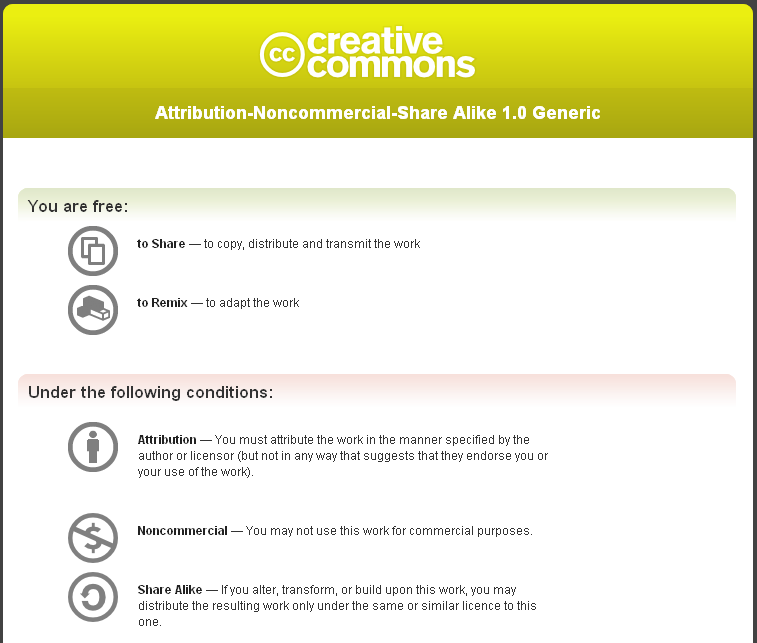
\includegraphics[width=0.74\textwidth]
		{pics/creative_common.png}
	\caption{\license}
	\label{fig:lisensi}
\end{figure}

\pic~\ref{fig:lisensi} diambil dari 
\url{http://creativecommons.org/licenses/by-nc-sa/1.0/deed.en_CA}. 
Jika ingin mengentahui lebih lengkap mengenai \license, silahkan buka 
\url{http://creativecommons.org/licenses/by-nc-sa/1.0/legalcode}. 
Seluruh dokumen yang dibuat dengan menggunakan template ini sepenuhnya 
menjadi hak milik pembuat dokumen dan bebas didistribusikan sesuai dengan 
keperluan masing-masing. 
Lisensi hanya berlaku jika ada orang yang membuat template baru dengan 
menggunakan template ini sebagai dasarnya. 

Dokumen ini dibuat dengan \latex~juga. Untuk meyakinkan Anda, coba lihat 
properti dari dokumen ini dan Anda akan menemukan bagian seperti 
\pic~\ref{fig:pdflatex}. 
Dokumen ini dimaksudkan untuk memberikan gambaran kepada Anda seperti apa 
mudahnya menggunakan \latex~dan juga memperlihatkan betapa bagus dokumen 
yang dihasilkan. 
Seluruh url yang Anda temukan dapat Anda klik. 
Seluruh referensi yang ada juga dapat diklik. 
Untuk mengerti template yang disediakan, Anda tetap harus membuka kode 
\latex~dan bermain-main dengannya. 
Penjelasan dalam PDF ini masih bersifat gambaran dan tidak begitu 
mendetail, dapat dianggap sebagai pengantar singkat. 
Jika Anda merasa kesulitan dengan template ini, mungkin ada baiknya 
Anda belajar sedikit dasar-dasar \latex. 

\begin{figure}
	\centering
	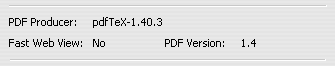
\includegraphics[width=0.54\textwidth]
		{pics/mark.png}
	\caption{Dokumen Dibuat dengan PDFLatex}
	\label{fig:pdflatex}
\end{figure}

Semoga template ini dapat membantu orang-orang yang ingin mencoba menggunakan 
\latex. Semoga template ini juga tidak berhenti disini dengan ada kontribusi 
dari para penggunanya. 
Kami juga ingin berterima kasih kepada Andreas Febrian, Lia Sadita, Fahrurrozi 
Rahman, Andre Tampubolon, dan Erik Dominikus atas kontribusinya dalam template 
ini. 

\vspace*{0.1cm}
\begin{flushright}
Bandung, XX Januari 2016\\[0.1cm]
\vspace*{1cm}
\penulis

\end{flushright}
%
%
\addChapter{LEMBAR PERSETUJUAN PUBLIKASI ILMIAH}
% 
% @author  Andre Tampubolon, Andreas Febrian
% @version 1.01
% 

\chapter*{\uppercase{Halaman Pernyataan Persetujuan Publikasi Tugas Akhir untuk Kepentingan Akademis}}

\vspace*{0.2cm}
\noindent 
Sebagai sivitas akademik Universitas Indonesia, saya yang bertanda 
tangan di bawah ini:
\vspace*{0.4cm}


\begin{tabular}{p{4.2cm} l p{6cm}}
	\bo{Nama} & : & \penulis \\ 	
	\bo{NPM} & : & \npm \\
	\bo{Program Studi} & : & \program\\	
	\bo{Fakultas} & : & \fakultas\\
	\bo{Jenis Karya} & : & \type \\
\end{tabular}

\vspace*{0.6cm}
\noindent demi pengembangan ilmu pengetahuan, menyetujui untuk memberikan 
kepada Universitas Indonesia \bo{Hak Bebas Royalti Noneksklusif 
(Non-exclusive Royalty Free Right)} atas karya ilmiah saya yang berjudul:
\begin{center}
	\judul
\end{center}
beserta perangkat yang ada (jika diperlukan). Dengan Hak Bebas Royalti 
Noneksklusif ini Universitas Indonesia berhak menyimpan, 
mengalihmedia/formatkan, mengelola dalam bentuk pangkalan data 
(database), merawat, dan memublikasikan tugas akhir saya selama 
tetap mencantumkan nama saya sebagai penulis/pencipta dan sebagai 
pemilik Hak Cipta. \\

\noindent Demikian pernyatan ini saya buat dengan sebenarnya.

\begin{center}
	\vspace*{0.8cm}
	\begin{tabular}{lll}
		Dibuat di&: & Bandung \\
		Pada tanggal&: & \tanggalPengesahan \\
	\end{tabular}\\

	\vspace*{0.2cm}
	Yang menyatakan \\
	\vspace*{1.1cm}
	(\penulis)
\end{center}

\newpage


%
% 
\addChapter{ABSTRAK}
%
% Halaman Abstrak
%
% @author  Andreas Febrian
% @version 1.00
%

\chapter*{Abstrak}

\vspace*{0.2cm}

\begin{center}
	{\large \textbf{PERANCANGAN SISTEM REKOMENDASI LOKASI PENCACAHAN SECARA \textit{REAL-TIME} BERBASIS KONTEKS}} \\
	\vspace*{0.2cm}
	Oleh \\
	{\large \textbf{Aris Prawisudatama}} \\
	{\large \textbf{NIM: 23215131}} \\
	{\large \textbf{(Program Studi Magister Teknik Elektro)}}
\end{center}


\vspace*{0.5cm}

\noindent Pengumpulan data lapangan merupakan salah satu tugas dan kewenangan yang dimiliki oleh institusi statistik sebuah negara, tidak terkecuali Badan Pusat Statistik (BPS). Pada praktiknya, BPS menggunakan Blok Sensus (BS) yang merupakan wilayah kerja dari seorang petugas pencacahan. Pengalokasian wilayah kerja seringkali dilakukan secara subyektif, sehingga menimbulkan ketimpangan waktu penyelesaian antar petugas pencacahan, yang pada akhirnya menyebabkan keterlambatan kegiatan pengumpulan data secara keseluruhan. Walaupun permasalahan alokasi petugas pengumpulan data memiliki kemiripan dengan permasalahan \textit{Multi Depot Vehicle Routing Problem} (VRP), algoritma penyelesaian MDVRP tidak serta merta dapat digunakan, karena informasi terkait lama pencacahan pada suatu wilayah kerja tidak tersedia. \\

\noindent Pada penelitian ini diusulkan sebuah sistem yang dapat digunakan untuk membuat rekomendasi yang lebih merata. Sistem usulan bekerja secara bertahap, dengan menggabungkan algoritma penyelesaian MDVRP dengan mekanisme \textit{Publish/Subscribe}. Agar rekomendasi yang dibuat oleh sistem akurat, digunakan konteks dari setiap petugas pada saat pencarian solusi. \\

\noindent Pengujian dilakukan dengan membandingkan sistem usulan dengan program pembanding, yaitu algoritma MDVRP tanpa menggunakan mekanisme Publish/Subscribe. Berdasarkan hasil pengujian, sistem usulan dapat memberikan rekomendasi dengan lebih efisien pada sebagaian besar kasus.  \\

\vspace*{0.2cm}

\noindent Kata Kunci: rekomendasi; \textit{location routing}; VRP; MDVRP; \textit{publish/subscribe} \\

\newpage
%
%
\addChapter{ABSTRACT}
%
% Halaman Abstract
%
% @author  Andreas Febrian
% @version 1.00
%

\chapter*{ABSTRACT}

\vspace*{0.2cm}

\noindent \begin{tabular}{l l p{11.0cm}}
	Name&: & \penulis \\
	Program&: & \program \\
	Title&: & \judulInggris \\
\end{tabular} \\ 

\vspace*{0.5cm}

\noindent \todo{Write your abstract here.}\\

\vspace*{0.2cm}

\noindent Keywords: \\ 
\noindent \todo{Write up keywords about your report here.}

\newpage

%
% Daftar isi, gambar, dan tabel
%
\tableofcontents
\clearpage
\listoffigures
\clearpage
\listoftables
\clearpage
\listofalgorithms
\clearpage
\listoflistings
\clearpage

%
% Gunakan penomeran Arab (1, 2, 3, ...) setelah bagian ini.
%
\pagenumbering{arabic}

%
%
%
%-----------------------------------------------------------------------------%
\chapter{\babSatu}
%-----------------------------------------------------------------------------%

\section{Latar Belakang}

Badan Pusat Statistik (BPS) merupakan suatu lembaga pemerintah non-departemen yang bertanggung jawab dalam penyediaan statistik dasar \citep{bps_badan_2016}. Dalam peranannya sebagai penyedia data, BPS melakukan pengumpulan data dengan 2 (dua) metode, yaitu primer dan sekunder. Pengumpulan data primer adalah pengumpulan data dengan menggunakan metode wawancara langsung dengan responden, baik responden individu, rumah tangga, maupun perusahaan. Sementara pengumpulan data sekunder adalah pengumpulan data dengan memanfaatkan data yang telah dikumpulkan oleh pihak lain.


Pada pengumpulan data primer oleh BPS, selanjutnya disebut dengan pencacahan, suatu wilayah administratif dibagi dalam beberapa Blok Sensus (BS). Blok sensus merupakan wilayah kerja dari seorang pencacah \citep{bps_sistem_2016}. Setiap petugas pengumpulan data, disebut dengan pencacah, akan dialokasikan dalam beberapa blok sensus yang akan menjadi tanggung jawabnya. Pencacah kemudian akan mendatangi blok sensus tersebut dan mengunjugi setiap rumah tangga yang menjadi sampel pencacahan.


\begin{figure}[h]
    \centering
    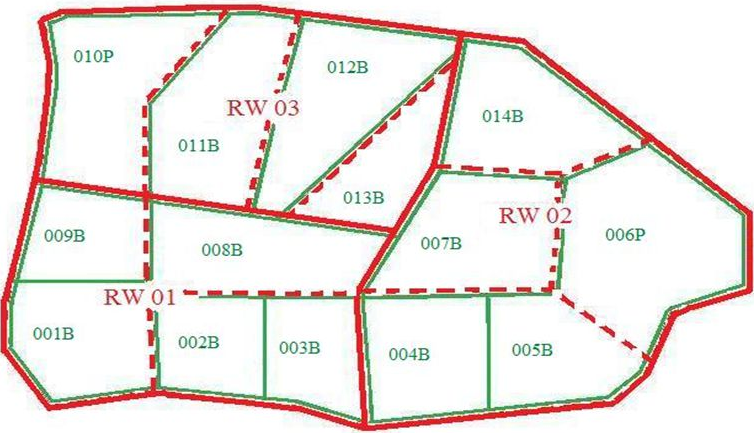
\includegraphics[width=10cm]{../../Resources/Images/peta_kelurahan_per_bs}
    \caption{Pembagian Blok Sensus dalam Desa/Kelurahan}
    \label{fig:capi-ilustration}
\end{figure}


Pengalokasian pencacah terhadap blok sensus terkadang menjadi sesuatu yang sulit, karena terkait dengan waktu dan biaya. \textit{Subject matter} yang menangani kegiatan harus mempertimbangkan beberapa hal, salah satunya adalah jarak antar blok sensus yang menjadi wilayah kerja seorang pencacah. Kesalahan dalam pengalokasian blok sensus menyebabkan waktu pencacahan menjadi lama, yang dapat mempengaruhi kegiatan pencacahan secara keseluruhan.


Selain jarak antar blok sensus, faktor yang juga perlu diperhatikan adalah lamanya pencacahan dalam sebuah blok sensus. Lama pencacahan dalam blok sensus secara umum dipengaruhi oleh 2 (dua) faktor, jarak antar rumah tangga dalam suatu blok sensus dan lama wawancara dalam rumah tangga. \citep{sudman_time_1965}, dalam penelitiannya menyatakan bahwa mengunjungi sebuah segmen dapat menghabiskan 21 persen dari keseluruhan waktu, 15 persen untuk mengunjungi rumah tangga dalam sebuah segmen, 37 persen untuk wawancara, dan sisanya untuk kegiatan lain, seperti \textit{editing}, \textit{study}, dan \textit{clerical}.


Faktor-faktor yang terkait dengan alokasi blok sensus dan petugas tersebut diatas, seperti: jarak antar blok sensus, jarak antar rumah tangga, dan lama wawancara tidaklah selalu tersedia. Andaikan tersedia, datanya-pun bersifat relatif, seperti lama wawancara yang sangat tergantung pada kemampuan pencacah dalam bertanya dan menggali jawaban, tingkat pendidikan responden, dan banyaknya anggota rumah tangga yang harus didata. Oleh karena itu diperlukan suatu cara atau metode yang memungkinkan pengalokasian petugas terhadap blok sensus secara dinamis sesuai dengan context.


Dalam sistem komputer tidak terdapat definisi \textit{context} yang tunggal. Meskipun demikian, sebagian besar definisi sepakat bahwasannya \textit{context} adalah sesuatu yang harus dilakukan terkait interaksi pengguna dan sistem komputer \citep{chen_survey_2000}. \citep{schilit_context-aware_1994}, misalnya, membagi \textit{context} menjadi 4 (empat): \textit{computing context}, \textit{user context}, \textit{physical context}, dan \textit{time context}. \textit{Computing context} meliputi: \textit{network connectivity}, \textit{communication cost}, \textit{communication bandwidth}, dan \textit{nearby resource}; \textit{user context} meliputi: \textit{user profile}, \textit{location}, dan \textit{social situation}; \textit{physical context} meliputi: \textit{lighting}, \textit{noise}, \textit{traffic condition}, dan \textit{temperature}; serta \textit{time context} meliputi: \textit{time of a day}, \textit{week}, \textit{month} and \textit{season of the year}. Senada dengan \citep{schilit_context-aware_1994}, \citep{schmidt_there_1999} mendefinisikan \textit{context} sebagai pengetahuan tentang \textit{state} dari \textit{user} dan \textit{IT device}, termasuk lingkungan, situasi, dan lokasi. Sementara \citep{abowd_towards_1999} mendefinisikan \textit{context} sebagai segala informasi yang dapat digunakan untuk mengkarakterisasi kondisi dari suatu entitas. Entitas yang dimaksud dapat berupa manusia, tempat atau obyek yang relevan dengan aplikasi dan pengguna, termasuk aplikasi dan pengguna itu sendiri. 


\begin{figure}[h]
    \centering
    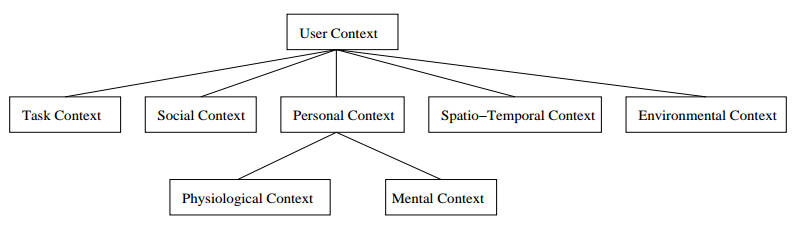
\includegraphics[width=\textwidth]{../../Resources/Images/context}
    \caption{Context Hierarchy \citep{kofod-petersen_case-based_2003}}
    \label{fig:capi-ilustration}
\end{figure}


\textit{Context-aware application} telah banyak digunakan di berbagai bidang. \citep{tsai_context-aware_2016} misalnya, menggunakan \textit{context} untuk menciptakan \textit{smart home environment}. \citep{magara_mplist:_2016} menggabungkan beberapa \textit{context} seperti: lokasi dan aktivitas pengguna, preferensi, label, dan \textit{tags} untuk membuat rekomendasi musik yang akan diputar. Sementara \citep{said_introduction_2013} menciptakan rekomendasi film berdasarkan \textit{time}, \textit{mood}, dan \textit{social recommendation}.


Pada aplikasi yang bersifat \textit{mobile}, \textit{context} biasanya diperoleh dengan menggunakan sensor yang tersemat dalam \textit{mobile device} tersebut. Sekarang ini, telah banyak ditemui \textit{mobile device}, terutama \textit{programmable smartphone}, yang telah dilengkapi dengan berbagai sensor \citep{cao_mobile_2015}. \citep{do_groupus:_2011}, misalnya mem-\textit{propose} GroupUs, framework yang mengelompokkan pengguna berdasarkan aktifitas sehari-hari yang dikumpulkan dengan menggunakan \textit{proximity sensor}. \citep{dai_mobile_2010} menciptakan \textit{drunk driving detection} dengan memanfaatkan sensor \textit{accelerometer} yang tersemat dalam \textit{smartphone}. Sementara \citep{zou_context-aware_2016}, memanfaatkan sensor \textit{Global Posisioning System} (GPS) dan \textit{Micro-Electro-Mechanical System} (MEMS) untuk membuat rekomendasi transportasi. Begitu pula sensor-sensor yang lain juga telah dimanfaatkan dalam berbagai penelitian \citep{dai_perfalld:_2010, lu_soundsense:_2009, bao_movi:_2010, rubel_toward_2005, atzmueller_towards_2013}.


Di sisi yang lain, \textit{location recommendation} merupakan sebuah bahasan yang juga banyak diteliti. Metode yang banyak digunakan untuk menentukan rekomendasi lokasi adalah \textit{Location-based Social Network} (LBSN). Cara kerja LBSN pada dasarnya adalah dengan memanfaatkan lokasi dan \textit{point of interest} yang dibagikan oleh pengguna \citep{yuan_location_2016}. Beberapa peneliti juga mencoba meningkatkan akurasi prediksi dengan menggabungkannya dengan berbagai metode. Misalnya \citep{koren_collaborative_2010}, menggunakan \textit{temporal factorization model} yang memberikan hasil lebih baik dibanding dengan \textit{non-temporal factorization model}. Sementara  \citep{pragarauskas_temporal_2010} mengadopsi \textit{bayesian probabilistic tensor factorization} untuk mewujudkan \textit{temporal collaborative filtering}. Akan tetapi, metode LBSN tidak sesuai digunakan untuk membuat rekomendasi lokasi pencacahan. Hal ini dikarenakan metode LBSN menggunakan \textit{logs} yang telah dikumpulkan sebelumnya, baik \textit{location logs} maupun \textit{user preference logs}, untuk menentukan rekomendasi, sementara lokasi pencacahan bukan merupakan \textit{point of interest} yang dikunjungi oleh banyak orang.


Metode lain yang juga banyak digunakan adalah \textit{Travelling Salesman Problem} (TSP). TSP adalah sebuah algoritma klasik \citep{biggs_graph_1976} yang telah banyak diadopsi dan dimodifikasi. Masalah yang umumnya mejadi dasar modifikasi adalah penggunaan \textit{multiple salesman}, yang disebut dengan \textit{Multiple Travelling Salesman Problem} (MTSP) \citep{bektas_multiple_2006}. Variasi dari MTSP juga telah banyak diteliti, yang umumnya mencakup: \textit{single or multiple depots} (\textit{start and stop point}), jumlah \textit{salesman}, \textit{fixed charges} (jika jumlah \textit{salesman} tidak tetap), lama kunjungan (\textit{time window}), dan \textit{special restrictions} \citep{bektas_multiple_2006}. Berbagai aplikasi untuk menyelesaikan permasalahan nyata (\textit{real-life problem}) juga telah dikembangkan dengan menggunakan MTSP. Misalnya, \textit{print press scheduling} oleh \citep{gorenstein_printing_1970}, \textit{crew scheduling} oleh \citep{svestka_computational_1973}, \textit{school bus routing problem} oleh \citep{angel_computer-assisted_1972}, \textit{interview scheduling} oleh \citep{gilbert_new_1992}, \textit{mission planning} oleh \citep{brumitt_dynamic_1996}, \textit{hot rolling scheduling} oleh \citep{tang_multiple_2000}, dan \textit{global navigation satellite system surveying networks} oleh \citep{saleh_design_2004}.


\begin{figure}[h]
    \centering
    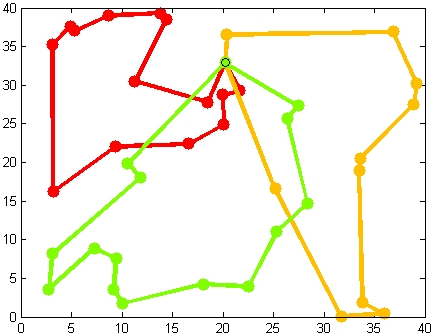
\includegraphics[width=10cm]{../../Resources/Images/mtsp}
    \caption{Ilustrasi \textit{Multiple Travelling Salesman Problem}}
    \label{fig:mtsp-ilustration}
\end{figure}


Asumsi yang digunakan dalam pendekatan MTSP adalah semua informasi telah tersedia pada saat perancangan, sehingga rekomendasi \textit{path} telah diperoleh sebelum kunjungan pertama. Sementara dalam pencacahan, informasi tidak selalu tersedia. Misalnya \textit{service-time}, yang tersusun atas jarak antar rumah tangga dan lama wawancara, merupakan variabel yang bersifat dinamis. Jarak antar rumah tangga sangat tergantung dari sampel yang terpilih, sementara lama wawancara sangat tergantung dari beberapa faktor, seperti: kemampuan pencacah dalam bertanya dan menggali jawaban, kemampuan responden dalam mencerna pertanyaan pencacah, dan banyaknya anggota rumah tangga yang harus didata. Untuk itu, diperlukan suatu metode agar implementasi MTSP untuk rekomendasi lokasi pencacahan dapat mengakomodir \textit{service-time} secara dinamis.


Solusi yang ditawarkan adalah dengan mengabaikan \textit{service-time}, kemudian meng-\textit{generate} rekomendasi baru setiap kali pencacah telah menyelesaikan pencacahan pada suatu blok sensus. Untuk itu, pendekatan MTSP ini akan digabung dengan metode \textit{Publish/Subsribe}. Publish/Subsribe atau pub/sub adalah paradigma dimana \textit{user} mengekspresikan ketertarikan-nya (\textit{subscriptions}), dan agen menerbitkan beberapa penawaran-nya (\textit{event}) \citep{fabret_filtering_2001}. Metode pub/sub yang akan digunakan adalah pub/sub \textit{location-based tracking service}, sebagaimana diusulkan oleh \citep{chen_efficient_2003}.


\section{Rumusan Masalah}

Berdasarkan latar belakang permasalahan yang telah diuraikan sebelumnya, dan didasari motivasi untuk menciptakan rekomendasi alokasi pencacah dan blok sensus secara dinamis, maka dapat dirumuskan masalah dalam penelitian ini adalah bagaimana merancang sebuah sistem rekomendasi lokasi pencacahan dengan memanfaatkan \textit{context} dari pencacah.


Adapun detail dari permasalahan yang akan dikaji adalah sebagai berikut:

\begin{itemize}
\item Bagaimana menentukan \textit{context} apa saja yang dapat digunakan dalam kasus ini.
\item Bagaimana membuat rekomendasi lokasi pencacahan pada kondisi \textit{time windows} sangat berpengaruh, tetapi data tidak tersedia.
\item Bagaimana membuat \textit{conflict resolution}, agar dua atau lebih \textit{smartphone} tidak merekomendasikan lokasi yang sama.
\end{itemize}


\section{Tujuan Penelitian}

Berdasarkan rumusan masalah diatas, maka dapat ditentukan tujuan utama dari penelitian ini adalah untuk menciptakan sebuah sistem rekomendasi lokasi pencacahan secara dinamis. 

Adapun tujuan khusus dari penelitian ini adalah:

\begin{itemize}
\item Mengidentifikasi \textit{context} yang terkait dengan penentuan lokasi pencacahan.
\item Menyusun algoritma rekomendasi.
\item Menyusun algoritma \textit{location conflict}.
\item Mengimplementasikan algoritma usulan dalam \textit{mobile application}.
\item Melakukan ujicoba algoritma dan aplikasi usulan.
\end{itemize}


\section{Batasan Masalah}

Masalah dalam penelitian ini memiliki batasan sebagai berikut:

\begin{itemize}
\item Lokasi pencacahan yang menjadi rujukan adalah Blok Sensus (BS) yang dikeluarkan oleh Badan Pusat Statistik (BPS).
\item \textit{Device} yang digunakan adalah \textit{smartphone} berbasis Android yang umum dijual dipasaran.
\item Tidak mempertimbangkan lingkungan yang tidak terkoneksi dengan jaringan komunikasi.
\end{itemize}


\section{Implikasi}

Manfaat yang dapat diperoleh dari penelitian ini antara lain:


\section{Sistematika Penulisan}

Sistematika penulisan tesis ini terdiri atas enam bab dengan perincian sebagai berikut:

%-----------------------------------------------------------------------------%
\chapter{\babDua}
%-----------------------------------------------------------------------------%


%-----------------------------------------------------------------------------%
\section{\textit{Literature Map}}
\label{sec:literature-map}
%-----------------------------------------------------------------------------%
\textit{Literature Map} merupakan sebuah visualisasi yang memuat \textit{summary} penelitian terkait yang telah dilakukan sebelumnya. \textit{Literature Map} biasanya direpresentasikan dalam sebuah gambar, misalnya menggunakan struktur hierarki \textit{top-down} dalam mempresentasikan literatur \citep{creswell_research_2013}. Ide utama dari penggambaran \textit{literature map} adalah untuk membuat visualisasi dari penelitian terdahulu tentang sebuah topik. 

\begin{figure}[!]
	\centering
	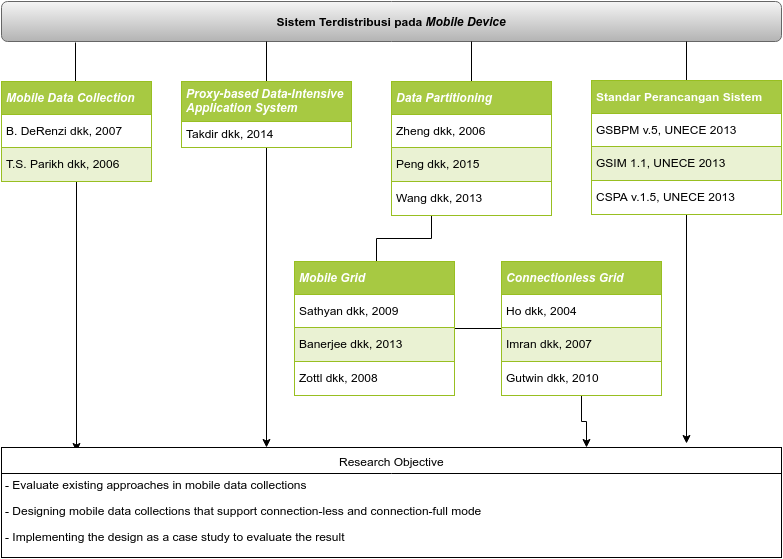
\includegraphics[width=\textwidth]{Resources/Images/literature-map}
	\captionsetup{format=hang}
	\caption{\textit{Literature Map} Penelitian}
	\label{fig:literature-map}
\end{figure}


Berdasarkan review dari literatur yang terkait dengan penelitian ini (\autoref{fig:literature-map}), arsitektur dari rekomendasi lokasi pada pengumpulan data lapangan dapat dibagi menjadi 3 (tiga) kelompok: \textit{context-aware computing}, \textit{location routing}, dan mekanisme komunikasi.


\textit{Context-aware computing} akan membahas beberapa literatur yang berkaitan dengan definisi dari konteks itu sendiri dan pemanfaatannya dalam komputasi. \textit{Location routing} akan membahas literatur terkait beberapa algoritma yang biasa digunakan dalam penyelesaian masalah \textit{location routing}. Sementara mekanisme komunikasi akan mendiskusikan tentang beberapa metode yang dapat digunakan oleh \textit{client} dan \textit{server} dalam berkormunikasi.


%-----------------------------------------------------------------------------%
\section{Badan Pusat Statistik}
\label{sec:badan-pusat-statistik}
%-----------------------------------------------------------------------------%
Badan Pusat Statistik (BPS) adalah Lembaga Pemerintah Non-Departemen yang bertanggung jawab dan memiliki peranan dalam penyediaan data. Berdasarkan Rencana Strategis BPS 2015-2019, BPS memiliki misi yang harus dijalankan yaitu:
\begin{enumerate}
\item Menyediakan data statistik berkualitas melalui kegiatan statistik yang terintegrasi dan berstandar nasional maupun internasional. \\
Dalam rangka menyediakan data berkualitas, data yang dihasilkan BPS harus memenuhi dimensi kualitas yakni relevan, akurat, disajikan tepat waktu, koheren, dapat diakses, dan dapat diinterpretasikan.
\item Memperkuat Sistem Statistik Nasional yang berkesinambungan melalui pembinaan dan koordinasi di bidang statistik.
\item Membangun insan statistik yang profesional, berintegritas dan amanah untuk kemajuan perstatistikan.
Dalam menyelenggarakan kegiatan statistik, insan statistik harus memiliki kapasitas dan kapabilitas yang diperlukan untuk menghasilkan data statistik yang berkualitas.
\end{enumerate}


Di dalam menjalankan peranan sebagai penyedia data, BPS menyelenggarakan statistik dasar dengan cara sensus, survei, dan kompilasi administrasi untuk mendapatkan data. Data yang berkualitas hanya dapat diperoleh melalui proses yang berkualitas pula. Terdapat berbagai variabel yang menjadi parameter proses yang berkualitas, salah satunya adalah ketepatan waktu dalam proses pengumpulan data.

Pengumpulan data merupakan suatu proses yang sangat fleksibel. Ketepatan waktu pengumpulan data sangat rentan terhadap pengaruh berbagai faktor, seperti kualitas petugas pengumpulan data, kualitas responden, jumlah anggota rumah tangga yang didata, jarak antar lokasi pencacahan, jarak antar rumah tangga dalam satu segmen, dan kondisi alam. Alokasi petugas pengumpulan data secara baku yang hanya memperhatikan jumlah lokasi pencacahan dan petugas, tidak dapat mengakomodir faktor-faktor tersebut. Akibatnya, waktu penyelesaian pengumpulan data bisa bervariasi antara satu petugas dengan petugas lainnya. Oleh karena itu, diperlukan suatu metode baru dalam pengalokasian petugas yang dapat mengantisipasi terjadinya kesenjangan beban tugas baik dari segi waktu maupun kuantitas.  

%-----------------------------------------------------------------------------%
\section{\textit{Context-aware Computing}}
\label{sec:context-aware-computing}
%-----------------------------------------------------------------------------%


%-----------------------------------------------------------------------------%
\subsection{Definisi \textit{Context}}
\label{ssec:context-definition}
%-----------------------------------------------------------------------------%
Semenjak \textit{Context-aware computing} pertama kali diperkenalkan oleh \citep{schilit_context-aware_1994}, berbagai definisi mengenai \textit{context} dan \textit{context-awareness} telah berkembang luas. Sebagaian besar definisi yang ada saat ini, menurut \citep{zimmermann_operational_2007}, dapat dikelompokkan menjadi dua: definisi menurut sinonim dan definisi menurut contoh. \textit{Context} mengalami berbagai penggolongan menggunakan sinonim seperti \textit{application environment} \citep{hull_towards_1997} atau situasi \citep{brown_stick-e_1995}. Sementara beberapa authors, seperti \citep{brown_context-aware_1997}, \citep{gross_awareness_2001}, dan \citep{ryan_enhanced_1999}, mendefinisikan \textit{context by example} dan \textit{context element} seperti lokasi, identitas, waktu, suhu, kebisingan sama dengan kepercayaan, keinginan, komitmen, dan hubungan dengan manusia \citep{chen_intelligent_2003}.


Secara umum, dapat dikatakan bahwasanya \textit{context} adalah informasi yang dapat digunakan dalam menjelaskan situasi dari sebuah entitas. Entitas dapat dapat berupa manusia, lokasi, atau obyek yang relevan dengan interaksi antara seorang pengguna dan aplikasi, termasuk pengguna dan aplikasi itu sendiri \citep{dey_understanding_2001}. \citep{schilit_context-aware_1994} menyebutkan bahwa yang termasuk ke dalam \textit{context} adalah: lokasi dari penggunaan, kumpulan orang-orang sekitar, \textit{hosts}, dan \textit{accessible devices}, serta perubahan hal-hal tersebut dari waktu ke waktu. \citep{dey_understanding_2001} mengembangkan definisi dari \citep{schilit_context-aware_1994} dengan menyatakan "\textit{Context} adalah lokasi, identitas dan status dari individu, kelompok, dan obyek komputasi".


%-----------------------------------------------------------------------------%
\subsection{Kategori \textit{Context}}
\label{ssec:context-category}
%-----------------------------------------------------------------------------%
Dari berbagai informasi yang menjelaskan entitas dari \textit{context}, semuanya mengarah ke 5 (lima) kategori, yaitu: \textit{individuality}, aktivitas, lokasi, waktu, dan relasi, seperti pada Gambar \ref{fig:context-categories} \citep{zimmermann_operational_2007}. Kategori \textit{individuality} memuat properti dan atribut yang menjelaskan entitas itu sendiri. Kategori aktivitas mencakup seluruh kegiatan yang dilakukan entitas tersebut. Kategori lokasi dan waktu menyediakan koordinat \textit{spatio-temporal} dari entitas. Sementara kategori relasi merepresentasikan informasi tentang hubungan antara sebuah entitas dengan entitas yang lain.


\begin{figure}[!]
	\centering
	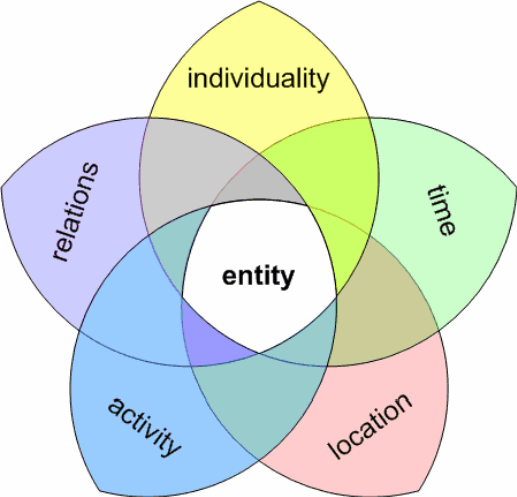
\includegraphics[width=6cm]{Resources/Images/context-categories}
	\captionsetup{format=hang}
	\caption{Kategori dari \textit{Context}}
	\label{fig:context-categories}
\end{figure}


%-----------------------------------------------------------------------------%
\subsubsection{\textit{Individuality Context}}
\label{sssec:individuality-context}
%-----------------------------------------------------------------------------%
Kategori ini memberi akses kepada informasi yang bersifat kontekstual tentang entitas terkait. Informasi ini dapat berupa apa saja terkait entitas tersebut, tetapi umumnya adalah \textit{state} dari entitas. Entitas dapat berupa entitas individu atau sekelompok entitas yang saling berbagi \textit{context} yang terkait. Entitas dapat berupa entitas yang \textit{real} (eksis secara nyata), maupun virtual (hanya terdapat di lingkup informasi). Selain itu, terdapat juga entitas yang bersifat \textit{mobile}, \textit{movable}, maupun \textit{fixed}. kategori \textit{inviduality context} dikelompokkan menjadi empat, yaitu: \textit{natural}, \textit{human}, \textit{artificial}, dan \textit{group entities}.


%-----------------------------------------------------------------------------%
\subsubsection{\textit{Time Context}}
\label{sssec:time-context}
%-----------------------------------------------------------------------------%
Waktu merupakan aspek yang vital dalam klasifikasi \textit{context}, karena sebagian besar pernyataan sangat terkait dengan dimensi \textit{temporal}. Kategori ini menkalkulasi informasi seperti \textit{time zone} dari \textit{client}, dan \textit{current time} atau \textit{virtual time}. Contoh representasi dari waktu adalah \textit{time zone}, misalnya format \textit{ Central European Time (CET)}, yang menyediakan fasilitas kalkulasi secara matematis dan komparasi waktu. Model dimensi waktu yang sering diimplementasikan dalam \textit{context-aware computing} misalnya jam kerja atau hari libur.


\textit{Context} yang disimpan secara persisten dapat membentuk sebuah \textit{data pool} yang berisi histori dari informasi terkait \textit{context} tersebut. Histori tersebut membentuk basis data untuk \textit{context information} dari event yang telah lampau. Basis data yang dipersistenkan dapa digunakan sebagai bahan analisis dari kebiasaan dari pengguna dan prediksi.


%-----------------------------------------------------------------------------%
\subsubsection{\textit{Location Context}}
\label{sssec:location-context}
%-----------------------------------------------------------------------------%
Dengan semakin berkembangnya \textit{portable/mobile devices}, lokasi menjadi parameter yang penting dalam \textit{context-aware system}. Obyek-obyek fisik dan perangkat tersusun secara spasial, dipengaruhi oleh pergerakan pengguna. Kategori ini berisi model lokasi yang terklasifikasi secara fisik maupun virtual, misalnya \textit{IP address} sebagai posisi komputer dalam sebuah jaringan, koordinat, maupun informasi spasial terkait seperti kecepatan dan orientasi. Lokasi dapat berupa lokasi absolut atau lokasi relatf, yaitu lokasi yang diperhitungkan dari objek yang lain. Model dapat juga terdiri dari lokasi kuantitatif (geometrik) dan kualitatif (simbol).


Lokasi yang bersifat kuantitatif merujuk kepada koordinat dengan dua dimensi, tiga dimensi, atau lebih. Sebagai contoh, koordinat dua dimensi secara geografis melambangkan setiap lokasi di bumi secara lintang dan bujur. Informasi terkait koordinat geografis biasanya diperoleh melalui \textit{Global Posisitioning System} dengan menggunakan satelit. Selain itu, lokasi juga dapat diklasifikasikan menjadi dalam dan luar ruangan, sinyal radio atau cahaya, dll. Sementara itu, lokasi yang bersifat kualitatif dan berupa bangunan, ruangan, jalan, negara, dan sebagainya. 


%-----------------------------------------------------------------------------%
\subsubsection{\textit{Activity Context}}
\label{sssec:activity-context}
%-----------------------------------------------------------------------------%
\textit{Context} aktivitas meliputi aktivitas yang sedang dikerjakan oleh sebuah entitas. Kategori ini dapat diterjemahkan menjadi: tujuan, kegiatan, dan aksi. Sebuah \textit{task} merupakan aktivitas yang berorientasi pada capaian. Capaian atau \textit{goals} dapat bersifat \textit{low-level}, dimana \textit{goal} dapat sering berganti, atau \textit{high-level}, dimana \textit{goal} bersifat konsisten.


%-----------------------------------------------------------------------------%
\subsubsection{\textit{Relations Context}}
\label{sssec:relations-context}
%-----------------------------------------------------------------------------%
Kategori ini mencakup relasi dari sebuah entitas yang berhubungan dengan entitas yang lain. Entitas yang lain tersebut dapat berupa manusia, benda, layanan, atau informasi (misalnya teks, gambar, film, suara). Karakteristik dari \textit{environment} biasanya dibangun secara spasial dan temporal. Individu dalam kelompok saling mempengaruhi kelompok dalam satu relasi, misalnya seluruh manusia dengan umur yang sama.


%-----------------------------------------------------------------------------%
\subsection{\textit{Context-aware Computing}}
\label{ssec:context-aware-computing}
%-----------------------------------------------------------------------------%
\citep{dey_understanding_2001} menjelaskan, sebuah sistem dikatakan \textit{context-aware} jika dia menggunakan \textit{context} untuk menyediakan informasi atau layanan yang relevan kepada pengguna, dimana relevansinya tergantung dari apa yang pengguna kerjakan.


Terdapat berbagai contoh sistem yang bersifat \textit{context-aware}. \citep{tsai_context-aware_2016} misalnya, menggunakan \textit{context} untuk menciptakan \textit{smart home environment}. \citep{magara_mplist:_2016} menggabungkan beberapa \textit{context} seperti: lokasi dan aktivitas pengguna, preferensi, label, dan \textit{tags} untuk membuat rekomendasi musik yang akan diputar. Sementara \citep{said_introduction_2013} menciptakan rekomendasi film berdasarkan \textit{time}, \textit{mood}, dan \textit{social recommendation}.


Pada aplikasi yang bersifat \textit{mobile}, \textit{context} biasanya diperoleh dengan menggunakan sensor yang tersemat dalam \textit{mobile device} tersebut. Sekarang ini, telah banyak ditemui \textit{mobile device}, terutama \textit{programmable smartphone}, yang telah dilengkapi dengan berbagai sensor \citep{cao_mobile_2015}. \citep{do_groupus:_2011}, misalnya mem-\textit{propose} GroupUs, framework yang mengelompokkan pengguna berdasarkan aktivitas sehari-hari yang dikumpulkan dengan menggunakan \textit{proximity sensor}. \citep{dai_mobile_2010} menciptakan \textit{drunk driving detection} dengan memanfaatkan sensor \textit{accelerometer} yang tersemat dalam \textit{smartphone}. Sementara \citep{zou_context-aware_2016}, memanfaatkan sensor \textit{Global Posisioning System} (GPS) dan \textit{Micro-Electro-Mechanical System} (MEMS) untuk membuat rekomendasi transportasi. Begitu pula sensor-sensor yang lain juga telah dimanfaatkan dalam berbagai penelitian \citep{dai_perfalld:_2010, lu_soundsense:_2009, bao_movi:_2010, rubel_toward_2005, atzmueller_towards_2013}.


Pada kasus yang dijadikan dasar dari penelitian ini, yaitu terkait pengumpulan data lapangan, \textit{context} yang akan digunakan adalah \textit{spatio-temporal context}, yang meliputi lokasi dan waktu dari setiap pencacah.


%-----------------------------------------------------------------------------%
\section{\textit{Location Routing}}
\label{sec:location-routing}
%-----------------------------------------------------------------------------%
\textit{Location routing problem} (LRP), menurut \citep{nagy_location-routing:_2007}, secara umum dapat dikatakan sebagai sebuah pendekatan dalam pemodelan dan penyelesaian permasalahan terkait lokasi. Definisi ini mengikuti konsep dari \citep{bruns_zweistufige_1998}, yaitu perencanaan lokasi yang mempertimbangkan perencanaan \textit{tour}. Definisi ini juga senada dengan \citep{balakrishnan_integrated_1987}, yang menyatakan bahwa \textit{location routing problem} merupakan keputusan strategis yang berfokus pada lokasi fasilitas.


Lokasi dari fasilitas dan \textit{vehicle routing} merupakan area yang saling terkait. \citep{maranzana_location_1964} menyatakan bahwa "\textit{the location of factories, warehouses and supply points in general...is often influenced by transport costs."}. Tetapi beberapa peneliti, sebagaimana \citep{nagy_location-routing:_2007}, menolak korelasi tersebut dengan beberapa alasan:

\begin{enumerate}
\item Terdapat beberapa kondisi dimana \textit{location problem} tidak memiliki aspek \textit{routing}, 
\item Permasalah lokasi bersifat strategis, sementara permasalahan \textit{routing} bersifat taktis. Rute dapat dikalkukasi dan diputuskan secara berkala (bahkan terkadang harian).
\end{enumerate}


\textit{Location Routing Problem} meliputi topik bahasan yang luas. Menurut \citep{nagy_location-routing:_2007}, LRP setidaknya dapat dikelompokkan dalam 4 (empat) klasifikasi:

\begin{enumerate}
\item Berdasarkan struktur hierarkinya.\\
	Sebagian besar LRP terdiri dari beberapa fasilitas yang melayani sejumlah \textit{customer}, yang terhubung dengan masing-masing depot berdasarkan \textit{tour}. Akan tetapi, ada beberapa struktur LRP yang tidak standar, antara lain: 
	\begin{enumerate}
	\item \textit{transportation-location problem} tidak melibatkan perencanaan \textit{tour}, 
	\item \textit{many-to-many routing problem}, yang selain melibatkan perencaan \textit{tour} antara fasilitas-\textit{customer}, juga melibatkan rute antara fasilitas, 
	\item \textit{vehicle routing-allocation problem} menyertakan rencana \textit{tour} antar fasilitas, tetapi tidak antara fasilitas dan \textit{customer}, 
	\item \textit{multi-level location-routing problem} mengikutsertakan rencana \textit{tour} untuk kedua \textit{layer}, dan bahkan mungkin lebih dari satu level fasilitas.
	\end{enumerate}
\item Tipe input data. \\
	Terdapat dua macam tipe input data: \textit{deterministic} dan \textit{stochastic}. Sebagian besar kasus pada LRP bersifat \textit{deterministic}. Adapun pada kasus LRP yang bersifat \textit{stochastic}, variabel \textit{stochastic} biasanya hanya terdapat pada \textit{demand}.
\item Periode perencanaan. \\
	Berdasarkan periode perencanaan, terdapat \textit{single-period} dan \textit{muti-depot}. Permasalahan ini juga sering disebut dengan \textit{static} dan \textit{dynamic}. Umumnya, mayoritas penelitian lebih berfokus pada permasalahan \textit{static} LRP.
\item Metode solusi. \\
	Berdasarkan metode solusi, terdapat metode \textit{exact} dan \textit{heuristic}. Sebagian besar peneliti menggunakan metode \textit{exact}, walaupun untuk sebagian kasus, penggunaan metode \textit{exact} lebih sukses.
\end{enumerate}


Sementara itu, berdasarkan strukturnya, LRP juga setidaknya dapat dipecah menjadi lima jenis:
\begin{enumerate}
\item Fungsi objektif. \\
	objektif yang paling umum digunakan dalam permasalahan \textit{location routing} adalah minimal keseluruhan \textit{cost}, dimana \textit{cost} dapat dipecah menjadi \textit{depot cost} dan \textit{vehicle cost}. Hanya terdapat sedikit penelitian yang menggunakan fungsi objektif selain \textit{total overall cost} atau \textit{multiobjective}, antara lain \citep{averbakh_technical_1994} dan \citep{averbakh_probabilistic_1995}.
\item \textit{Solution space}. \\
	Solution space dapat berupa diskrit, kontinyu, atau \textit{network}. Sebagian besar literatur dalam permasalahan LRP menggunakan lokasi yang bersifat diskrit. Akan tetapi ada beberapa permasalahan \textit{round-trip location} yang terbatas pada \textit{path} atau \textit{tree network}, salah satunya \citep{simchi-levi_capacitated_1991}.
\item  Jumlah \textit{depot}. \\
	Berdasarkan jumlah \textit{depot} yang digunakan, terdapat \textit{single depot} dan \textit{multi depot} LRP. Sebagian besar penelitian menggunakan \textit{multi depot}, meskipun ada beberapa kasus yang terbatas hanya pada \textit{single depot}, antara lain \citep{laporte_exact_1981}, \citep{averbakh_technical_1994}, dan \citep{simchi-levi_capacitated_1991}. 
\item Jumlah dan tipe kendaraan. \\
	Pada sebagaian besar penelitian LRP, jumlah kendaraan yang digunakan tidak tetap dan tipe kendaraan bersifat homogen. Meskipun begitu, terdapat juga penelitian yang menggunakan kendaraan yang bertipe heterogen, seperti \citep{bookbinder_vehicle_1988} dan \citep{salhi_intergrated_1996}. Selain itu, terdapat kasus khusus dimana sebuah depot hanya terdapat satu kendaraan, misalnya \citep{branco_hamiltonian_1990}.
\item Struktur rute. \\
	Struktur rute yang biasa dipakai adalah dengan memulai dari sebuah \textit{depot}, kemudian mengunjungi sejumlah \textit{customer}, dan kembali lagi ke \textit{depot} asal. Terdapat pula struktur rute yang memungkinkan adanya \textit{multiple trip}, dan \textit{pickup-delivery}.
\end{enumerate}


%-----------------------------------------------------------------------------%
\subsection{\textit{Vehicle Routing Problem}}
\label{ssec:vrp}
%-----------------------------------------------------------------------------%
\textit{Vehicle Routing Problem} (VRP) merupakan salah satu permasalahan optimasi kombinatorial yang diusulkan pertama kali oleh \citep{dantzig_truck_1959}. VRP dapat dideskripsikan sebagai permasalahan dalam menentukan desain pengiriman yang optimal atau koleksi rute dari satu atau lebih \textit{depot} ke sejumlah kota atau pelanggan (\textit{customer}) yang tersebar secara geografis \citep{laporte_vehicle_1992}. VRP memiliki peran yang penting dalam dalam distribusi logistik. Pada VRP (\autoref{fig:vrp-ilustration}), kunjungan dimulai dengan kendaraan meninggalkan \textit{depot}, melayani sejumlah \textit{customer}, dan kembali lagi ke depot asal, dimana masing-masing \textit{customer} ditandai dengan \textit{demand}. VRP klasik merupakan generalisasi dari \textit{Traveling Salesman Problem} (TSP) dan \textit{Bin Packaging Problem} (BPP) \citep{garey_computers_2002}.


VRP dapat didefinisikan sebagai berikut, $G = (V, A)$ adalah sebuah \textit{graph} dimana $V = {1,...,n}$ adalah sebuah set dari simpul(\textit{vertex}) yang merepresentasikan kota dengan \textit{depot} berada pada vertex $1$. Sementara $A$ merupakan sebuah set dari busur(\textit{arc}), dimana setiap $arc(i, j)$ $i \neq j$ diasosiasikan dengan matrik jarak \textit{non-negative} $C = (c_{ij})$. Dalam beberapa konteks, $c_{ij}$ dapat diinterpretasikan sebagai \textit{travel cost} atau \textit{travel time}. Ketika $C$ bersifat simetris, makan seringkali $A$ diganti dengan satu set $E$ dari \textit{undirected edges}. Sebagai tambahan, jika diasumsikan terdapat $m$ kendaraan yang berada pada depot, dimana $m_L < m < m_U$, maka ketika $m_L = m_U$, maka $m$ dikatakan \textit{fixed}, dan ketika $m_L = 1$ dan $m_U = n - 1$, maka $m$ dikatakan \textit{free}. Jika $m$ tidak \textit{fixed}, maka seringkali diasosiasikan \textit{fixed cost} $f$ untuk setiap kendaraan. Pada VRP klasik, asumsi bahwasannya setiap kendaraan identik dan memiliki kapasitas yang sama, yaitu $D$.


VRP terdiri dari satu set rute dari kendaraan yang memiliki \textit{cost} terkecil, dengan ketentuan:
\begin{enumerate}
\item Setiap \textit{customer} pada $V$ dikunjungi hanya sekali dan oleh satu kendaraan, 
\item Semua kendaraan memulai dan mengakhiri perjalanan pada satu \textit{depot}, 
\item Total \textit{demand} dari seluruh \textit{customer} pada setiap rute tidak melebihi $Q$, 
\item Durasi total dari rute tidak melebihi $D$
\end{enumerate}


\begin{figure}[!]
	\centering
	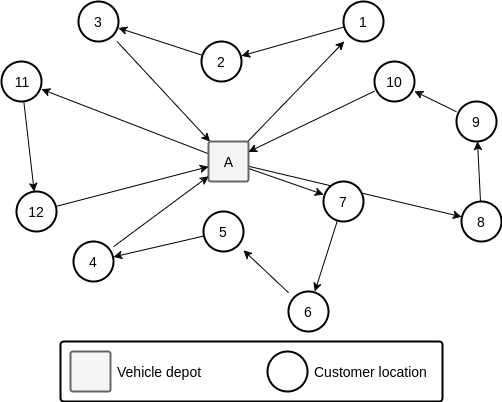
\includegraphics[width=9cm]{Resources/Images/vrp-ilustration}
	\captionsetup{format=hang}
	\caption{Ilustrasi \textit{Vehicle Routing Problem (VRP)}}
	\label{fig:vrp-ilustration}
\end{figure}


Terdapat sejumlah variasi dari VRP klasik yang telah diteliti, antara lain: \textit{Capacitated VRP (CVRP)} yang diteliti oleh \citep{baldacci_exact_2010}, \citep{cordeau_chapter_2007}, dan \citep{toth_vehicle_2002}; \textit{VRP with Time Windows (VRPTW)}, \textit{VRP with Pickup and Delivery (VRPPD)}, dan \textit{Periodic VRP (PVRP)} oleh \citep{solomon_survey_1988}; \textit{Dynamic VRP (DVRP)} oleh \citep{psaraftis_dynamic_1995}, dan berbagai varian lainnya, dimana keseluruhannya hanya mempertimbangkan satu buah depot. Sementara itu, \textit{Multi-Depot Vehicle Routing Problem (MDVRP)} merupakan salah satu varian dari VRP klasik dimana terdapat lebih dari satu \textit{depot} yang digunakan. Gambar \ref{fig:vrp-variants} memberikan ilustrasi hierarki variasi dari VRP.


\begin{figure}[!]
	\centering
	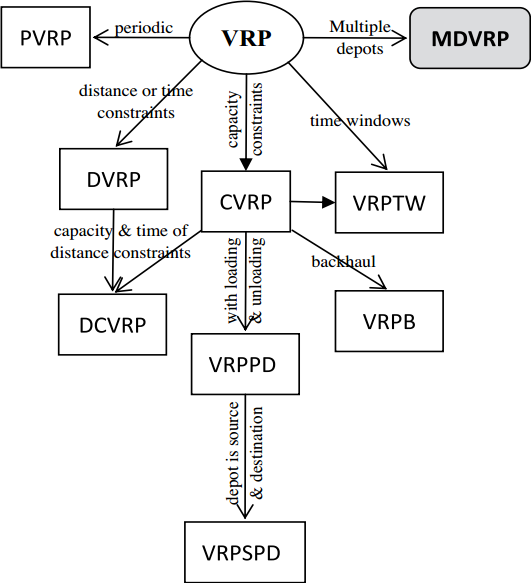
\includegraphics[width=8cm]{Resources/Images/vrp-variants}
	\captionsetup{format=hang}
	\caption{Hierarki variasi dari VRP \citep{weise_solving_2009}}
	\label{fig:vrp-variants}
\end{figure}


%-----------------------------------------------------------------------------%
\subsection{\textit{Multi-Depot Vehicle Routing Problem}}
\label{ssec:mdvrp}
%-----------------------------------------------------------------------------%
\textit{Multi-Depot Vehicle Routing Problem (MDVRP)} merupakan salah satu varian dari VRP klasik dimana terdapat lebih dari satu \textit{depot} yang digunakan. Pada variasi ini, setiap \textit{customer} akan dikunjungi oleh kendaraan yang berasal dari salah satu dari beberapa \textit{depot}. Pada MDVRP standar, kendaraan harus memulai dan mengakhiri rute pada depot yang sama. Gambar \ref{fig:mdvrp-illustration} memberikan ilustrasi tentang MDVRP.


\begin{figure}[!]
	\centering
	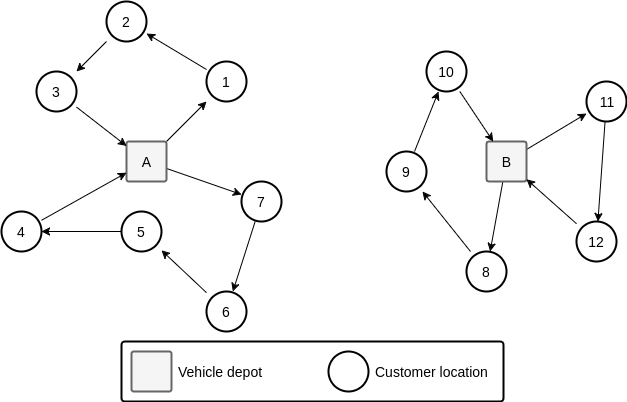
\includegraphics[width=11cm]{Resources/Images/mdvrp-illustration}
	\captionsetup{format=hang}
	\caption{Ilustrasi \textit{Multi Depot} VRP}
	\label{fig:mdvrp-illustration}
\end{figure}


Berdasarkan \citep{renaud_tabu_1996}, MDVRP dapat diformulasikan sebagai berikut, $G = (V, A)$ adalah sebuah \textit{graph}, dimana $V$ adalah sebuah set dari simpul(\textit{vertex} atau \textit{node}) dan $A$ adalah sebuah set dari busur(\textit{arcs}). \textit{Node} dibagi menjadi 2 (dua) \textit{subset}: \textit{customer} yang akan dilayani $V_C$ = \{1,..., $N$\}, dan satu set depot $V_D$ = \{$N$+1,..., $N+M$\}, dimana $V_C \cup V_D$ = $V$ dan $V_C \cap V_D$ = $\oslash$. Terdapat biaya \textit{non-negative} $c_{ij}$ yang diasosiasikan untuk setiap \textit{arc} $(i, j) \in A$. \textit{Demand} untuk masing-masing \textit{customer} adalah $d_i$, dan tidak ada \textit{demand} pada \textit{depot node}. Terdapat juga sejumlah $K$ kendaraan yang identik, yang masing-masing memiliki kapasitas $Q$. \textit{Service time} untuk masing-masing \textit{customer} $i$ adalah $t_i$, sementara waktu durasi maksimum untuk masing-masing rute adalah $T$. Faktor konversi $w_{ij}$ mungkin dibutuhkan untuk menkonversi \textit{cost} $c_{ij}$ menjadi unit waktu. Pada MDVRP klasik, \textit{cost} sama dengan waktu dan unit jarak, sehingga $w_{ij}$ = $1$.


Dalam formula matematika, berdasarkan \citep{kulkarni_integer_1985}, variabel biner $x_{ijk}$ sama dengan $1$ ketika kendaraan $k$ mengunjungi \textit{node} $j$ tepat setelah \textit{node} $i$. Variabel tambahan $y_i$ juga digunakan untuk mengeliminasi \textit{subtour}. Persamaan \ref{eq:1} meminimalisasi \textit{total cost}. Persamaan \ref{eq:2} dan \ref{eq:3} menjamin bahwa setiap \textit{customer} hanya dilayani tepat satu kali oleh satu kendaraan. Alur kendaraan dijamin dengan persamaan \ref{eq:4}. Kapasitas kendaraan dan batasan durasi untuk setiap rute terdapat pada persamaan \ref{eq:5} and \ref{eq:6}. Persamaan \ref{eq:7} dan \ref{eq:8} mengecek keberadaan kendaraan. Eliminasi \textit{subtour} terdapat pada persamaan \ref{eq:9}. Terakhir, persamaan \ref{eq:10} dan \ref{eq:11} mendefinisikan $x$ dan $y$ sebagai variabel biner.


\begin{flalign}
\label{eq:1}
&\sum_{i=1}^{N+M}\sum_{j=1}^{N+M}\sum_{k=1}^{K}c_{ij}x_{ijk};
\end{flalign}


\begin{flalign}
\label{eq:2}
\sum_{i=1}^{N+M}\sum_{k=1}^{K}x_{ijk} = 1  (j=1,..., N);
\end{flalign}


\begin{flalign}
\label{eq:3}
\sum_{j=1}^{N+M}\sum_{k=1}^{K}x_{ijk} = 1  (j=1,..., N);
\end{flalign}


\begin{flalign}
\label{eq:4}
&\sum_{i=1}^{N+M}x_{ihk} - \sum_{j=1}^{N+M}x_{hjk} = 0 \\
\nonumber
&(k=1,...,K; h=1,...,N+M);
\end{flalign}


\begin{flalign}
\label{eq:5}
\sum_{i=1}^{N+M} \sum_{j=1}^{N+M} d_ix_{ijk} \leq Q (k=1,...,K);
\end{flalign}


\begin{flalign}
\label{eq:6}
\sum_{i=1}^{N+M} \sum_{j=1}^{N+M} (c_{ij}w_{ij} + t_i) x_{ijk} \leq T (k=1,...,K);
\end{flalign}


\begin{flalign}
\label{eq:7}
\sum_{i=N+1}^{N+M} \sum_{j=1}^{N} x_{ijk} \leq 1 (k=1,...,K);
\end{flalign}


\begin{flalign}
\label{eq:8}
\sum_{j=N+1}^{N+M} \sum_{i=1}^{N} x_{ijk} \leq 1 (k=1,...,K);
\end{flalign}


\begin{flalign}
\label{eq:9}
&y_i - y_j + (M + N)x_{ijk} \leq N + M - 1; \\
\nonumber
&for 1 \leq i \neq j \leq N and 1 \leq k \leq K;
\end{flalign}


\begin{flalign}
\label{eq:10}
x_{ijk} \in \{0, 1\} \forall i,j,k;
\end{flalign}


\begin{flalign}
\label{eq:11}
y_i \in \{0,1\} \forall i;
\end{flalign}


Terdapat beberapa algoritma yang dapat digunakan untuk menyelesaikan permasalahan MDVRP. \citep{laporte_optimal_1984} dan \citep{laporte_solving_1988} mengembangkan algoritma \textit{branch-and-bound}, tetapi, algoritma ini hanya dapat digunakan untuk sejumlah kecil \textit{instance}. Sejumlah algoritma \textit{heuristic} juga telah diteliti untuk MDVRP. Algoritma heuristic yang relatif awal, yang berbasis pada prosedur \textit{simple construction and improvement} diteliti oleh \citep{tillman_multiple_1969}, \citep{tillman_upperbound_1972}, \citep{tillman_study_1971}, \citep{wren_computer_1972}, \citep{gillett_multi-terminal_1976}, \citep{golden_implementing_1977}, dan \citep{raft_modular_1982}. Penelitian yang lebih baru, \citep{chao_new_1993} mengusulkan sebuah prosedur pencarian yang mengkombinasikan metode lokal \textit{record-to-record} \citep{dueck_new_1993} untuk mengalokasikan ulang pelanggan ke rute kendaraan yang berbeda, yang dilanjutkan dengan prosedur 2-opt \citep{lin_computer_1965} untuk meningkatkan rute individual.


Penelitian yang lain, \citep{renaud_tabu_1996} menggunakan \textit{tabu search heuristic} dimana solusi awal disusun dengan meng-\textit{assign} setiap \textit{customer} dengan depot terdekatnya. Algoritma \textit{petal} yang dirancang oleh penulis yang sama, \citep{renaud_improved_1996}, kemudian digunakan untuk mencari solusi dari setiap VRP yang diasosiasikan pada masing-masing depot. Terakhir terdapat fase \textit{improvement}, baik dengan menggunakan subset dari pertukaran 4-opt untuk meningkatkan rute individual, menukar \textit{customer} antar rute dari depot yang sama maupun berbeda, atau menukar \textit{customer} antara 3 (tiga) rute.


Penggunaan tabu search juga dilakukan oleh \citep{cordeau_tabu_1997}, dimana solusi awal diperoleh dengan meng-assign setiap \textit{customer} dengan depot terdekat dan solusi digenerate untuk masing-masing depot dengan menggunakan algoritma sweep. \textit{Improvement} dilakukan dengan memindahkan \textit{customer} antara dua rute kepada depot yang sama, atau dengan merelokasi \textit{customer} pada rute ke depot yang lain. \textit{Reinsertion} dilakukan dengan menggunakan \textit{GENI heuristic} \citep{gendreau_new_1992}.


Selain tabu search, terdapat juga beberapa algoritma yang dapat digunakan untuk menyelesaikan permasalahan MDVRP, yaitu: adaptive large neighborhood search (ALNS) \citep{pisinger_general_2007}, fuzzy logic guided genetic algorithm (FLGA) \citep{lau_application_2010}, paralel iterated tabu search (ITS) \citep{cordeau_parallel_2012}, hybrid algorithm combining Iterated Local Search and Set Partitioning (ILS-RVND-SP) \citep{subramanian_hybrid_2013}, hybrid genetic algorithm with adaptive diversity control (HGSADC+) \citep{vidal_implicit_2014}, hybrid Granular Tabu Search (ELTG) \citep{escobar_hybrid_2014}, dan evolution algorithms (EAs) \citep{weise_solving_2009}.


%-----------------------------------------------------------------------------%
\subsection{\textit{Cooperative Evolution Strategy}}
\label{ssec:coes}
%-----------------------------------------------------------------------------%
\textit{Evolution Strategies (ESs)} merupakan salah satu \textit{family} dari algoritma optimasi yang terinspirasi dari alam. ESs pertama kali diteliti oleh \citep{rechenberg_cybernetic_1965} dan \citep{huning_evolutionsstrategie._1976}, yang kemudian diteliti lebih lanjut oleh \citep{schwefel_evolutionsstrategie_1975}. Pada ESs, setiap individu direpresentasikan oleh \textit{genetic building blocks} dan parameter strategi yang memodelkan perilaku individu pada lingkungannya. Evolusi kemudian terjadi, yang terdiri dari perkembangan dari karakteristik genetik dan parameter strategi, dimana evolusi dari karakterisik genetik dikontrol oleh parameter strategi.


ESs merepresentasikan individu sebagai sebuah \textit{tuple}, yang terdiri dari \textit{decision vector} $x$ yang akan dioptimalisasi, dan vector parameter strategi $\sigma$ yang merepresentasikan jumlah mutasi dari setiap dimensi.


\begin{flalign}
\chi(t) = (x(t), \sigma(t))
\end{flalign}


Berdasarkan observasi biologi, keturunan (\textit{offspring}) harus mempunyai kesamaan dengan induknya, 


\begin{flalign}
\chi'(t) = (x'(t), \sigma'(t))
\end{flalign}


Operator seleksi kemudian akan menentukan yang terbaik antara induk dan keturunannnya. Asumsi yang digunakan adalah, 


\begin{flalign}
x(t+1) = \left\{\begin{matrix}x'(t) &f(x'(t)) < f(x(t)) \\ 
x(t) &otherwise\end{matrix}\right.
\end{flalign}


dan 


\begin{flalign}
\sigma(t+1) = \left\{\begin{matrix}\sigma'(t) &f(x'(t)) < f(x(t)) \\ 
\sigma(t) &otherwise\end{matrix}\right.
\end{flalign}


Algoritma \ref{alg:es} merupakan framework generik pada implementasi ES. Parameter $\mu$ and $\lambda$ mengindikasikan jumlah induk dan jumlah keturunannya. Komponen utama dari algoritma ES adalah:

\begin{enumerate}
\item \textbf{Initialization:} Untuk setiap individu, \textit{genotype}-nya diinisialisasi sesuai dengan konstrain dari masalah. Parameter dari strategi juga diinisialisasi.
\item \textbf{Recombination:} Keturunan diproduksi dengan melalui operator \textit{crossover} pada dua atau lebih induk.
\item \textbf{Mutation:} Keturunan kemudian bermutasi, dimana jumlah mutasi diukur dari parameter strategi adaptasi.
\item \textbf{Evaluation:} \textit{Absolute fitness function} digunakan untuk mengukur kualitas dari solusi yang direpresentasikan dengan \textit{genotype} dari individu.
\item \textbf{Selection:} Operator seleksi digunakan untuk dua tujuan: memilih induk untuk rekomendasi, dan menentukan individu yang masih bertahan.
\end{enumerate}


\begin{algorithm}[!]
	\captionsetup{format=hang}
	\caption{Algoritma Evolution Strategy}
	\label{alg:es}
	\begin{algorithmic}[1]
		\STATE Set the generation counter, $t = 0$;
		\STATE Initialize the strategy parameters;
		\STATE Create and initialize the population, $C(0)$, of $\mu$ individuals;
		\FOR {each individual, $\chi_i(t) \in C(t)$}
			\STATE Evaluate the fitness, $f(x_i(t))$;
		\ENDFOR
		\WHILE {stopping condition(s) not true}
			\FOR {$i = 1,...,\lambda$}
				\STATE Choose $\rho \geq 2$ parents at random;
				\STATE Create offspring through application of crossover operator on parent genotypes and strategy parameters;
				\STATE Mutate offspring strategy parameters and genotype;
				\STATE Evaluate the fitness of the offspring;
			\ENDFOR
			\STATE Select the new population, $C(t + 1)$;
			\STATE $t = t + 1$;
		\ENDWHILE
	\end{algorithmic}
\end{algorithm}


Jika \textit{evolution algorithm} (EA) memandang evolusi hanya sebagai suatu usaha populasi untuk beradaptasi dengan lingkungan yang tetap, maka algoritma \textit{coevolution} (CoEA) memandang evolusi dari pendekatan yang lebih bersifat natural dengan memperhatikan hubungan yang saling melengkapi (komplemen) antara spesies terkait. Ilustrasi \textit{coevolution} antara dua spesies adalah seperti dicontohkan oleh \citep{holland_echo:_1990}, yaitu interaksi antara tanaman dan serangga. Agar tetap dapat bertahan, tanaman membutuhkan mekanisme evolusi untuk mempertahankan diri dari serangga, sementara serangga membutuhkan tanaman sebagai sumber makanan. Keduanya, tanaman dan serangga, masing-masing berevolusi untuk memdapatkan karakteristik yang membuat mereka bertahan hidup.


Perbedaan antara algoritma CoEA dengan EA adalah CoEA tidak hanya terkait antar populasi, tetapi juga merespon perubahan lingkungan yang disebabkan oleh populasi yang lain. Perbedaan lain yang cukup signifikan adalah EA mendefinisikan solusi optimal melalui fungsi \textit{fitness} yang bersifat absolut yang mendorong terjadinya evolusi. Sebaliknya, CoEA tidak mendefinisikan fungsi \textit{fitness}, sehingga proses evolusi terus berlangsung dimana optimal solusi diperoleh dengan mengalahkan lawan.


Terdapat dua macam pendekatan berbasis \textit{coevolution}, yaitu \textit{competitive coevolution} dan \textit{cooperative coevolution}. \textit{Competitive coevolution} dibagi menjadi dua: 1) \textbf{Competition}, dimana satu atau lebih populasi saling menghambat. Keberhasilan satu populasi membuat populasi lain gagal. 2) \textbf{Amensalism}, dimana terhambatnya satu populasi tidak berpengaruh terhadap populasi lain. Sementara  \textit{cooperative coevolution} juga dibagi menjadi tiga: 1) \textbf{Mutualism}, dimana satu atau lebih populasi saling menguntungkan. 2) \textbf{Commensalism}, dimana hanya sebagian populasi diuntungkan, sementara populasi yang lain tidak terpengaruh. 3) \textbf{Parasitism}, dimana sebagian populasi mengambil keuntungan dari populasi yang lain.


Penelitian yang menggunakan CoEA, dalam kaitannya dengan penyelesaian masalah MDVRP, salah satunya dilakukan oleh \citep{de_oliveira_cooperative_2016}. \citep{de_oliveira_cooperative_2016} membagi masalah menjadi beberapa submasalah, dimana tiap-tiap submasalah akan menjadi sebuah populasi yang akan berinteraksi dengan populasi yang lain. Setiap populasi kemudian akan berevolusi, dimana sebagaimana pada teori \textit{coevolution}, evolusi dari satu populasi akan mempengaruhi populasi yang lain. Pada penelitian \citep{de_oliveira_cooperative_2016}, hubungan yang terjadi pada setiap populasi bersifat \textit{cooperative}, dimana setiap populasi akan bekerja sama membentuk solusi terbaik.


\begin{figure}[!]
	\centering
	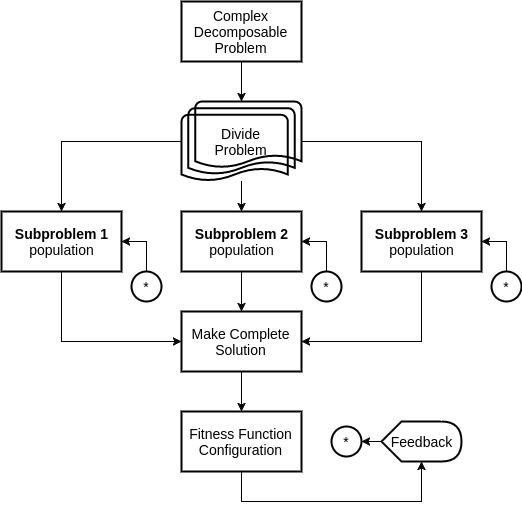
\includegraphics[width=10cm]{Resources/Images/coes_overview}
	\captionsetup{format=hang}
	\caption{\textit{Lifecycle} pada \textit{Cooperative Coevolution} \citep{de_oliveira_cooperative_2016}}
	\label{fig:coes_lifecycle}
\end{figure}


%-----------------------------------------------------------------------------%
\section{Messaging Solution}
\label{sec:messaging-solution}
%-----------------------------------------------------------------------------%


Ketika dua buah aplikasi ingin saling bertukar data, mereka akan melakukannya dengan mengirimkan data melalui \textit{channel} yang akan menghubungkan keduanya. Yang menjadi tantangan adalah memilih \textit{channel} yang tepat dalam pengiriman pesan.


Dari beragam metode interaksi antara \textit{client} dengan \textit{server}, cara yang paling banyak digunakan adalah dengan melalui media web. Hal senada juga terjadi dalam implementasi \textit{location routing problem}, dimana sebagian besar menggunakan media web, seperti \citep{weise_solving_2009}, \citep{sengoku_fast_1998}, \citep{sarmenta_bayanihan_2002}, dan \citep{diaz_vrp_2012}. Akan tetapi, teknologi web bekerja secara \textit{synchronous}, dimana setiap \textit{request} dan \textit{reply} akan diproses secara berurutan, sehingga tidak sesuai untuk diimplementasikan pada sistem yang bersifat \textit{information driven} \citep{muhl_large-scale_2002}. Selain itu, komunikasi \textit{point-to-point} dan \textit{synchronous} membuat pengembangan menjadi tidak fleksibel \citep{eugster_many_2003}.


%-----------------------------------------------------------------------------%
\subsection{Mekanisme \textit{Publish/Subscribe}}
\label{ssec:pub-sub-mechanism}
%-----------------------------------------------------------------------------%
\textit{Publish/subscribe interaction} merupakan salah satu alternatif untuk komunikasi antara \textit{client} dan \textit{server}. Paradigma interaksi pada \textit{publish/subscribe} adalah adanya \textit{subscriber} yang memiliki ketertarikan pada suatu \textit{event} atau \textit{pattern of event} dan ingin mendapatkan notifikasi tiap kali \textit{event} yang menjadi \textit{interest}-nya di-\textit{publish} oleh \textit{publisher}.


Model dasar dari sistem berbasis \textit{publish/subscribe}, seperti Gambar \ref{fig:pub-sub-general}, bergantung pada \textit{event notification service} yang menyediakan penyimpanan dan manajemen dari \textit{subscription}. \textit{Event service} tersebut berperan sebagai mediator antara \textit{publisher} yang berperan sebagai produsen \textit{event} dan \textit{subscriber} yang berperan sebagai konsumen dari \textit{event}. 


\textit{Subscriber} mendaftarkan ketertarikannya pada sebuah \textit{event} tanpa perlu mengetahui sumber dari \textit{event} tersebut, dengan memanggil operasi \textit{subscribe()} pada \textit{event service}. Informasi \textit{subscription} ini tetap tersimpan di dalam penyimpanan pada \textit{event service}. Untuk menciptakan \textit{event}, \textit{publisher} memanggil operasi \textit{publish()}. \textit{Event service} kemudian meneruskan \textit{event} yang diproduksi tersebut kepada \textit{subscriber} yang bersesuaian.


\begin{figure}[!]
	\centering
	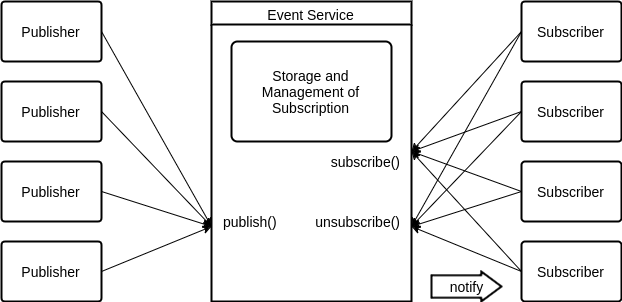
\includegraphics[width=11cm]{Resources/Images/pub-sub-general}
	\captionsetup{format=hang}
	\caption{Arsitektur dasar pada Pub/Sub \citep{eugster_many_2003}}
	\label{fig:pub-sub-general}
\end{figure}


Paradigma \textit{publish/subscribe} memiliki sifat \textit{loose coupling}. Pemisahan (\textit{decoupling}) informasi yang terjadi antara \textit{subscriber} dan \textit{publisher} dapat dibedakan ke dalam 3 (tiga) dimensi, sebagaimana diilustrasikan pada Gambar \ref{fig:space-time-sync-decoupling}. \textit{Decoupling} informasi tersebut berlangsung sebagai berikut:

\begin{enumerate}
\item \textit{Space decoupling.} \\
Interaksi antara \textit{publisher} dan \textit{subscriber} tidak perlu saling mengetahui satu dengan yang lain. \textit{Publisher} mengirimkan \textit{event}, dan \textit{subscriber} menerima \textit{event} secara tidak langsung melalui \textit{event service}. \textit{Publisher} biasanya tidak memiliki referensi tentang \textit{subscriber}. Begitu juga sebaliknya, \textit{subscriber} biasanya tidak memegang referensi tentang \textit{publisher}.
\item \textit{Time decoupling.} \\
Pihak-pihak yang berinteraksi tidak harus berinteraksi pada waktu yang bersamaan. \textit{Publisher} dapat mengirimkan \textit{event} pada saat \textit{subscriber} dalam kondisi terputus (\textit{offline}). Begitu juga sebaliknya, \textit{subscriber} tetap dapat menerima \textit{event}, meskipun \textit{original publisher} sedang dalam kondisi terputus (\textit{offline}).
\item \textit{Synchronizing decoupling.} \\
\textit{Publisher} dan \textit{subscriber} tidak berada dalam \textit{main flow}, sehingga tidak berinteraksi secara \textit{synchronous}. \textit{Publisher} tetap dapat mengirimkan informasi meskipun sedang memproduksi \textit{event} lain dan \textit{subscriber} tetap dapat memperoleh informasi meskipun sedang mengerjakan tugas yang lain. 
\end{enumerate}


\begin{figure}[!]
	\centering
	\begin{subfigure}[t]{9cm}
		\centering
		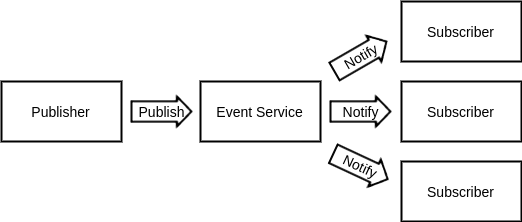
\includegraphics[width=\textwidth]{Resources/Images/space-decoupling}
		\caption{\textit{Space Decoupling}}
		\label{fig:space-decoupling}
	\end{subfigure}%
	
	\begin{subfigure}[t]{10cm}
		\centering
		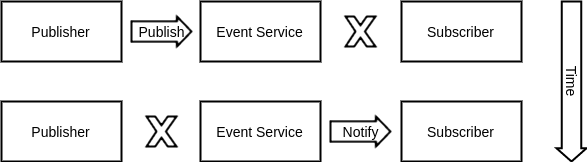
\includegraphics[width=\textwidth]{Resources/Images/time-decoupling}
		\caption{\textit{Time Decoupling}}
		\label{fig:time-decoupling}
	\end{subfigure}%
	
	\begin{subfigure}[t]{9cm}
		\centering
		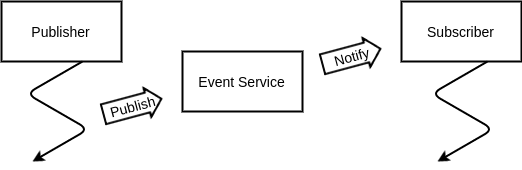
\includegraphics[width=\textwidth]{Resources/Images/sync-decoupling}
		\caption{\textit{Sync Decoupling}}
		\label{fig:sync-decoupling}
	\end{subfigure}
	\captionsetup{format=hang}
	\caption{Pemisahan informasi pada Pub/Sub \citep{eugster_many_2003}}
	\label{fig:space-time-sync-decoupling}
\end{figure}

%-----------------------------------------------------------------------------%
\chapter{\babTiga}
%-----------------------------------------------------------------------------%
%\todo{tambahkan kata-kata pengantar bab 1 disini}


Metodologi penelitian yang akan dilakukan di dalam penelitian ini adalah \textit{Design Science Research Methods and Patterns} \citep{vaishnavi_design_2007}. Metodologi penelitian terdiri dari 5 (lima) tahapan seperti digambarkan pada Gambar \ref{fig:design-science-research-methodology} yaitu: \textit{Awareness of Problem}, \textit{Suggestion}, \textit{Development}, \textit{Evaluation}, dan \textit{Conclusion}.


\begin{figure}[h]
	\centering
	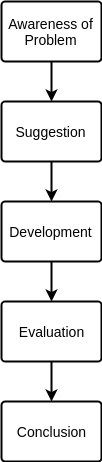
\includegraphics[width=3cm]{Resources/Images/design-science-research-methodology}
	\caption{Tahapan \textit{Design Science Research Methods and Patterns}}
	\label{fig:design-science-research-methodology}
\end{figure}


%-----------------------------------------------------------------------------%
\section{\textit{Awareness of Problem}}
%-----------------------------------------------------------------------------%
Langkah pertama dalam \textit{Design Science Research Methods and Patterns} adalah \textit{awareness of problem}. Langkah ini merupakan proses identifikasi dan definisi masalah. Permasalahan yang diidentifikasi dapat tersusun dari permasalahan nyata (\textit{real problem}) maupun permasalahan penelitian (\textit{research problem}). \textit{Real problem} diidentifikasi melalui analisis dan wawancara dengan \textit{subject matter}. Sementara \textit{research problem} diidentifikasi dari riset-riset yang meneliti permasalahan yang terkait dengan \textit{real problem}.


%-----------------------------------------------------------------------------%
\section{\textit{Suggestion}}
%-----------------------------------------------------------------------------%
Setelah masalah terdefinisikan, maka tahapan berikutnya adalah menemukan solusi dari masalah tersebut. Serangkaian analisis dan \textit{preliminary research} dilakukan untuk menemukan kandidat solusi dari permasalahan. Pada tahapan ini, akan diperoleh keluaran berupa \textit{tentative design} atau \textit{design overview}.


%-----------------------------------------------------------------------------%
\section{\textit{Development}}
%-----------------------------------------------------------------------------%
\textit{Tentative design} yang diperoleh pada tahap sebelumnya kemudian dikembangkan dan diimplementasikan pada tahap ini. Elaborasi dari \textit{tentative design} memerlukan kreatifitas. Complete design diimplementasikan dalam sejumlah bahasa pemrograman yang bervariasi, kemudian dikombinasikan dengan sejumlah software untuk membentuk sebuah prototype sistem. Sebuah mekanisme komunikasi juga dipilih pada tahap ini untuk mendukung implementasi dari sistem.


%-----------------------------------------------------------------------------%
\section{\textit{Evaluation}}
%-----------------------------------------------------------------------------%
Prototype sistem yang diimplementasikan pada tahap sebelumnya kemudian diuji dengan menggunakan serangkaian skenario. Sejumlah data juga digunakan pada tahapan ini. Hasil pengujian kemudian direpresentasikan dalam tabel dan grafik untuk memudahkan dalam menarik kesimpulan.


%-----------------------------------------------------------------------------%
\section{\textit{Conclusion}}
%-----------------------------------------------------------------------------%
Kesimpulan merupakan tahapan akhir dari penelitian. Kesimpulan yang diambil merupakan harus dapat menjawab masalah yang didefinisikan.






%-----------------------------------------------------------------------------%
\chapter{\babEmpat}
%-----------------------------------------------------------------------------%


Bab ini menjelaskan tentang perancangan sistem usulan, yaitu sistem rekomendasi lokasi pencacahan. Sebelum dijelaskan tentang sistem usulan, terlebih dahulu akan dilakukan eksperimen dan analisis terhadap solusi yang telah ada.


%-----------------------------------------------------------------------------%
\section{Analisis}
\label{sec:analysis}
%-----------------------------------------------------------------------------%
Pada kondisi saat ini (sistem berjalan), lokasi pencacahan sudah ditentukan sejak awal dengan menggunakan metode sampling tertentu. Pada tahap perancangan, sejumlah petugas direkrut dan ditugas pada sejumlah lokasi pencacahan. Pengalokasian seringkali dilakukan secara subjektif berdasarkan kedekatan lokasi pencacahan dengan domisili petugas pencacahan. Akibatnya, terjadi ketidakmerataan beban kerja dan variasi total waktu penyelesaian pekerjaan yang sangat tinggi antar petugas. 

Untuk mengatasi masalah ini, algoritma MDVRP dipilih karena memiliki karakteristik yang serupa dengan permasalahan alokasi petugas, yakni: 

\begin{enumerate}
	\item Terdapat lebih dari satu kendaraan. Tiap-tiap kendaraan memiliki depot yang berbeda. Hal ini analog dengan permasalahan alokasi petugas yang melibatkan lebih dari satu pencacah dan tiap-tiap pencacah memiliki titik mulai pencacahan yang berbeda. 
	\item Terdapat biaya yang harus dikeluarkan untuk melakukan perjalanan dari satu pelanggan ke pelanggan yang lain. Ini sejalan dengan konsep dalam pencacahan, yaitu terdapat biaya untuk mengunjungi satu responden ke responden lainnya. 
\end{enumerate}

Pada proses pencacahan, biaya dapat berupa waktu tempuh, jarak tempuh, atau biaya perjalanan. Dalam penelitian ini, waktu tempuh dipilih sebagai representasi dari biaya karena waktu tempuh menggambarkan tingkat kesulitan akses dalam mengunjungi tiap-tiap wilayah kerja. Semakin sulit akses ke suatu wilayah, semakin lama waktu tempuh yang diperlukan. 

Eksperimen dilakukan untuk membuktikan fisibilitas algoritma MDVRP dalam penyelesaian permasalahan alokasi petugas. Eksperimen melibatkan 2 (dua) komponen utama:
\begin{enumerate}
	\item Sejumlah pencacah dengan depotnya masing-masing. 
	\item Sejumlah lokasi pencacahan/blok sensus yang setiap blok sensusnya memiliki beberapa responden. 
\end{enumerate}

\autoref{ssec:mtsp_dataset} hingga \autoref{ssec:hasil-analisis} menyajikan penjelasan rinci mengenai langkah-langkah yang dilakukan dalam eksperimen. 

%-----------------------------------------------------------------------------%
\subsection{Dataset}
\label{ssec:mtsp_dataset}
%-----------------------------------------------------------------------------%
\subsubsection{Lokasi Pencacahan}
%-----------------------------------------------------------------------------%
Merujuk kepada konsep MDVRP, lokasi pencacahan dapat dianalogikan sebagai pelanggan yang akan dikunjungi oleh petugas pencacahan (kendaraan). Pengujian dilakukan dengan menggunakan data 182 lokasi nagari/kelurahan yang bersumber dari data wilayah administratif di Kabupaten Pesisir Selatan, Provinsi Sumatera Barat. Masing-masing lokasi memiliki atribut ID dan posisi koordinat menurut garis lintang dan bujur, seperti yang terlihat pada \autoref{tbl:enumeration_locations}.


\begin{table*}[!]
	\centering
	\ra{1.3}
	\captionsetup{format=hang}
	\caption{Lokasi Pencacahan}
	\label{tbl:enumeration_locations}
	\begin{tabular}{lcc}
		\toprule
		& \multicolumn{2}{c}{Koordinat}\\
		\cmidrule{2-3}
		& Lintang & Bujur\\ 
		\midrule
		1302011001 & -2.3504 & 101.1434\\ 
		1302011002 & -2.4233 & 101.0285\\ 
		1302011003 & -2.3798 & 101.0427\\ 
		1302011004 & -2.3884 & 101.049\\ 
		1302011005 & -2.3936 & 101.0546\\
		...\\
		1302110019 & -1.2387 & 100.4853\\ 
		1302110020 & -1.1408 & 100.4938\\ 
		1302110021 & -1.0883 & 100.4652\\ 
		1302110022 & -1.0886 & 100.489\\ 
		1302110023 & -1.1523 & 100.4978\\
		\bottomrule
	\end{tabular}
\end{table*}


%-----------------------------------------------------------------------------%
\subsubsection{Petugas Pencacahan}
%-----------------------------------------------------------------------------%
Berdasarkan konsep MDVRP, petugas pencacahan diibaratkan sebagai kendaraan yang harus berpindah dari satu lokasi ke lokasi lain secara berurutan. Selain memiliki atribut ID, masing-masing pencacah juga dilengkapi dengan atribut depot, yaitu lokasi di mana pencacah harus memulai dan mengakhiri kunjungan. Eksperimen ini menggunakan 15 pencacah dengan lokasi depot yang bervariasi, seperti contoh yang tercantum pada \autoref{tbl:enumerator}.


\begin{table*}[!]
	\centering
	\ra{1.3}
	\captionsetup{format=hang}
	\caption{Pencacah}
	\label{tbl:enumerator}
	\begin{tabular}{lcc}
		\toprule
		& \multicolumn{2}{c}{Koordinat Depot}\\
		\cmidrule{2-3}
		& Lintang & Bujur\\ 
		\midrule
		1302011008 & -2.3905 & 101.1214\\
		1302012003 & -2.199 & 101.1188\\
		1302020006 & -2.1225 & 101.0687\\
		...\\
		1302100002 & -1.23265 & 100.54314\\
		1302101005 & -1.19831 & 100.58078\\
		1302110003 & -1.2475 & 100.4745\\
		\bottomrule
	\end{tabular}
\end{table*}


%-----------------------------------------------------------------------------%
\subsubsection{Jarak dan Waktu Tempuh}
\label{ss:distance-duration-matrix}
%-----------------------------------------------------------------------------%
Jarak dan waktu tempuh antar lokasi pencacahan digunakan sebagai penimbang dalam penentuan rekomendasi lokasi. Penghitungan jarak dan waktu tempuh dapat dilakukan dengan cara manual (menggunakan hasil survei lokasi dan perkiraan \textit{subject matter}) atau memanfaatkan \textit{Google Directions API} \citep{google_google_2016}. 


Secara teknis, \textit{Google Direction API} lebih unggul dibandingkan metode manual karena secara otomatis memperhitungkan faktor rute tercepat, kondisi geografis, moda transportasi yang digunakan, dan kemacetan lalu lintas dalam memperkirakan jarak dan waktu tempuh. Namun, \textit{Google Direction API} mengandalkan kontribusi para pengguna \textit{Google} sebagai sumber informasi, sehingga ada kemungkinan rute-rute yang jarang dilewati akan memiliki informasi yang minim dan cenderung bias. Sebagai konsekuesinya, terdapat resiko hasil kalkukasi yang kurang tepat untuk rute-rute tersebut. 


Kode \ref{lst:google_direction_api_request} menggambarkan contoh \textit{requests URL} yang dikirimkan ke \textit{Google Direction API}. \textit{Request URL} ini dapat dieksekusi dengan menggunakan \textit{HTTP client}, seperti \textit{curl} dan \textit{wget}, atau \textit{HTTP client library}, seperti \textit{requests} dan \textit{urllib} di Python. Contoh \textit{response} Google Direction API dapat dilihat pada \autoref{fig:google_direction_api_response}.


Hasil kalkulasi jarak dan waktu tempuh kemudian disimpan dalam bentuk matriks seperti yang terlihat pada Tabel \ref{tbl:distance_duration_matrix}. Jika lokasi depot dari pencacah tidak tercakup dalam lokasi pencacahan yang ada, maka lokasi depot tersebut harus ditambahkan ke dalam matriks jarak dan waktu tempuh.


\begin{listing}[!]
	\captionsetup{format=hang}
	\caption{\textit{Google Direction API Request}}
	\label{lst:google_direction_api_request}
	\begin{minted}[showspaces=false, breaklines=true]{http}
https://maps.googleapis.com/maps/api/directions/json?origin=origin_lat,
origin_lon&destination=dest_lat,dest_lon&departure_time=timestamp&
traffic_model=best_guess&key=API_KEY
	\end{minted}
\end{listing}


\begin{figure}[!]
	\centering
	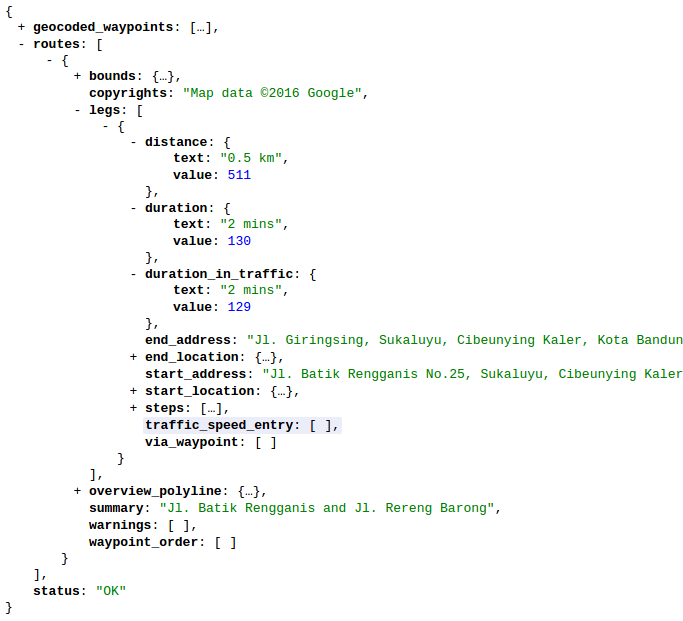
\includegraphics[width=\textwidth]{Resources/Images/google_direction_api_response}
	\captionsetup{format=hang}
	\caption{\textit{Google Direction API Response}}
	\label{fig:google_direction_api_response}
\end{figure}


\begin{table}[!]
	\centering
	\ra{1.3}
	\captionsetup{format=hang}
	\caption{Data Jarak dan Waktu Tempuh}
	\label{tbl:distance_duration_matrix}
	\begin{tabular}{llcc}
		\toprule
		Lokasi A & Lokasi B & Jarak (m) & Waktu Tempuh (det)\\
		\midrule
		1302021001 & 1302021003 & 11119 & 1055\\
		1302021001 & 1302021002 & 9373 & 868\\
		1302021001 & 1302021005 & 490 & 38\\
		1302021001 & 1302021004 & 22760 & 2044\\
		...\\
		1302040015 & 1302012010 & 77889 & 8305\\
		1302040014 & 1302100015 & 103893 & 9984\\
		1302040014 & 1302012010 & 73561 & 7546\\
		1302100015 & 1302012010 & 171636 & 16801\\
		\bottomrule
	\end{tabular}
\end{table}


%-----------------------------------------------------------------------------%
\subsection{Algoritma dan Implementasi}
\label{ssec:alg-impl}
%-----------------------------------------------------------------------------%
Terdapat banyak \textit{library} yang dapat digunakan untuk mengatasi permasalahan MDVRP, baik yang berbayar maupun \textit{open source}. Dua \textit{open source library} yang cukup banyak digunakan untuk menyelesaikan permasalahan MDVRP adalah Jsprit \citep{jsprit_jsprit_2014} dan Optaplanner \citep{optaplanner_constraint_2016}. Eksperimen ini menggunakan JSprit karena JSprit lebih berfokus pada pencarian rute serta lebih mudah untuk diimplementasikan. 


Jsprit merupakan sebuah library berbasis java yang digunakan untuk menyelesaikan permasalahan \textit{traveling salesman problem} (TSP) dan \textit{vehicle routing problems} (VRP). JSprit mencakup berbagai skenario seperti: \textit{pickups and deliveries}, \textit{back hauls}, \textit{heterogeneous fleets}, \textit{finite and infinite fleets}, \textit{multiple depots}, \textit{time windows}, \textit{open routes}, \textit{different start and end locations}, \textit{multiple capacity dimensions}, \textit{initial loads}, dan \textit{skills}. JSpirit bekerja secara terstruktur, mulai dari pendefinisan masalah, pemilihan algoritma, pencarian solusi, hingga pemilihan solusi terbaik.


%-----------------------------------------------------------------------------%
\subsubsection{Definisi Masalah}
%-----------------------------------------------------------------------------%
Pendefinisian masalah dengan \textit{library} Jsprit dilakukan dengan mendefinisikan lokasi pencacahan, para pencacah, dan matriks jarak dan waktu tempuh yang diimplementasikan dalam Kode \ref{lst:jsprit_define_locations}, Kode \ref{lst:jsprit_define_enumerators}, dan Kode \ref{lst:jsprit_define_route_weights}. Ketiga variabel ini kemudian di-\textit{build} menjadi satu dengan menggunakan \textit{syntax} yang tercantum pada Kode \ref{lst:jsprit_build_problem}.


\begin{listing}[!]
	\captionsetup{format=hang}
	\caption{Definisi Lokasi Pencacahan}
	\label{lst:jsprit_define_locations}
	\begin{minted}[showspaces=false,breaklines=true]{java}
Service.Builder builder = Service.Builder.newInstance(line[0]);

try {
	Location loc = Location.Builder.newInstance()
		.setId(line[0])
		.setCoordinate(
	Coordinate.newInstance(Double.parseDouble(line[2]), 
	Double.parseDouble(line[1]))).build();
	builder.setLocation(loc);
} catch (Exception e) {}

Service node = builder.build();
vrpBuilder.addJob(node);
	\end{minted}
\end{listing}


\begin{listing}[!]
	\captionsetup{format=hang}
	\caption{Definisi Pencacah dari File .csv}
	\label{lst:jsprit_define_enumerators}
	\begin{minted}[showspaces=false,breaklines=true]{java}
VehicleTypeImpl.Builder vehicleTypeBuilder = VehicleTypeImpl.Builder.newInstance("enumerator");
vehicleTypeBuilder.setCostPerDistance(0);
vehicleTypeBuilder.setCostPerTransportTime(1);
vehicleTypeBuilder.setCostPerServiceTime(1);
VehicleType vehicleType = vehicleTypeBuilder.build();

VehicleImpl.Builder builder = VehicleImpl.Builder.newInstance(line[0]);

try {
	Location loc = Location.Builder.newInstance()
		.setId(line[0])
		.setCoordinate(Coordinate.newInstance(
			Double.parseDouble(line[2]), Double.parseDouble(line[1])))
		.build();
	builder.setStartLocation(loc);
} catch (Exception e) {}


builder.setType(vehicleType);
VehicleImpl vehicle = builder.build();
vrpBuilder.addVehicle(vehicle);
	\end{minted}
\end{listing}


\begin{listing}[!]
	\captionsetup{format=hang}
	\caption{Definisi Penimbang Jarak dan Waktu Tempuh dari File .csv}
	\label{lst:jsprit_define_route_weights}
	\begin{minted}[showspaces=false,breaklines=true]{java}
VehicleRoutingTransportCostsMatrix.Builder costMatrixBuilder = VehicleRoutingTransportCostsMatrix.Builder.newInstance(true);

while ((line = reader.readNext()) != null) {
	try {
		costMatrixBuilder.addTransportDistance(line[0], line[1], Double.parseDouble(line[2]));
		costMatrixBuilder.addTransportTime(line[0], line[1], Double.parseDouble(line[3]));
	} catch (Exception e) {
		costMatrixBuilder.addTransportDistance(line[0], line[1], 0.0);
		costMatrixBuilder.addTransportTime(line[0], line[1], 0.0);
	}
}

VehicleRoutingTransportCosts costMatrix = costMatrixBuilder.build();
vrpBuilder.setRoutingCost(costMatrix);
	\end{minted}
\end{listing}


\begin{listing}[!]
	\captionsetup{format=hang}
	\caption{Pendefinisian Masalah}
	\label{lst:jsprit_build_problem}
	\begin{minted}[showspaces=false,breaklines=true]{java}
VehicleRoutingProblem.Builder vrpBuilder = VehicleRoutingProblem.Builder.newInstance();
vrpBuilder.setFleetSize(VehicleRoutingProblem.FleetSize.FINITE);
VehicleRoutingProblem problem = vrpBuilder.build();
	\end{minted}
\end{listing}


%-----------------------------------------------------------------------------%
\subsubsection{Konfigurasi Algoritma}
%-----------------------------------------------------------------------------%
Berdasarkan masalah yang telah didefinisikan sebelumnya, JSprit kemudian akan membuat konfigurasi algoritma. Secara \textit{default} algoritma yang digunakan adalah \textit{Tabu Search}. Selain itu, jumlah iterasi dan \textit{thread} yang digunakan juga dapat didefinisikan. Kode \ref{lst:jsprit_create_algorithm} merupakan \textit{syntax} konfigurasi algoritma yang digunakan. 


\begin{listing}[!]
	\captionsetup{format=hang}
	\caption{Penentuan Algoritma}
	\label{lst:jsprit_create_algorithm}
	\begin{minted}[showspaces=false,breaklines=true]{java}
	VehicleRoutingAlgorithm algorithm = Jsprit.Builder.newInstance(problem)
	.setProperty(Jsprit.Parameter.THREADS, 5).buildAlgorithm();
	algorithm.setMaxIterations(iterations);
	\end{minted}
\end{listing}


%-----------------------------------------------------------------------------%
\subsubsection{Pencarian Solusi dan Penentuan Solusi Terbaik}
%-----------------------------------------------------------------------------%
Pencarian solusi dilakukan dengan menggunakan algoritma yang didefinisikan pada tahap sebelumnya. Jika algoritma memproduksi lebih dari satu solusi, maka Jspirit akan melakukan pemilihan solusi terbaik seperti yang terlihat pada Kode \ref{lst:jsprit_search_solution}. Secara \textit{default}, solusi terbaik merupakan solusi yang memiliki total biaya terrendah.


\begin{listing}[!]
	\captionsetup{format=hang}
	\caption{Pencarian Solusi}
	\label{lst:jsprit_search_solution}
	\begin{minted}[showspaces=false,breaklines=true]{java}
	Collection<VehicleRoutingProblemSolution> solutions = algorithm.searchSolutions();
	VehicleRoutingProblemSolution bestSolution = Solutions.bestOf(solutions);
	\end{minted}
\end{listing}


%-----------------------------------------------------------------------------%
\subsection{Hasil dan Analisis}
\label{ssec:hasil-analisis}
%-----------------------------------------------------------------------------%
Berdasarkan hasil dari eksperimen, diperoleh rute seperti yang digambarkan pada Gambar \ref{fig:analysis_mtsp_recommendation} dan Listing \ref{lst:analysis_mtsp_recommendation} untuk detail dari setiap pencacah. Berdasarkan rute tersebut kemudian dilakukan simulasi pencacahan dengan menyertakan waktu tempuh dan lama pencacahan pada tiap-tiap lokasi. Lama pencacahan untuk tiap-tiap lokasi pencacahan dibuat dengan mengikuti distribusi normal. Pengujian dengan menggunakan 182 lokasi pencacahan dan 15 petugas pencacahan menghasilkan rata-rata dan standar deviasi waktu penyelesaian tugas sebesar:  
$$ \mu = 82,24 jam $$
$$ \sigma = 88,95 jam $$


\begin{figure}[!]
	\centering
	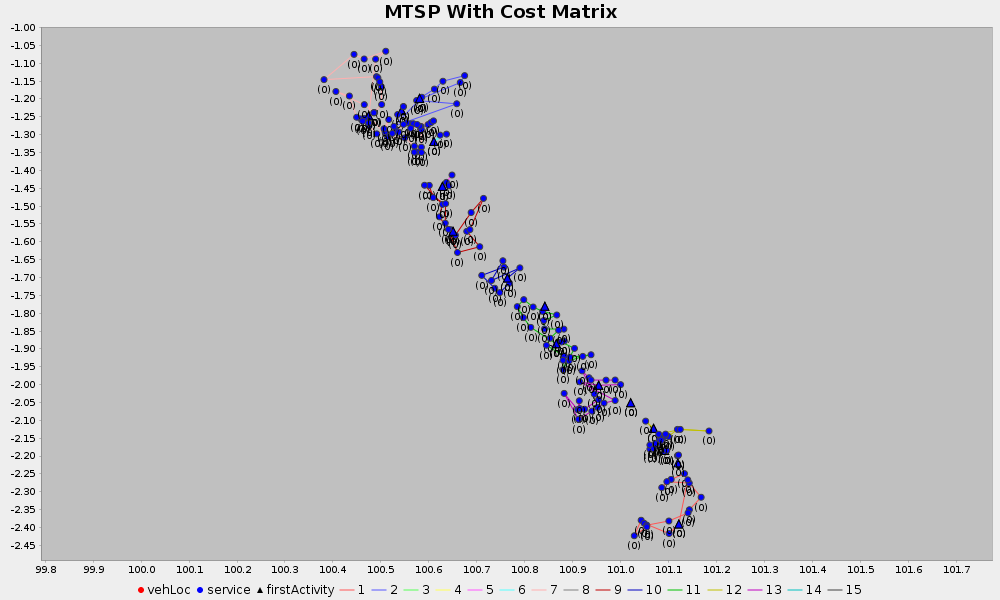
\includegraphics[width=\textwidth]{Resources/Images/analysis_mtsp_no_time_windows}
	\captionsetup{format=hang}
	\caption{Rute yang dihasilkan oleh JSprit}
	\label{fig:analysis_mtsp_recommendation}
\end{figure}


\begin{listing}[!]
	\captionsetup{format=hang}
	\caption{Detail rute yang dihasilkan oleh JSprit}
	\label{lst:analysis_mtsp_recommendation}
	\begin{minted}[showspaces=false,breaklines=true, escapeinside=||]{text}
|\textbf{1302021005}| : 1302021001 --> 1302021005
|\textbf{1302101005}| : 1302101005 --> 1302101001 --> 1302100010 --> 1302100014 --> 1302100011 --> 1302101004 --> 1302101006 --> 1302101003 --> 1302101002
|\textbf{1302070006}| : 1302070006 --> 1302070002 --> 1302070003 --> 1302080009 --> 1302080004 --> 1302080001 --> 1302080005 --> 1302080003 --> 1302070012 --> 1302070011 --> 1302070001 --> 1302070004 --> 1302070007 --> 1302070008 --> 1302070010 --> 1302070009 --> 1302070005
|\textbf{1302050007}| : 1302050007
|\textbf{1302100002}| : 1302100002 --> 1302100003 --> 1302100013 --> 1302100012
|\textbf{1302030005}| : 1302030005
|\textbf{1302110003}| : 1302110003 --> 1302100001 --> 1302090006 --> 1302090012 --> 1302090003 --> 1302090014 --> 1302090009 --> 1302090015 --> 1302090018 --> 1302090016 --> 1302090017 --> 1302090013 --> 1302090005 --> 1302090007 --> 1302090002 --> 1302090008 --> 1302090001 --> 1302100015 --> 1302100004 --> 1302100016 --> 1302090011 --> 1302090010 --> 1302100017 --> 1302100006 --> 1302100007 --> 1302100009 --> 1302100008 --> 1302100005 --> 1302110001 --> 1302110010 --> 1302110013 --> 1302110002 --> 1302110014 --> 1302110015 --> 1302110011 --> 1302110016 --> 1302110017 --> 1302110004 --> 1302110018 --> 1302110019 --> 1302110005 --> 1302110012 --> 1302110023 --> 1302110020 --> 1302110006 --> 1302110007 --> 1302110008 --> 1302110021 --> 1302110009 --> 1302110022
|\textbf{1302012003}| : 1302012007 --> 1302012003 --> 1302012008
|\textbf{1302080006}| : 1302080006 --> 1302080008 --> 1302080002 --> 1302080007
|\textbf{1302031005}| : 1302031005 --> 1302031008 --> 1302030014 --> 1302030006 --> 1302030009 --> 1302030004 --> 1302030010 --> 1302031003 --> 1302030002 --> 1302031004 --> 1302030003 --> 1302030012 --> 1302031001 --> 1302031006 --> 1302040011 --> 1302031009 --> 1302031010 --> 1302031002 --> 1302031007 --> 1302030001
|\textbf{1302060005}| : 1302060005 --> 1302060009 --> 1302060006 --> 1302060008 --> 1302060002 --> 1302060007 --> 1302060001 --> 1302060003 --> 1302060004
|\textbf{1302020006}| : 1302020006 --> 1302020015 --> 1302020011 --> 1302020009 --> 1302020010 --> 1302020001 --> 1302020003 --> 1302020005 --> 1302021006 --> 1302021002 --> 1302021007 --> 1302021008 --> 1302021003 --> 1302021009 --> 1302021004 --> 1302021010 --> 1302020016 --> 1302020017
|\textbf{1302011008}| : 1302011008 --> 1302011007 --> 1302011004 --> 1302011003 --> 1302011002 --> 1302011006 --> 1302011005 --> 1302011009 --> 1302011010 --> 1302011001 --> 1302012005 --> 1302012002 --> 1302012009 --> 1302012010 --> 1302012004 --> 1302012001 --> 1302012006
|\textbf{1302040002}| : 1302040002 --> 1302040003 --> 1302040004 --> 1302040015 --> 1302040008 --> 1302040009 --> 1302040010 --> 1302040014 --> 1302040012 --> 1302040013 --> 1302040001 --> 1302040016 --> 1302040007 --> 1302040006 --> 1302040005 --> 1302050001 --> 1302050004 --> 1302050006 --> 1302050002 --> 1302050008 --> 1302050010 --> 1302050009 --> 1302050005 --> 1302050003
|\textbf{1302090004}| : 1302090004 --> 1302090019 --> 1302090020
	\end{minted}
\end{listing}


\begin{table}[!]
	\centering
	\ra{1.3}
	\captionsetup{format=hang}
	\caption{Waktu total dari setiap rute yang dihasilkan oleh JSprit}
	\label{tbl:enumerators_total_time}
	\begin{tabular}{lc}
		\toprule
		Pencacah & Total Waktu (jam)\\
		\midrule
		1302021005 & 13.3\\
		1302101005 & 60.8\\
		1302070006 & 116\\
		1302050007 & 6\\
		1302100002 & 26.6\\
		1302030005 & 6\\
		1302110003 & 341\\
		1302012003 & 19.9\\
		1302080006 & 27.1\\
		1302031005 & 136\\
		1302060005 & 61.3\\
		1302020006 & 121\\
		1302011008 & 116\\
		1302040002 & 162\\
		1302090004 & 20.2\\
		\bottomrule
	\end{tabular}
\end{table}


Nilai standar deviasi yang tinggi menunjukkan terjadinya ketidakmerataan beban kerja antar pencacah. Ini sekaligus menunjukkan bahwa algoritma MDVRP murni kurang ideal untuk digunakan dalam penentuan rekomendasi. Hal ini terjadi karena algoritma MDVRP memproduksi solusi berupa \textit{precalculated routes} (rute yang harus dikunjungi dari awal hingga akhir tugas pencacahan) tanpa memperhitungkan faktor lamanya waktu kunjungan pada satu lokasi pencacahan. Variabel lama waktu pencacahan hanya akan tersedia jika suatu lokasi sudah selesai dikunjungi sehingga tidak bisa diikutsertakan dalam kalkulasi rekomendasi. \autoref{fig:illustration-timeline-mdvrp-no-service-time} menunjukkan ilustrasi ketidaksesuaian penggunaan algoritma MDVRP murni pada permasalahan alokasi petugas pencacahan yang dapat dijabarkan sebagai berikut:
\begin{enumerate}
	\item Terdapat 10 lokasi pencacahan yang harus dikunjungi. Algoritma MDVRP menciptakan solusi berupa \textit{precalculated routes} untuk petugas A dan B. Tiap-tiap petugas mendapatkan jumlah beban tugas yang sama besar, yakni 5 lokasi. Pada tahap ini, petugas A dan B sama-sama sudah mengetahui urutan lokasi yang akan mereka kunjungi dari awal hingga akhir kegiatan pencacahan. 
	\item Petugas pencacahan A dan B sama-sama memulai tugas pada waktu $t_{s}$ (\textit{time start}) yang digambarkan sebagai segmen berwarna hijau.
	\item Petugas A dan B mengunjungi lokasi pencacahan masing-masing (lokasi \textit{i}) yang memakan waktu selama $t_{i}$ (segmen berwarna putih). Perlu diingat bahwa lokasi $i$ yang dituju oleh petugas A berbeda dengan lokasi $i$ yang dituju oleh petugas B.
	\item Pada setiap lokasi $i$, baik petugas A maupun petugas B memerlukan waktu sebesar $t_{i.1}$ untuk menyelesaikan tugas pencacahan (segmen berwarna biru).  
	\item Petugas A dan B menyelesaikan tugas pada waktu $t_{f}$ (\textit{time finish}) yang digambarkan sebagai segmen berwarna merah muda. 
\end{enumerate}

Dari \autoref{fig:illustration-timeline-mdvrp-no-service-time}, terlihat bahwa kalkulasi rekomendasi rute tanpa melibatkan lama pencacahan mengakibatkan $t_{i}$ dan $t_{i.1}$ yang tidak setara antara petugas A dan B. Hal ini terlihat dari posisi $t_{f}$ petugas A yang jauh berbeda dengan posisi $t_{f}$ petugas B pada \textit{timeline} masing-masing. Petugas A mendapatkan rute dengan rata-rata \textit{service time} ($t_{i.1}$) yang lebih panjang sehingga $t_{f}$ petugas A menjadi lebih besar dibandingkan $t_{f}$ petugas B. Perbedaan yang paling signifikan terlihat pada lokasi pencacahan kedua ($i = 2$), ketika petugas A memiliki $t_{2.1}$ yang hampir 3 (tiga) kali lebih besar dari $t_{2.1}$ petugas B. Sebagai dampaknya, terjadi ketimpangan dalam total waktu penyelesaian pencacahan antar petugas. Beban tugas petugas A menjadi jauh lebih berat dibandingkan petugas B. 

\begin{figure}[!]
	\centering
	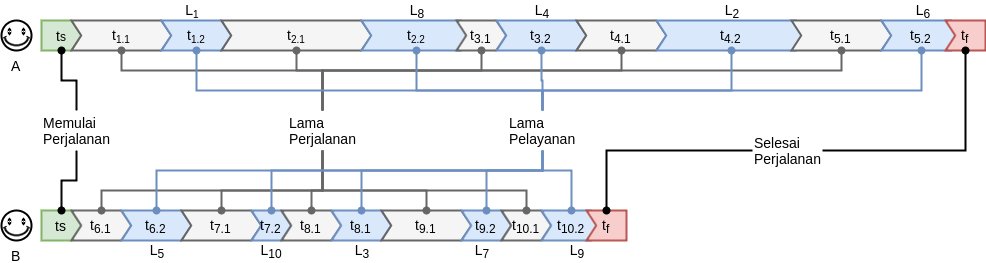
\includegraphics[width=\textwidth]{Resources/Images/illustration-timeline-mdvrp}
	\caption{Ilustrasi \textit{Timeline} Rute yang Dikalkulasi Tanpa Melibatkan Waktu Pencacahan}
	\label{fig:illustration-timeline-mdvrp-no-service-time}
\end{figure}


Untuk mengatasi masalah ini diperlukan suatu mekanisme kalkulasi rekomendasi yang tidak terikat pada lama waktu pencacahan. Mekanisme ini kemudian akan dikombinasikan dengan algoritma MDVRP sehingga menghasilkan suatu metode baru yang dapat menutupi kelemahan MDVRP sekaligus memberikan rekomendasi rute yang lebih adil kepada semua petugas pencacahan. 


%-----------------------------------------------------------------------------%
\section{Perancangan Solusi}
\label{sec:design}
%-----------------------------------------------------------------------------%
Hasil eksperimen pada \autoref{ssec:hasil-analisis} menunjukkan bahwa mekanisme kalkulasi yang bebas dari `lama pencacahan' diperlukan untuk menghilangkan bias dan kesenjangan rute untuk tiap-tiap petugas. Solusi yang diusulkan untuk mengatasi masalah ini adalah dengan melakukan penghitungan rute secara bertahap dengan melakukan `hibridisasi' antara algoritma MDVRP dengan suatu mekanisme \textit{real time}. Idenya adalah, alih-alih menghitung rute secara lengkap diawal pencacahan, lebih baik rute dihitung secara bertahap secara \textit{real time} dengan memanfaatkan `lokasi terkini' dari petugas sebagai depot yang baru pada setiap tahapnya. Pada saat awal pencacahan, petugas hanya mengetahui lokasi pertama yang akan mereka kunjungi. Setelah menyelesaikan tugas pencacahan pada lokasi tersebut, petugas harus mengirimkan permintaan ke \textit{server} guna mengetahui lokasi pencacahan berikutnya.

\autoref{fig:illustration-timeline-realtime-mdvrp} menggambarkan penerapan \textit{real time} MDVRP untuk mengatasi permasalahan alokasi petugas pencacahan yang dijabarkan sebagai berikut:
\begin{enumerate}
	\item Terdapat 10 lokasi pencacahan yang harus dikunjungi. Petugas pencacahan A dan B sama-sama memulai tugas pada waktu $t_{s}$ (segmen berwarna hijau). Berbeda dengan mekanisme pada \autoref{fig:illustration-timeline-mdvrp-no-service-time}, pada tahap ini, petugas A dan B sama-sama tidak memiliki pengetahuan apapun tentang urutan lokasi yang harus mereka kunjungi. 
	\item Pada waktu $t_{1}$ (segmen berwarna kuning), A dan B mengirimkan permintaan ke \textit{server} untuk mendapatkan lokasi pertama yang harus mereka kunjungi. 
	\item A dan B berjalan menuju lokasi pencacahan masing-masing (lokasi \textit{i}) yang memerlukan waktu tempuh sebesar $t_{i.1}$ (segmen berwarna putih). Lokasi $i$ yang dituju oleh petugas A berbeda dengan lokasi $i$ yang dituju oleh petugas B.
	\item A dan B menyelesaikan tugas pencacahan di lokasi pertama yang menghabiskan waktu sebesar $t_{i.2}$ (segmen berwarna biru).
	\item Setelah menyelesaikan tugas di lokasi pertama, A dan B mengirimkan \textit{request} ke server untuk mengetahui lokasi berikutnya yang harus dikunjungi. Server kemudian melakukan rekalkulasi rute dengan melakukan pengecekan terhadap 8 lokasi yang belum dikunjungi dan mencocokkannya dengan `lokasi terkini' dari petugas. Lokasi pencacahan berikutnya yang merupakan lokasi terbaik jika dihitung dari `lokasi terkini', akan dikirimkan sebagai balasan terhadap permintaan yang telah dikirimkan oleh petugas. 
	\item A dan B melanjutkan tugas pencacahan ke lokasi berikutnya (lokasi $i = 2$). Setiap lokasi memerlukan waktu tempuh sebesar $t_{i.1}$ dan waktu penyelesaian pencacahan (\textit{service time}) sebesar $t_{i.2}$. Proses pada poin 2 hingga 6 akan terus berulang hingga seluruh lokasi target pencacahan selesai dikunjungi. 
	\item Petugas A dan B menyelesaikan tugas pada waktu $t_{f}$ (segmen berwarna merah muda) yang hampir sama. Dari \autoref{fig:illustration-timeline-realtime-mdvrp} terlihat bahwa jumlah lokasi yang dikunjungi oleh petugas A lebih sedikit dibandingkan petugas B. Hal ini dikarenakan petugas A memerlukan waktu yang lebih lama untuk melakukan perjalanan ke lokasi serta menyelesaikan tugas pencacahan di lokasi tersebut. 
\end{enumerate}


Mayoritas \textit{real time system} diimplementasikan dengan menggunakan \textit{Web service}. Namun, sistem kerjanya yang \textit{synchronous} (\textit{request} dan \textit{reply} harus diproses secara berurutan) menyebabkan \textit{web service} tidak cocok digunakan untuk aplikasi yang bersifat \textit{information driven} \citep{muhl_large-scale_2002}. Sebagai alternatif, mekanisme \textit{publish/subscribe} dipilih karena memungkinkan terjadinya komunikasi yang \textit{asynchronous} antara \textit{server (publisher)} dan \textit{client (subscriber)}, yaitu komunikasi yang tetap dapat berjalan walaupun salah satu pihak sedang dalam kondisi \textit{offline}.


\begin{figure}[!]
	\centering
	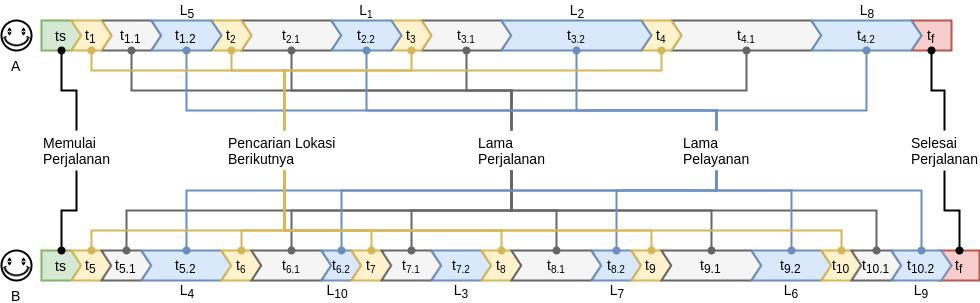
\includegraphics[width=\textwidth]{Resources/Images/illustration-timeline-realtime-mdvrp}
	\captionsetup{format=hang}
	\caption{Ilustrasi \textit{Timeline} Penerapan MDVRP Secara \textit{Real Time}}
	\label{fig:illustration-timeline-realtime-mdvrp}
\end{figure}

%-----------------------------------------------------------------------------%
\subsection{Garis Besar Sistem Usulan}
%-----------------------------------------------------------------------------%
Sistem usulan untuk rekomendasi lokasi pencacahan dirancang berdasarkan arsitektur \textit{publish/subscribe} yang terdiri dari 3 (tiga) komponen utama, yaitu: \textit{publisher} rekomendasi, petugas pencacahan yang berperan sebagai \textit{subscriber}, dan \textit{message broker} yang berperan sebagai penerus pesan (\textit{message router}). \autoref{fig:system-overview} memberikan ilustrasi komponen yang menyusun sistem rekomendasi lokasi pencacahan usulan.


\begin{figure}[!]
	\centering
	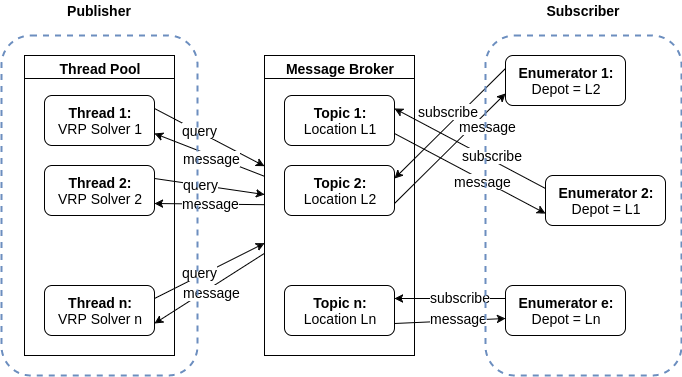
\includegraphics[width=\textwidth]{Resources/Images/system-overview}
	\captionsetup{format=hang}
	\caption{Garis Besar Sistem Usulan}
	\label{fig:system-overview}
\end{figure}


Komunikasi antara \textit{publisher} dan \textit{subscriber} terjadi atas dasar kesamaan topik (\textit{event}). Topik diperoleh dari konteks setiap pencacah yang dapat berupa jenis kelamin, tingkat pendidikan, umur, pengalaman, atau domisili/lokasi pencacah. Pada penelitian ini, `lokasi terkini' dari pencacah dipilih sebagai topik karena bersifat unik, yaitu setiap lokasi pencacahan hanya akan dikunjungi oleh satu orang pencacah saja dan tidak akan ada lebih dari satu pencacah dengan `lokasi terkini' yang sama.


%-----------------------------------------------------------------------------%
\subsection{\textit{Publisher} Rekomendasi}
\label{ssec:publisher}
%-----------------------------------------------------------------------------%
Berdasarkan konsep dasar mekanisme \textit{publish/subscribe}, \textit{publisher} akan mengirimkan informasi ke seluruh \textit{subscriber} tanpa melihat apakah \textit{subscriber} tersebut memang men-\textit{subscribe} topik dari informasi yang bersangkutan atau tidak. Akibatnya informasi yang dikirim banyak yang tidak tepat sasaran sehingga komunikasi yang berlangsung menjadi tidak efisien. Untuk mengatasi inefisiensi komunikasi ini, perlu dilakukan beberapa penyesuaian agar \textit{publisher} hanya akan mengirimkan informasi kepada \textit{subscriber} yang bersesuaian. 

Pada saat seorang petugas pencacahan yang berperan sebagai \textit{subscriber} mengirimkan permintaan `lokasi pencacahan yang harus dituju' kepada \textit{publisher}, permintaan ini tidak langsung diterima oleh \textit{publisher}, melainkan ditampung oleh \textit{message broker}. \textit{Publisher} perlu mengecek \textit{message broker} secara berkala untuk mendeteksi ada atau tidaknya \textit{request} baru dengan menggunakan \textit{thread} $TopicWatcher$ yang dideskripsikan pada \autoref{alg:topic-watcher} serta digambarkan dengan \textit{flowchart} pada \autoref{fig:topic-watcher}. 


\begin{algorithm}[!]
	\captionsetup{format=hang}
	\caption{TopicWatcher}
	\label{alg:topic-watcher}
	\begin{algorithmic}[1]
		\renewcommand{\algorithmicrequire}{\textbf{Input:}}
		\renewcommand{\algorithmicensure}{\textbf{Output:}}
		\REQUIRE $None$
		\ENSURE  $None$
		\\ $TP$ = Threadpool
		\\ $N$ = Number of locations
		\\ $M$ = Number of enumerators
		\WHILE {true}
		\STATE $C \leftarrow readAvailableTopicFromBroker()$	// channel
		\FOR {$m = 1$ to $len(C)$}
		\FOR {$n = 1$ to $N$}
		\IF {($C_m == L_n$)}
		\STATE $T_n = Thread(C_m, E_1...E_M, (unassigned) L_1...L_N)$		// E = enumerator
		\STATE submitThreadToThreadpool($T_n$, $TP$)
		\ENDIF
		\ENDFOR
		\ENDFOR
		\ENDWHILE
	\end{algorithmic}
\end{algorithm}


\begin{figure}[!]
	\centering
	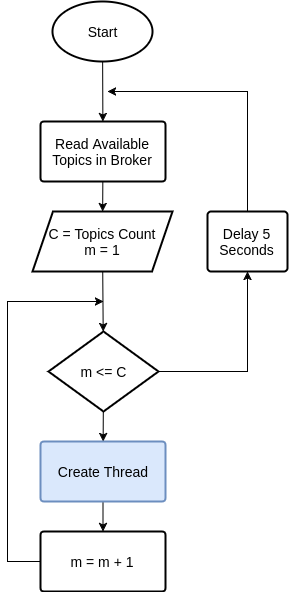
\includegraphics[width=6.3cm]{Resources/Images/topic-watcher}
	\captionsetup{format=hang}
	\caption{\textit{\textit{Flowchart} Topic Watcher}}
	\label{fig:topic-watcher}
\end{figure}


Untuk setiap permintaan yang diterima, \textit{publisher} akan menyiapkan sebuah \textit{thread} baru dengan menggunakan `lokasi terkini' dari \textit{subscriber} (petugas) sebagai ID. \textit{Thread} ini dilengkapi dengan sebuah $VRP solver procedure$ (\autoref{alg:vrp-worker}) yang akan melakukan pencarian solusi/rute. Seluruh \textit{thread} dari masing-masing topik ditampung di dalam sebuah \textit{threadpool} yang menangani \textit{thread} berdasarkan urutan waktu kedatangan. Pada akhir proses pencacahan ketika seluruh lokasi pencacahan telah dialokasikan kepada petugas, ukuran \textit{threadpool} ini akan sama dengan jumlah seluruh topik yang tersedia. 


\textit{Thread-thread} di dalam \textit{threadpool} dieksekusi satu per satu sesuai dengan waktu kedatangan. Setiap eksekusi akan melibatkan \textit{VRPSolver procedure} yang mengikutsertakan $M$ \textit{subscribers} (petugas pencacahan) dan \textit{unassigned} N lokasi pencacahan. \textit{VRPSolver procedure} harus mengikutsertakan seluruh \textit{subscriber} untuk memastikan diperolehnya solusi terbaik yang bersifat global (\textit{global best solution}). \autoref{fig:global-best-greedy-solution} memberikan ilustrasi tentang \textit{Global Best Solution} dengan penjelasan sebagai berikut:
\begin{enumerate}
	\item Petugas A dan B masing-masing melakukan pencacahan pada lokasi 5 dan 6 dan `lokasi terkini' mereka akan diperbarui.
	\item Petugas B menyelesaikan pekerjaannya lebih cepat dari petugas A dan segera mengirimkan permintaan `lokasi pencacahan berikutnya'. Sistem kemudian menghitung dan mengirimkan `lokasi berikutnya' berdasarkan `lokasi terkini' dari petugas B. 
	\item Jika kalkulasi rute hanya melibatkan 1 petugas yang bersangkutan saja, maka \textit{VRPSolver procedure} akan merekomendasikan lokasi terdekat dari `lokasi terkini' petugas B, yakni lokasi 7. Namun, solusi yang dibuat berdasarkan sudut pandang lokal (\textit{local best solution}) seperti ini, dapat `merugikan' petugas lain yang tidak ikut dalam penghitungan. 
	\item Sebagai gambaran, misalkan saat A selesai melakukan pencacahan dan mengirimkan permintaan `lokasi berikutnya', lokasi 7 sudah tidak tersedia lagi bagi A. Rekomendasi terbaik yang bisa diberikan oleh sistem adalah lokasi 1 yang memiliki jarak yang cukup jauh dari A. 
	\item Rekomendasi yang lebih tepat dapat diperoleh jika kalkulasi rute mengikutsertakan seluruh pencacah. Pelibatan terhadap `lokasi terkini' dari seluruh petugas akan menghasilkan solusi yang terbaik dari sudut pandang seluruh pencacah (\textit{global best solution}), sehingga petugas B akan mendapatkan lokasi 3 dan petugas A akan mendapatkan lokasi 7. 

\end{enumerate}

Proses pencarian solusi akan berakhir ketika sudah tidak ada lagi lokasi pencacahan yang berstatus `belum teralokasi'. Adapun \textit{VRP Solver Procedure} dijelaskan secara lebih rinci pada \autoref{ssec:vrp-solver}.


\begin{figure}[!]
	\centering
	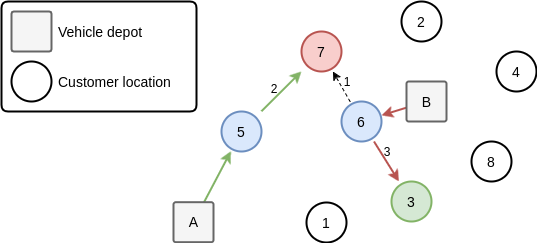
\includegraphics[width=12cm]{Resources/Images/global-best-greedy-solution}
	\captionsetup{format=hang}
	\caption{Ilustrasi \textit{Global Best Solution}}
	\label{fig:global-best-greedy-solution}
\end{figure}


\begin{algorithm}[!]
	\captionsetup{format=hang}
	\caption{\textit{RecommendationPublisher}}
	\label{alg:vrp-worker}
	\begin{algorithmic}[1]
		\renewcommand{\algorithmicrequire}{\textbf{Input:}}
		\renewcommand{\algorithmicensure}{\textbf{Output:}}
		\REQUIRE $TP$		// threadpool
		\ENSURE  $None$
		
		\WHILE {true}
		\STATE $T$ = popFirstThreadOrWaitNewThreadFromThreadpool()
		\STATE $R$ = VRPSolver($T$)
		\FOR {$j = 1$ to $len(R)$}
		\STATE $r$ = publish($C_{R_j}$, $R_j$)
		\IF {($r > 0$)}
		\STATE cancelSolver($T_j$)
		\ELSIF {($C_{T_i} \notin C_{R_j}$)}
		\STATE $T_i = Thread(C_{T_i}, V_m, (unassigned) E_1...E_N)$
		\ENDIF
		\ENDFOR
		\ENDWHILE	
	\end{algorithmic}
\end{algorithm}


Jumlah rute yang dihasilkan oleh \textit{VRPSolver} akan berkisar antara 1 (satu) hingga $M$ rute. $M$ merujuk pada jumlah seluruh petugas pencacahan yang diikutsertakan dalam kalkulasi rute. Setiap rute $R_m$ $(1 \leq m \leq M)$ yang dihasilkan oleh \textit{VRPSolver} akan dikirimkan kepada petugas $m$ yang merupakan \textit{subscriber} topik (lokasi) $C_n$ $(1 \leq n \leq N)$. \textit{Message broker} kemudian akan melaporkan status pengiriman informasi kepada \textit{publisher} (\textit{`success'} atau \textit{`failed'}). Mekanisme kerja \textit{publisher} rekomendasi diilustrasikan dengan menggunakan \textit{flowchart} pada \autoref{fig:recommendation-publisher}.


\begin{figure}[!]
	\centering
	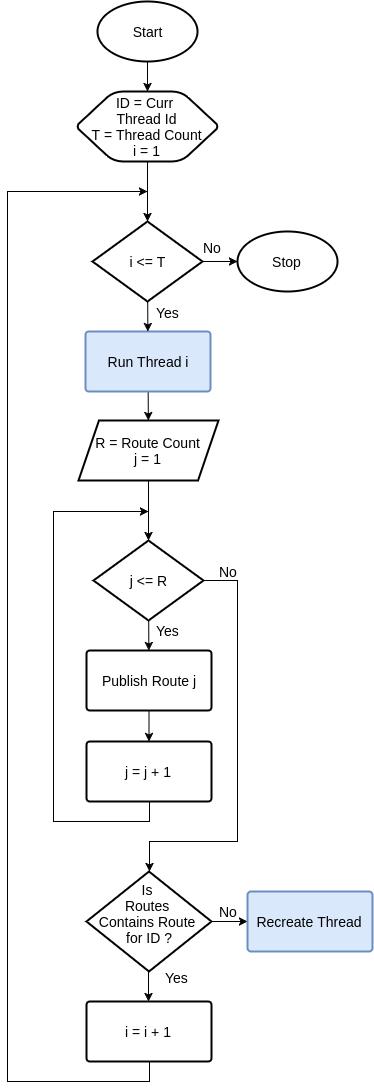
\includegraphics[width=8cm]{Resources/Images/recommendation-publisher}
	\captionsetup{format=hang}
	\caption{\textit{Flowchart recommendation publisher}}
	\label{fig:recommendation-publisher}
\end{figure}


\autoref{fig:timeline-illustration} memberikan gambaran umum tentang proses yang terjadi sejak permintaan lokasi dikirim oleh petugas hingga solusi/rute diperoleh. Petugas B mengirimkan permintaan yang diterima oleh \textit{message broker}. \textit{TopicWatcher} yang memantau \textit{message broker} mengetahui keberadaan permintaan baru ini dan kemudian melaporkannya kepada \textit{publisher}. \textit{Publisher} kemudian menciptakan sebuah \textit{thread} yang mengandung \textit{VRPSolver procedure}. Saat \textit{thread} dieksekusi, \textit{VRPSolver procedure} akan melakukan kalkulasi solusi/rute terbaik dengan mengikutsertakan seluruh $M$ petugas dan lokasi yang masih berstatus \textit{unassigned}. \textit{Thread} hanya dapat dijalankan secara berurutan berdasarkan prinsip `satu dalam satu waktu' (\textit{once at a time}). Sebagai konsekuensinya, ketika petugas A mengirimkan \textit{request} baru, \textit{thread} untuk \textit{request} A tetap akan diciptakan, namun dibiarkan dalam status \textit{idle}. \textit{Thread} A harus menunggu hingga \textit{thread} sebelumnya (\textit{thread} B) selesai diproses. 

Saat \textit{thread} B selesai diproses, \textit{thread} B tidak hanya menghasilkan rute untuk petugas B, tapi juga untuk sejumlah $m$ petugas lainnya ($1 \leq m \leq M$). Rute-rute ini akan dikirimkan kepada petugas yang bersesuaian. Jika suatu rute $R_m$ berhasil diterima oleh petugas $m$, maka \textit{thread} yang berasosiasi dengan rute tersebut akan dihentikan (\textit{terminate}). Dalam \autoref{fig:timeline-illustration}, \textit{thread} B menghasilkan solusi/rute untuk petugas A dan B dan kedua rute ini berhasil diterima dengan baik oleh masing-masing petugas. Dalam hal ini, \textit{thread} A dan \textit{B} dinilai tidak lagi dibutuhkan sehingga kedua \textit{thread} tersebut akan dihentikan. Penghentian ini dilakukan untuk mencegah terjadinya penghitungan ganda terhadap rute yang sudah diterima oleh \textit{subscriber} (petugas). 


\begin{figure}[!]
	\centering
	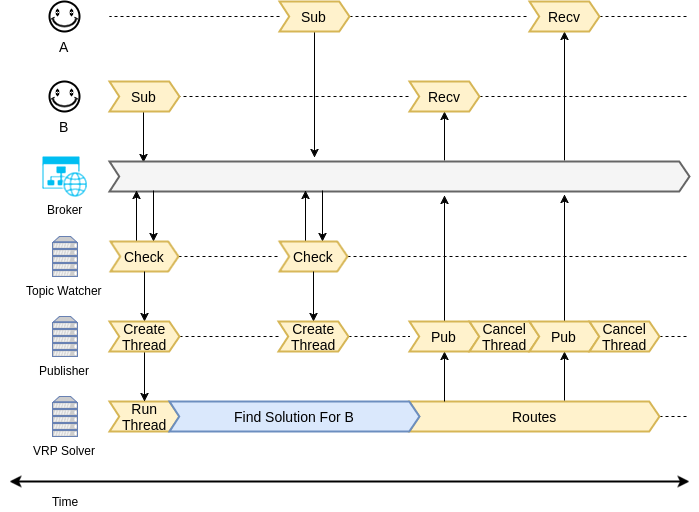
\includegraphics[width=\textwidth]{Resources/Images/timeline-illustration}
	\captionsetup{format=hang}
	\caption{Ilustrasi \textit{Timeline} Proses Pencarian Solusi Berdasarkan}
	\label{fig:timeline-illustration}
\end{figure}


Pada praktiknya, dapat terjadi suatu kondisi ketika \textit{VRPSolver procedure} gagal mendapatkan rute untuk petugas B. Pada kondisi demikian, \textit{thread} B akan diproses ulang dengan hanya melibatkan 1 (satu) petugas B saja dan sejumlah lokasi yang masih berstatus \textit{unassigned}. Ini dilakukan untuk memberikan jaminan bahwa akan selalu ada solusi/rute untuk setiap \textit{request}. 


Pada \autoref{ssec:pub-sub-mechanism} dijelaskan bahwa karakteristik \textit{loose coupling} pada mekanisme \textit{publish/subscribe} membuat \textit{publisher} dan \textit{subscriber} mampu berkomunikasi secara fleksibel, tanpa perlu mengetahui identitas masing-masing. Namun kondisi ini mengakibatkan informasi mengenai `lokasi terkini' dari \textit{subscriber} tidak dapat diperoleh. Untuk mengatasi hal ini, sistem dirancang dengan menyertakan \textit{shared memory} yang dapat digunakan oleh \textit{subscriber} untuk menyimpan \textit{current location}-nya agar kemudian dapat  diakses oleh \textit{publisher}. 


%Proses di atas akan terus berulang sampai seluruh lokasi telah di\textit{assign} kepada \textit{subscriber}. \autoref{fig:publisher-algorithm} mengilustrasikan \textit{workflow} dari algoritma yang digunakan pada \textit{recommendation publisher}.
%
%
%\begin{figure}[!]
%	\centering
%	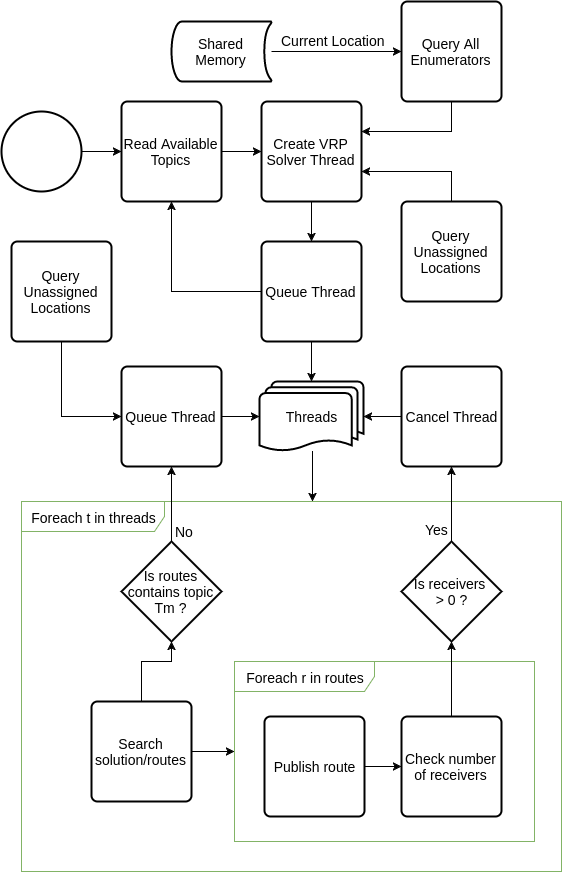
\includegraphics[width=12cm]{Resources/Images/publisher-algorithm}
%	\caption{Publisher Workflow}
%	\label{fig:publisher-algorithm}
%\end{figure}


%-----------------------------------------------------------------------------%
\subsection{\textit{VRP Solver}}
\label{ssec:vrp-solver}
%-----------------------------------------------------------------------------%
\textit{VRP Solver} merupakan sebuah modul yang terdapat di dalam \textit{thread} dan digunakan untuk melakukan kalkulasi rute yang harus dikunjungi oleh petugas. \textit{VRP Solver} dibangun berdasarkan algoritma MDVRP seperti: \textit{tabu search} \cite{cordeau_tabu_1997}, \textit{adaptive large neighborhood search}  \citep{pisinger_general_2007}, \textit{fuzzy logic guided genetic algorithm} \citep{lau_application_2010}, \textit{paralel iterated tabu search} \citep{cordeau_parallel_2012}, \textit{hybrid algorithm combining iterated local search and set partitioning} \citep{subramanian_hybrid_2013}, \textit{hybrid genetic algorithm with adaptive diversity control} \citep{vidal_implicit_2014}, \textit{hybrid granular tabu search} \citep{escobar_hybrid_2014}, dan \textit{cooperative coevolution algorithms} (CoEAs) \citep{de_oliveira_cooperative_2016}. Pada penelitian ini \textit{cooperative coevolutionary algorithms} (CoEAs) dipilih karena menghasilkan rute dengan biaya total yang minimum dan waktu pemrosesan yang relatif singkat dibandingkan algoritma yang lain.


Langkah-langkah yang digunakan dalam implementasi algoritma CoEAs pada \textit{VRPSolver} adalah sebagai berikut:
\begin{enumerate}
\item Definisi masalah \\
Masalah didefinisikan sebagai kumpulan informasi tentang sejumlah $M$ petugas, $N$ lokasi pencacahan, dan $D$ \textit{initial location/depot}. Setiap lokasi $i$, $i \in (D \cup N)$, dilengkapi dengan koordinat lokasi $(x_i, y_i)$. Setiap pasangan lokasi $i$ dan $j$, $i, j \in (D \cup N)$, memiliki biaya sebesar $c_{ij}$ yang merepresentasikan waktu yang diperlukan untuk melakukan perjalanan dari $i$ ke $j$. 

\item Dekomposisi masalah \\
Masalah yang telah didefinisikan sebelumnya akan didekomposisi (dipecah) menjadi beberapa \textit{chunk} submasalah agar proses kalkulasi rute dapat dilakukan secara paralel. 

\item Evolusi \\
Setiap submasalah berisi kombinasi pasangan petugas dan lokasi yang akan dikunjungi (\textit{enumerator-locations pair}). Setiap kombinasi akan mengalami proses evolusi. Pada setiap evolusi yang terjadi, susunan formasi pasangan petugas dan lokasi mengalami perubahan untuk menemukan formasi yang lebih baik. Evolusi terjadi secara iteratif dan setiap iterasi akan menghasilkan formasi baru (\textit{new best formation}). \textit{New best formation} ini akan dievaluasi dengan cara membandingkannya dengan formasi terbaik yang diperoleh dari iterasi sebelumnya (\textit{current best formation}). Jika \textit{new best formation} lebih baik daripada \textit{current best formation}, maka \textit{current best formation} akan diganti dengan \textit{new best formation}. Iterasi akan terus berlangsung sampai dengan solusi/rute yang diperoleh konvergen, yaitu ketika tidak ada lagi \textit{new best formation} yang terbentuk. Formasi yang diperoleh pada akhir keseluruhan iterasi akan dipilih oleh \textit{VRP Solver} sebagai solusi final. 
\end{enumerate}


%-----------------------------------------------------------------------------%
\subsection{\textit{Message Broker}}
\label{ssec:message-broker}
%-----------------------------------------------------------------------------%
\textit{Message broker} merupakan subsistem yang bertanggung jawab dalam menyalurkan (\textit{routing}) pesan dari \textit{publisher} ke \textit{subscriber} dan sebaliknya sesuai dengan topik yang di-\textit{subscribe} \citep{banavar_efficient_1999}. Suatu mekanisme \textit{publish/subscribe} dapat memiliki \textit{single broker} maupun \textit{multi broker}. Pada arsitektur \textit{single broker}, seluruh \textit{subscriber} dan \textit{publisher} terkoneksi pada satu \textit{broker}, sementara pada \textit{multi broker}, \textit{subscriber} maupun \textit{publisher} dapat terkoneksi pada \textit{broker} terdekat. Arsitektur \textit{multi broker} ini disebut juga dengan istilah \textit{distributed publish/subscribe system} \citep{muhl_large-scale_2002}, seperti ilustrasi pada \autoref{fig:pub_sub_distributed_ilustration}. Sistem yang diusulkan akan menerapkan arsitektur terdistribusi agar dapat menangani lokasi pencacahan yang tersebar secara geografis.


\begin{figure}[!]
	\centering
	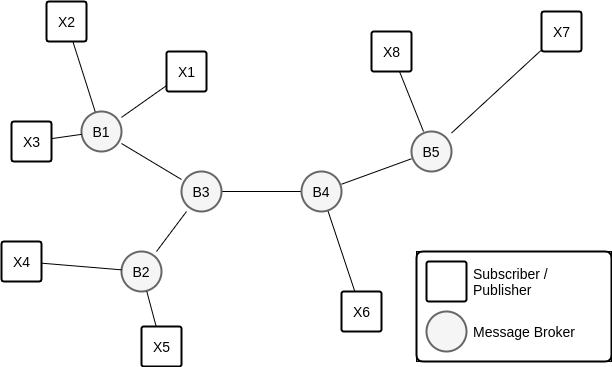
\includegraphics[width=11cm]{Resources/Images/pub_sub_distributed_ilustration}
	\captionsetup{format=hang}
	\caption{Ilustrasi \textit{Publish-Subscribe} terdistribusi}
	\label{fig:pub_sub_distributed_ilustration}
\end{figure}


%#############################################################################%
\begin{comment}
%-----------------------------------------------------------------------------%
\subsection{\textit{Search Algorithm}}
%-----------------------------------------------------------------------------%
Terdapat berbagai variasi algoritma untuk menyelesaikan permasalah TSP maupun VRP, antara lain: genetic algorithm, simmulated annealing, tabu search, particle swarm optimization, harmony search, quantum annealing, greedy 2-opt, dll. Pada pengujian yang dilakukan dengan kasus single-salesman dengan menggunakan 3 (tiga) kriteria: \textit{mean quality}, \textit{dispersion of quality}, dan \textit{time needed to reach the optimum}, simmulated annealing menghasilkan solusi yang paling berkualitas, sementara tabu search merupakan yang paling baik dari sisi performance \citep{antosiewicz_choice_2013}.


%-----------------------------------------------------------------------------%
\subsection{\textit{Greedy Strategy}}
%-----------------------------------------------------------------------------%
Algoritma \textit{greedy} adalah suatu algoritma yang menentukan solusi optimal berdasarkan kondisi saat ini, atau disebut dengan \textit{local optimum}. Algoritma greedy dapat meminimalisir waktu komputasi dalam pencarian solusi global. Pada kasus \textit{travelling salesman problem}, strategi greedy dapat dikatakan dengan "pada setiap tahap, kunjungi kota yang paling dekat dengan lokasi salesman yang belum dikunjungi" \citep{paul_e._black_greedy_2005}. 


Pada metode MTSP, diperoleh lebih dari satu solusi, dimana masing-masing solusi diperbandingkan. Perbandingan dilakukan berdasarkan biaya keseluruhan, dimana solusi dengan biaya terkecil adalah solusi terbaik.


Penentuan solusi terbaik dengan membandingkan biaya keseluruhan tidaklah tepat. \textit{Cost} ditentukan dengan satuan waktu, sementara salah satu komponen utama yang dominan adalah \textit{service time}. Karena \textit{service time} tidak tersedia, maka membandingkan keseluruhan waktu akan menjadi bias. Hipotesis yang ditawarkan adalah membandingkan setiap solusi dengan total biaya untuk lokasi pertama dari masing-masing pencacah saja, karena lokasi pertama tidak terpengaruh dengan \textit{service time}, seperti algoritma dalam Kode \ref{lst:proposed_best_solution_algorithm}.


\begin{listing}
	\caption{Algoritma Solusi Terbaik}
	\label{lst:proposed_best_solution_algorithm}
	\begin{minted}[showspaces=false,breaklines=true]{python}
Let E be all enumerators
Let L be all locations
Run MTSP with enumerators E and locations L
Let S be all solutions from MTSP
Let Cs be an empty dict
For each solution s in S do
	Let R be all routes in solution s
	Let C be 0
	For each route r in R do
		Let J be all jobs in route r
		Let fj be first job in J
		Let cfj be cost of first job fj
		Add C with cjf
	Put C in dict Cs with key solution s
	
Let element in dict Cs with the least value be the best solution
	\end{minted}
\end{listing}


Algoritma \ref{lst:proposed_best_solution_algorithm} merupakan rekomendasi lokasi pertama untuk setiap pencacah. Selanjutnya pencacah dapat melakukan pengumpulan data pada lokasi tersebut sampai selesai, dengan \textit{service time} bervariasi, sehingga waktu selesai pencacahan berbeda-beda antar pencacah. Setiap pencacah yang telah menyelesaikan pengumpulan data, dapat melakukan \textit{subscribe} solusi yang baru kepada \textit{broker}, seperti algoritma pada Kode \ref{lst:proposed_subscribe_solution_algorithm}. Setiap kali broker mendapati adanya \textit{subscribers}, maka \textit{broker} akan mencari solusi baru dengan metode MTSP. Solusi yang dicari hanya menyertakan \textit{subscribers} saja, dan meng-\textit{exclude} lokasi yang telah dikunjungi, seperti algoritma pada Kode \ref{lst:proposed_subscribers_best_solution_algorithm}.


\begin{listing}
	\caption{Algoritma \textit{Subscribe Solution}}
	\label{lst:proposed_subscribe_solution_algorithm}
	\begin{minted}[showspaces=false,breaklines=true]{python}
Let SS be an empty list
For each e in enumerators E do
	If enumerator e has finished enumerating do
		Exclude location l enumerated by e from locations L
		Add e in list of subscribers SS
	\end{minted}
\end{listing}


\begin{listing}
	\caption{Algoritma Solusi Terbaik untuk \textit{Subscribers}}
	\label{lst:proposed_subscribers_best_solution_algorithm}
	\begin{minted}[showspaces=false,breaklines=true]{python}
While locations L is not empty do
	Run MTSP with enumerators SS and locations L
    Let S be all solutions from MTSP
    Let Cs be an empty dict
    For each solution s in S do
	    Let R be all routes in solution s
	    Let C be 0
	    For each route r in R do
		    Let J be all jobs in route r
		    Let fj be first job in J
		    Let cfj be cost of first job fj
		    Add C with cjf
	    Put C in dict Cs with key solution s
	
    Let Bs as element in dict Cs with the least value
    Publish Bs to all subscribers SS
    Set subscribers SS to empty list
	\end{minted}
\end{listing}


%-----------------------------------------------------------------------------%
\subsection{\textit{Publish/Subscribe Paradigm}}
%-----------------------------------------------------------------------------%








\section{Garis Besar Perancangan}

Alur kerja perancangan dimulai dengan dengan mengidentifikasi blok sensus yang akan dilakukan pendataan padanya, serta menentukan jumlah pencacah yang akan digunakan. Kedua permasalahan ini tidak akan dibahas terlalu mendalam dalam penelitian ini. Lokasi pencacahan telah ditentukan dalam fase perancangan sensus dan survei, mengikuti sebuah metodologi tertentu. Sementara jumlah pencacahan juga telah ditentukan, mengikuti jumlah sampel dan berbagai persyaratan tertentu, seperti waktu dan biaya.


Selanjutnya, setiap pencacah akan dialokasikan kepada blok sensus yang akan dicacah dengan menggunakan metode MTSP, sebagaimana diformulasikan oleh \citep{bektas_multiple_2006}, dengan ketentuan setiap pencacah dapat memulai dan mengakhiri pada depot yang berbeda-beda. Setelah model diperoleh, setiap pencacah akan mengunjungi lokasi pertama dari rekomendasi. Setelah selesai kunjungan, lokasi akan disimpan dalam \textit{tabu list} dengan menggunakan metode pub-sub \citep{chen_efficient_2003}. Model baru akan digenerate setiap kali terdapat \textit{request} dari salah satu pencacah. Setiap kali model di-\textit{generate}, \textit{tabu search} \citep{glover_tabu_1989, glover_tabu_1990} yang memanfaatkan \textit{tabu list} akan digunakan untuk memastikan tidak terdapat \textit{conflict}. Setelah model baru selesai di-\textit{generate}, maka mudel akan di-\textit{publish} kepada setiap pencacah yang telah men-\textit{subscribe}.


\begin{figure}[!]
    \centering
    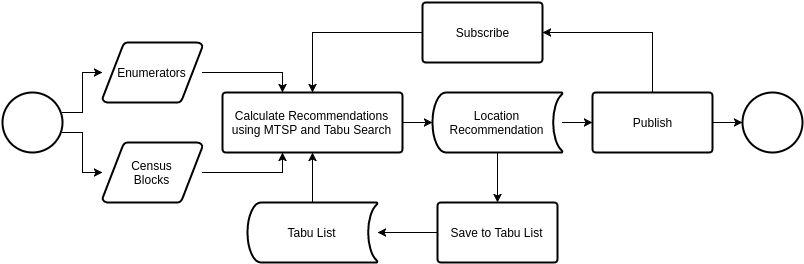
\includegraphics[width=\textwidth]{Resources/Images/design_overview}
    \caption{Garis Besar Sistem Usulan}
    \label{fig:design_overview}
\end{figure}


\section{Penyusunan Rekomendasi}

Pada tahap perumusan rekomendasi, input data yang terdiri dari data pencacah dan data blok sensus akan dioleh menjadi rekomendasi path yang harus dikunjungi. Proses penyusunan rekomendasi menggunakan metode \textit{Multiple Travelling Salesman Problem} (MTSP), yang merupakan pengembangan dari metode klasik \textit{Travelling Salesman Problem} (TSP).


Metode MTSP yang digunakan dalam masalah ini memiliki beberapa \textit{requirements}, antara lain:

\begin{itemize}
\item Jumlah depot \\
MTSP dapat menggunakan lebih dari satu depot, dengan $ m_{j} $ \textit{salesman} untuk setiap depot $ j $. Pada permasalahan ini menggunakan \textit{non-fixed destination}, sehingga pencacahan tidak perlu kembali ke lokasi dimana pencacahan dimulai.
\item Jumlah \textit{salesman} \\
Jumlah \textit{salesman} yang digunakan dapat berupa \textit{fixed number} $ m $, atau dinamis dengan dibatasi jumlah maksimal $ max(m) $. Pada permasalahan ini digunakan \textit{fixed number} $ m $ pencacah.
\item \textit{Fixed charges} \\
Jika jumlah \textit{salesman} dinamis, maka bisa juga masing-masing \textit{salesman} dibatasi dengan sejumlah biaya tertentu. Pada permasalahan ini tidak digunakan \textit{fixed charges}.
\item Waktu kunjungan (\textit{time windows}) \\
\textit{Time windows} merepresentasikan waktu yang dihabiskan selama kunjugan dalam sebuah \textit{node}. Pada kasus ini \textit{time windows} tidak dapat ditentukan karena tidak tersedianya informasi, sehingga dianggap tidak menggunakan \textit{time windows}.
\end{itemize}


Requirements di atas, secara global dapat disederhanakan dalam tabel-tebel berikut. Tabel \ref{tbl:enumerators_overview} menunjukkan rancangan pencacah beserta koordinat depot-nya, sementara Tabel \ref{tbl:census_blocks} menunjukkan rancangan blok sensus beserta koordinat dan \textit{time windows}-nya. Dalam fakta lapangan, jarak antara satu blok sensus dengan blok sensus yang lain tidaklah setara. Bisa jadi secara koordinat memiliki jarak yang berdekatan, tetapi secara akses tidaklah mudah. Untuk itu diperlukan sebuah tabel tambahan, yaitu tabel \textit{cost-matrix}, sebagaimana Tabel \ref{tbl:cost_matrix}. \textit{Cost} yang dimaksud disini adalah segala metrik yang dapat digunakan sebagai penimbang (\textit{weight}), misalnya: biaya, jarak, atau waktu tempuh.


\begin{table}[]
\centering
\caption{Table Pencacah}
\label{tbl:enumerators_overview}
\begin{tabular}{@{}lcc@{}}
\toprule
\multirow{2}{*}{Pencacah} & \multicolumn{2}{l}{\textit{Depot Coordinate}} \\ \cmidrule(l){2-3} 
                          & X                 & Y                \\ \midrule
Pencacah 1                & 20.0              & 20.0             \\
Pencacah 2                & 20.0              & 20.0             \\
Pencacah 3                & 30.0              & 40.0             \\
Pencacah 4                & 30.0              & 40.0             \\
...                       &                   &                  \\
Pencacah m                & x                 & y                \\ \bottomrule
\end{tabular}
\end{table}


\begin{table}[]
\centering
\caption{Tabel Blok Sensus}
\label{tbl:census_blocks}
\begin{tabular}{@{}lccc@{}}
\toprule
\multirow{2}{*}{Blok Sensus} & \multicolumn{2}{c}{Koordinat Lokasi} & \multirow{2}{*}{Time Windows} \\ \cmidrule(lr){2-3}
                             & X                 & Y                &                               \\ \midrule
001B                         & 62.0              & 63.0             & 0                             \\
002B                         & 63.0              & 69.0             & 0                             \\
003B                         & 46.0              & 10.0             & 0                             \\
004B                         & 61.0              & 33.0             & 0                             \\
...                          &                   &                  &                               \\
n                            & x                 & y                & 0                             \\ \bottomrule
\end{tabular}
\end{table}


\begin{table}[]
\centering
\caption{Table \textit{Cost-Matrix}}
\label{tbl:cost_matrix}
\begin{tabular}{@{}|c|c|c|c|c|c|c|@{}}
\toprule
        & 001B & 002B & 003B & 004B & ... & BS ke-n \\ \midrule
001B    & -    & 5    & 2    & 2    &     & ...     \\ \midrule
002B    &      & -    & 4    & 2    &     & ...     \\ \midrule
003B    &      &      & -    & 7    &     & ...     \\ \midrule
004B    &      &      &      & -    &     & ...     \\ \midrule
...     &      &      &      &      & -   & ...     \\ \midrule
BS ke-n &      &      &      &      &     & -       \\ \bottomrule
\end{tabular}
\end{table}


Tabel \textit{cost-matrix}, selain dapat didefinisikan secara manual (berdasarkan hasil survei atau perkiraan \textit{subject matter}), dapat juga didekati dengan menggunakan Google Directions API \citep{google_google_2016}. \textit{Request} yang digunakan menggunakan standar REST API, sementara \textit{response} yang ditampilkan dalam format JSON. Listing \ref{lst:google_direction_api_request} menunjukkan contoh \textit{request}, dan Gambar \ref{fig:google_direction_api_response} menunjukkan contoh \textit{response} dari Google Direction API.








%Gambar \ref{fig:mtsp_solution_example} berikut menunjukkan hasil rekomendasi dengan MTSP.
%
%
%\begin{figure}[!]
%    \centering
%    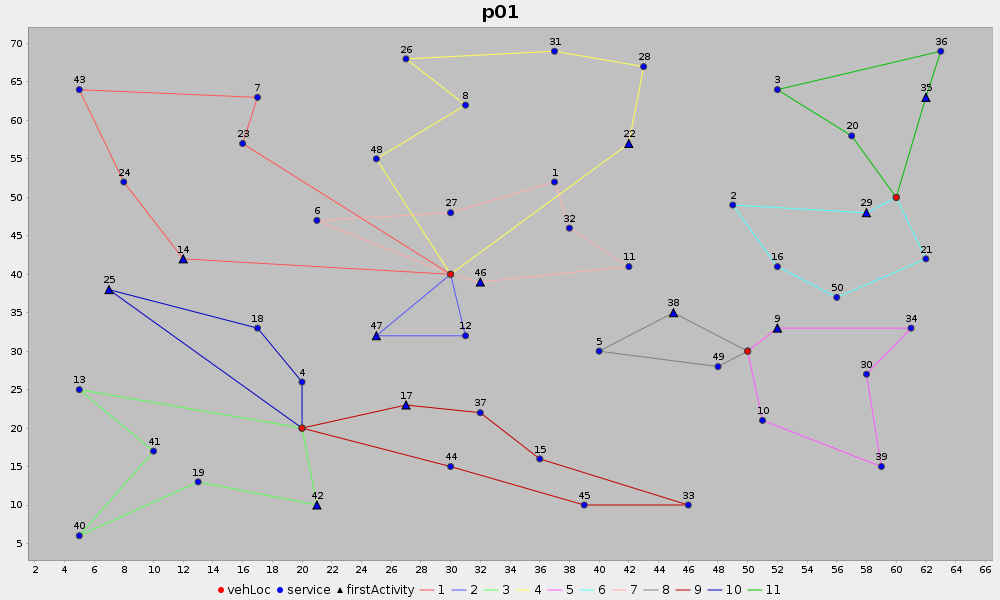
\includegraphics[width=\textwidth]{Resources/Images/mtsp_solution_example}
%    \caption{Contoh Hasil Rekomendasi}
%    \label{fig:mtsp_solution_example}
%\end{figure}


\section{Penyusunan \textit{Conflict Resolution}}


\section{\textit{Publish-Subscribe} Rekomendasi}
\end{comment}
%#############################################################################%

%-----------------------------------------------------------------------------%
\chapter{\babLima}
%-----------------------------------------------------------------------------%
\todo{Tambahkan kata-kata pengantar bab 5 disini.}


%-----------------------------------------------------------------------------%
\section{Mengubah Tampilan Teks}
%-----------------------------------------------------------------------------%
Beberapa perintah yang dapat digunakan untuk mengubah tampilan adalah: 
\begin{itemize}
	\item \bslash f \\
		Merupakan alias untuk perintah \bslash textit, contoh 
		\f{contoh hasil tulisan}.
	\item \bslash bi \\
		\bi{Contoh hasil tulisan}.
	\item \bslash bo \\
		\bo{Contoh hasil tulisan}.
	\item \bslash m \\
		\m{Contoh hasil tulisan}.
	\item \bslash mc \\
		\mc{Contoh hasil tulisan}.
	\item \bslash code \\ 
		\code{Contoh hasil tulisan}.
\end{itemize}


%-----------------------------------------------------------------------------%
\section{Memberikan Catatan}
%-----------------------------------------------------------------------------%
Ada dua perintah untuk memberikan catatan penulisan dalam dokumen yang Anda 
kerjakan, yaitu: 
\begin{itemize}
	\item \bslash todo \\
		Contoh: \\ \todo{Contoh bentuk todo.}
	\item \bslash todoCite \\ 
		Contoh: \todoCite
\end{itemize}


%-----------------------------------------------------------------------------%
\section{Menambah Isi Daftar Isi}
%-----------------------------------------------------------------------------%
Terkadang ada kebutuhan untuk memasukan kata-kata tertentu kedalam Daftar Isi. 
Perintah \bslash addChapter dapat digunakan untuk judul bab dalam Daftar isi. 
Contohnya dapat dilihat pada berkas thesis.tex.


%-----------------------------------------------------------------------------%
\section{Memasukan PDF}
%-----------------------------------------------------------------------------%
Untuk memasukan PDF dapat menggunakan perintah \bslash inpdf yang menerima satu 
buah argumen. Argumen ini berisi nama berkas yang akan digabungkan dalam 
laporan. PDF yang dimasukan degnan cara ini akan memiliki header dan footer 
seperti pada halaman lainnya. 

\inpdf{include}

Cara lain untuk memasukan PDF adalah dengan menggunakan perintah \bslash putpdf 
dengan satu argumen yang berisi nama berkas pdf. Berbeda dengan perintah 
sebelumnya, PDF yang dimasukan dengan cara ini tidak akan memiliki footer atau 
header seperti pada halaman lainnya. 

\putpdf{include}


%-----------------------------------------------------------------------------%
\section{Membuat Perintah Baru}
%-----------------------------------------------------------------------------%
Ada dua perintah yang dapat digunakan untuk membuat perintah baru, yaitu: 
\begin{itemize}
	\item \bslash Var \\
		Digunakan untuk membuat perintah baru, namun setiap kata yang diberikan
		akan diproses dahulu menjadi huruf kapital. 
		Contoh jika perintahnya adalah \bslash Var\{adalah\} makan ketika 
		perintah \bslash Var dipanggil, yang akan muncul adalah ADALAH. 
	\item \bslash var \\
		Digunakan untuk membuat perintah atau baru. 
\end{itemize}


%---------------------------------------------------------------
\chapter{\kesimpulan}
%---------------------------------------------------------------
%\todo{Tambahkan kesimpulan dan saran terkait dengan perkerjaan 
%	yang dilakukan.}


%---------------------------------------------------------------
\section{Kesimpulan}
%---------------------------------------------------------------
Berdasarkan hasil pengujian, diperoleh kesimpulan sebagai berikut:

\begin{enumerate}
	\item Pada permasalahan MDVRP yang tidak mempertimbangkan \textit{service time}, diperoleh hasil bahwasannya sistem usulan yang menggunakan algoritma MDVRP berbasis CoEAs yang dikombinasikan dengan mekanisme Publish/Subscribe menghasilkan total waktu 80 persen lebih buruk dari program pembanding yang menggunakan algoritma MDVRP berbasis CoEAs tanpa mekanisme Publish/Subscribe. Sementara dari sisi \textit{standar deviasi}, sistem usulan menghasilkan 80 persen lebih baik dari aplikasi pembanding. Dengan demikian dapat disimpulkan algoritma MDVRP berbasis CoEAs dengan mekanisme Publish/Subscribe menghasilkan total waktu yang lebih merata antar rute yang dihasilkan, sementara algoritma MDVRP berbasis CoEAs tanpa mekanisme Publish/Subscribe menghasilkan total waktu yang lebih efisien.
	\item Pada permasalahan MDVRP yang mempertimbangkan \textit{service time}, dengan menggunakan data Cordeau PO1 diperoleh hasil total waktu yang dihasilkan dari sistem usulan 6,25 persen lebih buruk dari aplikasi pembanding, tetapi 68,83 persen lebih baik dari sisi standar deviasi. Sementara pada pengujian dengan menggunakan data lapangan, sistem usulan lebih buruk 8,25 persen dibandingkan program pembanding, tetapi 59,11 persen dari sisi standar deviasi. Pada pengujian kondisi normal, dapat disimpulkan algoritma MDVRP berbasis CoEAs dengan mekanisme Publish/Subscribe lebih sesuai digunakan pada permasalahan rekomendasi lokasi pencacahan karena menghasilkan total waktu yang lebih merata antar pencacah.
	\item Pada permasalahan MDVRP yang mempertimbangkan \textit{service time} dan terdapat \textit{delay} dalam jaringan, pada pengujian dengan menggunakan data lapangan diperoleh hasil bahwasannya sistem usulan 4,83 persen lebih buruk dari sisi total waktu, tetapi 3,62 persen lebih baik dari sisi standar deviasi. Pada pengujian kondisi dimana terdapat \textit{delay} pada koneksi, dapat disimpulkan bahwa meskipun memiliki perbedaan yang tipis, algoritma MDVRP berbasis CoEAs dengan mekanisme Publish/Subscribe masih lebih sesuai digunakan pada permasalahan rekomendasi lokasi pencacahan karena menghasilkan total waktu yang lebih merata antar pencacah.
	\item Pada permasalahan MDVRP yang mempertimbangkan \textit{service time} dan terdapat \textit{packet loss} dalam jaringan, pada pengujian dengan menggunakan data lapangan diperoleh hasil bahwasannya sistem usulan 12,79 persen lebih buruk dari sisi total waktu, tetapi 36,14 persen lebih baik dari sisi standar deviasi. Pada pengujian kondisi dimana terdapat \textit{packet loss} pada koneksi, dapat disimpulkan bahwa algoritma MDVRP berbasis CoEAs dengan mekanisme Publish/Subscribe lebih sesuai digunakan pada permasalahan rekomendasi lokasi pencacahan karena menghasilkan total waktu yang lebih merata antar pencacah.
\end{enumerate}


%---------------------------------------------------------------
\section{Saran}
%---------------------------------------------------------------
Dari penelitian ini, saran yang diberikan untuk penelitian selanjutnya sebagai berikut:

\begin{enumerate}
	\item Mengkaji mekanisme komunikasi yang digunakan, misalnya dengan membandingkan dengan mekanisme Request/Reply dan Push/Pull untuk mendapatkan mekanisme komunikasi yang paling tepat.
	\item Mengkaji parameter yang dapat digunakan dalam VRP Solver yaitu lama waktu eksekusi dan lama waktu dimana tidak ada perubahan solusi terbaik, sehingga diperoleh waktu eksekusi yang paling optimal.
	\item Mengkasi penggunaan algoritma MDVRP yang lain, misalnya Tabu Search, Particle Swarm Optimization, dan lain lain, sehingga diperoleh algoritma MDVRP yang paling sesuai.
\end{enumerate}


%
% Daftar Pustaka
%
% Daftar Pustaka 
% 

% 
% Tambahkan pustaka yang digunakan setelah perintah berikut. 
% 
\addcontentsline{toc}{chapter}{\bibname}
\bibliography{\bibFile}



%
% Lampiran 
%
\begin{appendix}
	%
% @author  Andreas Febrian
% @version 1.00 
% 
% Hanya sebuah pembatas bertuliskan LAMPIRAN ditengah halaman. 
% 

\begin{titlepage}
	\centering 
	\vspace*{6cm}
	\noindent \Huge{LAMPIRAN}
	\addChapter{LAMPIRAN}
\end{titlepage}
	
	%-----------------------------------------------------------------------------%
%\addChapter{LAMPIRAN X}
\chapter*{Lampiran A. Hasil Pengujian Kondisi Normal}
\label{ch:lampiran_hasil_pengujian_lapangan_kondisi_normal}
%-----------------------------------------------------------------------------%

\begin{longtable}[!]{c|ccc}
	\captionsetup{format=hang}
	\caption[]{Hasil pengujian kondisi normal pada data lapangan \textit{instance} tw01 dengan menggunakan sistem usulan (algoritma MDVRP berbasis CoEAs dan mekanisme Publish/Subscribe)}
	\label{tbl:test_result_field_tw01}\\
	\toprule
	Pengujian & \MyHead{3.1cm}{Total waktu pencacahan dari seluruh pencacah (hari)} & \MyHead{3.1cm}{Rata-rata waktu pencacahan dari setiap pencacah (hari)} & \MyHead{3.1cm}{Standar deviasi waktu pencacahan dari seluruh pencacah (hari)} \\ 
	\midrule
	\endfirsthead
	\toprule
	\textit{Pengujian} & \MyHead{3.1cm}{Total waktu pencacahan dari seluruh pencacah (hari)} & \MyHead{3.1cm}{Rata-rata waktu pencacahan dari setiap pencacah (hari)} & \MyHead{3.1cm}{Standar deviasi waktu pencacahan dari seluruh pencacah (hari)} \\ 
	\midrule
	\endhead
	\bottomrule
	\endfoot
	1	& 197	& 13	& 1	\\
	2	& 197	& 13	& 2	\\
	3	& 197	& 13	& 1	\\
	4	& 197	& 13	& 1	\\
	5	& 197	& 13	& 2	\\
	6	& 197	& 13	& 2	\\
	7	& 197	& 13	& 1	\\
	8	& 197	& 13	& 1	\\
	9	& 197	& 13	& 1	\\
	10	& 197	& 13	& 2	\\
	11	& 197	& 13	& 2	\\
	12	& 197	& 13	& 1	\\
	13	& 197	& 13	& 1	\\
	14	& 197	& 13	& 1	\\
	15	& 197	& 13	& 2	\\
	16	& 197	& 13	& 2	\\
	17	& 197	& 13	& 2	\\
	18	& 197	& 13	& 1	\\
	19	& 197	& 13	& 2	\\
	20	& 197	& 13	& 2	\\
	21	& 197	& 13	& 2	\\
	22	& 197	& 13	& 2	\\
	23	& 197	& 13	& 2	\\
	24	& 197	& 13	& 1	\\
	25	& 197	& 13	& 1	\\
	26	& 197	& 13	& 2	\\
	27	& 197	& 13	& 1	\\
	28	& 197	& 13	& 2	\\
	29	& 197	& 13	& 2	\\
	30	& 197	& 13	& 1	\\
	31	& 197	& 13	& 2	\\
	32	& 197	& 13	& 2	\\
	33	& 197	& 13	& 3	\\
	34	& 197	& 13	& 2	\\
	35	& 197	& 13	& 1	\\
	36	& 197	& 13	& 2	\\
	37	& 197	& 13	& 2	\\
	38	& 197	& 13	& 1	\\
	39	& 197	& 13	& 2	\\
	40	& 197	& 13	& 1	\\
	41	& 197	& 13	& 2	\\
	42	& 197	& 13	& 1	\\
	43	& 197	& 13	& 2	\\
	44	& 197	& 13	& 2	\\
	45	& 197	& 13	& 1	\\
	46	& 197	& 13	& 1	\\
	47	& 197	& 13	& 2	\\
	48	& 197	& 13	& 1	\\
	49	& 197	& 13	& 1	\\
	50	& 197	& 13	& 2	\\
	51	& 197	& 13	& 1	\\
	52	& 197	& 13	& 1	\\
	53	& 197	& 13	& 1	\\
	54	& 197	& 13	& 2	\\
	55	& 197	& 13	& 1	\\
	56	& 197	& 13	& 1	\\
	57	& 197	& 13	& 2	\\
	58	& 197	& 13	& 2	\\
	59	& 197	& 13	& 1	\\
	60	& 197	& 13	& 2	\\
	61	& 197	& 13	& 1	\\
	62	& 197	& 13	& 1	\\
	63	& 197	& 13	& 2	\\
	64	& 197	& 13	& 2	\\
	65	& 197	& 13	& 1	\\
	66	& 197	& 13	& 1	\\
	67	& 197	& 13	& 1	\\
	68	& 197	& 13	& 2	\\
	69	& 197	& 13	& 1	\\
	70	& 197	& 13	& 2	\\
	71	& 197	& 13	& 2	\\
	72	& 197	& 13	& 3	\\
	73	& 197	& 13	& 1	\\
	74	& 197	& 13	& 1	\\
	75	& 197	& 13	& 2	\\
	76	& 197	& 13	& 2	\\
	77	& 197	& 13	& 1	\\
	78	& 197	& 13	& 2	\\
	79	& 197	& 13	& 1	\\
	80	& 197	& 13	& 2	\\
	81	& 197	& 13	& 1	\\
	82	& 197	& 13	& 3	\\
	83	& 197	& 13	& 2	\\
	84	& 197	& 13	& 2	\\
	85	& 197	& 13	& 1	\\
	86	& 197	& 13	& 2	\\
	87	& 197	& 13	& 1	\\
	88	& 197	& 13	& 2	\\
	89	& 197	& 13	& 2	\\
	90	& 197	& 13	& 2	\\
	91	& 197	& 13	& 1	\\
	92	& 197	& 13	& 2	\\
	93	& 197	& 13	& 2	\\
	94	& 197	& 13	& 2	\\
	95	& 197	& 13	& 1	\\
	96	& 197	& 13	& 1	\\
	97	& 197	& 13	& 1	\\
	98	& 197	& 13	& 1	\\
	99	& 197	& 13	& 1	\\
	100	& 197	& 13	& 2	\\
\end{longtable}


\begin{longtable}[!]{c|ccc}
	\captionsetup{format=hang}
	\caption[]{Hasil pengujian kondisi normal pada data lapangan \textit{instance} tw02 dengan menggunakan sistem usulan (algoritma MDVRP berbasis CoEAs dan mekanisme Publish/Subscribe)}
	\label{tbl:test_result_field_tw02}\\
	\toprule
	Pengujian & \MyHead{3.1cm}{Total waktu pencacahan dari seluruh pencacah (hari)} & \MyHead{3.1cm}{Rata-rata waktu pencacahan dari setiap pencacah (hari)} & \MyHead{3.1cm}{Standar deviasi waktu pencacahan dari seluruh pencacah (hari)} \\ 
	\midrule
	\endfirsthead
	\toprule
	\textit{Pengujian} & \MyHead{3.1cm}{Total waktu pencacahan dari seluruh pencacah (hari)} & \MyHead{3.1cm}{Rata-rata waktu pencacahan dari setiap pencacah (hari)} & \MyHead{3.1cm}{Standar deviasi waktu pencacahan dari seluruh pencacah (hari)} \\ 
	\midrule
	\endhead
	\bottomrule
	\endfoot
	1	& 197	& 13	& 2	\\
	2	& 197	& 13	& 1	\\
	3	& 197	& 13	& 1	\\
	4	& 197	& 13	& 0	\\
	5	& 197	& 13	& 0	\\
	6	& 197	& 13	& 0	\\
	7	& 197	& 13	& 0	\\
	8	& 197	& 13	& 0	\\
	9	& 197	& 13	& 0	\\
	10	& 197	& 13	& 0	\\
	11	& 197	& 13	& 0	\\
	12	& 197	& 13	& 0	\\
	13	& 197	& 13	& 0	\\
	14	& 197	& 13	& 0	\\
	15	& 197	& 13	& 0	\\
	16	& 197	& 13	& 0	\\
	17	& 197	& 13	& 0	\\
	18	& 197	& 13	& 0	\\
	19	& 197	& 13	& 0	\\
	20	& 197	& 13	& 0	\\
	21	& 197	& 13	& 0	\\
	22	& 197	& 13	& 0	\\
	23	& 197	& 13	& 1	\\
	24	& 197	& 13	& 0	\\
	25	& 197	& 13	& 0	\\
	26	& 197	& 13	& 1	\\
	27	& 197	& 13	& 0	\\
	28	& 197	& 13	& 0	\\
	29	& 197	& 13	& 0	\\
	30	& 197	& 13	& 0	\\
	31	& 197	& 13	& 0	\\
	32	& 197	& 13	& 0	\\
	33	& 197	& 13	& 0	\\
	34	& 197	& 13	& 0	\\
	35	& 197	& 13	& 1	\\
	36	& 197	& 13	& 0	\\
	37	& 197	& 13	& 0	\\
	38	& 197	& 13	& 0	\\
	39	& 197	& 13	& 0	\\
	40	& 197	& 13	& 0	\\
	41	& 197	& 13	& 0	\\
	42	& 197	& 13	& 0	\\
	43	& 197	& 13	& 0	\\
	44	& 197	& 13	& 0	\\
	45	& 197	& 13	& 0	\\
	46	& 197	& 13	& 0	\\
	47	& 197	& 13	& 0	\\
	48	& 197	& 13	& 0	\\
	49	& 197	& 13	& 0	\\
	50	& 197	& 13	& 0	\\
	51	& 197	& 13	& 0	\\
	52	& 197	& 13	& 0	\\
	53	& 197	& 13	& 0	\\
	54	& 197	& 13	& 0	\\
	55	& 197	& 13	& 0	\\
	56	& 197	& 13	& 0	\\
	57	& 197	& 13	& 0	\\
	58	& 197	& 13	& 0	\\
	59	& 197	& 13	& 0	\\
	60	& 197	& 13	& 0	\\
	61	& 197	& 13	& 0	\\
	62	& 197	& 13	& 0	\\
	63	& 197	& 13	& 1	\\
	64	& 197	& 13	& 0	\\
	65	& 197	& 13	& 0	\\
	66	& 197	& 13	& 0	\\
	67	& 197	& 13	& 0	\\
	68	& 197	& 13	& 0	\\
	69	& 197	& 13	& 0	\\
	70	& 197	& 13	& 0	\\
	71	& 197	& 13	& 0	\\
	72	& 197	& 13	& 0	\\
	73	& 197	& 13	& 0	\\
	74	& 197	& 13	& 0	\\
	75	& 197	& 13	& 0	\\
	76	& 197	& 13	& 0	\\
	77	& 197	& 13	& 0	\\
	78	& 197	& 13	& 0	\\
	79	& 197	& 13	& 0	\\
	80	& 197	& 13	& 0	\\
	81	& 197	& 13	& 0	\\
	82	& 197	& 13	& 0	\\
	83	& 197	& 13	& 0	\\
	84	& 197	& 13	& 0	\\
	85	& 197	& 13	& 0	\\
	86	& 197	& 13	& 0	\\
	87	& 197	& 13	& 0	\\
	88	& 197	& 13	& 0	\\
	89	& 197	& 13	& 0	\\
	90	& 197	& 13	& 0	\\
	91	& 197	& 13	& 0	\\
	92	& 197	& 13	& 0	\\
	93	& 197	& 13	& 0	\\
	94	& 197	& 13	& 0	\\
	95	& 197	& 13	& 0	\\
	96	& 197	& 13	& 0	\\
	97	& 197	& 13	& 0	\\
	98	& 197	& 13	& 0	\\
	99	& 197	& 13	& 0	\\
	100	& 197	& 13	& 0	\\
\end{longtable}


\begin{longtable}[!]{c|ccc}
	\captionsetup{format=hang}
	\caption[]{Hasil pengujian kondisi normal pada data lapangan \textit{instance} tw03 dengan menggunakan sistem usulan (algoritma MDVRP berbasis CoEAs dan mekanisme Publish/Subscribe)}
	\label{tbl:test_result_field_tw03}\\
	\toprule
	Pengujian & \MyHead{3.1cm}{Total waktu pencacahan dari seluruh pencacah (hari)} & \MyHead{3.1cm}{Rata-rata waktu pencacahan dari setiap pencacah (hari)} & \MyHead{3.1cm}{Standar deviasi waktu pencacahan dari seluruh pencacah (hari)} \\ 
	\midrule
	\endfirsthead
	\toprule
	\textit{Pengujian} & \MyHead{3.1cm}{Total waktu pencacahan dari seluruh pencacah (hari)} & \MyHead{3.1cm}{Rata-rata waktu pencacahan dari setiap pencacah (hari)} & \MyHead{3.1cm}{Standar deviasi waktu pencacahan dari seluruh pencacah (hari)} \\ 
	\midrule
	\endhead
	\bottomrule
	\endfoot
	1	& 197	& 13	& 1	\\
	2	& 197	& 13	& 1	\\
	3	& 197	& 13	& 1	\\
	4	& 197	& 13	& 1	\\
	5	& 197	& 13	& 0	\\
	6	& 197	& 13	& 0	\\
	7	& 197	& 13	& 1	\\
	8	& 197	& 13	& 0	\\
	9	& 197	& 13	& 1	\\
	10	& 197	& 13	& 1	\\
	11	& 197	& 13	& 1	\\
	12	& 197	& 13	& 0	\\
	13	& 197	& 13	& 1	\\
	14	& 197	& 13	& 0	\\
	15	& 197	& 13	& 1	\\
	16	& 197	& 13	& 1	\\
	17	& 197	& 13	& 1	\\
	18	& 197	& 13	& 1	\\
	19	& 197	& 13	& 1	\\
	20	& 197	& 13	& 1	\\
	21	& 197	& 13	& 1	\\
	22	& 197	& 13	& 1	\\
	23	& 197	& 13	& 1	\\
	24	& 197	& 13	& 1	\\
	25	& 197	& 13	& 1	\\
	26	& 197	& 13	& 0	\\
	27	& 197	& 13	& 1	\\
	28	& 197	& 13	& 0	\\
	29	& 197	& 13	& 1	\\
	30	& 197	& 13	& 1	\\
	31	& 197	& 13	& 1	\\
	32	& 197	& 13	& 1	\\
	33	& 197	& 13	& 1	\\
	34	& 197	& 13	& 1	\\
	35	& 197	& 13	& 1	\\
	36	& 197	& 13	& 1	\\
	37	& 197	& 13	& 1	\\
	38	& 197	& 13	& 1	\\
	39	& 197	& 13	& 1	\\
	40	& 197	& 13	& 1	\\
	41	& 197	& 13	& 1	\\
	42	& 197	& 13	& 1	\\
	43	& 197	& 13	& 1	\\
	44	& 197	& 13	& 1	\\
	45	& 197	& 13	& 1	\\
	46	& 197	& 13	& 1	\\
	47	& 197	& 13	& 0	\\
	48	& 197	& 13	& 1	\\
	49	& 197	& 13	& 1	\\
	50	& 197	& 13	& 1	\\
	51	& 197	& 13	& 1	\\
	52	& 197	& 13	& 1	\\
	53	& 197	& 13	& 0	\\
	54	& 197	& 13	& 1	\\
	55	& 197	& 13	& 0	\\
	56	& 197	& 13	& 1	\\
	57	& 197	& 13	& 1	\\
	58	& 197	& 13	& 1	\\
	59	& 197	& 13	& 2	\\
	60	& 197	& 13	& 0	\\
	61	& 197	& 13	& 1	\\
	62	& 197	& 13	& 0	\\
	63	& 197	& 13	& 1	\\
	64	& 197	& 13	& 1	\\
	65	& 197	& 13	& 1	\\
	66	& 197	& 13	& 1	\\
	67	& 197	& 13	& 0	\\
	68	& 197	& 13	& 1	\\
	69	& 197	& 13	& 1	\\
	70	& 197	& 13	& 0	\\
	71	& 197	& 13	& 1	\\
	72	& 197	& 13	& 1	\\
	73	& 197	& 13	& 1	\\
	74	& 197	& 13	& 0	\\
	75	& 197	& 13	& 1	\\
	76	& 197	& 13	& 1	\\
	77	& 197	& 13	& 1	\\
	78	& 197	& 13	& 0	\\
	79	& 197	& 13	& 1	\\
	80	& 197	& 13	& 1	\\
	81	& 197	& 13	& 1	\\
	82	& 197	& 13	& 1	\\
	83	& 197	& 13	& 1	\\
	84	& 197	& 13	& 1	\\
	85	& 197	& 13	& 0	\\
	86	& 197	& 13	& 1	\\
	87	& 197	& 13	& 1	\\
	88	& 197	& 13	& 1	\\
	89	& 197	& 13	& 1	\\
	90	& 197	& 13	& 1	\\
	91	& 197	& 13	& 1	\\
	92	& 197	& 13	& 1	\\
	93	& 197	& 13	& 1	\\
	94	& 197	& 13	& 1	\\
	95	& 197	& 13	& 1	\\
	96	& 197	& 13	& 1	\\
	97	& 197	& 13	& 1	\\
	98	& 197	& 13	& 0	\\
	99	& 197	& 13	& 1	\\
	100	& 197	& 13	& 1	\\
\end{longtable}


\begin{longtable}[!]{c|ccc}
	\captionsetup{format=hang}
	\caption[]{Hasil pengujian kondisi normal pada data lapangan \textit{instance} tw04 dengan menggunakan sistem usulan (algoritma MDVRP berbasis CoEAs dan mekanisme Publish/Subscribe)}
	\label{tbl:test_result_field_tw04}\\
	\toprule
	Pengujian & \MyHead{3.1cm}{Total waktu pencacahan dari seluruh pencacah (hari)} & \MyHead{3.1cm}{Rata-rata waktu pencacahan dari setiap pencacah (hari)} & \MyHead{3.1cm}{Standar deviasi waktu pencacahan dari seluruh pencacah (hari)} \\ 
	\midrule
	\endfirsthead
	\toprule
	\textit{Pengujian} & \MyHead{3.1cm}{Total waktu pencacahan dari seluruh pencacah (hari)} & \MyHead{3.1cm}{Rata-rata waktu pencacahan dari setiap pencacah (hari)} & \MyHead{3.1cm}{Standar deviasi waktu pencacahan dari seluruh pencacah (hari)} \\ 
	\midrule
	\endhead
	\bottomrule
	\endfoot
	1	& 197	& 13	& 0	\\
	2	& 197	& 13	& 0	\\
	3	& 197	& 13	& 1	\\
	4	& 197	& 13	& 0	\\
	5	& 197	& 13	& 0	\\
	6	& 197	& 13	& 0	\\
	7	& 197	& 13	& 0	\\
	8	& 197	& 13	& 0	\\
	9	& 197	& 13	& 1	\\
	10	& 197	& 13	& 0	\\
	11	& 197	& 13	& 0	\\
	12	& 197	& 13	& 0	\\
	13	& 197	& 13	& 0	\\
	14	& 197	& 13	& 0	\\
	15	& 197	& 13	& 0	\\
	16	& 197	& 13	& 0	\\
	17	& 197	& 13	& 0	\\
	18	& 197	& 13	& 0	\\
	19	& 197	& 13	& 0	\\
	20	& 197	& 13	& 0	\\
	21	& 197	& 13	& 0	\\
	22	& 197	& 13	& 1	\\
	23	& 197	& 13	& 0	\\
	24	& 197	& 13	& 0	\\
	25	& 197	& 13	& 1	\\
	26	& 197	& 13	& 0	\\
	27	& 197	& 13	& 0	\\
	28	& 197	& 13	& 0	\\
	29	& 197	& 13	& 0	\\
	30	& 197	& 13	& 0	\\
	31	& 197	& 13	& 0	\\
	32	& 197	& 13	& 0	\\
	33	& 197	& 13	& 0	\\
	34	& 197	& 13	& 0	\\
	35	& 197	& 13	& 0	\\
	36	& 197	& 13	& 0	\\
	37	& 197	& 13	& 0	\\
	38	& 197	& 13	& 0	\\
	39	& 197	& 13	& 0	\\
	40	& 197	& 13	& 0	\\
	41	& 197	& 13	& 0	\\
	42	& 197	& 13	& 0	\\
	43	& 197	& 13	& 0	\\
	44	& 197	& 13	& 0	\\
	45	& 197	& 13	& 0	\\
	46	& 197	& 13	& 0	\\
	47	& 197	& 13	& 0	\\
	48	& 197	& 13	& 0	\\
	49	& 197	& 13	& 0	\\
	50	& 197	& 13	& 0	\\
	51	& 197	& 13	& 0	\\
	52	& 197	& 13	& 0	\\
	53	& 197	& 13	& 0	\\
	54	& 197	& 13	& 0	\\
	55	& 197	& 13	& 0	\\
	56	& 197	& 13	& 0	\\
	57	& 197	& 13	& 0	\\
	58	& 197	& 13	& 0	\\
	59	& 197	& 13	& 0	\\
	60	& 197	& 13	& 0	\\
	61	& 197	& 13	& 0	\\
	62	& 197	& 13	& 0	\\
	63	& 197	& 13	& 0	\\
	64	& 197	& 13	& 0	\\
	65	& 197	& 13	& 0	\\
	66	& 197	& 13	& 0	\\
	67	& 197	& 13	& 0	\\
	68	& 197	& 13	& 0	\\
	69	& 197	& 13	& 0	\\
	70	& 197	& 13	& 0	\\
	71	& 197	& 13	& 0	\\
	72	& 197	& 13	& 0	\\
	73	& 197	& 13	& 0	\\
	74	& 197	& 13	& 0	\\
	75	& 197	& 13	& 0	\\
	76	& 197	& 13	& 0	\\
	77	& 197	& 13	& 0	\\
	78	& 197	& 13	& 0	\\
	79	& 197	& 13	& 0	\\
	80	& 197	& 13	& 0	\\
	81	& 197	& 13	& 0	\\
	82	& 197	& 13	& 0	\\
	83	& 197	& 13	& 0	\\
	84	& 197	& 13	& 0	\\
	85	& 197	& 13	& 0	\\
	86	& 197	& 13	& 0	\\
	87	& 197	& 13	& 0	\\
	88	& 197	& 13	& 0	\\
	89	& 197	& 13	& 0	\\
	90	& 197	& 13	& 0	\\
	91	& 197	& 13	& 0	\\
	92	& 197	& 13	& 0	\\
	93	& 197	& 13	& 0	\\
	94	& 197	& 13	& 0	\\
	95	& 197	& 13	& 0	\\
	96	& 197	& 13	& 0	\\
	97	& 197	& 13	& 0	\\
	98	& 197	& 13	& 0	\\
	99	& 197	& 13	& 0	\\
	100	& 197	& 13	& 0	\\
\end{longtable}
	%-----------------------------------------------------------------------------%
\addChapter{LAMPIRAN X}
\chapter*{Lampiran X}
\label{ch:lampiran_hasil_pengujian_kondisi_delay}
%-----------------------------------------------------------------------------%


\begin{longtable}[!]{c|ccc}
	\caption{Hasil pengujian kondisi \textit{delay} pada data lapangan \textit{instance} d01 dengan menggunakan sistem usulan (algoritma MDVRP berbasis CoEAs dan mekanisme Publish/Subscribe)}
	\label{tbl:test_result_d01_tw}\\
	\toprule
	Pengujian & \MyHead{3.1cm}{Total waktu pencacahan dari seluruh pencacah (hari)} & \MyHead{3.1cm}{Rata-rata waktu pencacahan dari setiap pencacah (hari)} & \MyHead{3.1cm}{Standar deviasi waktu pencacahan dari seluruh pencacah (hari)} \\ 
	\midrule
	\endfirsthead
	\toprule
	\textit{Pengujian} & \MyHead{3.1cm}{Total waktu pencacahan dari seluruh pencacah (hari)} & \MyHead{3.1cm}{Rata-rata waktu pencacahan dari setiap pencacah (hari)} & \MyHead{3.1cm}{Standar deviasi waktu pencacahan dari seluruh pencacah (hari)} \\ 
	\midrule
	\endhead
	\bottomrule
	\endfoot
	1	& 223	& 14	& 3	\\
	2	& 221	& 14	& 2	\\
	3	& 219	& 14	& 3	\\
	4	& 223	& 14	& 1	\\
	5	& 230	& 15	& 1	\\
	6	& 223	& 14	& 1	\\
	7	& 222	& 14	& 1	\\
	8	& 227	& 15	& 1	\\
	9	& 229	& 15	& 1	\\
	10	& 221	& 14	& 1	\\
	11	& 224	& 14	& 2	\\
	12	& 215	& 14	& 1	\\
	13	& 234	& 15	& 1	\\
	14	& 220	& 14	& 1	\\
	15	& 217	& 14	& 1	\\
	16	& 229	& 15	& 1	\\
	17	& 219	& 14	& 1	\\
	18	& 226	& 15	& 1	\\
	19	& 233	& 15	& 1	\\
	20	& 219	& 14	& 1	\\
	21	& 218	& 14	& 1	\\
	22	& 220	& 14	& 1	\\
	23	& 215	& 14	& 1	\\
	24	& 220	& 14	& 1	\\
	25	& 220	& 14	& 1	\\
	26	& 218	& 14	& 1	\\
	27	& 221	& 14	& 1	\\
	28	& 224	& 14	& 1	\\
	29	& 217	& 14	& 1	\\
	30	& 227	& 15	& 1	\\
	31	& 222	& 14	& 1	\\
	32	& 226	& 15	& 1	\\
	33	& 234	& 15	& 2	\\
	34	& 219	& 14	& 1	\\
	35	& 224	& 14	& 1	\\
	36	& 229	& 15	& 1	\\
	37	& 224	& 14	& 1	\\
	38	& 222	& 14	& 1	\\
	39	& 224	& 14	& 2	\\
	40	& 218	& 14	& 1	\\
	41	& 224	& 14	& 1	\\
	42	& 221	& 14	& 1	\\
	43	& 235	& 15	& 1	\\
	44	& 223	& 14	& 1	\\
	45	& 218	& 14	& 1	\\
	46	& 234	& 15	& 1	\\
	47	& 217	& 14	& 1	\\
	48	& 224	& 14	& 1	\\
	49	& 224	& 14	& 1	\\
	50	& 219	& 14	& 1	\\
	51	& 223	& 14	& 1	\\
	52	& 221	& 14	& 1	\\
	53	& 227	& 15	& 1	\\
	54	& 221	& 14	& 1	\\
	55	& 222	& 14	& 1	\\
	56	& 226	& 15	& 1	\\
	57	& 224	& 14	& 1	\\
	58	& 223	& 14	& 1	\\
	59	& 231	& 15	& 1	\\
	60	& 220	& 14	& 1	\\
	61	& 221	& 14	& 1	\\
	62	& 228	& 15	& 1	\\
	63	& 217	& 14	& 1	\\
	64	& 226	& 15	& 1	\\
	65	& 227	& 15	& 1	\\
	66	& 225	& 15	& 1	\\
	67	& 224	& 14	& 1	\\
	68	& 225	& 15	& 2	\\
	69	& 227	& 15	& 1	\\
	70	& 223	& 14	& 1	\\
	71	& 234	& 15	& 1	\\
	72	& 227	& 15	& 1	\\
	73	& 227	& 15	& 1	\\
	74	& 221	& 14	& 2	\\
	75	& 226	& 15	& 1	\\
	76	& 225	& 15	& 1	\\
	77	& 221	& 14	& 1	\\
	78	& 229	& 15	& 1	\\
	79	& 226	& 15	& 1	\\
	80	& 231	& 15	& 1	\\
	81	& 233	& 15	& 1	\\
	82	& 222	& 14	& 1	\\
	83	& 231	& 15	& 1	\\
	84	& 225	& 15	& 1	\\
	85	& 221	& 14	& 1	\\
	86	& 227	& 15	& 1	\\
	87	& 221	& 14	& 1	\\
	88	& 224	& 14	& 2	\\
	89	& 218	& 14	& 1	\\
	90	& 225	& 15	& 1	\\
	91	& 222	& 14	& 1	\\
	92	& 228	& 15	& 1	\\
	93	& 220	& 14	& 1	\\
	94	& 223	& 14	& 1	\\
	95	& 213	& 14	& 0	\\
	96	& 219	& 14	& 1	\\
	97	& 218	& 14	& 2	\\
	98	& 230	& 15	& 1	\\
	99	& 227	& 15	& 1	\\
	100	& 225	& 15	& 1	\\
\end{longtable}


\begin{longtable}[!]{c|ccc}
	\caption{Hasil pengujian kondisi \textit{delay} pada data lapangan \textit{instance} d02 dengan menggunakan sistem usulan (algoritma MDVRP berbasis CoEAs dan mekanisme Publish/Subscribe)}
	\label{tbl:test_result_d02_tw}\\
	\toprule
	Pengujian & \MyHead{3.1cm}{Total waktu pencacahan dari seluruh pencacah (hari)} & \MyHead{3.1cm}{Rata-rata waktu pencacahan dari setiap pencacah (hari)} & \MyHead{3.1cm}{Standar deviasi waktu pencacahan dari seluruh pencacah (hari)} \\ 
	\midrule
	\endfirsthead
	\toprule
	\textit{Pengujian} & \MyHead{3.1cm}{Total waktu pencacahan dari seluruh pencacah (hari)} & \MyHead{3.1cm}{Rata-rata waktu pencacahan dari setiap pencacah (hari)} & \MyHead{3.1cm}{Standar deviasi waktu pencacahan dari seluruh pencacah (hari)} \\ 
	\midrule
	\endhead
	\bottomrule
	\endfoot
	1	& 219	& 14	& 3	\\
	2	& 226	& 15	& 3	\\
	3	& 220	& 14	& 4	\\
	4	& 222	& 14	& 1	\\
	5	& 216	& 14	& 1	\\
	6	& 219	& 14	& 1	\\
	7	& 223	& 14	& 1	\\
	8	& 225	& 15	& 1	\\
	9	& 218	& 14	& 1	\\
	10	& 217	& 14	& 1	\\
	11	& 223	& 14	& 1	\\
	12	& 218	& 14	& 1	\\
	13	& 221	& 14	& 1	\\
	14	& 219	& 14	& 1	\\
	15	& 227	& 15	& 1	\\
	16	& 226	& 15	& 1	\\
	17	& 225	& 15	& 1	\\
	18	& 226	& 15	& 1	\\
	19	& 228	& 15	& 1	\\
	20	& 220	& 14	& 2	\\
	21	& 225	& 15	& 1	\\
	22	& 220	& 14	& 1	\\
	23	& 221	& 14	& 1	\\
	24	& 223	& 14	& 1	\\
	25	& 228	& 15	& 1	\\
	26	& 229	& 15	& 1	\\
	27	& 230	& 15	& 1	\\
	28	& 228	& 15	& 2	\\
	29	& 224	& 14	& 1	\\
	30	& 225	& 15	& 1	\\
	31	& 223	& 14	& 1	\\
	32	& 218	& 14	& 1	\\
	33	& 221	& 14	& 1	\\
	34	& 220	& 14	& 2	\\
	35	& 224	& 14	& 1	\\
	36	& 220	& 14	& 1	\\
	37	& 225	& 15	& 1	\\
	38	& 223	& 14	& 1	\\
	39	& 226	& 15	& 1	\\
	40	& 226	& 15	& 1	\\
	41	& 226	& 15	& 1	\\
	42	& 218	& 14	& 1	\\
	43	& 223	& 14	& 1	\\
	44	& 232	& 15	& 2	\\
	45	& 222	& 14	& 1	\\
	46	& 224	& 14	& 1	\\
	47	& 217	& 14	& 1	\\
	48	& 226	& 15	& 1	\\
	49	& 228	& 15	& 1	\\
	50	& 220	& 14	& 1	\\
	51	& 234	& 15	& 1	\\
	52	& 218	& 14	& 1	\\
	53	& 225	& 15	& 2	\\
	54	& 227	& 15	& 2	\\
	55	& 225	& 15	& 2	\\
	56	& 219	& 14	& 3	\\
	57	& 221	& 14	& 3	\\
	58	& 228	& 15	& 3	\\
	59	& 229	& 15	& 3	\\
	60	& 221	& 14	& 3	\\
	61	& 219	& 14	& 1	\\
	62	& 223	& 14	& 1	\\
	63	& 222	& 14	& 1	\\
	64	& 223	& 14	& 1	\\
	65	& 214	& 14	& 1	\\
	66	& 217	& 14	& 1	\\
	67	& 222	& 14	& 1	\\
	68	& 225	& 15	& 1	\\
	69	& 226	& 15	& 0	\\
	70	& 228	& 15	& 1	\\
	71	& 220	& 14	& 1	\\
	72	& 223	& 14	& 1	\\
	73	& 224	& 14	& 1	\\
	74	& 226	& 15	& 1	\\
	75	& 216	& 14	& 1	\\
	76	& 217	& 14	& 1	\\
	77	& 231	& 15	& 1	\\
	78	& 224	& 14	& 1	\\
	79	& 226	& 15	& 1	\\
	80	& 219	& 14	& 1	\\
	81	& 227	& 15	& 1	\\
	82	& 217	& 14	& 0	\\
	83	& 213	& 14	& 1	\\
	84	& 226	& 15	& 1	\\
	85	& 223	& 14	& 2	\\
	86	& 224	& 14	& 2	\\
	87	& 224	& 14	& 1	\\
	88	& 222	& 14	& 1	\\
	89	& 219	& 14	& 1	\\
	90	& 227	& 15	& 1	\\
	91	& 232	& 15	& 1	\\
	92	& 220	& 14	& 1	\\
	93	& 214	& 14	& 1	\\
	94	& 225	& 15	& 1	\\
	95	& 227	& 15	& 1	\\
	96	& 225	& 15	& 1	\\
	97	& 219	& 14	& 1	\\
	98	& 229	& 15	& 2	\\
	99	& 220	& 14	& 1	\\
	100	& 225	& 15	& 1	\\
\end{longtable}


\begin{longtable}[!]{c|ccc}
	\caption{Hasil pengujian kondisi \textit{delay} pada data lapangan \textit{instance} d03 dengan menggunakan sistem usulan (algoritma MDVRP berbasis CoEAs dan mekanisme Publish/Subscribe)}
	\label{tbl:test_result_d03_tw}\\
	\toprule
	Pengujian & \MyHead{3.1cm}{Total waktu pencacahan dari seluruh pencacah (hari)} & \MyHead{3.1cm}{Rata-rata waktu pencacahan dari setiap pencacah (hari)} & \MyHead{3.1cm}{Standar deviasi waktu pencacahan dari seluruh pencacah (hari)} \\ 
	\midrule
	\endfirsthead
	\toprule
	\textit{Pengujian} & \MyHead{3.1cm}{Total waktu pencacahan dari seluruh pencacah (hari)} & \MyHead{3.1cm}{Rata-rata waktu pencacahan dari setiap pencacah (hari)} & \MyHead{3.1cm}{Standar deviasi waktu pencacahan dari seluruh pencacah (hari)} \\ 
	\midrule
	\endhead
	\bottomrule
	\endfoot
	1	& 364	& 24	& 4	\\
	2	& 364	& 24	& 3	\\
	3	& 364	& 24	& 5	\\
	4	& 364	& 24	& 1	\\
	5	& 364	& 24	& 1	\\
	6	& 364	& 24	& 1	\\
	7	& 364	& 24	& 1	\\
	8	& 364	& 24	& 1	\\
	9	& 364	& 24	& 1	\\
	10	& 364	& 24	& 1	\\
	11	& 364	& 24	& 2	\\
	12	& 364	& 24	& 1	\\
	13	& 364	& 24	& 1	\\
	14	& 364	& 24	& 1	\\
	15	& 364	& 24	& 1	\\
	16	& 364	& 24	& 1	\\
	17	& 364	& 24	& 1	\\
	18	& 364	& 24	& 1	\\
	19	& 364	& 24	& 1	\\
	20	& 364	& 24	& 1	\\
	21	& 364	& 24	& 1	\\
	22	& 364	& 24	& 1	\\
	23	& 364	& 24	& 1	\\
	24	& 364	& 24	& 2	\\
	25	& 364	& 24	& 1	\\
	26	& 364	& 24	& 1	\\
	27	& 364	& 24	& 1	\\
	28	& 364	& 24	& 1	\\
	29	& 364	& 24	& 1	\\
	30	& 364	& 24	& 1	\\
	31	& 364	& 24	& 1	\\
	32	& 364	& 24	& 1	\\
	33	& 364	& 24	& 1	\\
	34	& 364	& 24	& 1	\\
	35	& 364	& 24	& 1	\\
	36	& 364	& 24	& 1	\\
	37	& 364	& 24	& 1	\\
	38	& 364	& 24	& 1	\\
	39	& 364	& 24	& 1	\\
	40	& 364	& 24	& 1	\\
	41	& 364	& 24	& 1	\\
	42	& 364	& 24	& 2	\\
	43	& 364	& 24	& 1	\\
	44	& 364	& 24	& 1	\\
	45	& 364	& 24	& 1	\\
	46	& 364	& 24	& 1	\\
	47	& 364	& 24	& 2	\\
	48	& 364	& 24	& 1	\\
	49	& 364	& 24	& 1	\\
	50	& 364	& 24	& 2	\\
	51	& 364	& 24	& 1	\\
	52	& 364	& 24	& 1	\\
	53	& 364	& 24	& 1	\\
	54	& 364	& 24	& 1	\\
	55	& 364	& 24	& 1	\\
	56	& 364	& 24	& 1	\\
	57	& 364	& 24	& 1	\\
	58	& 364	& 24	& 1	\\
	59	& 364	& 24	& 2	\\
	60	& 364	& 24	& 1	\\
	61	& 364	& 24	& 2	\\
	62	& 364	& 24	& 1	\\
	63	& 364	& 24	& 1	\\
	64	& 364	& 24	& 1	\\
	65	& 364	& 24	& 1	\\
	66	& 364	& 24	& 1	\\
	67	& 364	& 24	& 1	\\
	68	& 364	& 24	& 1	\\
	69	& 364	& 24	& 1	\\
	70	& 364	& 24	& 1	\\
	71	& 364	& 24	& 1	\\
	72	& 364	& 24	& 1	\\
	73	& 364	& 24	& 1	\\
	74	& 364	& 24	& 1	\\
	75	& 364	& 24	& 1	\\
	76	& 364	& 24	& 1	\\
	77	& 364	& 24	& 1	\\
	78	& 364	& 24	& 1	\\
	79	& 364	& 24	& 1	\\
	80	& 364	& 24	& 1	\\
	81	& 364	& 24	& 1	\\
	82	& 364	& 24	& 1	\\
	83	& 364	& 24	& 1	\\
	84	& 364	& 24	& 0	\\
	85	& 364	& 24	& 1	\\
	86	& 364	& 24	& 1	\\
	87	& 364	& 24	& 1	\\
	88	& 364	& 24	& 1	\\
	89	& 364	& 24	& 1	\\
	90	& 364	& 24	& 1	\\
	91	& 364	& 24	& 1	\\
	92	& 364	& 24	& 1	\\
	93	& 364	& 24	& 1	\\
	94	& 364	& 24	& 1	\\
	95	& 364	& 24	& 1	\\
	96	& 364	& 24	& 1	\\
	97	& 364	& 24	& 1	\\
	98	& 364	& 24	& 1	\\
	99	& 364	& 24	& 1	\\
	100	& 364	& 24	& 1	\\
\end{longtable}


\begin{longtable}[!]{c|ccc}
	\caption{Hasil pengujian kondisi \textit{delay} pada data lapangan \textit{instance} d04 dengan menggunakan sistem usulan (algoritma MDVRP berbasis CoEAs dan mekanisme Publish/Subscribe)}
	\label{tbl:test_result_d04_tw}\\
	\toprule
	Pengujian & \MyHead{3.1cm}{Total waktu pencacahan dari seluruh pencacah (hari)} & \MyHead{3.1cm}{Rata-rata waktu pencacahan dari setiap pencacah (hari)} & \MyHead{3.1cm}{Standar deviasi waktu pencacahan dari seluruh pencacah (hari)} \\ 
	\midrule
	\endfirsthead
	\toprule
	\textit{Pengujian} & \MyHead{3.1cm}{Total waktu pencacahan dari seluruh pencacah (hari)} & \MyHead{3.1cm}{Rata-rata waktu pencacahan dari setiap pencacah (hari)} & \MyHead{3.1cm}{Standar deviasi waktu pencacahan dari seluruh pencacah (hari)} \\ 
	\midrule
	\endhead
	\bottomrule
	\endfoot
	1	& 224	& 14	& 2	\\
	2	& 227	& 15	& 2	\\
	3	& 220	& 14	& 2	\\
	4	& 228	& 15	& 1	\\
	5	& 230	& 15	& 3	\\
	6	& 224	& 14	& 1	\\
	7	& 224	& 14	& 1	\\
	8	& 220	& 14	& 1	\\
	9	& 226	& 15	& 1	\\
	10	& 217	& 14	& 1	\\
	11	& 230	& 15	& 1	\\
	12	& 214	& 14	& 1	\\
	13	& 224	& 14	& 1	\\
	14	& 227	& 15	& 1	\\
	15	& 216	& 14	& 1	\\
	16	& 223	& 14	& 2	\\
	17	& 226	& 15	& 1	\\
	18	& 217	& 14	& 1	\\
	19	& 229	& 15	& 2	\\
	20	& 218	& 14	& 1	\\
	21	& 213	& 14	& 1	\\
	22	& 221	& 14	& 1	\\
	23	& 213	& 14	& 1	\\
	24	& 222	& 14	& 1	\\
	25	& 229	& 15	& 1	\\
	26	& 232	& 15	& 1	\\
	27	& 225	& 15	& 1	\\
	28	& 221	& 14	& 1	\\
	29	& 226	& 15	& 1	\\
	30	& 217	& 14	& 1	\\
	31	& 221	& 14	& 1	\\
	32	& 223	& 14	& 1	\\
	33	& 234	& 15	& 1	\\
	34	& 221	& 14	& 1	\\
	35	& 230	& 15	& 1	\\
	36	& 222	& 14	& 1	\\
	37	& 223	& 14	& 1	\\
	38	& 226	& 15	& 1	\\
	39	& 218	& 14	& 1	\\
	40	& 220	& 14	& 2	\\
	41	& 229	& 15	& 1	\\
	42	& 224	& 14	& 1	\\
	43	& 221	& 14	& 1	\\
	44	& 228	& 15	& 1	\\
	45	& 222	& 14	& 1	\\
	46	& 219	& 14	& 1	\\
	47	& 227	& 15	& 1	\\
	48	& 226	& 15	& 1	\\
	49	& 216	& 14	& 1	\\
	50	& 220	& 14	& 2	\\
	51	& 220	& 14	& 1	\\
	52	& 223	& 14	& 1	\\
	53	& 229	& 15	& 1	\\
	54	& 238	& 15	& 1	\\
	55	& 220	& 14	& 1	\\
	56	& 229	& 15	& 1	\\
	57	& 220	& 14	& 1	\\
	58	& 230	& 15	& 1	\\
	59	& 224	& 14	& 1	\\
	60	& 222	& 14	& 1	\\
	61	& 227	& 15	& 1	\\
	62	& 224	& 14	& 1	\\
	63	& 229	& 15	& 2	\\
	64	& 225	& 15	& 1	\\
	65	& 218	& 14	& 1	\\
	66	& 218	& 14	& 1	\\
	67	& 222	& 14	& 1	\\
	68	& 224	& 14	& 1	\\
	69	& 231	& 15	& 1	\\
	70	& 225	& 15	& 1	\\
	71	& 222	& 14	& 1	\\
	72	& 216	& 14	& 1	\\
	73	& 226	& 15	& 1	\\
	74	& 227	& 15	& 2	\\
	75	& 232	& 15	& 2	\\
	76	& 232	& 15	& 1	\\
	77	& 221	& 14	& 1	\\
	78	& 222	& 14	& 1	\\
	79	& 233	& 15	& 1	\\
	80	& 221	& 14	& 1	\\
	81	& 222	& 14	& 1	\\
	82	& 216	& 14	& 1	\\
	83	& 218	& 14	& 1	\\
	84	& 218	& 14	& 1	\\
	85	& 211	& 14	& 1	\\
	86	& 221	& 14	& 1	\\
	87	& 219	& 14	& 1	\\
	88	& 225	& 15	& 1	\\
	89	& 231	& 15	& 1	\\
	90	& 225	& 15	& 1	\\
	91	& 219	& 14	& 1	\\
	92	& 225	& 15	& 1	\\
	93	& 215	& 14	& 1	\\
	94	& 221	& 14	& 1	\\
	95	& 222	& 14	& 2	\\
	96	& 222	& 14	& 1	\\
	97	& 236	& 15	& 1	\\
	98	& 231	& 15	& 2	\\
	99	& 220	& 14	& 1	\\
	100	& 209	& 13	& 1	\\
\end{longtable}


\begin{longtable}[!]{c|ccc}
	\caption{Hasil pengujian kondisi \textit{delay} pada data lapangan \textit{instance} d05 dengan menggunakan sistem usulan (algoritma MDVRP berbasis CoEAs dan mekanisme Publish/Subscribe)}
	\label{tbl:test_result_d05_tw}\\
	\toprule
	Pengujian & \MyHead{3.1cm}{Total waktu pencacahan dari seluruh pencacah (hari)} & \MyHead{3.1cm}{Rata-rata waktu pencacahan dari setiap pencacah (hari)} & \MyHead{3.1cm}{Standar deviasi waktu pencacahan dari seluruh pencacah (hari)} \\ 
	\midrule
	\endfirsthead
	\toprule
	\textit{Pengujian} & \MyHead{3.1cm}{Total waktu pencacahan dari seluruh pencacah (hari)} & \MyHead{3.1cm}{Rata-rata waktu pencacahan dari setiap pencacah (hari)} & \MyHead{3.1cm}{Standar deviasi waktu pencacahan dari seluruh pencacah (hari)} \\ 
	\midrule
	\endhead
	\bottomrule
	\endfoot
	1	& 364	& 24	& 4	\\
	2	& 364	& 24	& 3	\\
	3	& 364	& 24	& 1	\\
	4	& 364	& 24	& 1	\\
	5	& 364	& 24	& 1	\\
	6	& 364	& 24	& 1	\\
	7	& 364	& 24	& 1	\\
	8	& 364	& 24	& 1	\\
	9	& 364	& 24	& 1	\\
	10	& 364	& 24	& 1	\\
	11	& 364	& 24	& 2	\\
	12	& 364	& 24	& 1	\\
	13	& 364	& 24	& 1	\\
	14	& 364	& 24	& 1	\\
	15	& 364	& 24	& 1	\\
	16	& 364	& 24	& 1	\\
	17	& 364	& 24	& 1	\\
	18	& 364	& 24	& 1	\\
	19	& 364	& 24	& 1	\\
	20	& 364	& 24	& 1	\\
	21	& 364	& 24	& 1	\\
	22	& 364	& 24	& 2	\\
	23	& 364	& 24	& 3	\\
	24	& 364	& 24	& 1	\\
	25	& 364	& 24	& 2	\\
	26	& 364	& 24	& 1	\\
	27	& 364	& 24	& 1	\\
	28	& 364	& 24	& 1	\\
	29	& 364	& 24	& 0	\\
	30	& 364	& 24	& 1	\\
	31	& 364	& 24	& 1	\\
	32	& 364	& 24	& 1	\\
	33	& 364	& 24	& 2	\\
	34	& 364	& 24	& 1	\\
	35	& 364	& 24	& 1	\\
	36	& 364	& 24	& 2	\\
	37	& 364	& 24	& 1	\\
	38	& 364	& 24	& 1	\\
	39	& 364	& 24	& 1	\\
	40	& 364	& 24	& 2	\\
	41	& 364	& 24	& 2	\\
	42	& 364	& 24	& 1	\\
	43	& 364	& 24	& 1	\\
	44	& 364	& 24	& 1	\\
	45	& 364	& 24	& 1	\\
	46	& 364	& 24	& 1	\\
	47	& 364	& 24	& 1	\\
	48	& 364	& 24	& 1	\\
	49	& 364	& 24	& 1	\\
	50	& 364	& 24	& 1	\\
	51	& 364	& 24	& 1	\\
	52	& 364	& 24	& 1	\\
	53	& 364	& 24	& 1	\\
	54	& 364	& 24	& 1	\\
	55	& 364	& 24	& 1	\\
	56	& 364	& 24	& 1	\\
	57	& 364	& 24	& 1	\\
	58	& 364	& 24	& 1	\\
	59	& 364	& 24	& 1	\\
	60	& 364	& 24	& 1	\\
	61	& 364	& 24	& 1	\\
	62	& 364	& 24	& 1	\\
	63	& 364	& 24	& 1	\\
	64	& 364	& 24	& 1	\\
	65	& 364	& 24	& 2	\\
	66	& 364	& 24	& 1	\\
	67	& 364	& 24	& 1	\\
	68	& 364	& 24	& 1	\\
	69	& 364	& 24	& 1	\\
	70	& 364	& 24	& 1	\\
	71	& 364	& 24	& 1	\\
	72	& 364	& 24	& 1	\\
	73	& 364	& 24	& 1	\\
	74	& 364	& 24	& 1	\\
	75	& 364	& 24	& 1	\\
	76	& 364	& 24	& 1	\\
	77	& 364	& 24	& 1	\\
	78	& 364	& 24	& 1	\\
	79	& 364	& 24	& 1	\\
	80	& 364	& 24	& 1	\\
	81	& 364	& 24	& 1	\\
	82	& 364	& 24	& 1	\\
	83	& 364	& 24	& 1	\\
	84	& 364	& 24	& 1	\\
	85	& 364	& 24	& 1	\\
	86	& 364	& 24	& 1	\\
	87	& 364	& 24	& 1	\\
	88	& 364	& 24	& 1	\\
	89	& 364	& 24	& 1	\\
	90	& 364	& 24	& 1	\\
	91	& 364	& 24	& 1	\\
	92	& 364	& 24	& 1	\\
	93	& 364	& 24	& 1	\\
	94	& 364	& 24	& 1	\\
	95	& 364	& 24	& 1	\\
	96	& 364	& 24	& 1	\\
	97	& 364	& 24	& 1	\\
	98	& 364	& 24	& 1	\\
	99	& 364	& 24	& 1	\\
	100	& 364	& 24	& 1	\\
\end{longtable}


\begin{longtable}[!]{c|ccc}
	\caption{Hasil pengujian kondisi \textit{delay} pada data lapangan \textit{instance} d06 dengan menggunakan sistem usulan (algoritma MDVRP berbasis CoEAs dan mekanisme Publish/Subscribe)}
	\label{tbl:test_result_d06_tw}\\
	\toprule
	Pengujian & \MyHead{3.1cm}{Total waktu pencacahan dari seluruh pencacah (hari)} & \MyHead{3.1cm}{Rata-rata waktu pencacahan dari setiap pencacah (hari)} & \MyHead{3.1cm}{Standar deviasi waktu pencacahan dari seluruh pencacah (hari)} \\ 
	\midrule
	\endfirsthead
	\toprule
	\textit{Pengujian} & \MyHead{3.1cm}{Total waktu pencacahan dari seluruh pencacah (hari)} & \MyHead{3.1cm}{Rata-rata waktu pencacahan dari setiap pencacah (hari)} & \MyHead{3.1cm}{Standar deviasi waktu pencacahan dari seluruh pencacah (hari)} \\ 
	\midrule
	\endhead
	\bottomrule
	\endfoot
	1	& 364	& 24	& 3	\\
	2	& 364	& 24	& 4	\\
	3	& 364	& 24	& 4	\\
	4	& 364	& 24	& 2	\\
	5	& 364	& 24	& 1	\\
	6	& 364	& 24	& 1	\\
	7	& 364	& 24	& 1	\\
	8	& 364	& 24	& 1	\\
	9	& 364	& 24	& 1	\\
	10	& 364	& 24	& 1	\\
	11	& 364	& 24	& 2	\\
	12	& 364	& 24	& 2	\\
	13	& 364	& 24	& 2	\\
	14	& 364	& 24	& 2	\\
	15	& 364	& 24	& 1	\\
	16	& 364	& 24	& 1	\\
	17	& 364	& 24	& 1	\\
	18	& 364	& 24	& 2	\\
	19	& 364	& 24	& 2	\\
	20	& 364	& 24	& 1	\\
	21	& 364	& 24	& 2	\\
	22	& 364	& 24	& 2	\\
	23	& 364	& 24	& 2	\\
	24	& 364	& 24	& 1	\\
	25	& 364	& 24	& 2	\\
	26	& 364	& 24	& 1	\\
	27	& 364	& 24	& 1	\\
	28	& 364	& 24	& 1	\\
	29	& 364	& 24	& 1	\\
	30	& 364	& 24	& 1	\\
	31	& 364	& 24	& 1	\\
	32	& 364	& 24	& 2	\\
	33	& 364	& 24	& 2	\\
	34	& 364	& 24	& 2	\\
	35	& 364	& 24	& 2	\\
	36	& 364	& 24	& 2	\\
	37	& 364	& 24	& 1	\\
	38	& 364	& 24	& 1	\\
	39	& 364	& 24	& 2	\\
	40	& 364	& 24	& 1	\\
	41	& 364	& 24	& 2	\\
	42	& 364	& 24	& 2	\\
	43	& 364	& 24	& 1	\\
	44	& 364	& 24	& 1	\\
	45	& 364	& 24	& 1	\\
	46	& 364	& 24	& 1	\\
	47	& 364	& 24	& 1	\\
	48	& 364	& 24	& 1	\\
	49	& 364	& 24	& 1	\\
	50	& 364	& 24	& 1	\\
	51	& 364	& 24	& 1	\\
	52	& 364	& 24	& 1	\\
	53	& 364	& 24	& 2	\\
	54	& 364	& 24	& 2	\\
	55	& 364	& 24	& 1	\\
	56	& 364	& 24	& 1	\\
	57	& 364	& 24	& 2	\\
	58	& 364	& 24	& 1	\\
	59	& 364	& 24	& 1	\\
	60	& 364	& 24	& 1	\\
	61	& 364	& 24	& 2	\\
	62	& 364	& 24	& 2	\\
	63	& 364	& 24	& 2	\\
	64	& 364	& 24	& 2	\\
	65	& 364	& 24	& 1	\\
	66	& 364	& 24	& 1	\\
	67	& 364	& 24	& 1	\\
	68	& 364	& 24	& 1	\\
	69	& 364	& 24	& 2	\\
	70	& 364	& 24	& 1	\\
	71	& 364	& 24	& 1	\\
	72	& 364	& 24	& 2	\\
	73	& 364	& 24	& 2	\\
	74	& 364	& 24	& 1	\\
	75	& 364	& 24	& 1	\\
	76	& 364	& 24	& 2	\\
	77	& 364	& 24	& 1	\\
	78	& 364	& 24	& 1	\\
	79	& 364	& 24	& 2	\\
	80	& 364	& 24	& 1	\\
	81	& 364	& 24	& 1	\\
	82	& 364	& 24	& 1	\\
	83	& 364	& 24	& 2	\\
	84	& 364	& 24	& 2	\\
	85	& 364	& 24	& 1	\\
	86	& 364	& 24	& 2	\\
	87	& 364	& 24	& 1	\\
	88	& 364	& 24	& 2	\\
	89	& 364	& 24	& 1	\\
	90	& 364	& 24	& 1	\\
	91	& 364	& 24	& 1	\\
	92	& 364	& 24	& 1	\\
	93	& 364	& 24	& 1	\\
	94	& 364	& 24	& 1	\\
	95	& 364	& 24	& 1	\\
	96	& 364	& 24	& 1	\\
	97	& 364	& 24	& 2	\\
	98	& 364	& 24	& 1	\\
	99	& 364	& 24	& 3	\\
	100	& 364	& 24	& 2	\\
\end{longtable}


\begin{longtable}[!]{c|ccc}
	\caption{Hasil pengujian kondisi \textit{delay} pada data lapangan \textit{instance} d07 dengan menggunakan sistem usulan (algoritma MDVRP berbasis CoEAs dan mekanisme Publish/Subscribe)}
	\label{tbl:test_result_d07_tw}\\
	\toprule
	Pengujian & \MyHead{3.1cm}{Total waktu pencacahan dari seluruh pencacah (hari)} & \MyHead{3.1cm}{Rata-rata waktu pencacahan dari setiap pencacah (hari)} & \MyHead{3.1cm}{Standar deviasi waktu pencacahan dari seluruh pencacah (hari)} \\ 
	\midrule
	\endfirsthead
	\toprule
	\textit{Pengujian} & \MyHead{3.1cm}{Total waktu pencacahan dari seluruh pencacah (hari)} & \MyHead{3.1cm}{Rata-rata waktu pencacahan dari setiap pencacah (hari)} & \MyHead{3.1cm}{Standar deviasi waktu pencacahan dari seluruh pencacah (hari)} \\ 
	\midrule
	\endhead
	\bottomrule
	\endfoot
	1	& 364	& 24	& 3	\\
	2	& 364	& 24	& 4	\\
	3	& 364	& 24	& 4	\\
	4	& 364	& 24	& 1	\\
	5	& 364	& 24	& 1	\\
	6	& 364	& 24	& 1	\\
	7	& 364	& 24	& 1	\\
	8	& 364	& 24	& 1	\\
	9	& 364	& 24	& 1	\\
	10	& 364	& 24	& 1	\\
	11	& 364	& 24	& 1	\\
	12	& 364	& 24	& 1	\\
	13	& 364	& 24	& 2	\\
	14	& 364	& 24	& 1	\\
	15	& 364	& 24	& 1	\\
	16	& 364	& 24	& 1	\\
	17	& 364	& 24	& 2	\\
	18	& 364	& 24	& 1	\\
	19	& 364	& 24	& 1	\\
	20	& 364	& 24	& 2	\\
	21	& 364	& 24	& 1	\\
	22	& 364	& 24	& 1	\\
	23	& 364	& 24	& 1	\\
	24	& 364	& 24	& 1	\\
	25	& 364	& 24	& 1	\\
	26	& 364	& 24	& 1	\\
	27	& 364	& 24	& 2	\\
	28	& 364	& 24	& 1	\\
	29	& 364	& 24	& 1	\\
	30	& 364	& 24	& 1	\\
	31	& 364	& 24	& 1	\\
	32	& 364	& 24	& 1	\\
	33	& 364	& 24	& 1	\\
	34	& 364	& 24	& 1	\\
	35	& 364	& 24	& 1	\\
	36	& 364	& 24	& 1	\\
	37	& 364	& 24	& 1	\\
	38	& 364	& 24	& 1	\\
	39	& 364	& 24	& 1	\\
	40	& 364	& 24	& 1	\\
	41	& 364	& 24	& 2	\\
	42	& 364	& 24	& 2	\\
	43	& 364	& 24	& 1	\\
	44	& 364	& 24	& 1	\\
	45	& 364	& 24	& 1	\\
	46	& 364	& 24	& 2	\\
	47	& 364	& 24	& 1	\\
	48	& 364	& 24	& 2	\\
	49	& 364	& 24	& 2	\\
	50	& 364	& 24	& 1	\\
	51	& 364	& 24	& 1	\\
	52	& 364	& 24	& 1	\\
	53	& 364	& 24	& 2	\\
	54	& 364	& 24	& 1	\\
	55	& 364	& 24	& 1	\\
	56	& 364	& 24	& 1	\\
	57	& 364	& 24	& 1	\\
	58	& 364	& 24	& 1	\\
	59	& 364	& 24	& 1	\\
	60	& 364	& 24	& 1	\\
	61	& 364	& 24	& 1	\\
	62	& 364	& 24	& 1	\\
	63	& 364	& 24	& 1	\\
	64	& 364	& 24	& 1	\\
	65	& 364	& 24	& 1	\\
	66	& 364	& 24	& 1	\\
	67	& 364	& 24	& 1	\\
	68	& 364	& 24	& 1	\\
	69	& 364	& 24	& 1	\\
	70	& 364	& 24	& 2	\\
	71	& 364	& 24	& 1	\\
	72	& 364	& 24	& 1	\\
	73	& 364	& 24	& 1	\\
	74	& 364	& 24	& 1	\\
	75	& 364	& 24	& 1	\\
	76	& 364	& 24	& 1	\\
	77	& 364	& 24	& 1	\\
	78	& 364	& 24	& 1	\\
	79	& 364	& 24	& 1	\\
	80	& 364	& 24	& 1	\\
	81	& 364	& 24	& 1	\\
	82	& 364	& 24	& 1	\\
	83	& 364	& 24	& 1	\\
	84	& 364	& 24	& 1	\\
	85	& 364	& 24	& 1	\\
	86	& 364	& 24	& 1	\\
	87	& 364	& 24	& 1	\\
	88	& 364	& 24	& 1	\\
	89	& 364	& 24	& 1	\\
	90	& 364	& 24	& 1	\\
	91	& 364	& 24	& 1	\\
	92	& 364	& 24	& 1	\\
	93	& 364	& 24	& 1	\\
	94	& 364	& 24	& 1	\\
	95	& 364	& 24	& 1	\\
	96	& 364	& 24	& 2	\\
	97	& 364	& 24	& 1	\\
	98	& 364	& 24	& 1	\\
	99	& 364	& 24	& 1	\\
	100	& 364	& 24	& 1	\\
\end{longtable}
	
	
	
%	\setcounter{page}{2}
%	%-----------------------------------------------------------------------------%
\addChapter{LAMPIRAN 1}
\chapter*{Lampiran 1}
\label{ch:test_result_cordeau_notw}
%-----------------------------------------------------------------------------%


\begin{figure}[H]
	\centering
	\begin{subfigure}[t]{\textwidth}
		\centering
		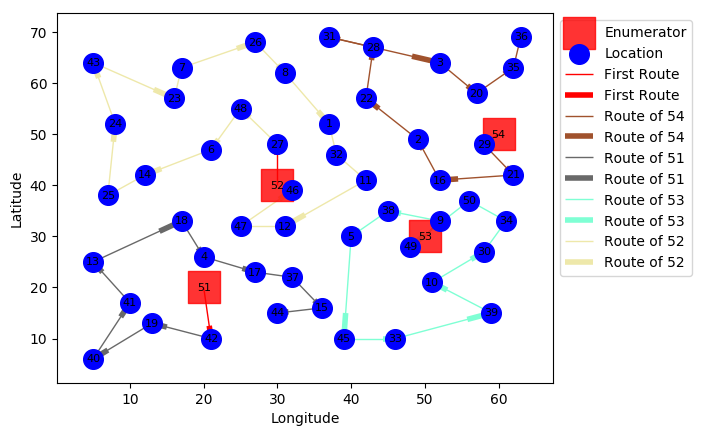
\includegraphics[width=\textwidth]{Resources/Images/cordeau_p01/cordeau_p01_notw_coes}
		\caption{MDVRP berbasis CoEAs}
		\label{fig:cordeau_p01_notw_coes}
	\end{subfigure}
	%
	\begin{subfigure}[t]{\textwidth}
		\centering
		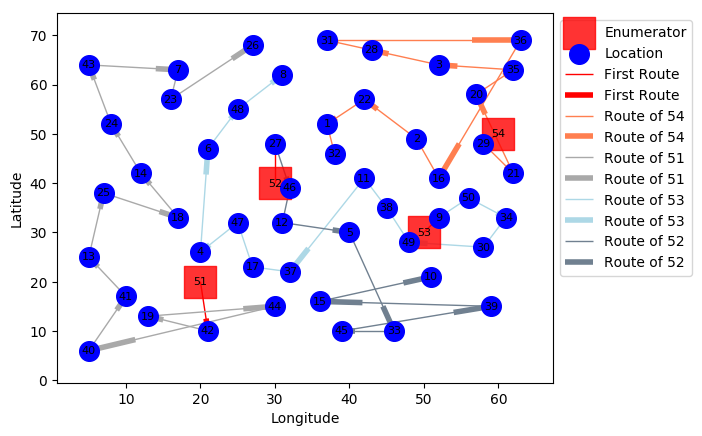
\includegraphics[width=\textwidth]{Resources/Images/cordeau_p01/cordeau_p01_notw_pubsub_coes}
		\caption{MDVRP berbasis CoEAs dengan Publish/Subscribe}
		\label{fig:cordeau_p01_notw_pubsub_coes}
	\end{subfigure}
	\caption{Perbandingan Rute Hasil Pengujian Tanpa \textit{Service Time} Pada Instance Cordeau P01}
	\label{fig:cordeau_p01_notw}
\end{figure}


\begin{figure}[H]
	\centering
	\begin{subfigure}[t]{\textwidth}
		\centering
		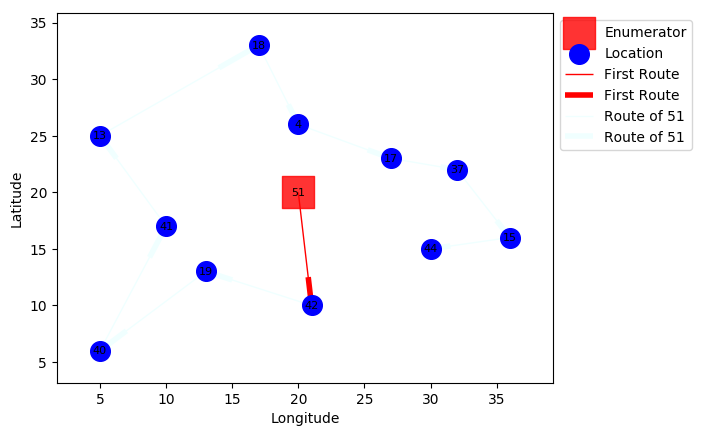
\includegraphics[width=\textwidth]{Resources/Images/cordeau_p01/cordeau_p01_notw_51_coes}
		\caption{MDVRP berbasis CoEAs}
		\label{fig:cordeau_p01_notw_51_coes}
	\end{subfigure}
	%
	\begin{subfigure}[t]{\textwidth}
		\centering
		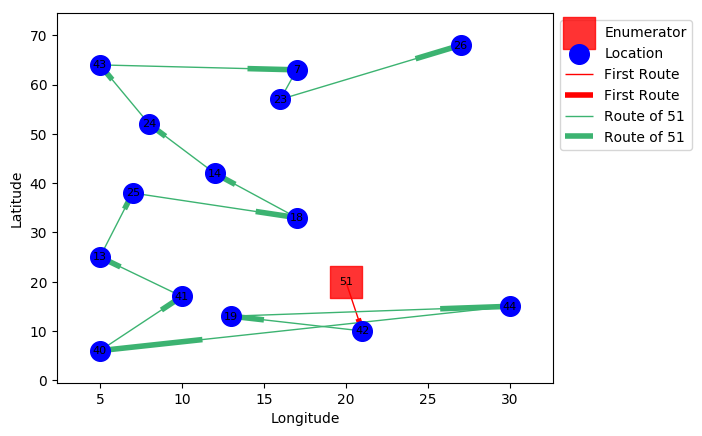
\includegraphics[width=\textwidth]{Resources/Images/cordeau_p01/cordeau_p01_notw_51_pubsub_coes}
		\caption{MDVRP berbasis CoEAs dengan Publish/Subscribe}
		\label{fig:cordeau_p01_notw_51_pubsub_coes}
	\end{subfigure}
	\caption{Perbandingan Rute Hasil Pengujian Tanpa \textit{Service Time} Pada Instance Cordeau P01 Dari Pencacah 51}
	\label{fig:cordeau_p01_notw_51}
\end{figure}


\begin{figure}[H]
	\centering
	\begin{subfigure}[t]{\textwidth}
		\centering
		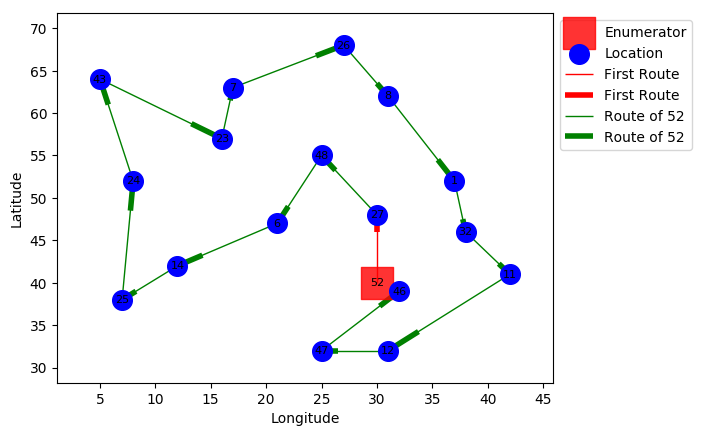
\includegraphics[width=\textwidth]{Resources/Images/cordeau_p01/cordeau_p01_notw_52_coes}
		\caption{MDVRP berbasis CoEAs}
		\label{fig:cordeau_p01_notw_52_coes}
	\end{subfigure}
	%
	\begin{subfigure}[t]{\textwidth}
		\centering
		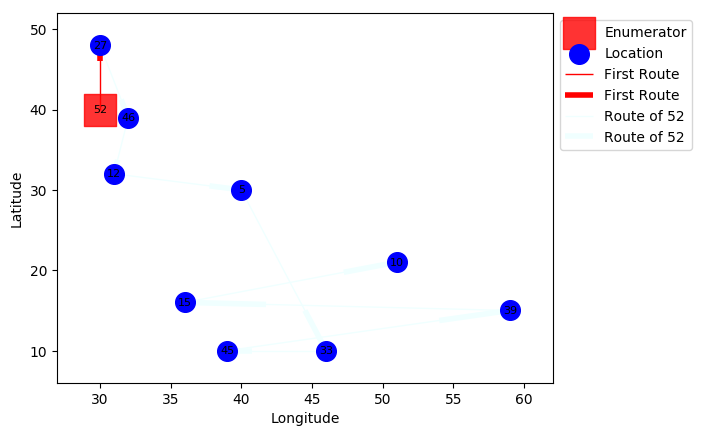
\includegraphics[width=\textwidth]{Resources/Images/cordeau_p01/cordeau_p01_notw_52_pubsub_coes}
		\caption{MDVRP berbasis CoEAs dengan Publish/Subscribe}
		\label{fig:cordeau_p01_notw_52_pubsub_coes}
	\end{subfigure}
	\caption{Perbandingan Rute Hasil Pengujian Tanpa \textit{Service Time} Pada Instance Cordeau P01 Dari Pencacah 52}
	\label{fig:cordeau_p01_notw_52}
\end{figure}


\begin{figure}[H]
	\centering
	\begin{subfigure}[t]{\textwidth}
		\centering
		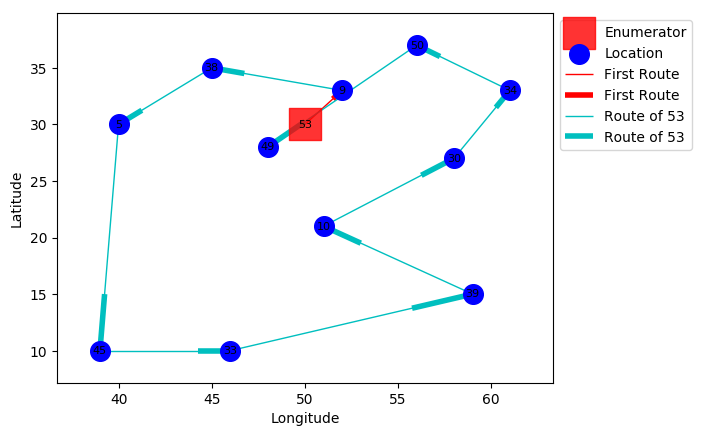
\includegraphics[width=\textwidth]{Resources/Images/cordeau_p01/cordeau_p01_notw_53_coes}
		\caption{MDVRP berbasis CoEAs}
		\label{fig:cordeau_p01_notw_53_coes}
	\end{subfigure}
	%
	\begin{subfigure}[t]{\textwidth}
		\centering
		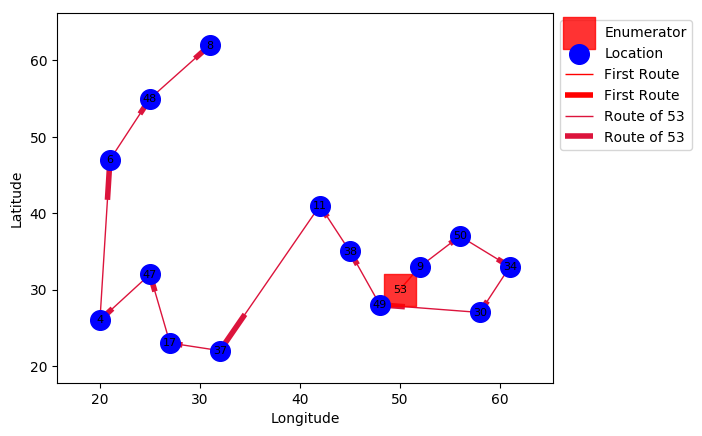
\includegraphics[width=\textwidth]{Resources/Images/cordeau_p01/cordeau_p01_notw_53_pubsub_coes}
		\caption{MDVRP berbasis CoEAs dengan Publish/Subscribe}
		\label{fig:cordeau_p01_notw_53_pubsub_coes}
	\end{subfigure}
	\caption{Perbandingan Rute Hasil Pengujian Tanpa \textit{Service Time} Pada Instance Cordeau P01 Dari Pencacah 53}
	\label{fig:cordeau_p01_notw_53}
\end{figure}


\begin{figure}[H]
	\centering
	\begin{subfigure}[t]{\textwidth}
		\centering
		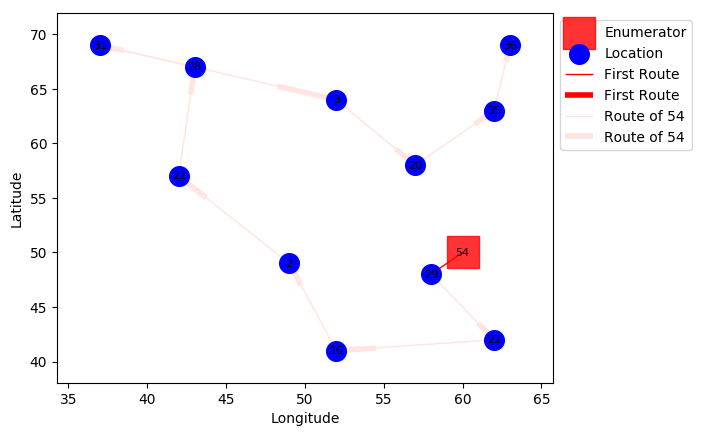
\includegraphics[width=\textwidth]{Resources/Images/cordeau_p01/cordeau_p01_notw_54_coes}
		\caption{MDVRP berbasis CoEAs}
		\label{fig:cordeau_p01_notw_54_coes}
	\end{subfigure}
	%
	\begin{subfigure}[t]{\textwidth}
		\centering
		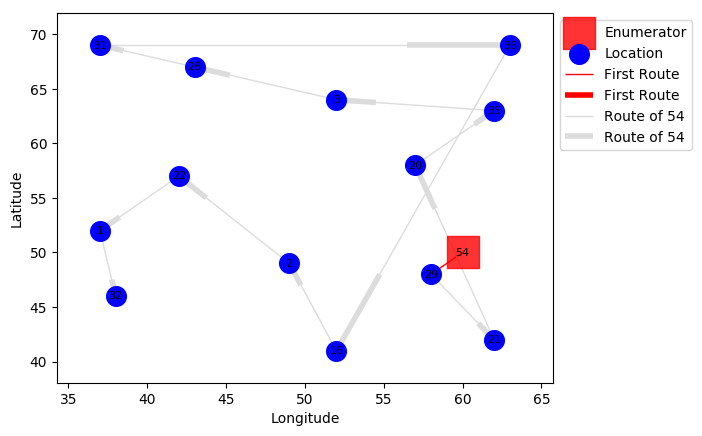
\includegraphics[width=\textwidth]{Resources/Images/cordeau_p01/cordeau_p01_notw_54_pubsub_coes}
		\caption{MDVRP berbasis CoEAs dengan Publish/Subscribe}
		\label{fig:cordeau_p01_notw_54_pubsub_coes}
	\end{subfigure}
	\caption{Perbandingan Rute Hasil Pengujian Tanpa \textit{Service Time} Pada Instance Cordeau P01 Dari Pencacah 54}
	\label{fig:cordeau_p01_notw_54}
\end{figure}


\begin{figure}[H]
	\centering
	\begin{subfigure}[t]{\textwidth}
		\centering
		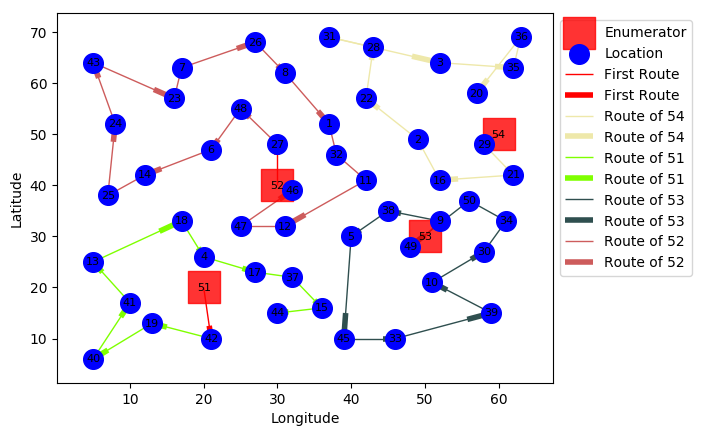
\includegraphics[width=\textwidth]{Resources/Images/cordeau_p02/cordeau_p02_notw_coes}
		\caption{MDVRP berbasis CoEAs}
		\label{fig:cordeau_p02_notw_coes}
	\end{subfigure}
	%
	\begin{subfigure}[t]{\textwidth}
		\centering
		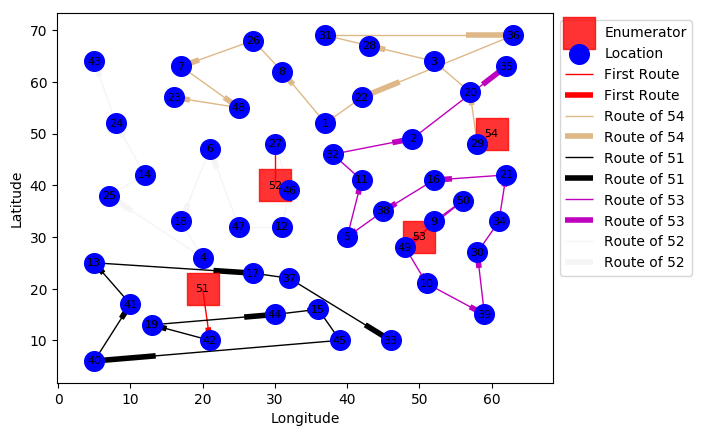
\includegraphics[width=\textwidth]{Resources/Images/cordeau_p02/cordeau_p02_notw_pubsub_coes}
		\caption{MDVRP berbasis CoEAs dengan Publish/Subscribe}
		\label{fig:cordeau_p02_notw_pubsub_coes}
	\end{subfigure}
	\caption{Perbandingan Rute Hasil Pengujian Tanpa \textit{Service Time} Pada Instance Cordeau p02}
	\label{fig:cordeau_p02_notw}
\end{figure}


\begin{figure}[H]
	\centering
	\begin{subfigure}[t]{\textwidth}
		\centering
		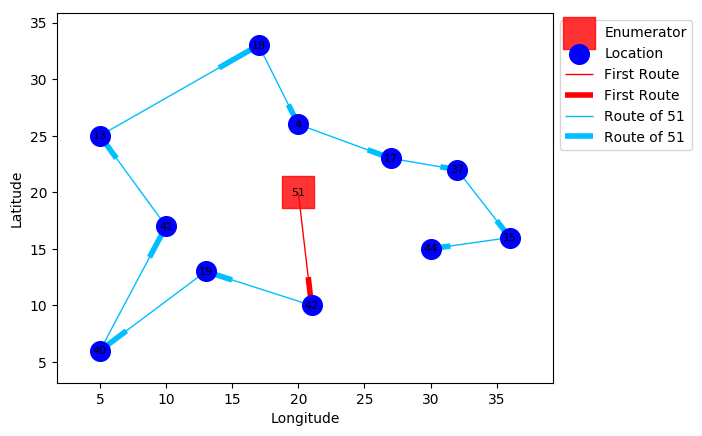
\includegraphics[width=\textwidth]{Resources/Images/cordeau_p02/cordeau_p02_notw_51_coes}
		\caption{MDVRP berbasis CoEAs}
		\label{fig:cordeau_p02_notw_51_coes}
	\end{subfigure}
	%
	\begin{subfigure}[t]{\textwidth}
		\centering
		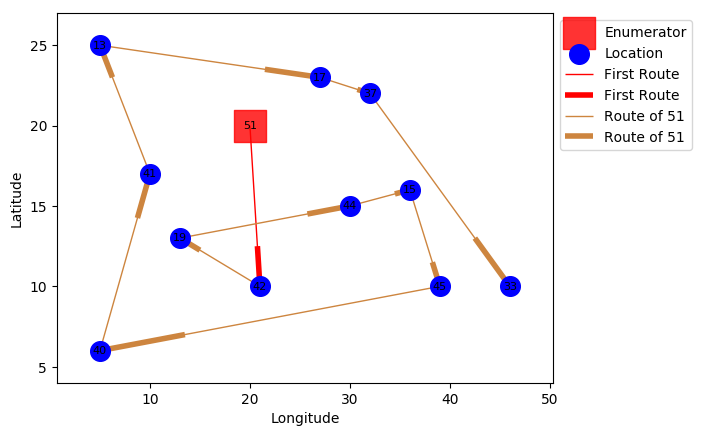
\includegraphics[width=\textwidth]{Resources/Images/cordeau_p02/cordeau_p02_notw_51_pubsub_coes}
		\caption{MDVRP berbasis CoEAs dengan Publish/Subscribe}
		\label{fig:cordeau_p02_notw_51_pubsub_coes}
	\end{subfigure}
	\caption{Perbandingan Rute Hasil Pengujian Tanpa \textit{Service Time} Pada Instance Cordeau p02 Dari Pencacah 51}
	\label{fig:cordeau_p02_notw_51}
\end{figure}


\begin{figure}[H]
	\centering
	\begin{subfigure}[t]{\textwidth}
		\centering
		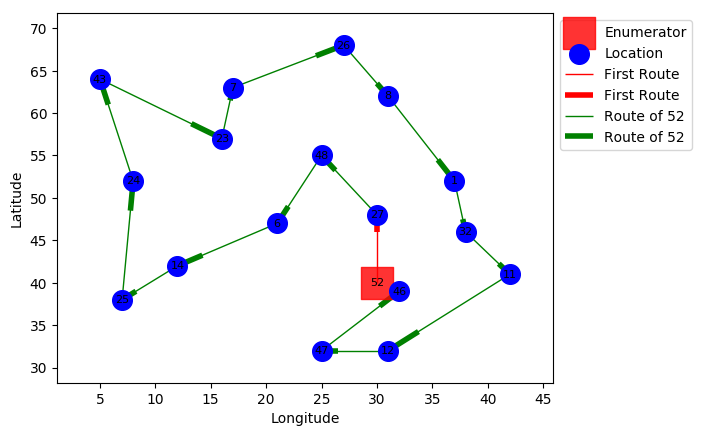
\includegraphics[width=\textwidth]{Resources/Images/cordeau_p02/cordeau_p02_notw_52_coes}
		\caption{MDVRP berbasis CoEAs}
		\label{fig:cordeau_p02_notw_52_coes}
	\end{subfigure}
	%
	\begin{subfigure}[t]{\textwidth}
		\centering
		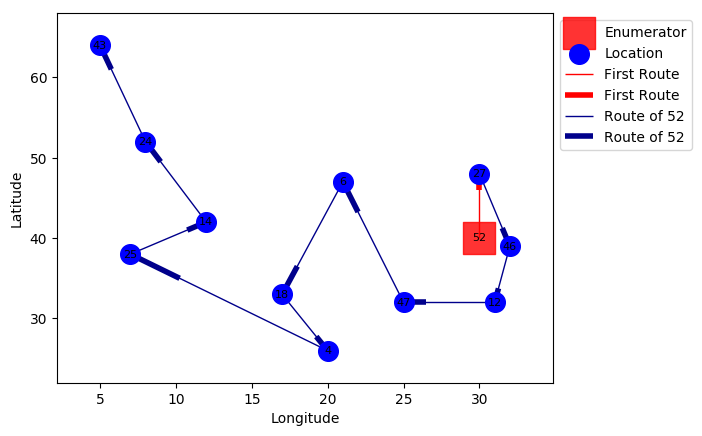
\includegraphics[width=\textwidth]{Resources/Images/cordeau_p02/cordeau_p02_notw_52_pubsub_coes}
		\caption{MDVRP berbasis CoEAs dengan Publish/Subscribe}
		\label{fig:cordeau_p02_notw_52_pubsub_coes}
	\end{subfigure}
	\caption{Perbandingan Rute Hasil Pengujian Tanpa \textit{Service Time} Pada Instance Cordeau p02 Dari Pencacah 52}
	\label{fig:cordeau_p02_notw_52}
\end{figure}


\begin{figure}[H]
	\centering
	\begin{subfigure}[t]{\textwidth}
		\centering
		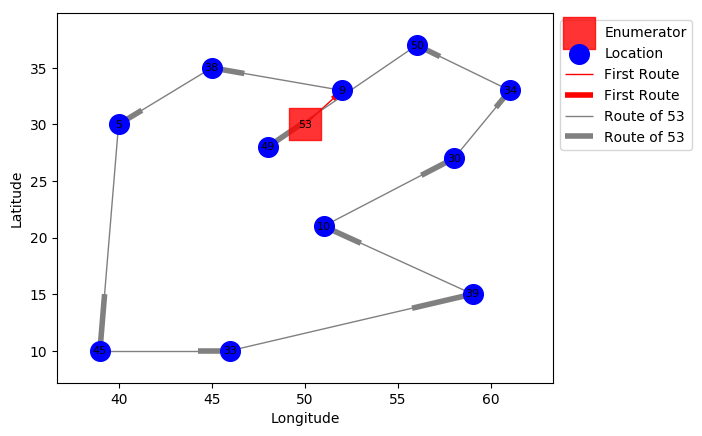
\includegraphics[width=\textwidth]{Resources/Images/cordeau_p02/cordeau_p02_notw_53_coes}
		\caption{MDVRP berbasis CoEAs}
		\label{fig:cordeau_p02_notw_53_coes}
	\end{subfigure}
	%
	\begin{subfigure}[t]{\textwidth}
		\centering
		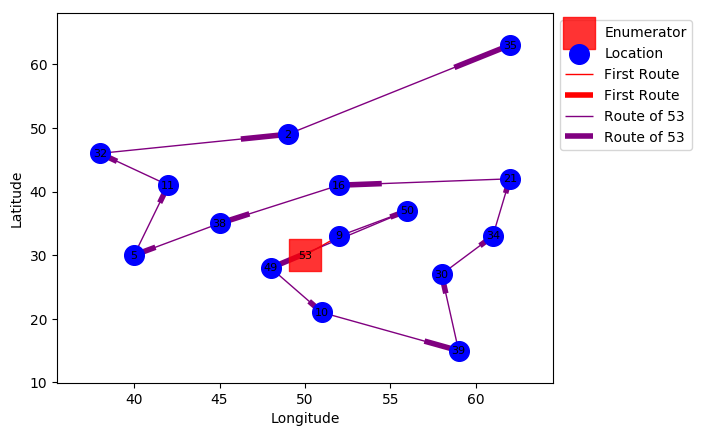
\includegraphics[width=\textwidth]{Resources/Images/cordeau_p02/cordeau_p02_notw_53_pubsub_coes}
		\caption{MDVRP berbasis CoEAs dengan Publish/Subscribe}
		\label{fig:cordeau_p02_notw_53_pubsub_coes}
	\end{subfigure}
	\caption{Perbandingan Rute Hasil Pengujian Tanpa \textit{Service Time} Pada Instance Cordeau p02 Dari Pencacah 53}
	\label{fig:cordeau_p02_notw_53}
\end{figure}


\begin{figure}[H]
	\centering
	\begin{subfigure}[t]{\textwidth}
		\centering
		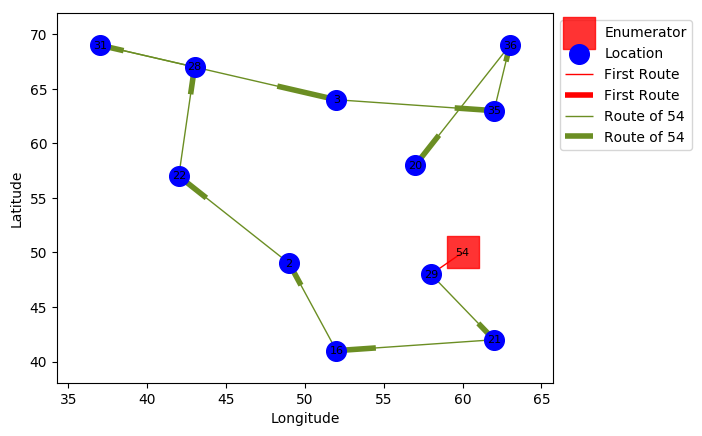
\includegraphics[width=\textwidth]{Resources/Images/cordeau_p02/cordeau_p02_notw_54_coes}
		\caption{MDVRP berbasis CoEAs}
		\label{fig:cordeau_p02_notw_54_coes}
	\end{subfigure}
	%
	\begin{subfigure}[t]{\textwidth}
		\centering
		\includegraphics[width=\textwidth]{Resources/Images/cordeau_p02/cordeau_p02_notw_54_pubsub_coes}
		\caption{MDVRP berbasis CoEAs dengan Publish/Subscribe}
		\label{fig:cordeau_p02_notw_54_pubsub_coes}
	\end{subfigure}
	\caption{Perbandingan Rute Hasil Pengujian Tanpa \textit{Service Time} Pada Instance Cordeau p02 Dari Pencacah 54}
	\label{fig:cordeau_p02_notw_54}
\end{figure}


\begin{figure}[H]
	\centering
	\begin{subfigure}[t]{\textwidth}
		\centering
		\includegraphics[width=\textwidth]{Resources/Images/cordeau_p03/cordeau_p03_notw_coes}
		\caption{MDVRP berbasis CoEAs}
		\label{fig:cordeau_p03_notw_coes}
	\end{subfigure}
	%
	\begin{subfigure}[t]{\textwidth}
		\centering
		\includegraphics[width=\textwidth]{Resources/Images/cordeau_p03/cordeau_p03_notw_pubsub_coes}
		\caption{MDVRP berbasis CoEAs dengan Publish/Subscribe}
		\label{fig:cordeau_p03_notw_pubsub_coes}
	\end{subfigure}
	\caption{Perbandingan Rute Hasil Pengujian Tanpa \textit{Service Time} Pada Instance Cordeau p03}
	\label{fig:cordeau_p03_notw}
\end{figure}


\begin{figure}[H]
	\centering
	\begin{subfigure}[t]{\textwidth}
		\centering
		\includegraphics[width=\textwidth]{Resources/Images/cordeau_p03/cordeau_p03_notw_76_coes}
		\caption{MDVRP berbasis CoEAs}
		\label{fig:cordeau_p03_notw_76_coes}
	\end{subfigure}
	%
	\begin{subfigure}[t]{\textwidth}
		\centering
		\includegraphics[width=\textwidth]{Resources/Images/cordeau_p03/cordeau_p03_notw_76_pubsub_coes}
		\caption{MDVRP berbasis CoEAs dengan Publish/Subscribe}
		\label{fig:cordeau_p03_notw_76_pubsub_coes}
	\end{subfigure}
	\caption{Perbandingan Rute Hasil Pengujian Tanpa \textit{Service Time} Pada Instance Cordeau p03 Dari Pencacah 76}
	\label{fig:cordeau_p03_notw_76}
\end{figure}


\begin{figure}[H]
	\centering
	\begin{subfigure}[t]{\textwidth}
		\centering
		\includegraphics[width=\textwidth]{Resources/Images/cordeau_p03/cordeau_p03_notw_77_coes}
		\caption{MDVRP berbasis CoEAs}
		\label{fig:cordeau_p03_notw_77_coes}
	\end{subfigure}
	%
	\begin{subfigure}[t]{\textwidth}
		\centering
		\includegraphics[width=\textwidth]{Resources/Images/cordeau_p03/cordeau_p03_notw_77_pubsub_coes}
		\caption{MDVRP berbasis CoEAs dengan Publish/Subscribe}
		\label{fig:cordeau_p03_notw_77_pubsub_coes}
	\end{subfigure}
	\caption{Perbandingan Rute Hasil Pengujian Tanpa \textit{Service Time} Pada Instance Cordeau p03 Dari Pencacah 77}
	\label{fig:cordeau_p03_notw_77}
\end{figure}


\begin{figure}[H]
	\centering
	\begin{subfigure}[t]{\textwidth}
		\centering
		\includegraphics[width=\textwidth]{Resources/Images/cordeau_p03/cordeau_p03_notw_78_coes}
		\caption{MDVRP berbasis CoEAs}
		\label{fig:cordeau_p03_notw_78_coes}
	\end{subfigure}
	%
	\begin{subfigure}[t]{\textwidth}
		\centering
		\includegraphics[width=\textwidth]{Resources/Images/cordeau_p03/cordeau_p03_notw_78_pubsub_coes}
		\caption{MDVRP berbasis CoEAs dengan Publish/Subscribe}
		\label{fig:cordeau_p03_notw_78_pubsub_coes}
	\end{subfigure}
	\caption{Perbandingan Rute Hasil Pengujian Tanpa \textit{Service Time} Pada Instance Cordeau p03 Dari Pencacah 78}
	\label{fig:cordeau_p03_notw_78}
\end{figure}


\begin{figure}[H]
	\centering
	\begin{subfigure}[t]{\textwidth}
		\centering
		\includegraphics[width=\textwidth]{Resources/Images/cordeau_p03/cordeau_p03_notw_79_coes}
		\caption{MDVRP berbasis CoEAs}
		\label{fig:cordeau_p03_notw_79_coes}
	\end{subfigure}
	%
	\begin{subfigure}[t]{\textwidth}
		\centering
		\includegraphics[width=\textwidth]{Resources/Images/cordeau_p03/cordeau_p03_notw_79_pubsub_coes}
		\caption{MDVRP berbasis CoEAs dengan Publish/Subscribe}
		\label{fig:cordeau_p03_notw_79_pubsub_coes}
	\end{subfigure}
	\caption{Perbandingan Rute Hasil Pengujian Tanpa \textit{Service Time} Pada Instance Cordeau p03 Dari Pencacah 79}
	\label{fig:cordeau_p03_notw_79}
\end{figure}


\begin{figure}[H]
	\centering
	\begin{subfigure}[t]{\textwidth}
		\centering
		\includegraphics[width=\textwidth]{Resources/Images/cordeau_p03/cordeau_p03_notw_80_coes}
		\caption{MDVRP berbasis CoEAs}
		\label{fig:cordeau_p03_notw_80_coes}
	\end{subfigure}
	%
	\begin{subfigure}[t]{\textwidth}
		\centering
		\includegraphics[width=\textwidth]{Resources/Images/cordeau_p03/cordeau_p03_notw_80_pubsub_coes}
		\caption{MDVRP berbasis CoEAs dengan Publish/Subscribe}
		\label{fig:cordeau_p03_notw_80_pubsub_coes}
	\end{subfigure}
	\caption{Perbandingan Rute Hasil Pengujian Tanpa \textit{Service Time} Pada Instance Cordeau p03 Dari Pencacah 80}
	\label{fig:cordeau_p03_notw_80}
\end{figure}


\begin{figure}[H]
	\centering
	\begin{subfigure}[t]{\textwidth}
		\centering
		\includegraphics[width=\textwidth]{Resources/Images/cordeau_p04/cordeau_p04_notw_coes}
		\caption{MDVRP berbasis CoEAs}
		\label{fig:cordeau_p04_notw_coes}
	\end{subfigure}
	%
	\begin{subfigure}[t]{\textwidth}
		\centering
		\includegraphics[width=\textwidth]{Resources/Images/cordeau_p04/cordeau_p04_notw_pubsub_coes}
		\caption{MDVRP berbasis CoEAs dengan Publish/Subscribe}
		\label{fig:cordeau_p04_notw_pubsub_coes}
	\end{subfigure}
	\caption{Perbandingan Rute Hasil Pengujian Tanpa \textit{Service Time} Pada Instance Cordeau p04}
	\label{fig:cordeau_p04_notw}
\end{figure}


\begin{figure}[H]
	\centering
	\begin{subfigure}[t]{\textwidth}
		\centering
		\includegraphics[width=\textwidth]{Resources/Images/cordeau_p04/cordeau_p04_notw_101_coes}
		\caption{MDVRP berbasis CoEAs}
		\label{fig:cordeau_p04_notw_101_coes}
	\end{subfigure}
	%
	\begin{subfigure}[t]{\textwidth}
		\centering
		\includegraphics[width=\textwidth]{Resources/Images/cordeau_p04/cordeau_p04_notw_101_pubsub_coes}
		\caption{MDVRP berbasis CoEAs dengan Publish/Subscribe}
		\label{fig:cordeau_p04_notw_101_pubsub_coes}
	\end{subfigure}
	\caption{Perbandingan Rute Hasil Pengujian Tanpa \textit{Service Time} Pada Instance Cordeau p04 Dari Pencacah 101}
	\label{fig:cordeau_p04_notw_101}
\end{figure}


\begin{figure}[H]
	\centering
	\begin{subfigure}[t]{\textwidth}
		\centering
		\includegraphics[width=\textwidth]{Resources/Images/cordeau_p04/cordeau_p04_notw_102_coes}
		\caption{MDVRP berbasis CoEAs}
		\label{fig:cordeau_p04_notw_102_coes}
	\end{subfigure}
	%
	\begin{subfigure}[t]{\textwidth}
		\centering
		\includegraphics[width=\textwidth]{Resources/Images/cordeau_p04/cordeau_p04_notw_102_pubsub_coes}
		\caption{MDVRP berbasis CoEAs dengan Publish/Subscribe}
		\label{fig:cordeau_p04_notw_102_pubsub_coes}
	\end{subfigure}
	\caption{Perbandingan Rute Hasil Pengujian Tanpa \textit{Service Time} Pada Instance Cordeau p04 Dari Pencacah 102}
	\label{fig:cordeau_p04_notw_102}
\end{figure}


\begin{figure}[H]
	\centering
	\begin{subfigure}[t]{\textwidth}
		\centering
		\includegraphics[width=\textwidth]{Resources/Images/cordeau_p05/cordeau_p05_notw_coes}
		\caption{MDVRP berbasis CoEAs}
		\label{fig:cordeau_p05_notw_coes}
	\end{subfigure}
	%
	\begin{subfigure}[t]{\textwidth}
		\centering
		\includegraphics[width=\textwidth]{Resources/Images/cordeau_p05/cordeau_p05_notw_pubsub_coes}
		\caption{MDVRP berbasis CoEAs dengan Publish/Subscribe}
		\label{fig:cordeau_p05_notw_pubsub_coes}
	\end{subfigure}
	\caption{Perbandingan Rute Hasil Pengujian Tanpa \textit{Service Time} Pada Instance Cordeau p05}
	\label{fig:cordeau_p05_notw}
\end{figure}


\begin{figure}[H]
	\centering
	\begin{subfigure}[t]{\textwidth}
		\centering
		\includegraphics[width=\textwidth]{Resources/Images/cordeau_p05/cordeau_p05_notw_101_coes}
		\caption{MDVRP berbasis CoEAs}
		\label{fig:cordeau_p05_notw_101_coes}
	\end{subfigure}
	%
	\begin{subfigure}[t]{\textwidth}
		\centering
		\includegraphics[width=\textwidth]{Resources/Images/cordeau_p05/cordeau_p05_notw_101_pubsub_coes}
		\caption{MDVRP berbasis CoEAs dengan Publish/Subscribe}
		\label{fig:cordeau_p05_notw_101_pubsub_coes}
	\end{subfigure}
	\caption{Perbandingan Rute Hasil Pengujian Tanpa \textit{Service Time} Pada Instance Cordeau p05 Dari Pencacah 101}
	\label{fig:cordeau_p05_notw_101}
\end{figure}


\begin{figure}[H]
	\centering
	\begin{subfigure}[t]{\textwidth}
		\centering
		\includegraphics[width=\textwidth]{Resources/Images/cordeau_p05/cordeau_p05_notw_102_coes}
		\caption{MDVRP berbasis CoEAs}
		\label{fig:cordeau_p05_notw_102_coes}
	\end{subfigure}
	%
	\begin{subfigure}[t]{\textwidth}
		\centering
		\includegraphics[width=\textwidth]{Resources/Images/cordeau_p05/cordeau_p05_notw_102_pubsub_coes}
		\caption{MDVRP berbasis CoEAs dengan Publish/Subscribe}
		\label{fig:cordeau_p05_notw_102_pubsub_coes}
	\end{subfigure}
	\caption{Perbandingan Rute Hasil Pengujian Tanpa \textit{Service Time} Pada Instance Cordeau p05 Dari Pencacah 102}
	\label{fig:cordeau_p05_notw_102}
\end{figure}


\begin{figure}[H]
	\centering
	\begin{subfigure}[t]{\textwidth}
		\centering
		\includegraphics[width=\textwidth]{Resources/Images/cordeau_p06/cordeau_p06_notw_coes}
		\caption{MDVRP berbasis CoEAs}
		\label{fig:cordeau_p06_notw_coes}
	\end{subfigure}
	%
	\begin{subfigure}[t]{\textwidth}
		\centering
		\includegraphics[width=\textwidth]{Resources/Images/cordeau_p06/cordeau_p06_notw_pubsub_coes}
		\caption{MDVRP berbasis CoEAs dengan Publish/Subscribe}
		\label{fig:cordeau_p06_notw_pubsub_coes}
	\end{subfigure}
	\caption{Perbandingan Rute Hasil Pengujian Tanpa \textit{Service Time} Pada Instance Cordeau p06}
	\label{fig:cordeau_p06_notw}
\end{figure}


\begin{figure}[H]
	\centering
	\begin{subfigure}[t]{\textwidth}
		\centering
		\includegraphics[width=\textwidth]{Resources/Images/cordeau_p06/cordeau_p06_notw_101_coes}
		\caption{MDVRP berbasis CoEAs}
		\label{fig:cordeau_p06_notw_101_coes}
	\end{subfigure}
	%
	\begin{subfigure}[t]{\textwidth}
		\centering
		\includegraphics[width=\textwidth]{Resources/Images/cordeau_p06/cordeau_p06_notw_101_pubsub_coes}
		\caption{MDVRP berbasis CoEAs dengan Publish/Subscribe}
		\label{fig:cordeau_p06_notw_101_pubsub_coes}
	\end{subfigure}
	\caption{Perbandingan Rute Hasil Pengujian Tanpa \textit{Service Time} Pada Instance Cordeau p06 Dari Pencacah 101}
	\label{fig:cordeau_p06_notw_101}
\end{figure}


\begin{figure}[H]
	\centering
	\begin{subfigure}[t]{\textwidth}
		\centering
		\includegraphics[width=\textwidth]{Resources/Images/cordeau_p06/cordeau_p06_notw_102_coes}
		\caption{MDVRP berbasis CoEAs}
		\label{fig:cordeau_p06_notw_102_coes}
	\end{subfigure}
	%
	\begin{subfigure}[t]{\textwidth}
		\centering
		\includegraphics[width=\textwidth]{Resources/Images/cordeau_p06/cordeau_p06_notw_102_pubsub_coes}
		\caption{MDVRP berbasis CoEAs dengan Publish/Subscribe}
		\label{fig:cordeau_p06_notw_102_pubsub_coes}
	\end{subfigure}
	\caption{Perbandingan Rute Hasil Pengujian Tanpa \textit{Service Time} Pada Instance Cordeau p06 Dari Pencacah 102}
	\label{fig:cordeau_p06_notw_102}
\end{figure}


\begin{figure}[H]
	\centering
	\begin{subfigure}[t]{\textwidth}
		\centering
		\includegraphics[width=\textwidth]{Resources/Images/cordeau_p06/cordeau_p06_notw_103_coes}
		\caption{MDVRP berbasis CoEAs}
		\label{fig:cordeau_p06_notw_103_coes}
	\end{subfigure}
	%
	\begin{subfigure}[t]{\textwidth}
		\centering
		\includegraphics[width=\textwidth]{Resources/Images/cordeau_p06/cordeau_p06_notw_103_pubsub_coes}
		\caption{MDVRP berbasis CoEAs dengan Publish/Subscribe}
		\label{fig:cordeau_p06_notw_103_pubsub_coes}
	\end{subfigure}
	\caption{Perbandingan Rute Hasil Pengujian Tanpa \textit{Service Time} Pada Instance Cordeau p06 Dari Pencacah 103}
	\label{fig:cordeau_p06_notw_103}
\end{figure}


\begin{figure}[H]
	\centering
	\begin{subfigure}[t]{\textwidth}
		\centering
		\includegraphics[width=\textwidth]{Resources/Images/cordeau_p07/cordeau_p07_notw_coes}
		\caption{MDVRP berbasis CoEAs}
		\label{fig:cordeau_p07_notw_coes}
	\end{subfigure}
	%
	\begin{subfigure}[t]{\textwidth}
		\centering
		\includegraphics[width=\textwidth]{Resources/Images/cordeau_p07/cordeau_p07_notw_pubsub_coes}
		\caption{MDVRP berbasis CoEAs dengan Publish/Subscribe}
		\label{fig:cordeau_p07_notw_pubsub_coes}
	\end{subfigure}
	\caption{Perbandingan Rute Hasil Pengujian Tanpa \textit{Service Time} Pada Instance Cordeau p07}
	\label{fig:cordeau_p07_notw}
\end{figure}


\begin{figure}[H]
	\centering
	\begin{subfigure}[t]{\textwidth}
		\centering
		\includegraphics[width=\textwidth]{Resources/Images/cordeau_p07/cordeau_p07_notw_101_coes}
		\caption{MDVRP berbasis CoEAs}
		\label{fig:cordeau_p07_notw_101_coes}
	\end{subfigure}
	%
	\begin{subfigure}[t]{\textwidth}
		\centering
		\includegraphics[width=\textwidth]{Resources/Images/cordeau_p07/cordeau_p07_notw_101_pubsub_coes}
		\caption{MDVRP berbasis CoEAs dengan Publish/Subscribe}
		\label{fig:cordeau_p07_notw_101_pubsub_coes}
	\end{subfigure}
	\caption{Perbandingan Rute Hasil Pengujian Tanpa \textit{Service Time} Pada Instance Cordeau p07 Dari Pencacah 101}
	\label{fig:cordeau_p07_notw_101}
\end{figure}


\begin{figure}[H]
	\centering
	\begin{subfigure}[t]{\textwidth}
		\centering
		\includegraphics[width=\textwidth]{Resources/Images/cordeau_p07/cordeau_p07_notw_102_coes}
		\caption{MDVRP berbasis CoEAs}
		\label{fig:cordeau_p07_notw_102_coes}
	\end{subfigure}
	%
	\begin{subfigure}[t]{\textwidth}
		\centering
		\includegraphics[width=\textwidth]{Resources/Images/cordeau_p07/cordeau_p07_notw_102_pubsub_coes}
		\caption{MDVRP berbasis CoEAs dengan Publish/Subscribe}
		\label{fig:cordeau_p07_notw_102_pubsub_coes}
	\end{subfigure}
	\caption{Perbandingan Rute Hasil Pengujian Tanpa \textit{Service Time} Pada Instance Cordeau p07 Dari Pencacah 102}
	\label{fig:cordeau_p07_notw_102}
\end{figure}


\begin{figure}[H]
	\centering
	\begin{subfigure}[t]{\textwidth}
		\centering
		\includegraphics[width=\textwidth]{Resources/Images/cordeau_p07/cordeau_p07_notw_103_coes}
		\caption{MDVRP berbasis CoEAs}
		\label{fig:cordeau_p07_notw_103_coes}
	\end{subfigure}
	%
	\begin{subfigure}[t]{\textwidth}
		\centering
		\includegraphics[width=\textwidth]{Resources/Images/cordeau_p07/cordeau_p07_notw_103_pubsub_coes}
		\caption{MDVRP berbasis CoEAs dengan Publish/Subscribe}
		\label{fig:cordeau_p07_notw_103_pubsub_coes}
	\end{subfigure}
	\caption{Perbandingan Rute Hasil Pengujian Tanpa \textit{Service Time} Pada Instance Cordeau p07 Dari Pencacah 103}
	\label{fig:cordeau_p07_notw_103}
\end{figure}


\begin{figure}[H]
	\centering
	\begin{subfigure}[t]{\textwidth}
		\centering
		\includegraphics[width=\textwidth]{Resources/Images/cordeau_p07/cordeau_p07_notw_104_coes}
		\caption{MDVRP berbasis CoEAs}
		\label{fig:cordeau_p07_notw_104_coes}
	\end{subfigure}
	%
	\begin{subfigure}[t]{\textwidth}
		\centering
		\includegraphics[width=\textwidth]{Resources/Images/cordeau_p07/cordeau_p07_notw_104_pubsub_coes}
		\caption{MDVRP berbasis CoEAs dengan Publish/Subscribe}
		\label{fig:cordeau_p07_notw_104_pubsub_coes}
	\end{subfigure}
	\caption{Perbandingan Rute Hasil Pengujian Tanpa \textit{Service Time} Pada Instance Cordeau p07 Dari Pencacah 104}
	\label{fig:cordeau_p07_notw_104}
\end{figure}


\begin{figure}[H]
	\centering
	\begin{subfigure}[t]{\textwidth}
		\centering
		\includegraphics[width=\textwidth]{Resources/Images/cordeau_p08/cordeau_p08_notw_coes}
		\caption{MDVRP berbasis CoEAs}
		\label{fig:cordeau_p08_notw_coes}
	\end{subfigure}
	%
	\begin{subfigure}[t]{\textwidth}
		\centering
		\includegraphics[width=\textwidth]{Resources/Images/cordeau_p08/cordeau_p08_notw_pubsub_coes}
		\caption{MDVRP berbasis CoEAs dengan Publish/Subscribe}
		\label{fig:cordeau_p08_notw_pubsub_coes}
	\end{subfigure}
	\caption{Perbandingan Rute Hasil Pengujian Tanpa \textit{Service Time} Pada Instance Cordeau p08}
	\label{fig:cordeau_p08_notw}
\end{figure}


\begin{figure}[H]
	\centering
	\begin{subfigure}[t]{\textwidth}
		\centering
		\includegraphics[width=\textwidth]{Resources/Images/cordeau_p08/cordeau_p08_notw_250_coes}
		\caption{MDVRP berbasis CoEAs}
		\label{fig:cordeau_p08_notw_250_coes}
	\end{subfigure}
	%
	\begin{subfigure}[t]{\textwidth}
		\centering
		\includegraphics[width=\textwidth]{Resources/Images/cordeau_p08/cordeau_p08_notw_250_pubsub_coes}
		\caption{MDVRP berbasis CoEAs dengan Publish/Subscribe}
		\label{fig:cordeau_p08_notw_250_pubsub_coes}
	\end{subfigure}
	\caption{Perbandingan Rute Hasil Pengujian Tanpa \textit{Service Time} Pada Instance Cordeau p08 Dari Pencacah 250}
	\label{fig:cordeau_p08_notw_250}
\end{figure}


\begin{figure}[H]
	\centering
	\begin{subfigure}[t]{\textwidth}
		\centering
		\includegraphics[width=\textwidth]{Resources/Images/cordeau_p08/cordeau_p08_notw_251_coes}
		\caption{MDVRP berbasis CoEAs}
		\label{fig:cordeau_p08_notw_251_coes}
	\end{subfigure}
	%
	\begin{subfigure}[t]{\textwidth}
		\centering
		\includegraphics[width=\textwidth]{Resources/Images/cordeau_p08/cordeau_p08_notw_251_pubsub_coes}
		\caption{MDVRP berbasis CoEAs dengan Publish/Subscribe}
		\label{fig:cordeau_p08_notw_251_pubsub_coes}
	\end{subfigure}
	\caption{Perbandingan Rute Hasil Pengujian Tanpa \textit{Service Time} Pada Instance Cordeau p08 Dari Pencacah 251}
	\label{fig:cordeau_p08_notw_251}
\end{figure}


\begin{figure}[H]
	\centering
	\begin{subfigure}[t]{\textwidth}
		\centering
		\includegraphics[width=\textwidth]{Resources/Images/cordeau_p09/cordeau_p09_notw_coes}
		\caption{MDVRP berbasis CoEAs}
		\label{fig:cordeau_p09_notw_coes}
	\end{subfigure}
	%
	\begin{subfigure}[t]{\textwidth}
		\centering
		\includegraphics[width=\textwidth]{Resources/Images/cordeau_p09/cordeau_p09_notw_pubsub_coes}
		\caption{MDVRP berbasis CoEAs dengan Publish/Subscribe}
		\label{fig:cordeau_p09_notw_pubsub_coes}
	\end{subfigure}
	\caption{Perbandingan Rute Hasil Pengujian Tanpa \textit{Service Time} Pada Instance Cordeau p09}
	\label{fig:cordeau_p09_notw}
\end{figure}


\begin{figure}[H]
	\centering
	\begin{subfigure}[t]{\textwidth}
		\centering
		\includegraphics[width=\textwidth]{Resources/Images/cordeau_p09/cordeau_p09_notw_250_coes}
		\caption{MDVRP berbasis CoEAs}
		\label{fig:cordeau_p09_notw_250_coes}
	\end{subfigure}
	%
	\begin{subfigure}[t]{\textwidth}
		\centering
		\includegraphics[width=\textwidth]{Resources/Images/cordeau_p09/cordeau_p09_notw_250_pubsub_coes}
		\caption{MDVRP berbasis CoEAs dengan Publish/Subscribe}
		\label{fig:cordeau_p09_notw_250_pubsub_coes}
	\end{subfigure}
	\caption{Perbandingan Rute Hasil Pengujian Tanpa \textit{Service Time} Pada Instance Cordeau p09 Dari Pencacah 250}
	\label{fig:cordeau_p09_notw_250}
\end{figure}


\begin{figure}[H]
	\centering
	\begin{subfigure}[t]{\textwidth}
		\centering
		\includegraphics[width=\textwidth]{Resources/Images/cordeau_p09/cordeau_p09_notw_251_coes}
		\caption{MDVRP berbasis CoEAs}
		\label{fig:cordeau_p09_notw_251_coes}
	\end{subfigure}
	%
	\begin{subfigure}[t]{\textwidth}
		\centering
		\includegraphics[width=\textwidth]{Resources/Images/cordeau_p09/cordeau_p09_notw_251_pubsub_coes}
		\caption{MDVRP berbasis CoEAs dengan Publish/Subscribe}
		\label{fig:cordeau_p09_notw_251_pubsub_coes}
	\end{subfigure}
	\caption{Perbandingan Rute Hasil Pengujian Tanpa \textit{Service Time} Pada Instance Cordeau p09 Dari Pencacah 251}
	\label{fig:cordeau_p09_notw_251}
\end{figure}


\begin{figure}[H]
	\centering
	\begin{subfigure}[t]{\textwidth}
		\centering
		\includegraphics[width=\textwidth]{Resources/Images/cordeau_p09/cordeau_p09_notw_252_coes}
		\caption{MDVRP berbasis CoEAs}
		\label{fig:cordeau_p09_notw_252_coes}
	\end{subfigure}
	%
	\begin{subfigure}[t]{\textwidth}
		\centering
		\includegraphics[width=\textwidth]{Resources/Images/cordeau_p09/cordeau_p09_notw_252_pubsub_coes}
		\caption{MDVRP berbasis CoEAs dengan Publish/Subscribe}
		\label{fig:cordeau_p09_notw_252_pubsub_coes}
	\end{subfigure}
	\caption{Perbandingan Rute Hasil Pengujian Tanpa \textit{Service Time} Pada Instance Cordeau p09 Dari Pencacah 252}
	\label{fig:cordeau_p09_notw_252}
\end{figure}


\begin{figure}[H]
	\centering
	\begin{subfigure}[t]{\textwidth}
		\centering
		\includegraphics[width=\textwidth]{Resources/Images/cordeau_p10/cordeau_p10_notw_coes}
		\caption{MDVRP berbasis CoEAs}
		\label{fig:cordeau_p10_notw_coes}
	\end{subfigure}
	%
	\begin{subfigure}[t]{\textwidth}
		\centering
		\includegraphics[width=\textwidth]{Resources/Images/cordeau_p10/cordeau_p10_notw_pubsub_coes}
		\caption{MDVRP berbasis CoEAs dengan Publish/Subscribe}
		\label{fig:cordeau_p10_notw_pubsub_coes}
	\end{subfigure}
	\caption{Perbandingan Rute Hasil Pengujian Tanpa \textit{Service Time} Pada Instance Cordeau p10}
	\label{fig:cordeau_p10_notw}
\end{figure}


\begin{figure}[H]
	\centering
	\begin{subfigure}[t]{\textwidth}
		\centering
		\includegraphics[width=\textwidth]{Resources/Images/cordeau_p10/cordeau_p10_notw_250_coes}
		\caption{MDVRP berbasis CoEAs}
		\label{fig:cordeau_p10_notw_250_coes}
	\end{subfigure}
	%
	\begin{subfigure}[t]{\textwidth}
		\centering
		\includegraphics[width=\textwidth]{Resources/Images/cordeau_p10/cordeau_p10_notw_250_pubsub_coes}
		\caption{MDVRP berbasis CoEAs dengan Publish/Subscribe}
		\label{fig:cordeau_p10_notw_250_pubsub_coes}
	\end{subfigure}
	\caption{Perbandingan Rute Hasil Pengujian Tanpa \textit{Service Time} Pada Instance Cordeau p10 Dari Pencacah 250}
	\label{fig:cordeau_p10_notw_250}
\end{figure}


\begin{figure}[H]
	\centering
	\begin{subfigure}[t]{\textwidth}
		\centering
		\includegraphics[width=\textwidth]{Resources/Images/cordeau_p10/cordeau_p10_notw_251_coes}
		\caption{MDVRP berbasis CoEAs}
		\label{fig:cordeau_p10_notw_251_coes}
	\end{subfigure}
	%
	\begin{subfigure}[t]{\textwidth}
		\centering
		\includegraphics[width=\textwidth]{Resources/Images/cordeau_p10/cordeau_p10_notw_251_pubsub_coes}
		\caption{MDVRP berbasis CoEAs dengan Publish/Subscribe}
		\label{fig:cordeau_p10_notw_251_pubsub_coes}
	\end{subfigure}
	\caption{Perbandingan Rute Hasil Pengujian Tanpa \textit{Service Time} Pada Instance Cordeau p10 Dari Pencacah 251}
	\label{fig:cordeau_p10_notw_251}
\end{figure}


\begin{figure}[H]
	\centering
	\begin{subfigure}[t]{\textwidth}
		\centering
		\includegraphics[width=\textwidth]{Resources/Images/cordeau_p10/cordeau_p10_notw_252_coes}
		\caption{MDVRP berbasis CoEAs}
		\label{fig:cordeau_p10_notw_252_coes}
	\end{subfigure}
	%
	\begin{subfigure}[t]{\textwidth}
		\centering
		\includegraphics[width=\textwidth]{Resources/Images/cordeau_p10/cordeau_p10_notw_252_pubsub_coes}
		\caption{MDVRP berbasis CoEAs dengan Publish/Subscribe}
		\label{fig:cordeau_p10_notw_252_pubsub_coes}
	\end{subfigure}
	\caption{Perbandingan Rute Hasil Pengujian Tanpa \textit{Service Time} Pada Instance Cordeau p10 Dari Pencacah 252}
	\label{fig:cordeau_p10_notw_252}
\end{figure}


\begin{figure}[H]
	\centering
	\begin{subfigure}[t]{\textwidth}
		\centering
		\includegraphics[width=\textwidth]{Resources/Images/cordeau_p10/cordeau_p10_notw_253_coes}
		\caption{MDVRP berbasis CoEAs}
		\label{fig:cordeau_p10_notw_253_coes}
	\end{subfigure}
	%
	\begin{subfigure}[t]{\textwidth}
		\centering
		\includegraphics[width=\textwidth]{Resources/Images/cordeau_p10/cordeau_p10_notw_253_pubsub_coes}
		\caption{MDVRP berbasis CoEAs dengan Publish/Subscribe}
		\label{fig:cordeau_p10_notw_253_pubsub_coes}
	\end{subfigure}
	\caption{Perbandingan Rute Hasil Pengujian Tanpa \textit{Service Time} Pada Instance Cordeau p10 Dari Pencacah 253}
	\label{fig:cordeau_p10_notw_253}
\end{figure}
%	%-----------------------------------------------------------------------------%
\addChapter{LAMPIRAN 2}
\chapter*{Lampiran 2}
\label{ch:test_result_cordeau_tw}
%-----------------------------------------------------------------------------%


\begin{figure}[H]
	\centering
	\begin{subfigure}[t]{\textwidth}
		\centering
		\includegraphics[width=\textwidth]{Resources/Images/cordeau_p01_tw/cordeau_p01_tw_coes}
		\caption{MDVRP berbasis CoEAs}
		\label{fig:cordeau_p01_tw_coes}
	\end{subfigure}
	%
	\begin{subfigure}[t]{\textwidth}
		\centering
		\includegraphics[width=\textwidth]{Resources/Images/cordeau_p01_tw/cordeau_p01_tw_pubsub_coes}
		\caption{MDVRP berbasis CoEAs dengan Publish/Subscribe}
		\label{fig:cordeau_p01_tw_pubsub_coes}
	\end{subfigure}
	\caption{Perbandingan Rute Hasil Pengujian Dengan \textit{Service Time} Pada Instance Cordeau P01}
	\label{fig:cordeau_p01_tw}
\end{figure}


\begin{figure}[H]
	\centering
	\begin{subfigure}[t]{\textwidth}
		\centering
		\includegraphics[width=\textwidth]{Resources/Images/cordeau_p01_tw/cordeau_p01_tw_51_coes}
		\caption{MDVRP berbasis CoEAs}
		\label{fig:cordeau_p01_tw_51_coes}
	\end{subfigure}
	%
	\begin{subfigure}[t]{\textwidth}
		\centering
		\includegraphics[width=\textwidth]{Resources/Images/cordeau_p01_tw/cordeau_p01_tw_51_pubsub_coes}
		\caption{MDVRP berbasis CoEAs dengan Publish/Subscribe}
		\label{fig:cordeau_p01_tw_51_pubsub_coes}
	\end{subfigure}
	\caption{Perbandingan Rute Hasil Pengujian Dengan \textit{Service Time} Pada Instance Cordeau P01 Dari Pencacah 51}
	\label{fig:cordeau_p01_tw_51}
\end{figure}


\begin{figure}[H]
	\centering
	\begin{subfigure}[t]{\textwidth}
		\centering
		\includegraphics[width=\textwidth]{Resources/Images/cordeau_p01_tw/cordeau_p01_tw_52_coes}
		\caption{MDVRP berbasis CoEAs}
		\label{fig:cordeau_p01_tw_52_coes}
	\end{subfigure}
	%
	\begin{subfigure}[t]{\textwidth}
		\centering
		\includegraphics[width=\textwidth]{Resources/Images/cordeau_p01_tw/cordeau_p01_tw_52_pubsub_coes}
		\caption{MDVRP berbasis CoEAs dengan Publish/Subscribe}
		\label{fig:cordeau_p01_tw_52_pubsub_coes}
	\end{subfigure}
	\caption{Perbandingan Rute Hasil Pengujian Dengan \textit{Service Time} Pada Instance Cordeau P01 Dari Pencacah 52}
	\label{fig:cordeau_p01_tw_52}
\end{figure}


\begin{figure}[H]
	\centering
	\begin{subfigure}[t]{\textwidth}
		\centering
		\includegraphics[width=\textwidth]{Resources/Images/cordeau_p01_tw/cordeau_p01_tw_53_coes}
		\caption{MDVRP berbasis CoEAs}
		\label{fig:cordeau_p01_tw_53_coes}
	\end{subfigure}
	%
	\begin{subfigure}[t]{\textwidth}
		\centering
		\includegraphics[width=\textwidth]{Resources/Images/cordeau_p01_tw/cordeau_p01_tw_53_pubsub_coes}
		\caption{MDVRP berbasis CoEAs dengan Publish/Subscribe}
		\label{fig:cordeau_p01_tw_53_pubsub_coes}
	\end{subfigure}
	\caption{Perbandingan Rute Hasil Pengujian Dengan \textit{Service Time} Pada Instance Cordeau P01 Dari Pencacah 53}
	\label{fig:cordeau_p01_tw_53}
\end{figure}


\begin{figure}[H]
	\centering
	\begin{subfigure}[t]{\textwidth}
		\centering
		\includegraphics[width=\textwidth]{Resources/Images/cordeau_p01_tw/cordeau_p01_tw_54_coes}
		\caption{MDVRP berbasis CoEAs}
		\label{fig:cordeau_p01_tw_54_coes}
	\end{subfigure}
	%
	\begin{subfigure}[t]{\textwidth}
		\centering
		\includegraphics[width=\textwidth]{Resources/Images/cordeau_p01_tw/cordeau_p01_tw_54_pubsub_coes}
		\caption{MDVRP berbasis CoEAs dengan Publish/Subscribe}
		\label{fig:cordeau_p01_tw_54_pubsub_coes}
	\end{subfigure}
	\caption{Perbandingan Rute Hasil Pengujian Dengan \textit{Service Time} Pada Instance Cordeau P01 Dari Pencacah 54}
	\label{fig:cordeau_p01_tw_54}
\end{figure}


\begin{figure}[H]
	\centering
	\begin{subfigure}[t]{\textwidth}
		\centering
		\includegraphics[width=\textwidth]{Resources/Images/cordeau_p02_tw/cordeau_p02_tw_coes}
		\caption{MDVRP berbasis CoEAs}
		\label{fig:cordeau_p02_tw_coes}
	\end{subfigure}
	%
	\begin{subfigure}[t]{\textwidth}
		\centering
		\includegraphics[width=\textwidth]{Resources/Images/cordeau_p02_tw/cordeau_p02_tw_pubsub_coes}
		\caption{MDVRP berbasis CoEAs dengan Publish/Subscribe}
		\label{fig:cordeau_p02_tw_pubsub_coes}
	\end{subfigure}
	\caption{Perbandingan Rute Hasil Pengujian Dengan \textit{Service Time} Pada Instance Cordeau p02}
	\label{fig:cordeau_p02_tw}
\end{figure}


\begin{figure}[H]
	\centering
	\begin{subfigure}[t]{\textwidth}
		\centering
		\includegraphics[width=\textwidth]{Resources/Images/cordeau_p02_tw/cordeau_p02_tw_51_coes}
		\caption{MDVRP berbasis CoEAs}
		\label{fig:cordeau_p02_tw_51_coes}
	\end{subfigure}
	%
	\begin{subfigure}[t]{\textwidth}
		\centering
		\includegraphics[width=\textwidth]{Resources/Images/cordeau_p02_tw/cordeau_p02_tw_51_pubsub_coes}
		\caption{MDVRP berbasis CoEAs dengan Publish/Subscribe}
		\label{fig:cordeau_p02_tw_51_pubsub_coes}
	\end{subfigure}
	\caption{Perbandingan Rute Hasil Pengujian Dengan \textit{Service Time} Pada Instance Cordeau p02 Dari Pencacah 51}
	\label{fig:cordeau_p02_tw_51}
\end{figure}


\begin{figure}[H]
	\centering
	\begin{subfigure}[t]{\textwidth}
		\centering
		\includegraphics[width=\textwidth]{Resources/Images/cordeau_p02_tw/cordeau_p02_tw_52_coes}
		\caption{MDVRP berbasis CoEAs}
		\label{fig:cordeau_p02_tw_52_coes}
	\end{subfigure}
	%
	\begin{subfigure}[t]{\textwidth}
		\centering
		\includegraphics[width=\textwidth]{Resources/Images/cordeau_p02_tw/cordeau_p02_tw_52_pubsub_coes}
		\caption{MDVRP berbasis CoEAs dengan Publish/Subscribe}
		\label{fig:cordeau_p02_tw_52_pubsub_coes}
	\end{subfigure}
	\caption{Perbandingan Rute Hasil Pengujian Dengan \textit{Service Time} Pada Instance Cordeau p02 Dari Pencacah 52}
	\label{fig:cordeau_p02_tw_52}
\end{figure}


\begin{figure}[H]
	\centering
	\begin{subfigure}[t]{\textwidth}
		\centering
		\includegraphics[width=\textwidth]{Resources/Images/cordeau_p02_tw/cordeau_p02_tw_53_coes}
		\caption{MDVRP berbasis CoEAs}
		\label{fig:cordeau_p02_tw_53_coes}
	\end{subfigure}
	%
	\begin{subfigure}[t]{\textwidth}
		\centering
		\includegraphics[width=\textwidth]{Resources/Images/cordeau_p02_tw/cordeau_p02_tw_53_pubsub_coes}
		\caption{MDVRP berbasis CoEAs dengan Publish/Subscribe}
		\label{fig:cordeau_p02_tw_53_pubsub_coes}
	\end{subfigure}
	\caption{Perbandingan Rute Hasil Pengujian Dengan \textit{Service Time} Pada Instance Cordeau p02 Dari Pencacah 53}
	\label{fig:cordeau_p02_tw_53}
\end{figure}


\begin{figure}[H]
	\centering
	\begin{subfigure}[t]{\textwidth}
		\centering
		\includegraphics[width=\textwidth]{Resources/Images/cordeau_p02_tw/cordeau_p02_tw_54_coes}
		\caption{MDVRP berbasis CoEAs}
		\label{fig:cordeau_p02_tw_54_coes}
	\end{subfigure}
	%
	\begin{subfigure}[t]{\textwidth}
		\centering
		\includegraphics[width=\textwidth]{Resources/Images/cordeau_p02_tw/cordeau_p02_tw_54_pubsub_coes}
		\caption{MDVRP berbasis CoEAs dengan Publish/Subscribe}
		\label{fig:cordeau_p02_tw_54_pubsub_coes}
	\end{subfigure}
	\caption{Perbandingan Rute Hasil Pengujian Dengan \textit{Service Time} Pada Instance Cordeau p02 Dari Pencacah 54}
	\label{fig:cordeau_p02_tw_54}
\end{figure}


\begin{figure}[H]
	\centering
	\begin{subfigure}[t]{\textwidth}
		\centering
		\includegraphics[width=\textwidth]{Resources/Images/cordeau_p03_tw/cordeau_p03_tw_coes}
		\caption{MDVRP berbasis CoEAs}
		\label{fig:cordeau_p03_tw_coes}
	\end{subfigure}
	%
	\begin{subfigure}[t]{\textwidth}
		\centering
		\includegraphics[width=\textwidth]{Resources/Images/cordeau_p03_tw/cordeau_p03_tw_pubsub_coes}
		\caption{MDVRP berbasis CoEAs dengan Publish/Subscribe}
		\label{fig:cordeau_p03_tw_pubsub_coes}
	\end{subfigure}
	\caption{Perbandingan Rute Hasil Pengujian Dengan \textit{Service Time} Pada Instance Cordeau p03}
	\label{fig:cordeau_p03_tw}
\end{figure}


\begin{figure}[H]
	\centering
	\begin{subfigure}[t]{\textwidth}
		\centering
		\includegraphics[width=\textwidth]{Resources/Images/cordeau_p03_tw/cordeau_p03_tw_76_coes}
		\caption{MDVRP berbasis CoEAs}
		\label{fig:cordeau_p03_tw_76_coes}
	\end{subfigure}
	%
	\begin{subfigure}[t]{\textwidth}
		\centering
		\includegraphics[width=\textwidth]{Resources/Images/cordeau_p03_tw/cordeau_p03_tw_76_pubsub_coes}
		\caption{MDVRP berbasis CoEAs dengan Publish/Subscribe}
		\label{fig:cordeau_p03_tw_76_pubsub_coes}
	\end{subfigure}
	\caption{Perbandingan Rute Hasil Pengujian Dengan \textit{Service Time} Pada Instance Cordeau p03 Dari Pencacah 76}
	\label{fig:cordeau_p03_tw_76}
\end{figure}


\begin{figure}[H]
	\centering
	\begin{subfigure}[t]{\textwidth}
		\centering
		\includegraphics[width=\textwidth]{Resources/Images/cordeau_p03_tw/cordeau_p03_tw_77_coes}
		\caption{MDVRP berbasis CoEAs}
		\label{fig:cordeau_p03_tw_77_coes}
	\end{subfigure}
	%
	\begin{subfigure}[t]{\textwidth}
		\centering
		\includegraphics[width=\textwidth]{Resources/Images/cordeau_p03_tw/cordeau_p03_tw_77_pubsub_coes}
		\caption{MDVRP berbasis CoEAs dengan Publish/Subscribe}
		\label{fig:cordeau_p03_tw_77_pubsub_coes}
	\end{subfigure}
	\caption{Perbandingan Rute Hasil Pengujian Dengan \textit{Service Time} Pada Instance Cordeau p03 Dari Pencacah 77}
	\label{fig:cordeau_p03_tw_77}
\end{figure}


\begin{figure}[H]
	\centering
	\begin{subfigure}[t]{\textwidth}
		\centering
		\includegraphics[width=\textwidth]{Resources/Images/cordeau_p03_tw/cordeau_p03_tw_78_coes}
		\caption{MDVRP berbasis CoEAs}
		\label{fig:cordeau_p03_tw_78_coes}
	\end{subfigure}
	%
	\begin{subfigure}[t]{\textwidth}
		\centering
		\includegraphics[width=\textwidth]{Resources/Images/cordeau_p03_tw/cordeau_p03_tw_78_pubsub_coes}
		\caption{MDVRP berbasis CoEAs dengan Publish/Subscribe}
		\label{fig:cordeau_p03_tw_78_pubsub_coes}
	\end{subfigure}
	\caption{Perbandingan Rute Hasil Pengujian Dengan \textit{Service Time} Pada Instance Cordeau p03 Dari Pencacah 78}
	\label{fig:cordeau_p03_tw_78}
\end{figure}


\begin{figure}[H]
	\centering
	\begin{subfigure}[t]{\textwidth}
		\centering
		\includegraphics[width=\textwidth]{Resources/Images/cordeau_p03_tw/cordeau_p03_tw_79_coes}
		\caption{MDVRP berbasis CoEAs}
		\label{fig:cordeau_p03_tw_79_coes}
	\end{subfigure}
	%
	\begin{subfigure}[t]{\textwidth}
		\centering
		\includegraphics[width=\textwidth]{Resources/Images/cordeau_p03_tw/cordeau_p03_tw_79_pubsub_coes}
		\caption{MDVRP berbasis CoEAs dengan Publish/Subscribe}
		\label{fig:cordeau_p03_tw_79_pubsub_coes}
	\end{subfigure}
	\caption{Perbandingan Rute Hasil Pengujian Dengan \textit{Service Time} Pada Instance Cordeau p03 Dari Pencacah 79}
	\label{fig:cordeau_p03_tw_79}
\end{figure}


\begin{figure}[H]
	\centering
	\begin{subfigure}[t]{\textwidth}
		\centering
		\includegraphics[width=\textwidth]{Resources/Images/cordeau_p03_tw/cordeau_p03_tw_80_coes}
		\caption{MDVRP berbasis CoEAs}
		\label{fig:cordeau_p03_tw_80_coes}
	\end{subfigure}
	%
	\begin{subfigure}[t]{\textwidth}
		\centering
		\includegraphics[width=\textwidth]{Resources/Images/cordeau_p03_tw/cordeau_p03_tw_80_pubsub_coes}
		\caption{MDVRP berbasis CoEAs dengan Publish/Subscribe}
		\label{fig:cordeau_p03_tw_80_pubsub_coes}
	\end{subfigure}
	\caption{Perbandingan Rute Hasil Pengujian Dengan \textit{Service Time} Pada Instance Cordeau p03 Dari Pencacah 80}
	\label{fig:cordeau_p03_tw_80}
\end{figure}


\begin{figure}[H]
	\centering
	\begin{subfigure}[t]{\textwidth}
		\centering
		\includegraphics[width=\textwidth]{Resources/Images/cordeau_p04_tw/cordeau_p04_tw_coes}
		\caption{MDVRP berbasis CoEAs}
		\label{fig:cordeau_p04_tw_coes}
	\end{subfigure}
	%
	\begin{subfigure}[t]{\textwidth}
		\centering
		\includegraphics[width=\textwidth]{Resources/Images/cordeau_p04_tw/cordeau_p04_tw_pubsub_coes}
		\caption{MDVRP berbasis CoEAs dengan Publish/Subscribe}
		\label{fig:cordeau_p04_tw_pubsub_coes}
	\end{subfigure}
	\caption{Perbandingan Rute Hasil Pengujian Dengan \textit{Service Time} Pada Instance Cordeau p04}
	\label{fig:cordeau_p04_tw}
\end{figure}


\begin{figure}[H]
	\centering
	\begin{subfigure}[t]{\textwidth}
		\centering
		\includegraphics[width=\textwidth]{Resources/Images/cordeau_p04_tw/cordeau_p04_tw_101_coes}
		\caption{MDVRP berbasis CoEAs}
		\label{fig:cordeau_p04_tw_101_coes}
	\end{subfigure}
	%
	\begin{subfigure}[t]{\textwidth}
		\centering
		\includegraphics[width=\textwidth]{Resources/Images/cordeau_p04_tw/cordeau_p04_tw_101_pubsub_coes}
		\caption{MDVRP berbasis CoEAs dengan Publish/Subscribe}
		\label{fig:cordeau_p04_tw_101_pubsub_coes}
	\end{subfigure}
	\caption{Perbandingan Rute Hasil Pengujian Dengan \textit{Service Time} Pada Instance Cordeau p04 Dari Pencacah 101}
	\label{fig:cordeau_p04_tw_101}
\end{figure}


\begin{figure}[H]
	\centering
	\begin{subfigure}[t]{\textwidth}
		\centering
		\includegraphics[width=\textwidth]{Resources/Images/cordeau_p04_tw/cordeau_p04_tw_102_coes}
		\caption{MDVRP berbasis CoEAs}
		\label{fig:cordeau_p04_tw_102_coes}
	\end{subfigure}
	%
	\begin{subfigure}[t]{\textwidth}
		\centering
		\includegraphics[width=\textwidth]{Resources/Images/cordeau_p04_tw/cordeau_p04_tw_102_pubsub_coes}
		\caption{MDVRP berbasis CoEAs dengan Publish/Subscribe}
		\label{fig:cordeau_p04_tw_102_pubsub_coes}
	\end{subfigure}
	\caption{Perbandingan Rute Hasil Pengujian Dengan \textit{Service Time} Pada Instance Cordeau p04 Dari Pencacah 102}
	\label{fig:cordeau_p04_tw_102}
\end{figure}


\begin{figure}[H]
	\centering
	\begin{subfigure}[t]{\textwidth}
		\centering
		\includegraphics[width=\textwidth]{Resources/Images/cordeau_p05_tw/cordeau_p05_tw_coes}
		\caption{MDVRP berbasis CoEAs}
		\label{fig:cordeau_p05_tw_coes}
	\end{subfigure}
	%
	\begin{subfigure}[t]{\textwidth}
		\centering
		\includegraphics[width=\textwidth]{Resources/Images/cordeau_p05_tw/cordeau_p05_tw_pubsub_coes}
		\caption{MDVRP berbasis CoEAs dengan Publish/Subscribe}
		\label{fig:cordeau_p05_tw_pubsub_coes}
	\end{subfigure}
	\caption{Perbandingan Rute Hasil Pengujian Dengan \textit{Service Time} Pada Instance Cordeau p05}
	\label{fig:cordeau_p05_tw}
\end{figure}


\begin{figure}[H]
	\centering
	\begin{subfigure}[t]{\textwidth}
		\centering
		\includegraphics[width=\textwidth]{Resources/Images/cordeau_p05_tw/cordeau_p05_tw_101_coes}
		\caption{MDVRP berbasis CoEAs}
		\label{fig:cordeau_p05_tw_101_coes}
	\end{subfigure}
	%
	\begin{subfigure}[t]{\textwidth}
		\centering
		\includegraphics[width=\textwidth]{Resources/Images/cordeau_p05_tw/cordeau_p05_tw_101_pubsub_coes}
		\caption{MDVRP berbasis CoEAs dengan Publish/Subscribe}
		\label{fig:cordeau_p05_tw_101_pubsub_coes}
	\end{subfigure}
	\caption{Perbandingan Rute Hasil Pengujian Dengan \textit{Service Time} Pada Instance Cordeau p05 Dari Pencacah 101}
	\label{fig:cordeau_p05_tw_101}
\end{figure}


\begin{figure}[H]
	\centering
	\begin{subfigure}[t]{\textwidth}
		\centering
		\includegraphics[width=\textwidth]{Resources/Images/cordeau_p05_tw/cordeau_p05_tw_102_coes}
		\caption{MDVRP berbasis CoEAs}
		\label{fig:cordeau_p05_tw_102_coes}
	\end{subfigure}
	%
	\begin{subfigure}[t]{\textwidth}
		\centering
		\includegraphics[width=\textwidth]{Resources/Images/cordeau_p05_tw/cordeau_p05_tw_102_pubsub_coes}
		\caption{MDVRP berbasis CoEAs dengan Publish/Subscribe}
		\label{fig:cordeau_p05_tw_102_pubsub_coes}
	\end{subfigure}
	\caption{Perbandingan Rute Hasil Pengujian Dengan \textit{Service Time} Pada Instance Cordeau p05 Dari Pencacah 102}
	\label{fig:cordeau_p05_tw_102}
\end{figure}


\begin{figure}[H]
	\centering
	\begin{subfigure}[t]{\textwidth}
		\centering
		\includegraphics[width=\textwidth]{Resources/Images/cordeau_p06_tw/cordeau_p06_tw_coes}
		\caption{MDVRP berbasis CoEAs}
		\label{fig:cordeau_p06_tw_coes}
	\end{subfigure}
	%
	\begin{subfigure}[t]{\textwidth}
		\centering
		\includegraphics[width=\textwidth]{Resources/Images/cordeau_p06_tw/cordeau_p06_tw_pubsub_coes}
		\caption{MDVRP berbasis CoEAs dengan Publish/Subscribe}
		\label{fig:cordeau_p06_tw_pubsub_coes}
	\end{subfigure}
	\caption{Perbandingan Rute Hasil Pengujian Dengan \textit{Service Time} Pada Instance Cordeau p06}
	\label{fig:cordeau_p06_tw}
\end{figure}


\begin{figure}[H]
	\centering
	\begin{subfigure}[t]{\textwidth}
		\centering
		\includegraphics[width=\textwidth]{Resources/Images/cordeau_p06_tw/cordeau_p06_tw_101_coes}
		\caption{MDVRP berbasis CoEAs}
		\label{fig:cordeau_p06_tw_101_coes}
	\end{subfigure}
	%
	\begin{subfigure}[t]{\textwidth}
		\centering
		\includegraphics[width=\textwidth]{Resources/Images/cordeau_p06_tw/cordeau_p06_tw_101_pubsub_coes}
		\caption{MDVRP berbasis CoEAs dengan Publish/Subscribe}
		\label{fig:cordeau_p06_tw_101_pubsub_coes}
	\end{subfigure}
	\caption{Perbandingan Rute Hasil Pengujian Dengan \textit{Service Time} Pada Instance Cordeau p06 Dari Pencacah 101}
	\label{fig:cordeau_p06_tw_101}
\end{figure}


\begin{figure}[H]
	\centering
	\begin{subfigure}[t]{\textwidth}
		\centering
		\includegraphics[width=\textwidth]{Resources/Images/cordeau_p06_tw/cordeau_p06_tw_102_coes}
		\caption{MDVRP berbasis CoEAs}
		\label{fig:cordeau_p06_tw_102_coes}
	\end{subfigure}
	%
	\begin{subfigure}[t]{\textwidth}
		\centering
		\includegraphics[width=\textwidth]{Resources/Images/cordeau_p06_tw/cordeau_p06_tw_102_pubsub_coes}
		\caption{MDVRP berbasis CoEAs dengan Publish/Subscribe}
		\label{fig:cordeau_p06_tw_102_pubsub_coes}
	\end{subfigure}
	\caption{Perbandingan Rute Hasil Pengujian Dengan \textit{Service Time} Pada Instance Cordeau p06 Dari Pencacah 102}
	\label{fig:cordeau_p06_tw_102}
\end{figure}


\begin{figure}[H]
	\centering
	\begin{subfigure}[t]{\textwidth}
		\centering
		\includegraphics[width=\textwidth]{Resources/Images/cordeau_p06_tw/cordeau_p06_tw_103_coes}
		\caption{MDVRP berbasis CoEAs}
		\label{fig:cordeau_p06_tw_103_coes}
	\end{subfigure}
	%
	\begin{subfigure}[t]{\textwidth}
		\centering
		\includegraphics[width=\textwidth]{Resources/Images/cordeau_p06_tw/cordeau_p06_tw_103_pubsub_coes}
		\caption{MDVRP berbasis CoEAs dengan Publish/Subscribe}
		\label{fig:cordeau_p06_tw_103_pubsub_coes}
	\end{subfigure}
	\caption{Perbandingan Rute Hasil Pengujian Dengan \textit{Service Time} Pada Instance Cordeau p06 Dari Pencacah 103}
	\label{fig:cordeau_p06_tw_103}
\end{figure}


\begin{figure}[H]
	\centering
	\begin{subfigure}[t]{\textwidth}
		\centering
		\includegraphics[width=\textwidth]{Resources/Images/cordeau_p07_tw/cordeau_p07_tw_coes}
		\caption{MDVRP berbasis CoEAs}
		\label{fig:cordeau_p07_tw_coes}
	\end{subfigure}
	%
	\begin{subfigure}[t]{\textwidth}
		\centering
		\includegraphics[width=\textwidth]{Resources/Images/cordeau_p07_tw/cordeau_p07_tw_pubsub_coes}
		\caption{MDVRP berbasis CoEAs dengan Publish/Subscribe}
		\label{fig:cordeau_p07_tw_pubsub_coes}
	\end{subfigure}
	\caption{Perbandingan Rute Hasil Pengujian Dengan \textit{Service Time} Pada Instance Cordeau p07}
	\label{fig:cordeau_p07_tw}
\end{figure}


\begin{figure}[H]
	\centering
	\begin{subfigure}[t]{\textwidth}
		\centering
		\includegraphics[width=\textwidth]{Resources/Images/cordeau_p07_tw/cordeau_p07_tw_101_coes}
		\caption{MDVRP berbasis CoEAs}
		\label{fig:cordeau_p07_tw_101_coes}
	\end{subfigure}
	%
	\begin{subfigure}[t]{\textwidth}
		\centering
		\includegraphics[width=\textwidth]{Resources/Images/cordeau_p07_tw/cordeau_p07_tw_101_pubsub_coes}
		\caption{MDVRP berbasis CoEAs dengan Publish/Subscribe}
		\label{fig:cordeau_p07_tw_101_pubsub_coes}
	\end{subfigure}
	\caption{Perbandingan Rute Hasil Pengujian Dengan \textit{Service Time} Pada Instance Cordeau p07 Dari Pencacah 101}
	\label{fig:cordeau_p07_tw_101}
\end{figure}


\begin{figure}[H]
	\centering
	\begin{subfigure}[t]{\textwidth}
		\centering
		\includegraphics[width=\textwidth]{Resources/Images/cordeau_p07_tw/cordeau_p07_tw_102_coes}
		\caption{MDVRP berbasis CoEAs}
		\label{fig:cordeau_p07_tw_102_coes}
	\end{subfigure}
	%
	\begin{subfigure}[t]{\textwidth}
		\centering
		\includegraphics[width=\textwidth]{Resources/Images/cordeau_p07_tw/cordeau_p07_tw_102_pubsub_coes}
		\caption{MDVRP berbasis CoEAs dengan Publish/Subscribe}
		\label{fig:cordeau_p07_tw_102_pubsub_coes}
	\end{subfigure}
	\caption{Perbandingan Rute Hasil Pengujian Dengan \textit{Service Time} Pada Instance Cordeau p07 Dari Pencacah 102}
	\label{fig:cordeau_p07_tw_102}
\end{figure}


\begin{figure}[H]
	\centering
	\begin{subfigure}[t]{\textwidth}
		\centering
		\includegraphics[width=\textwidth]{Resources/Images/cordeau_p07_tw/cordeau_p07_tw_103_coes}
		\caption{MDVRP berbasis CoEAs}
		\label{fig:cordeau_p07_tw_103_coes}
	\end{subfigure}
	%
	\begin{subfigure}[t]{\textwidth}
		\centering
		\includegraphics[width=\textwidth]{Resources/Images/cordeau_p07_tw/cordeau_p07_tw_103_pubsub_coes}
		\caption{MDVRP berbasis CoEAs dengan Publish/Subscribe}
		\label{fig:cordeau_p07_tw_103_pubsub_coes}
	\end{subfigure}
	\caption{Perbandingan Rute Hasil Pengujian Dengan \textit{Service Time} Pada Instance Cordeau p07 Dari Pencacah 103}
	\label{fig:cordeau_p07_tw_103}
\end{figure}


\begin{figure}[H]
	\centering
	\begin{subfigure}[t]{\textwidth}
		\centering
		\includegraphics[width=\textwidth]{Resources/Images/cordeau_p07_tw/cordeau_p07_tw_104_coes}
		\caption{MDVRP berbasis CoEAs}
		\label{fig:cordeau_p07_tw_104_coes}
	\end{subfigure}
	%
	\begin{subfigure}[t]{\textwidth}
		\centering
		\includegraphics[width=\textwidth]{Resources/Images/cordeau_p07_tw/cordeau_p07_tw_104_pubsub_coes}
		\caption{MDVRP berbasis CoEAs dengan Publish/Subscribe}
		\label{fig:cordeau_p07_tw_104_pubsub_coes}
	\end{subfigure}
	\caption{Perbandingan Rute Hasil Pengujian Dengan \textit{Service Time} Pada Instance Cordeau p07 Dari Pencacah 104}
	\label{fig:cordeau_p07_tw_104}
\end{figure}


\begin{figure}[H]
	\centering
	\begin{subfigure}[t]{\textwidth}
		\centering
		\includegraphics[width=\textwidth]{Resources/Images/cordeau_p08_tw/cordeau_p08_tw_coes}
		\caption{MDVRP berbasis CoEAs}
		\label{fig:cordeau_p08_tw_coes}
	\end{subfigure}
	%
	\begin{subfigure}[t]{\textwidth}
		\centering
		\includegraphics[width=\textwidth]{Resources/Images/cordeau_p08_tw/cordeau_p08_tw_pubsub_coes}
		\caption{MDVRP berbasis CoEAs dengan Publish/Subscribe}
		\label{fig:cordeau_p08_tw_pubsub_coes}
	\end{subfigure}
	\caption{Perbandingan Rute Hasil Pengujian Dengan \textit{Service Time} Pada Instance Cordeau p08}
	\label{fig:cordeau_p08_tw}
\end{figure}


\begin{figure}[H]
	\centering
	\begin{subfigure}[t]{\textwidth}
		\centering
		\includegraphics[width=\textwidth]{Resources/Images/cordeau_p08_tw/cordeau_p08_tw_250_coes}
		\caption{MDVRP berbasis CoEAs}
		\label{fig:cordeau_p08_tw_250_coes}
	\end{subfigure}
	%
	\begin{subfigure}[t]{\textwidth}
		\centering
		\includegraphics[width=\textwidth]{Resources/Images/cordeau_p08_tw/cordeau_p08_tw_250_pubsub_coes}
		\caption{MDVRP berbasis CoEAs dengan Publish/Subscribe}
		\label{fig:cordeau_p08_tw_250_pubsub_coes}
	\end{subfigure}
	\caption{Perbandingan Rute Hasil Pengujian Dengan \textit{Service Time} Pada Instance Cordeau p08 Dari Pencacah 250}
	\label{fig:cordeau_p08_tw_250}
\end{figure}


\begin{figure}[H]
	\centering
	\begin{subfigure}[t]{\textwidth}
		\centering
		\includegraphics[width=\textwidth]{Resources/Images/cordeau_p08_tw/cordeau_p08_tw_251_coes}
		\caption{MDVRP berbasis CoEAs}
		\label{fig:cordeau_p08_tw_251_coes}
	\end{subfigure}
	%
	\begin{subfigure}[t]{\textwidth}
		\centering
		\includegraphics[width=\textwidth]{Resources/Images/cordeau_p08_tw/cordeau_p08_tw_251_pubsub_coes}
		\caption{MDVRP berbasis CoEAs dengan Publish/Subscribe}
		\label{fig:cordeau_p08_tw_251_pubsub_coes}
	\end{subfigure}
	\caption{Perbandingan Rute Hasil Pengujian Dengan \textit{Service Time} Pada Instance Cordeau p08 Dari Pencacah 251}
	\label{fig:cordeau_p08_tw_251}
\end{figure}


\begin{figure}[H]
	\centering
	\begin{subfigure}[t]{\textwidth}
		\centering
		\includegraphics[width=\textwidth]{Resources/Images/cordeau_p09_tw/cordeau_p09_tw_coes}
		\caption{MDVRP berbasis CoEAs}
		\label{fig:cordeau_p09_tw_coes}
	\end{subfigure}
	%
	\begin{subfigure}[t]{\textwidth}
		\centering
		\includegraphics[width=\textwidth]{Resources/Images/cordeau_p09_tw/cordeau_p09_tw_pubsub_coes}
		\caption{MDVRP berbasis CoEAs dengan Publish/Subscribe}
		\label{fig:cordeau_p09_tw_pubsub_coes}
	\end{subfigure}
	\caption{Perbandingan Rute Hasil Pengujian Dengan \textit{Service Time} Pada Instance Cordeau p09}
	\label{fig:cordeau_p09_tw}
\end{figure}


\begin{figure}[H]
	\centering
	\begin{subfigure}[t]{\textwidth}
		\centering
		\includegraphics[width=\textwidth]{Resources/Images/cordeau_p09_tw/cordeau_p09_tw_250_coes}
		\caption{MDVRP berbasis CoEAs}
		\label{fig:cordeau_p09_tw_250_coes}
	\end{subfigure}
	%
	\begin{subfigure}[t]{\textwidth}
		\centering
		\includegraphics[width=\textwidth]{Resources/Images/cordeau_p09_tw/cordeau_p09_tw_250_pubsub_coes}
		\caption{MDVRP berbasis CoEAs dengan Publish/Subscribe}
		\label{fig:cordeau_p09_tw_250_pubsub_coes}
	\end{subfigure}
	\caption{Perbandingan Rute Hasil Pengujian Dengan \textit{Service Time} Pada Instance Cordeau p09 Dari Pencacah 250}
	\label{fig:cordeau_p09_tw_250}
\end{figure}


\begin{figure}[H]
	\centering
	\begin{subfigure}[t]{\textwidth}
		\centering
		\includegraphics[width=\textwidth]{Resources/Images/cordeau_p09_tw/cordeau_p09_tw_251_coes}
		\caption{MDVRP berbasis CoEAs}
		\label{fig:cordeau_p09_tw_251_coes}
	\end{subfigure}
	%
	\begin{subfigure}[t]{\textwidth}
		\centering
		\includegraphics[width=\textwidth]{Resources/Images/cordeau_p09_tw/cordeau_p09_tw_251_pubsub_coes}
		\caption{MDVRP berbasis CoEAs dengan Publish/Subscribe}
		\label{fig:cordeau_p09_tw_251_pubsub_coes}
	\end{subfigure}
	\caption{Perbandingan Rute Hasil Pengujian Dengan \textit{Service Time} Pada Instance Cordeau p09 Dari Pencacah 251}
	\label{fig:cordeau_p09_tw_251}
\end{figure}


\begin{figure}[H]
	\centering
	\begin{subfigure}[t]{\textwidth}
		\centering
		\includegraphics[width=\textwidth]{Resources/Images/cordeau_p09_tw/cordeau_p09_tw_252_coes}
		\caption{MDVRP berbasis CoEAs}
		\label{fig:cordeau_p09_tw_252_coes}
	\end{subfigure}
	%
	\begin{subfigure}[t]{\textwidth}
		\centering
		\includegraphics[width=\textwidth]{Resources/Images/cordeau_p09_tw/cordeau_p09_tw_252_pubsub_coes}
		\caption{MDVRP berbasis CoEAs dengan Publish/Subscribe}
		\label{fig:cordeau_p09_tw_252_pubsub_coes}
	\end{subfigure}
	\caption{Perbandingan Rute Hasil Pengujian Dengan \textit{Service Time} Pada Instance Cordeau p09 Dari Pencacah 252}
	\label{fig:cordeau_p09_tw_252}
\end{figure}


\begin{figure}[H]
	\centering
	\begin{subfigure}[t]{\textwidth}
		\centering
		\includegraphics[width=\textwidth]{Resources/Images/cordeau_p10_tw/cordeau_p10_tw_coes}
		\caption{MDVRP berbasis CoEAs}
		\label{fig:cordeau_p10_tw_coes}
	\end{subfigure}
	%
	\begin{subfigure}[t]{\textwidth}
		\centering
		\includegraphics[width=\textwidth]{Resources/Images/cordeau_p10_tw/cordeau_p10_tw_pubsub_coes}
		\caption{MDVRP berbasis CoEAs dengan Publish/Subscribe}
		\label{fig:cordeau_p10_tw_pubsub_coes}
	\end{subfigure}
	\caption{Perbandingan Rute Hasil Pengujian Dengan \textit{Service Time} Pada Instance Cordeau p10}
	\label{fig:cordeau_p10_tw}
\end{figure}


\begin{figure}[H]
	\centering
	\begin{subfigure}[t]{\textwidth}
		\centering
		\includegraphics[width=\textwidth]{Resources/Images/cordeau_p10_tw/cordeau_p10_tw_250_coes}
		\caption{MDVRP berbasis CoEAs}
		\label{fig:cordeau_p10_tw_250_coes}
	\end{subfigure}
	%
	\begin{subfigure}[t]{\textwidth}
		\centering
		\includegraphics[width=\textwidth]{Resources/Images/cordeau_p10_tw/cordeau_p10_tw_250_pubsub_coes}
		\caption{MDVRP berbasis CoEAs dengan Publish/Subscribe}
		\label{fig:cordeau_p10_tw_250_pubsub_coes}
	\end{subfigure}
	\caption{Perbandingan Rute Hasil Pengujian Dengan \textit{Service Time} Pada Instance Cordeau p10 Dari Pencacah 250}
	\label{fig:cordeau_p10_tw_250}
\end{figure}


\begin{figure}[H]
	\centering
	\begin{subfigure}[t]{\textwidth}
		\centering
		\includegraphics[width=\textwidth]{Resources/Images/cordeau_p10_tw/cordeau_p10_tw_251_coes}
		\caption{MDVRP berbasis CoEAs}
		\label{fig:cordeau_p10_tw_251_coes}
	\end{subfigure}
	%
	\begin{subfigure}[t]{\textwidth}
		\centering
		\includegraphics[width=\textwidth]{Resources/Images/cordeau_p10_tw/cordeau_p10_tw_251_pubsub_coes}
		\caption{MDVRP berbasis CoEAs dengan Publish/Subscribe}
		\label{fig:cordeau_p10_tw_251_pubsub_coes}
	\end{subfigure}
	\caption{Perbandingan Rute Hasil Pengujian Dengan \textit{Service Time} Pada Instance Cordeau p10 Dari Pencacah 251}
	\label{fig:cordeau_p10_tw_251}
\end{figure}


\begin{figure}[H]
	\centering
	\begin{subfigure}[t]{\textwidth}
		\centering
		\includegraphics[width=\textwidth]{Resources/Images/cordeau_p10_tw/cordeau_p10_tw_252_coes}
		\caption{MDVRP berbasis CoEAs}
		\label{fig:cordeau_p10_tw_252_coes}
	\end{subfigure}
	%
	\begin{subfigure}[t]{\textwidth}
		\centering
		\includegraphics[width=\textwidth]{Resources/Images/cordeau_p10_tw/cordeau_p10_tw_252_pubsub_coes}
		\caption{MDVRP berbasis CoEAs dengan Publish/Subscribe}
		\label{fig:cordeau_p10_tw_252_pubsub_coes}
	\end{subfigure}
	\caption{Perbandingan Rute Hasil Pengujian Dengan \textit{Service Time} Pada Instance Cordeau p10 Dari Pencacah 252}
	\label{fig:cordeau_p10_tw_252}
\end{figure}


\begin{figure}[H]
	\centering
	\begin{subfigure}[t]{\textwidth}
		\centering
		\includegraphics[width=\textwidth]{Resources/Images/cordeau_p10_tw/cordeau_p10_tw_253_coes}
		\caption{MDVRP berbasis CoEAs}
		\label{fig:cordeau_p10_tw_253_coes}
	\end{subfigure}
	%
	\begin{subfigure}[t]{\textwidth}
		\centering
		\includegraphics[width=\textwidth]{Resources/Images/cordeau_p10_tw/cordeau_p10_tw_253_pubsub_coes}
		\caption{MDVRP berbasis CoEAs dengan Publish/Subscribe}
		\label{fig:cordeau_p10_tw_253_pubsub_coes}
	\end{subfigure}
	\caption{Perbandingan Rute Hasil Pengujian Dengan \textit{Service Time} Pada Instance Cordeau p10 Dari Pencacah 253}
	\label{fig:cordeau_p10_tw_253}
\end{figure}	
%	
%	%-----------------------------------------------------------------------------%
\addChapter{LAMPIRAN 4}
\chapter*{Lampiran 4}
\label{ch:test_result_delay}
%-----------------------------------------------------------------------------%


\begin{figure}[H]
	\centering
	\begin{subfigure}[t]{0.9\textwidth}
		\centering
		\includegraphics[width=\textwidth]{Resources/Images/delayed_1/real_m15_n100_delayed_1_coes}
		\caption{MDVRP berbasis CoEAs}
		\label{fig:real_m15_n100_delayed_1_coes}
	\end{subfigure}
	\caption{Perbandingan Rute Hasil Pengujian Kondisi Delay Tanpa \textit{Service Time} Pada Instance d01}
	\label{fig:real_m15_n100_delayed_1}
\end{figure}


\begin{figure}[H]\ContinuedFloat
	\centering
	\begin{subfigure}[t]{\textwidth}
		\centering
		\includegraphics[width=\textwidth]{Resources/Images/delayed_1/real_m15_n100_delayed_1_pubsub_coes}
		\caption{MDVRP berbasis CoEAs dengan Publish/Subscribe}
		\label{fig:real_m15_n100_delayed_1_pubsub_coes}
	\end{subfigure}
	\caption{Perbandingan Rute Hasil Pengujian Kondisi Delay Tanpa \textit{Service Time} Pada Instance d01}
	\label{fig:real_m15_n100_delayed_1_contd}
\end{figure}


\begin{figure}[H]
	\centering
	\begin{subfigure}[t]{\textwidth}
		\centering
		\includegraphics[width=\textwidth]{Resources/Images/delayed_1/real_m15_n100_delayed_1_183_coes}
		\caption{MDVRP berbasis CoEAs}
		\label{fig:real_m15_n100_delayed_1_183_coes}
	\end{subfigure}
	\caption{Perbandingan Rute Hasil Pengujian Kondisi Delay Tanpa \textit{Service Time} Pada Instance d01 Dari Pencacah 183}
	\label{fig:real_m15_n100_delayed_1_183}
\end{figure}


\begin{figure}[H]\ContinuedFloat
	\centering
	\begin{subfigure}[t]{\textwidth}
		\centering
		\includegraphics[width=\textwidth]{Resources/Images/delayed_1/real_m15_n100_delayed_1_183_pubsub_coes}
		\caption{MDVRP berbasis CoEAs dengan Publish/Subscribe}
		\label{fig:real_m15_n100_delayed_1_183_pubsub_coes}
	\end{subfigure}
	\caption{Perbandingan Rute Hasil Pengujian Kondisi Delay Tanpa \textit{Service Time} Pada Instance d01 Dari Pencacah 183}
	\label{fig:real_m15_n100_delayed_1_183_contd}
\end{figure}


\begin{figure}[H]
	\centering
	\begin{subfigure}[t]{\textwidth}
		\centering
		\includegraphics[width=\textwidth]{Resources/Images/delayed_1/real_m15_n100_delayed_1_184_coes}
		\caption{MDVRP berbasis CoEAs}
		\label{fig:real_m15_n100_delayed_1_184_coes}
	\end{subfigure}
	\caption{Perbandingan Rute Hasil Pengujian Kondisi Delay Tanpa \textit{Service Time} Pada Instance d01 Dari Pencacah 184}
	\label{fig:real_m15_n100_delayed_1_184}
\end{figure}


\begin{figure}[H]\ContinuedFloat
	\centering
	\begin{subfigure}[t]{\textwidth}
		\centering
		\includegraphics[width=\textwidth]{Resources/Images/delayed_1/real_m15_n100_delayed_1_184_pubsub_coes}
		\caption{MDVRP berbasis CoEAs dengan Publish/Subscribe}
		\label{fig:real_m15_n100_delayed_1_184_pubsub_coes}
	\end{subfigure}
	\caption{Perbandingan Rute Hasil Pengujian Kondisi Delay Tanpa \textit{Service Time} Pada Instance d01 Dari Pencacah 184}
	\label{fig:real_m15_n100_delayed_1_184_contd}
\end{figure}


\begin{figure}[H]
	\centering
	\begin{subfigure}[t]{\textwidth}
		\centering
		\includegraphics[width=\textwidth]{Resources/Images/delayed_1/real_m15_n100_delayed_1_185_coes}
		\caption{MDVRP berbasis CoEAs}
		\label{fig:real_m15_n100_delayed_1_185_coes}
	\end{subfigure}
	\caption{Perbandingan Rute Hasil Pengujian Kondisi Delay Tanpa \textit{Service Time} Pada Instance d01 Dari Pencacah 185}
	\label{fig:real_m15_n100_delayed_1_185}
\end{figure}


\begin{figure}[H]\ContinuedFloat
	\centering
	\begin{subfigure}[t]{\textwidth}
		\centering
		\includegraphics[width=\textwidth]{Resources/Images/delayed_1/real_m15_n100_delayed_1_185_pubsub_coes}
		\caption{MDVRP berbasis CoEAs dengan Publish/Subscribe}
		\label{fig:real_m15_n100_delayed_1_185_pubsub_coes}
	\end{subfigure}
	\caption{Perbandingan Rute Hasil Pengujian Kondisi Delay Tanpa \textit{Service Time} Pada Instance d01 Dari Pencacah 185}
	\label{fig:real_m15_n100_delayed_1_185_contd}
\end{figure}


\begin{figure}[H]
	\centering
	\begin{subfigure}[t]{\textwidth}
		\centering
		\includegraphics[width=\textwidth]{Resources/Images/delayed_1/real_m15_n100_delayed_1_186_coes}
		\caption{MDVRP berbasis CoEAs}
		\label{fig:real_m15_n100_delayed_1_186_coes}
	\end{subfigure}
	\caption{Perbandingan Rute Hasil Pengujian Kondisi Delay Tanpa \textit{Service Time} Pada Instance d01 Dari Pencacah 186}
	\label{fig:real_m15_n100_delayed_1_186}
\end{figure}


\begin{figure}[H]\ContinuedFloat
	\centering
	\begin{subfigure}[t]{\textwidth}
		\centering
		\includegraphics[width=\textwidth]{Resources/Images/delayed_1/real_m15_n100_delayed_1_186_pubsub_coes}
		\caption{MDVRP berbasis CoEAs dengan Publish/Subscribe}
		\label{fig:real_m15_n100_delayed_1_186_pubsub_coes}
	\end{subfigure}
	\caption{Perbandingan Rute Hasil Pengujian Kondisi Delay Tanpa \textit{Service Time} Pada Instance d01 Dari Pencacah 186}
	\label{fig:real_m15_n100_delayed_1_186_contd}
\end{figure}


\begin{figure}[H]
	\centering
	\begin{subfigure}[t]{\textwidth}
		\centering
		\includegraphics[width=\textwidth]{Resources/Images/delayed_1/real_m15_n100_delayed_1_187_coes}
		\caption{MDVRP berbasis CoEAs}
		\label{fig:real_m15_n100_delayed_1_187_coes}
	\end{subfigure}
	\caption{Perbandingan Rute Hasil Pengujian Kondisi Delay Tanpa \textit{Service Time} Pada Instance d01 Dari Pencacah 187}
	\label{fig:real_m15_n100_delayed_1_187}
\end{figure}


\begin{figure}[H]\ContinuedFloat
	\centering
	\begin{subfigure}[t]{\textwidth}
		\centering
		\includegraphics[width=\textwidth]{Resources/Images/delayed_1/real_m15_n100_delayed_1_187_pubsub_coes}
		\caption{MDVRP berbasis CoEAs dengan Publish/Subscribe}
		\label{fig:real_m15_n100_delayed_1_187_pubsub_coes}
	\end{subfigure}
	\caption{Perbandingan Rute Hasil Pengujian Kondisi Delay Tanpa \textit{Service Time} Pada Instance d01 Dari Pencacah 187}
	\label{fig:real_m15_n100_delayed_1_187_contd}
\end{figure}


\begin{figure}[H]
	\centering
	\begin{subfigure}[t]{\textwidth}
		\centering
		\includegraphics[width=\textwidth]{Resources/Images/delayed_1/real_m15_n100_delayed_1_188_coes}
		\caption{MDVRP berbasis CoEAs}
		\label{fig:real_m15_n100_delayed_1_188_coes}
	\end{subfigure}
	\caption{Perbandingan Rute Hasil Pengujian Kondisi Delay Tanpa \textit{Service Time} Pada Instance d01 Dari Pencacah 188}
	\label{fig:real_m15_n100_delayed_1_188}
\end{figure}


\begin{figure}[H]\ContinuedFloat
	\centering
	\begin{subfigure}[t]{\textwidth}
		\centering
		\includegraphics[width=\textwidth]{Resources/Images/delayed_1/real_m15_n100_delayed_1_188_pubsub_coes}
		\caption{MDVRP berbasis CoEAs dengan Publish/Subscribe}
		\label{fig:real_m15_n100_delayed_1_188_pubsub_coes}
	\end{subfigure}
	\caption{Perbandingan Rute Hasil Pengujian Kondisi Delay Tanpa \textit{Service Time} Pada Instance d01 Dari Pencacah 188}
	\label{fig:real_m15_n100_delayed_1_188_contd}
\end{figure}


\begin{figure}[H]
	\centering
	\begin{subfigure}[t]{\textwidth}
		\centering
		\includegraphics[width=\textwidth]{Resources/Images/delayed_1/real_m15_n100_delayed_1_189_coes}
		\caption{MDVRP berbasis CoEAs}
		\label{fig:real_m15_n100_delayed_1_189_coes}
	\end{subfigure}
	\caption{Perbandingan Rute Hasil Pengujian Kondisi Delay Tanpa \textit{Service Time} Pada Instance d01 Dari Pencacah 189}
	\label{fig:real_m15_n100_delayed_1_189}
\end{figure}


\begin{figure}[H]\ContinuedFloat
	\centering
	\begin{subfigure}[t]{\textwidth}
		\centering
		\includegraphics[width=\textwidth]{Resources/Images/delayed_1/real_m15_n100_delayed_1_189_pubsub_coes}
		\caption{MDVRP berbasis CoEAs dengan Publish/Subscribe}
		\label{fig:real_m15_n100_delayed_1_189_pubsub_coes}
	\end{subfigure}
	\caption{Perbandingan Rute Hasil Pengujian Kondisi Delay Tanpa \textit{Service Time} Pada Instance d01 Dari Pencacah 189}
	\label{fig:real_m15_n100_delayed_1_189_contd}
\end{figure}


\begin{figure}[H]
	\centering
	\begin{subfigure}[t]{\textwidth}
		\centering
		\includegraphics[width=\textwidth]{Resources/Images/delayed_1/real_m15_n100_delayed_1_190_coes}
		\caption{MDVRP berbasis CoEAs}
		\label{fig:real_m15_n100_delayed_1_190_coes}
	\end{subfigure}
	\caption{Perbandingan Rute Hasil Pengujian Kondisi Delay Tanpa \textit{Service Time} Pada Instance d01 Dari Pencacah 190}
	\label{fig:real_m15_n100_delayed_1_190}
\end{figure}


\begin{figure}[H]\ContinuedFloat
	\centering
	\begin{subfigure}[t]{\textwidth}
		\centering
		\includegraphics[width=\textwidth]{Resources/Images/delayed_1/real_m15_n100_delayed_1_190_pubsub_coes}
		\caption{MDVRP berbasis CoEAs dengan Publish/Subscribe}
		\label{fig:real_m15_n100_delayed_1_190_pubsub_coes}
	\end{subfigure}
	\caption{Perbandingan Rute Hasil Pengujian Kondisi Delay Tanpa \textit{Service Time} Pada Instance d01 Dari Pencacah 190}
	\label{fig:real_m15_n100_delayed_1_190_contd}
\end{figure}


\begin{figure}[H]
	\centering
	\begin{subfigure}[t]{\textwidth}
		\centering
		\includegraphics[width=\textwidth]{Resources/Images/delayed_1/real_m15_n100_delayed_1_191_coes}
		\caption{MDVRP berbasis CoEAs}
		\label{fig:real_m15_n100_delayed_1_191_coes}
	\end{subfigure}
	\caption{Perbandingan Rute Hasil Pengujian Kondisi Delay Tanpa \textit{Service Time} Pada Instance d01 Dari Pencacah 191}
	\label{fig:real_m15_n100_delayed_1_191}
\end{figure}


\begin{figure}[H]\ContinuedFloat
	\centering
	\begin{subfigure}[t]{\textwidth}
		\centering
		\includegraphics[width=\textwidth]{Resources/Images/delayed_1/real_m15_n100_delayed_1_191_pubsub_coes}
		\caption{MDVRP berbasis CoEAs dengan Publish/Subscribe}
		\label{fig:real_m15_n100_delayed_1_191_pubsub_coes}
	\end{subfigure}
	\caption{Perbandingan Rute Hasil Pengujian Kondisi Delay Tanpa \textit{Service Time} Pada Instance d01 Dari Pencacah 191}
	\label{fig:real_m15_n100_delayed_1_191_contd}
\end{figure}


\begin{figure}[H]
	\centering
	\begin{subfigure}[t]{\textwidth}
		\centering
		\includegraphics[width=\textwidth]{Resources/Images/delayed_1/real_m15_n100_delayed_1_192_coes}
		\caption{MDVRP berbasis CoEAs}
		\label{fig:real_m15_n100_delayed_1_192_coes}
	\end{subfigure}
	\caption{Perbandingan Rute Hasil Pengujian Kondisi Delay Tanpa \textit{Service Time} Pada Instance d01 Dari Pencacah 192}
	\label{fig:real_m15_n100_delayed_1_192}
\end{figure}


\begin{figure}[H]\ContinuedFloat
	\centering
	\begin{subfigure}[t]{\textwidth}
		\centering
		\includegraphics[width=\textwidth]{Resources/Images/delayed_1/real_m15_n100_delayed_1_192_pubsub_coes}
		\caption{MDVRP berbasis CoEAs dengan Publish/Subscribe}
		\label{fig:real_m15_n100_delayed_1_192_pubsub_coes}
	\end{subfigure}
	\caption{Perbandingan Rute Hasil Pengujian Kondisi Delay Tanpa \textit{Service Time} Pada Instance d01 Dari Pencacah 192}
	\label{fig:real_m15_n100_delayed_1_192_contd}
\end{figure}


\begin{figure}[H]
	\centering
	\begin{subfigure}[t]{\textwidth}
		\centering
		\includegraphics[width=\textwidth]{Resources/Images/delayed_1/real_m15_n100_delayed_1_193_coes}
		\caption{MDVRP berbasis CoEAs}
		\label{fig:real_m15_n100_delayed_1_193_coes}
	\end{subfigure}
	\caption{Perbandingan Rute Hasil Pengujian Kondisi Delay Tanpa \textit{Service Time} Pada Instance d01 Dari Pencacah 193}
	\label{fig:real_m15_n100_delayed_1_193}
\end{figure}


\begin{figure}[H]\ContinuedFloat
	\centering
	\begin{subfigure}[t]{\textwidth}
		\centering
		\includegraphics[width=\textwidth]{Resources/Images/delayed_1/real_m15_n100_delayed_1_193_pubsub_coes}
		\caption{MDVRP berbasis CoEAs dengan Publish/Subscribe}
		\label{fig:real_m15_n100_delayed_1_193_pubsub_coes}
	\end{subfigure}
	\caption{Perbandingan Rute Hasil Pengujian Kondisi Delay Tanpa \textit{Service Time} Pada Instance d01 Dari Pencacah 193}
	\label{fig:real_m15_n100_delayed_1_193_contd}
\end{figure}


\begin{figure}[H]
	\centering
	\begin{subfigure}[t]{\textwidth}
		\centering
		\includegraphics[width=\textwidth]{Resources/Images/delayed_1/real_m15_n100_delayed_1_194_coes}
		\caption{MDVRP berbasis CoEAs}
		\label{fig:real_m15_n100_delayed_1_194_coes}
	\end{subfigure}
	\caption{Perbandingan Rute Hasil Pengujian Kondisi Delay Tanpa \textit{Service Time} Pada Instance d01 Dari Pencacah 194}
	\label{fig:real_m15_n100_delayed_1_194}
\end{figure}


\begin{figure}[H]\ContinuedFloat
	\centering
	\begin{subfigure}[t]{\textwidth}
		\centering
		\includegraphics[width=\textwidth]{Resources/Images/delayed_1/real_m15_n100_delayed_1_194_pubsub_coes}
		\caption{MDVRP berbasis CoEAs dengan Publish/Subscribe}
		\label{fig:real_m15_n100_delayed_1_194_pubsub_coes}
	\end{subfigure}
	\caption{Perbandingan Rute Hasil Pengujian Kondisi Delay Tanpa \textit{Service Time} Pada Instance d01 Dari Pencacah 194}
	\label{fig:real_m15_n100_delayed_1_194_contd}
\end{figure}


\begin{figure}[H]
	\centering
	\begin{subfigure}[t]{\textwidth}
		\centering
		\includegraphics[width=\textwidth]{Resources/Images/delayed_1/real_m15_n100_delayed_1_195_coes}
		\caption{MDVRP berbasis CoEAs}
		\label{fig:real_m15_n100_delayed_1_195_coes}
	\end{subfigure}
	\caption{Perbandingan Rute Hasil Pengujian Kondisi Delay Tanpa \textit{Service Time} Pada Instance d01 Dari Pencacah 195}
	\label{fig:real_m15_n100_delayed_1_195}
\end{figure}


\begin{figure}[H]\ContinuedFloat
	\centering
	\begin{subfigure}[t]{\textwidth}
		\centering
		\includegraphics[width=\textwidth]{Resources/Images/delayed_1/real_m15_n100_delayed_1_195_pubsub_coes}
		\caption{MDVRP berbasis CoEAs dengan Publish/Subscribe}
		\label{fig:real_m15_n100_delayed_1_195_pubsub_coes}
	\end{subfigure}
	\caption{Perbandingan Rute Hasil Pengujian Kondisi Delay Tanpa \textit{Service Time} Pada Instance d01 Dari Pencacah 195}
	\label{fig:real_m15_n100_delayed_1_195_contd}
\end{figure}


\begin{figure}[H]
	\centering
	\begin{subfigure}[t]{\textwidth}
		\centering
		\includegraphics[width=\textwidth]{Resources/Images/delayed_1/real_m15_n100_delayed_1_196_coes}
		\caption{MDVRP berbasis CoEAs}
		\label{fig:real_m15_n100_delayed_1_196_coes}
	\end{subfigure}
	\caption{Perbandingan Rute Hasil Pengujian Kondisi Delay Tanpa \textit{Service Time} Pada Instance d01 Dari Pencacah 196}
	\label{fig:real_m15_n100_delayed_1_196}
\end{figure}


\begin{figure}[H]\ContinuedFloat
	\centering
	\begin{subfigure}[t]{\textwidth}
		\centering
		\includegraphics[width=\textwidth]{Resources/Images/delayed_1/real_m15_n100_delayed_1_196_pubsub_coes}
		\caption{MDVRP berbasis CoEAs dengan Publish/Subscribe}
		\label{fig:real_m15_n100_delayed_1_196_pubsub_coes}
	\end{subfigure}
	\caption{Perbandingan Rute Hasil Pengujian Kondisi Delay Tanpa \textit{Service Time} Pada Instance d01 Dari Pencacah 196}
	\label{fig:real_m15_n100_delayed_1_196_contd}
\end{figure}


\begin{figure}[H]
	\centering
	\begin{subfigure}[t]{\textwidth}
		\centering
		\includegraphics[width=\textwidth]{Resources/Images/delayed_1/real_m15_n100_delayed_1_197_coes}
		\caption{MDVRP berbasis CoEAs}
		\label{fig:real_m15_n100_delayed_1_197_coes}
	\end{subfigure}
	\caption{Perbandingan Rute Hasil Pengujian Kondisi Delay Tanpa \textit{Service Time} Pada Instance d01 Dari Pencacah 197}
	\label{fig:real_m15_n100_delayed_1_197}
\end{figure}


\begin{figure}[H]\ContinuedFloat
	\centering
	\begin{subfigure}[t]{\textwidth}
		\centering
		\includegraphics[width=\textwidth]{Resources/Images/delayed_1/real_m15_n100_delayed_1_197_pubsub_coes}
		\caption{MDVRP berbasis CoEAs dengan Publish/Subscribe}
		\label{fig:real_m15_n100_delayed_1_197_pubsub_coes}
	\end{subfigure}
	\caption{Perbandingan Rute Hasil Pengujian Kondisi Delay Tanpa \textit{Service Time} Pada Instance d01 Dari Pencacah 197}
	\label{fig:real_m15_n100_delayed_1_197_contd}
\end{figure}


\begin{figure}[H]
	\centering
	\begin{subfigure}[t]{\textwidth}
		\centering
		\includegraphics[width=\textwidth]{Resources/Images/delayed_2/real_m15_n100_delayed_2_coes}
		\caption{MDVRP berbasis CoEAs}
		\label{fig:real_m15_n100_delayed_2_coes}
	\end{subfigure}
	\caption{Perbandingan Rute Hasil Pengujian Kondisi Delay Tanpa \textit{Service Time} Pada Instance d02}
	\label{fig:real_m15_n100_delayed_2}
\end{figure}


\begin{figure}[H]\ContinuedFloat
	\centering
	\begin{subfigure}[t]{\textwidth}
		\centering
		\includegraphics[width=\textwidth]{Resources/Images/delayed_2/real_m15_n100_delayed_2_pubsub_coes}
		\caption{MDVRP berbasis CoEAs dengan Publish/Subscribe}
		\label{fig:real_m15_n100_delayed_2_pubsub_coes}
	\end{subfigure}
	\caption{Perbandingan Rute Hasil Pengujian Kondisi Delay Tanpa \textit{Service Time} Pada Instance d02}
	\label{fig:real_m15_n100_delayed_2_contd}
\end{figure}


\begin{figure}[H]
	\centering
	\begin{subfigure}[t]{\textwidth}
		\centering
		\includegraphics[width=\textwidth]{Resources/Images/delayed_2/real_m15_n100_delayed_2_183_coes}
		\caption{MDVRP berbasis CoEAs}
		\label{fig:real_m15_n100_delayed_2_183_coes}
	\end{subfigure}
	\caption{Perbandingan Rute Hasil Pengujian Kondisi Delay Tanpa \textit{Service Time} Pada Instance d02 Dari Pencacah 183}
	\label{fig:real_m15_n100_delayed_2_183}
\end{figure}


\begin{figure}[H]\ContinuedFloat
	\centering
	\begin{subfigure}[t]{\textwidth}
		\centering
		\includegraphics[width=\textwidth]{Resources/Images/delayed_2/real_m15_n100_delayed_2_183_pubsub_coes}
		\caption{MDVRP berbasis CoEAs dengan Publish/Subscribe}
		\label{fig:real_m15_n100_delayed_2_183_pubsub_coes}
	\end{subfigure}
	\caption{Perbandingan Rute Hasil Pengujian Kondisi Delay Tanpa \textit{Service Time} Pada Instance d02 Dari Pencacah 183}
	\label{fig:real_m15_n100_delayed_2_183_contd}
\end{figure}


\begin{figure}[H]
	\centering
	\begin{subfigure}[t]{\textwidth}
		\centering
		\includegraphics[width=\textwidth]{Resources/Images/delayed_2/real_m15_n100_delayed_2_184_coes}
		\caption{MDVRP berbasis CoEAs}
		\label{fig:real_m15_n100_delayed_2_184_coes}
	\end{subfigure}
	\caption{Perbandingan Rute Hasil Pengujian Kondisi Delay Tanpa \textit{Service Time} Pada Instance d02 Dari Pencacah 184}
	\label{fig:real_m15_n100_delayed_2_184}
\end{figure}


\begin{figure}[H]\ContinuedFloat
	\centering
	\begin{subfigure}[t]{\textwidth}
		\centering
		\includegraphics[width=\textwidth]{Resources/Images/delayed_2/real_m15_n100_delayed_2_184_pubsub_coes}
		\caption{MDVRP berbasis CoEAs dengan Publish/Subscribe}
		\label{fig:real_m15_n100_delayed_2_184_pubsub_coes}
	\end{subfigure}
	\caption{Perbandingan Rute Hasil Pengujian Kondisi Delay Tanpa \textit{Service Time} Pada Instance d02 Dari Pencacah 184}
	\label{fig:real_m15_n100_delayed_2_184_contd}
\end{figure}


\begin{figure}[H]
	\centering
	\begin{subfigure}[t]{\textwidth}
		\centering
		\includegraphics[width=\textwidth]{Resources/Images/delayed_2/real_m15_n100_delayed_2_185_coes}
		\caption{MDVRP berbasis CoEAs}
		\label{fig:real_m15_n100_delayed_2_185_coes}
	\end{subfigure}
	\caption{Perbandingan Rute Hasil Pengujian Kondisi Delay Tanpa \textit{Service Time} Pada Instance d02 Dari Pencacah 185}
	\label{fig:real_m15_n100_delayed_2_185}
\end{figure}


\begin{figure}[H]\ContinuedFloat
	\centering
	\begin{subfigure}[t]{\textwidth}
		\centering
		\includegraphics[width=\textwidth]{Resources/Images/delayed_2/real_m15_n100_delayed_2_185_pubsub_coes}
		\caption{MDVRP berbasis CoEAs dengan Publish/Subscribe}
		\label{fig:real_m15_n100_delayed_2_185_pubsub_coes}
	\end{subfigure}
	\caption{Perbandingan Rute Hasil Pengujian Kondisi Delay Tanpa \textit{Service Time} Pada Instance d02 Dari Pencacah 185}
	\label{fig:real_m15_n100_delayed_2_185_contd}
\end{figure}


\begin{figure}[H]
	\centering
	\begin{subfigure}[t]{\textwidth}
		\centering
		\includegraphics[width=\textwidth]{Resources/Images/delayed_2/real_m15_n100_delayed_2_186_coes}
		\caption{MDVRP berbasis CoEAs}
		\label{fig:real_m15_n100_delayed_2_186_coes}
	\end{subfigure}
	\caption{Perbandingan Rute Hasil Pengujian Kondisi Delay Tanpa \textit{Service Time} Pada Instance d02 Dari Pencacah 186}
	\label{fig:real_m15_n100_delayed_2_186}
\end{figure}


\begin{figure}[H]\ContinuedFloat
	\centering
	\begin{subfigure}[t]{\textwidth}
		\centering
		\includegraphics[width=\textwidth]{Resources/Images/delayed_2/real_m15_n100_delayed_2_186_pubsub_coes}
		\caption{MDVRP berbasis CoEAs dengan Publish/Subscribe}
		\label{fig:real_m15_n100_delayed_2_186_pubsub_coes}
	\end{subfigure}
	\caption{Perbandingan Rute Hasil Pengujian Kondisi Delay Tanpa \textit{Service Time} Pada Instance d02 Dari Pencacah 186}
	\label{fig:real_m15_n100_delayed_2_186_contd}
\end{figure}


\begin{figure}[H]
	\centering
	\begin{subfigure}[t]{\textwidth}
		\centering
		\includegraphics[width=\textwidth]{Resources/Images/delayed_2/real_m15_n100_delayed_2_187_coes}
		\caption{MDVRP berbasis CoEAs}
		\label{fig:real_m15_n100_delayed_2_187_coes}
	\end{subfigure}
	\caption{Perbandingan Rute Hasil Pengujian Kondisi Delay Tanpa \textit{Service Time} Pada Instance d02 Dari Pencacah 187}
	\label{fig:real_m15_n100_delayed_2_187}
\end{figure}


\begin{figure}[H]\ContinuedFloat
	\centering
	\begin{subfigure}[t]{\textwidth}
		\centering
		\includegraphics[width=\textwidth]{Resources/Images/delayed_2/real_m15_n100_delayed_2_187_pubsub_coes}
		\caption{MDVRP berbasis CoEAs dengan Publish/Subscribe}
		\label{fig:real_m15_n100_delayed_2_187_pubsub_coes}
	\end{subfigure}
	\caption{Perbandingan Rute Hasil Pengujian Kondisi Delay Tanpa \textit{Service Time} Pada Instance d02 Dari Pencacah 187}
	\label{fig:real_m15_n100_delayed_2_187_contd}
\end{figure}


\begin{figure}[H]
	\centering
	\begin{subfigure}[t]{\textwidth}
		\centering
		\includegraphics[width=\textwidth]{Resources/Images/delayed_2/real_m15_n100_delayed_2_188_coes}
		\caption{MDVRP berbasis CoEAs}
		\label{fig:real_m15_n100_delayed_2_188_coes}
	\end{subfigure}
	\caption{Perbandingan Rute Hasil Pengujian Kondisi Delay Tanpa \textit{Service Time} Pada Instance d02 Dari Pencacah 188}
	\label{fig:real_m15_n100_delayed_2_188}
\end{figure}


\begin{figure}[H]\ContinuedFloat
	\centering
	\begin{subfigure}[t]{\textwidth}
		\centering
		\includegraphics[width=\textwidth]{Resources/Images/delayed_2/real_m15_n100_delayed_2_188_pubsub_coes}
		\caption{MDVRP berbasis CoEAs dengan Publish/Subscribe}
		\label{fig:real_m15_n100_delayed_2_188_pubsub_coes}
	\end{subfigure}
	\caption{Perbandingan Rute Hasil Pengujian Kondisi Delay Tanpa \textit{Service Time} Pada Instance d02 Dari Pencacah 188}
	\label{fig:real_m15_n100_delayed_2_188_contd}
\end{figure}


\begin{figure}[H]
	\centering
	\begin{subfigure}[t]{\textwidth}
		\centering
		\includegraphics[width=\textwidth]{Resources/Images/delayed_2/real_m15_n100_delayed_2_189_coes}
		\caption{MDVRP berbasis CoEAs}
		\label{fig:real_m15_n100_delayed_2_189_coes}
	\end{subfigure}
	\caption{Perbandingan Rute Hasil Pengujian Kondisi Delay Tanpa \textit{Service Time} Pada Instance d02 Dari Pencacah 189}
	\label{fig:real_m15_n100_delayed_2_189}
\end{figure}


\begin{figure}[H]\ContinuedFloat
	\centering
	\begin{subfigure}[t]{\textwidth}
		\centering
		\includegraphics[width=\textwidth]{Resources/Images/delayed_2/real_m15_n100_delayed_2_189_pubsub_coes}
		\caption{MDVRP berbasis CoEAs dengan Publish/Subscribe}
		\label{fig:real_m15_n100_delayed_2_189_pubsub_coes}
	\end{subfigure}
	\caption{Perbandingan Rute Hasil Pengujian Kondisi Delay Tanpa \textit{Service Time} Pada Instance d02 Dari Pencacah 189}
	\label{fig:real_m15_n100_delayed_2_189_contd}
\end{figure}


\begin{figure}[H]
	\centering
	\begin{subfigure}[t]{\textwidth}
		\centering
		\includegraphics[width=\textwidth]{Resources/Images/delayed_2/real_m15_n100_delayed_2_190_coes}
		\caption{MDVRP berbasis CoEAs}
		\label{fig:real_m15_n100_delayed_2_190_coes}
	\end{subfigure}
	\caption{Perbandingan Rute Hasil Pengujian Kondisi Delay Tanpa \textit{Service Time} Pada Instance d02 Dari Pencacah 190}
	\label{fig:real_m15_n100_delayed_2_190}
\end{figure}


\begin{figure}[H]\ContinuedFloat
	\centering
	\begin{subfigure}[t]{\textwidth}
		\centering
		\includegraphics[width=\textwidth]{Resources/Images/delayed_2/real_m15_n100_delayed_2_190_pubsub_coes}
		\caption{MDVRP berbasis CoEAs dengan Publish/Subscribe}
		\label{fig:real_m15_n100_delayed_2_190_pubsub_coes}
	\end{subfigure}
	\caption{Perbandingan Rute Hasil Pengujian Kondisi Delay Tanpa \textit{Service Time} Pada Instance d02 Dari Pencacah 190}
	\label{fig:real_m15_n100_delayed_2_190_contd}
\end{figure}


\begin{figure}[H]
	\centering
	\begin{subfigure}[t]{\textwidth}
		\centering
		\includegraphics[width=\textwidth]{Resources/Images/delayed_2/real_m15_n100_delayed_2_191_coes}
		\caption{MDVRP berbasis CoEAs}
		\label{fig:real_m15_n100_delayed_2_191_coes}
	\end{subfigure}
	\caption{Perbandingan Rute Hasil Pengujian Kondisi Delay Tanpa \textit{Service Time} Pada Instance d02 Dari Pencacah 191}
	\label{fig:real_m15_n100_delayed_2_191}
\end{figure}


\begin{figure}[H]\ContinuedFloat
	\centering
	\begin{subfigure}[t]{\textwidth}
		\centering
		\includegraphics[width=\textwidth]{Resources/Images/delayed_2/real_m15_n100_delayed_2_191_pubsub_coes}
		\caption{MDVRP berbasis CoEAs dengan Publish/Subscribe}
		\label{fig:real_m15_n100_delayed_2_191_pubsub_coes}
	\end{subfigure}
	\caption{Perbandingan Rute Hasil Pengujian Kondisi Delay Tanpa \textit{Service Time} Pada Instance d02 Dari Pencacah 191}
	\label{fig:real_m15_n100_delayed_2_191_contd}
\end{figure}


\begin{figure}[H]
	\centering
	\begin{subfigure}[t]{\textwidth}
		\centering
		\includegraphics[width=\textwidth]{Resources/Images/delayed_2/real_m15_n100_delayed_2_192_coes}
		\caption{MDVRP berbasis CoEAs}
		\label{fig:real_m15_n100_delayed_2_192_coes}
	\end{subfigure}
	\caption{Perbandingan Rute Hasil Pengujian Kondisi Delay Tanpa \textit{Service Time} Pada Instance d02 Dari Pencacah 192}
	\label{fig:real_m15_n100_delayed_2_192}
\end{figure}


\begin{figure}[H]\ContinuedFloat
	\centering
	\begin{subfigure}[t]{\textwidth}
		\centering
		\includegraphics[width=\textwidth]{Resources/Images/delayed_2/real_m15_n100_delayed_2_192_pubsub_coes}
		\caption{MDVRP berbasis CoEAs dengan Publish/Subscribe}
		\label{fig:real_m15_n100_delayed_2_192_pubsub_coes}
	\end{subfigure}
	\caption{Perbandingan Rute Hasil Pengujian Kondisi Delay Tanpa \textit{Service Time} Pada Instance d02 Dari Pencacah 192}
	\label{fig:real_m15_n100_delayed_2_192_contd}
\end{figure}


\begin{figure}[H]
	\centering
	\begin{subfigure}[t]{\textwidth}
		\centering
		\includegraphics[width=\textwidth]{Resources/Images/delayed_2/real_m15_n100_delayed_2_193_coes}
		\caption{MDVRP berbasis CoEAs}
		\label{fig:real_m15_n100_delayed_2_193_coes}
	\end{subfigure}
	\caption{Perbandingan Rute Hasil Pengujian Kondisi Delay Tanpa \textit{Service Time} Pada Instance d02 Dari Pencacah 193}
	\label{fig:real_m15_n100_delayed_2_193}
\end{figure}


\begin{figure}[H]\ContinuedFloat
	\centering
	\begin{subfigure}[t]{\textwidth}
		\centering
		\includegraphics[width=\textwidth]{Resources/Images/delayed_2/real_m15_n100_delayed_2_193_pubsub_coes}
		\caption{MDVRP berbasis CoEAs dengan Publish/Subscribe}
		\label{fig:real_m15_n100_delayed_2_193_pubsub_coes}
	\end{subfigure}
	\caption{Perbandingan Rute Hasil Pengujian Kondisi Delay Tanpa \textit{Service Time} Pada Instance d02 Dari Pencacah 193}
	\label{fig:real_m15_n100_delayed_2_193_contd}
\end{figure}


\begin{figure}[H]
	\centering
	\begin{subfigure}[t]{\textwidth}
		\centering
		\includegraphics[width=\textwidth]{Resources/Images/delayed_2/real_m15_n100_delayed_2_194_coes}
		\caption{MDVRP berbasis CoEAs}
		\label{fig:real_m15_n100_delayed_2_194_coes}
	\end{subfigure}
	\caption{Perbandingan Rute Hasil Pengujian Kondisi Delay Tanpa \textit{Service Time} Pada Instance d02 Dari Pencacah 194}
	\label{fig:real_m15_n100_delayed_2_194}
\end{figure}


\begin{figure}[H]\ContinuedFloat
	\centering
	\begin{subfigure}[t]{\textwidth}
		\centering
		\includegraphics[width=\textwidth]{Resources/Images/delayed_2/real_m15_n100_delayed_2_194_pubsub_coes}
		\caption{MDVRP berbasis CoEAs dengan Publish/Subscribe}
		\label{fig:real_m15_n100_delayed_2_194_pubsub_coes}
	\end{subfigure}
	\caption{Perbandingan Rute Hasil Pengujian Kondisi Delay Tanpa \textit{Service Time} Pada Instance d02 Dari Pencacah 194}
	\label{fig:real_m15_n100_delayed_2_194_contd}
\end{figure}


\begin{figure}[H]
	\centering
	\begin{subfigure}[t]{\textwidth}
		\centering
		\includegraphics[width=\textwidth]{Resources/Images/delayed_2/real_m15_n100_delayed_2_195_coes}
		\caption{MDVRP berbasis CoEAs}
		\label{fig:real_m15_n100_delayed_2_195_coes}
	\end{subfigure}
	\caption{Perbandingan Rute Hasil Pengujian Kondisi Delay Tanpa \textit{Service Time} Pada Instance d02 Dari Pencacah 195}
	\label{fig:real_m15_n100_delayed_2_195}
\end{figure}


\begin{figure}[H]\ContinuedFloat
	\centering
	\begin{subfigure}[t]{\textwidth}
		\centering
		\includegraphics[width=\textwidth]{Resources/Images/delayed_2/real_m15_n100_delayed_2_195_pubsub_coes}
		\caption{MDVRP berbasis CoEAs dengan Publish/Subscribe}
		\label{fig:real_m15_n100_delayed_2_195_pubsub_coes}
	\end{subfigure}
	\caption{Perbandingan Rute Hasil Pengujian Kondisi Delay Tanpa \textit{Service Time} Pada Instance d02 Dari Pencacah 195}
	\label{fig:real_m15_n100_delayed_2_195_contd}
\end{figure}


\begin{figure}[H]
	\centering
	\begin{subfigure}[t]{\textwidth}
		\centering
		\includegraphics[width=\textwidth]{Resources/Images/delayed_2/real_m15_n100_delayed_2_196_coes}
		\caption{MDVRP berbasis CoEAs}
		\label{fig:real_m15_n100_delayed_2_196_coes}
	\end{subfigure}
	\caption{Perbandingan Rute Hasil Pengujian Kondisi Delay Tanpa \textit{Service Time} Pada Instance d02 Dari Pencacah 196}
	\label{fig:real_m15_n100_delayed_2_196}
\end{figure}


\begin{figure}[H]\ContinuedFloat
	\centering
	\begin{subfigure}[t]{\textwidth}
		\centering
		\includegraphics[width=\textwidth]{Resources/Images/delayed_2/real_m15_n100_delayed_2_196_pubsub_coes}
		\caption{MDVRP berbasis CoEAs dengan Publish/Subscribe}
		\label{fig:real_m15_n100_delayed_2_196_pubsub_coes}
	\end{subfigure}
	\caption{Perbandingan Rute Hasil Pengujian Kondisi Delay Tanpa \textit{Service Time} Pada Instance d02 Dari Pencacah 196}
	\label{fig:real_m15_n100_delayed_2_196_contd}
\end{figure}


\begin{figure}[H]
	\centering
	\begin{subfigure}[t]{\textwidth}
		\centering
		\includegraphics[width=\textwidth]{Resources/Images/delayed_2/real_m15_n100_delayed_2_197_coes}
		\caption{MDVRP berbasis CoEAs}
		\label{fig:real_m15_n100_delayed_2_197_coes}
	\end{subfigure}
	\caption{Perbandingan Rute Hasil Pengujian Kondisi Delay Tanpa \textit{Service Time} Pada Instance d02 Dari Pencacah 197}
	\label{fig:real_m15_n100_delayed_2_197}
\end{figure}


\begin{figure}[H]\ContinuedFloat
	\centering
	\begin{subfigure}[t]{\textwidth}
		\centering
		\includegraphics[width=\textwidth]{Resources/Images/delayed_2/real_m15_n100_delayed_2_197_pubsub_coes}
		\caption{MDVRP berbasis CoEAs dengan Publish/Subscribe}
		\label{fig:real_m15_n100_delayed_2_197_pubsub_coes}
	\end{subfigure}
	\caption{Perbandingan Rute Hasil Pengujian Kondisi Delay Tanpa \textit{Service Time} Pada Instance d02 Dari Pencacah 197}
	\label{fig:real_m15_n100_delayed_2_197_contd}
\end{figure}


\begin{figure}[H]
	\centering
	\begin{subfigure}[t]{\textwidth}
		\centering
		\includegraphics[width=\textwidth]{Resources/Images/delayed_3/real_m15_n100_delayed_3_coes}
		\caption{MDVRP berbasis CoEAs}
		\label{fig:real_m15_n100_delayed_3_coes}
	\end{subfigure}
	\caption{Perbandingan Rute Hasil Pengujian Kondisi Delay Tanpa \textit{Service Time} Pada Instance d03}
	\label{fig:real_m15_n100_delayed_3}
\end{figure}


\begin{figure}[H]\ContinuedFloat
	\centering
	\begin{subfigure}[t]{\textwidth}
		\centering
		\includegraphics[width=\textwidth]{Resources/Images/delayed_3/real_m15_n100_delayed_3_pubsub_coes}
		\caption{MDVRP berbasis CoEAs dengan Publish/Subscribe}
		\label{fig:real_m15_n100_delayed_3_pubsub_coes}
	\end{subfigure}
	\caption{Perbandingan Rute Hasil Pengujian Kondisi Delay Tanpa \textit{Service Time} Pada Instance d03}
	\label{fig:real_m15_n100_delayed_3_contd}
\end{figure}


\begin{figure}[H]
	\centering
	\begin{subfigure}[t]{\textwidth}
		\centering
		\includegraphics[width=\textwidth]{Resources/Images/delayed_3/real_m15_n100_delayed_3_183_coes}
		\caption{MDVRP berbasis CoEAs}
		\label{fig:real_m15_n100_delayed_3_183_coes}
	\end{subfigure}
	\caption{Perbandingan Rute Hasil Pengujian Kondisi Delay Tanpa \textit{Service Time} Pada Instance d03 Dari Pencacah 183}
	\label{fig:real_m15_n100_delayed_3_183}
\end{figure}


\begin{figure}[H]\ContinuedFloat
	\centering
	\begin{subfigure}[t]{\textwidth}
		\centering
		\includegraphics[width=\textwidth]{Resources/Images/delayed_3/real_m15_n100_delayed_3_183_pubsub_coes}
		\caption{MDVRP berbasis CoEAs dengan Publish/Subscribe}
		\label{fig:real_m15_n100_delayed_3_183_pubsub_coes}
	\end{subfigure}
	\caption{Perbandingan Rute Hasil Pengujian Kondisi Delay Tanpa \textit{Service Time} Pada Instance d03 Dari Pencacah 183}
	\label{fig:real_m15_n100_delayed_3_183_contd}
\end{figure}


\begin{figure}[H]
	\centering
	\begin{subfigure}[t]{\textwidth}
		\centering
		\includegraphics[width=\textwidth]{Resources/Images/delayed_3/real_m15_n100_delayed_3_184_coes}
		\caption{MDVRP berbasis CoEAs}
		\label{fig:real_m15_n100_delayed_3_184_coes}
	\end{subfigure}
	\caption{Perbandingan Rute Hasil Pengujian Kondisi Delay Tanpa \textit{Service Time} Pada Instance d03 Dari Pencacah 184}
	\label{fig:real_m15_n100_delayed_3_184}
\end{figure}


\begin{figure}[H]\ContinuedFloat
	\centering
	\begin{subfigure}[t]{\textwidth}
		\centering
		\includegraphics[width=\textwidth]{Resources/Images/delayed_3/real_m15_n100_delayed_3_184_pubsub_coes}
		\caption{MDVRP berbasis CoEAs dengan Publish/Subscribe}
		\label{fig:real_m15_n100_delayed_3_184_pubsub_coes}
	\end{subfigure}
	\caption{Perbandingan Rute Hasil Pengujian Kondisi Delay Tanpa \textit{Service Time} Pada Instance d03 Dari Pencacah 184}
	\label{fig:real_m15_n100_delayed_3_184_contd}
\end{figure}


\begin{figure}[H]
	\centering
	\begin{subfigure}[t]{\textwidth}
		\centering
		\includegraphics[width=\textwidth]{Resources/Images/delayed_3/real_m15_n100_delayed_3_185_coes}
		\caption{MDVRP berbasis CoEAs}
		\label{fig:real_m15_n100_delayed_3_185_coes}
	\end{subfigure}
	\caption{Perbandingan Rute Hasil Pengujian Kondisi Delay Tanpa \textit{Service Time} Pada Instance d03 Dari Pencacah 185}
	\label{fig:real_m15_n100_delayed_3_185}
\end{figure}


\begin{figure}[H]\ContinuedFloat
	\centering
	\begin{subfigure}[t]{\textwidth}
		\centering
		\includegraphics[width=\textwidth]{Resources/Images/delayed_3/real_m15_n100_delayed_3_185_pubsub_coes}
		\caption{MDVRP berbasis CoEAs dengan Publish/Subscribe}
		\label{fig:real_m15_n100_delayed_3_185_pubsub_coes}
	\end{subfigure}
	\caption{Perbandingan Rute Hasil Pengujian Kondisi Delay Tanpa \textit{Service Time} Pada Instance d03 Dari Pencacah 185}
	\label{fig:real_m15_n100_delayed_3_185_contd}
\end{figure}


\begin{figure}[H]
	\centering
	\begin{subfigure}[t]{\textwidth}
		\centering
		\includegraphics[width=\textwidth]{Resources/Images/delayed_3/real_m15_n100_delayed_3_186_coes}
		\caption{MDVRP berbasis CoEAs}
		\label{fig:real_m15_n100_delayed_3_186_coes}
	\end{subfigure}
	\caption{Perbandingan Rute Hasil Pengujian Kondisi Delay Tanpa \textit{Service Time} Pada Instance d03 Dari Pencacah 186}
	\label{fig:real_m15_n100_delayed_3_186}
\end{figure}


\begin{figure}[H]\ContinuedFloat
	\centering
	\begin{subfigure}[t]{\textwidth}
		\centering
		\includegraphics[width=\textwidth]{Resources/Images/delayed_3/real_m15_n100_delayed_3_186_pubsub_coes}
		\caption{MDVRP berbasis CoEAs dengan Publish/Subscribe}
		\label{fig:real_m15_n100_delayed_3_186_pubsub_coes}
	\end{subfigure}
	\caption{Perbandingan Rute Hasil Pengujian Kondisi Delay Tanpa \textit{Service Time} Pada Instance d03 Dari Pencacah 186}
	\label{fig:real_m15_n100_delayed_3_186_contd}
\end{figure}


\begin{figure}[H]
	\centering
	\begin{subfigure}[t]{\textwidth}
		\centering
		\includegraphics[width=\textwidth]{Resources/Images/delayed_3/real_m15_n100_delayed_3_187_coes}
		\caption{MDVRP berbasis CoEAs}
		\label{fig:real_m15_n100_delayed_3_187_coes}
	\end{subfigure}
	\caption{Perbandingan Rute Hasil Pengujian Kondisi Delay Tanpa \textit{Service Time} Pada Instance d03 Dari Pencacah 187}
	\label{fig:real_m15_n100_delayed_3_187}
\end{figure}


\begin{figure}[H]\ContinuedFloat
	\centering
	\begin{subfigure}[t]{\textwidth}
		\centering
		\includegraphics[width=\textwidth]{Resources/Images/delayed_3/real_m15_n100_delayed_3_187_pubsub_coes}
		\caption{MDVRP berbasis CoEAs dengan Publish/Subscribe}
		\label{fig:real_m15_n100_delayed_3_187_pubsub_coes}
	\end{subfigure}
	\caption{Perbandingan Rute Hasil Pengujian Kondisi Delay Tanpa \textit{Service Time} Pada Instance d03 Dari Pencacah 187}
	\label{fig:real_m15_n100_delayed_3_187_contd}
\end{figure}


\begin{figure}[H]
	\centering
	\begin{subfigure}[t]{\textwidth}
		\centering
		\includegraphics[width=\textwidth]{Resources/Images/delayed_3/real_m15_n100_delayed_3_188_coes}
		\caption{MDVRP berbasis CoEAs}
		\label{fig:real_m15_n100_delayed_3_188_coes}
	\end{subfigure}
	\caption{Perbandingan Rute Hasil Pengujian Kondisi Delay Tanpa \textit{Service Time} Pada Instance d03 Dari Pencacah 188}
	\label{fig:real_m15_n100_delayed_3_188}
\end{figure}


\begin{figure}[H]\ContinuedFloat
	\centering
	\begin{subfigure}[t]{\textwidth}
		\centering
		\includegraphics[width=\textwidth]{Resources/Images/delayed_3/real_m15_n100_delayed_3_188_pubsub_coes}
		\caption{MDVRP berbasis CoEAs dengan Publish/Subscribe}
		\label{fig:real_m15_n100_delayed_3_188_pubsub_coes}
	\end{subfigure}
	\caption{Perbandingan Rute Hasil Pengujian Kondisi Delay Tanpa \textit{Service Time} Pada Instance d03 Dari Pencacah 188}
	\label{fig:real_m15_n100_delayed_3_188_contd}
\end{figure}


\begin{figure}[H]
	\centering
	\begin{subfigure}[t]{\textwidth}
		\centering
		\includegraphics[width=\textwidth]{Resources/Images/delayed_3/real_m15_n100_delayed_3_189_coes}
		\caption{MDVRP berbasis CoEAs}
		\label{fig:real_m15_n100_delayed_3_189_coes}
	\end{subfigure}
	\caption{Perbandingan Rute Hasil Pengujian Kondisi Delay Tanpa \textit{Service Time} Pada Instance d03 Dari Pencacah 189}
	\label{fig:real_m15_n100_delayed_3_189}
\end{figure}


\begin{figure}[H]\ContinuedFloat
	\centering
	\begin{subfigure}[t]{\textwidth}
		\centering
		\includegraphics[width=\textwidth]{Resources/Images/delayed_3/real_m15_n100_delayed_3_189_pubsub_coes}
		\caption{MDVRP berbasis CoEAs dengan Publish/Subscribe}
		\label{fig:real_m15_n100_delayed_3_189_pubsub_coes}
	\end{subfigure}
	\caption{Perbandingan Rute Hasil Pengujian Kondisi Delay Tanpa \textit{Service Time} Pada Instance d03 Dari Pencacah 189}
	\label{fig:real_m15_n100_delayed_3_189_contd}
\end{figure}


\begin{figure}[H]
	\centering
	\begin{subfigure}[t]{\textwidth}
		\centering
		\includegraphics[width=\textwidth]{Resources/Images/delayed_3/real_m15_n100_delayed_3_190_coes}
		\caption{MDVRP berbasis CoEAs}
		\label{fig:real_m15_n100_delayed_3_190_coes}
	\end{subfigure}
	\caption{Perbandingan Rute Hasil Pengujian Kondisi Delay Tanpa \textit{Service Time} Pada Instance d03 Dari Pencacah 190}
	\label{fig:real_m15_n100_delayed_3_190}
\end{figure}


\begin{figure}[H]\ContinuedFloat
	\centering
	\begin{subfigure}[t]{\textwidth}
		\centering
		\includegraphics[width=\textwidth]{Resources/Images/delayed_3/real_m15_n100_delayed_3_190_pubsub_coes}
		\caption{MDVRP berbasis CoEAs dengan Publish/Subscribe}
		\label{fig:real_m15_n100_delayed_3_190_pubsub_coes}
	\end{subfigure}
	\caption{Perbandingan Rute Hasil Pengujian Kondisi Delay Tanpa \textit{Service Time} Pada Instance d03 Dari Pencacah 190}
	\label{fig:real_m15_n100_delayed_3_190_contd}
\end{figure}


\begin{figure}[H]
	\centering
	\begin{subfigure}[t]{\textwidth}
		\centering
		\includegraphics[width=\textwidth]{Resources/Images/delayed_3/real_m15_n100_delayed_3_191_coes}
		\caption{MDVRP berbasis CoEAs}
		\label{fig:real_m15_n100_delayed_3_191_coes}
	\end{subfigure}
	\caption{Perbandingan Rute Hasil Pengujian Kondisi Delay Tanpa \textit{Service Time} Pada Instance d03 Dari Pencacah 191}
	\label{fig:real_m15_n100_delayed_3_191}
\end{figure}


\begin{figure}[H]\ContinuedFloat
	\centering
	\begin{subfigure}[t]{\textwidth}
		\centering
		\includegraphics[width=\textwidth]{Resources/Images/delayed_3/real_m15_n100_delayed_3_191_pubsub_coes}
		\caption{MDVRP berbasis CoEAs dengan Publish/Subscribe}
		\label{fig:real_m15_n100_delayed_3_191_pubsub_coes}
	\end{subfigure}
	\caption{Perbandingan Rute Hasil Pengujian Kondisi Delay Tanpa \textit{Service Time} Pada Instance d03 Dari Pencacah 191}
	\label{fig:real_m15_n100_delayed_3_191_contd}
\end{figure}


\begin{figure}[H]
	\centering
	\begin{subfigure}[t]{\textwidth}
		\centering
		\includegraphics[width=\textwidth]{Resources/Images/delayed_3/real_m15_n100_delayed_3_192_coes}
		\caption{MDVRP berbasis CoEAs}
		\label{fig:real_m15_n100_delayed_3_192_coes}
	\end{subfigure}
	\caption{Perbandingan Rute Hasil Pengujian Kondisi Delay Tanpa \textit{Service Time} Pada Instance d03 Dari Pencacah 192}
	\label{fig:real_m15_n100_delayed_3_192}
\end{figure}


\begin{figure}[H]\ContinuedFloat
	\centering
	\begin{subfigure}[t]{\textwidth}
		\centering
		\includegraphics[width=\textwidth]{Resources/Images/delayed_3/real_m15_n100_delayed_3_192_pubsub_coes}
		\caption{MDVRP berbasis CoEAs dengan Publish/Subscribe}
		\label{fig:real_m15_n100_delayed_3_192_pubsub_coes}
	\end{subfigure}
	\caption{Perbandingan Rute Hasil Pengujian Kondisi Delay Tanpa \textit{Service Time} Pada Instance d03 Dari Pencacah 192}
	\label{fig:real_m15_n100_delayed_3_192_contd}
\end{figure}


\begin{figure}[H]
	\centering
	\begin{subfigure}[t]{\textwidth}
		\centering
		\includegraphics[width=\textwidth]{Resources/Images/delayed_3/real_m15_n100_delayed_3_193_coes}
		\caption{MDVRP berbasis CoEAs}
		\label{fig:real_m15_n100_delayed_3_193_coes}
	\end{subfigure}
	\caption{Perbandingan Rute Hasil Pengujian Kondisi Delay Tanpa \textit{Service Time} Pada Instance d03 Dari Pencacah 193}
	\label{fig:real_m15_n100_delayed_3_193}
\end{figure}


\begin{figure}[H]\ContinuedFloat
	\centering
	\begin{subfigure}[t]{\textwidth}
		\centering
		\includegraphics[width=\textwidth]{Resources/Images/delayed_3/real_m15_n100_delayed_3_193_pubsub_coes}
		\caption{MDVRP berbasis CoEAs dengan Publish/Subscribe}
		\label{fig:real_m15_n100_delayed_3_193_pubsub_coes}
	\end{subfigure}
	\caption{Perbandingan Rute Hasil Pengujian Kondisi Delay Tanpa \textit{Service Time} Pada Instance d03 Dari Pencacah 193}
	\label{fig:real_m15_n100_delayed_3_193_contd}
\end{figure}


\begin{figure}[H]
	\centering
	\begin{subfigure}[t]{\textwidth}
		\centering
		\includegraphics[width=\textwidth]{Resources/Images/delayed_3/real_m15_n100_delayed_3_194_coes}
		\caption{MDVRP berbasis CoEAs}
		\label{fig:real_m15_n100_delayed_3_194_coes}
	\end{subfigure}
	\caption{Perbandingan Rute Hasil Pengujian Kondisi Delay Tanpa \textit{Service Time} Pada Instance d03 Dari Pencacah 194}
	\label{fig:real_m15_n100_delayed_3_194}
\end{figure}


\begin{figure}[H]\ContinuedFloat
	\centering
	\begin{subfigure}[t]{\textwidth}
		\centering
		\includegraphics[width=\textwidth]{Resources/Images/delayed_3/real_m15_n100_delayed_3_194_pubsub_coes}
		\caption{MDVRP berbasis CoEAs dengan Publish/Subscribe}
		\label{fig:real_m15_n100_delayed_3_194_pubsub_coes}
	\end{subfigure}
	\caption{Perbandingan Rute Hasil Pengujian Kondisi Delay Tanpa \textit{Service Time} Pada Instance d03 Dari Pencacah 194}
	\label{fig:real_m15_n100_delayed_3_194_contd}
\end{figure}


\begin{figure}[H]
	\centering
	\begin{subfigure}[t]{\textwidth}
		\centering
		\includegraphics[width=\textwidth]{Resources/Images/delayed_3/real_m15_n100_delayed_3_195_coes}
		\caption{MDVRP berbasis CoEAs}
		\label{fig:real_m15_n100_delayed_3_195_coes}
	\end{subfigure}
	\caption{Perbandingan Rute Hasil Pengujian Kondisi Delay Tanpa \textit{Service Time} Pada Instance d03 Dari Pencacah 195}
	\label{fig:real_m15_n100_delayed_3_195}
\end{figure}


\begin{figure}[H]\ContinuedFloat
	\centering
	\begin{subfigure}[t]{\textwidth}
		\centering
		\includegraphics[width=\textwidth]{Resources/Images/delayed_3/real_m15_n100_delayed_3_195_pubsub_coes}
		\caption{MDVRP berbasis CoEAs dengan Publish/Subscribe}
		\label{fig:real_m15_n100_delayed_3_195_pubsub_coes}
	\end{subfigure}
	\caption{Perbandingan Rute Hasil Pengujian Kondisi Delay Tanpa \textit{Service Time} Pada Instance d03 Dari Pencacah 195}
	\label{fig:real_m15_n100_delayed_3_195_contd}
\end{figure}


\begin{figure}[H]
	\centering
	\begin{subfigure}[t]{\textwidth}
		\centering
		\includegraphics[width=\textwidth]{Resources/Images/delayed_3/real_m15_n100_delayed_3_196_coes}
		\caption{MDVRP berbasis CoEAs}
		\label{fig:real_m15_n100_delayed_3_196_coes}
	\end{subfigure}
	\caption{Perbandingan Rute Hasil Pengujian Kondisi Delay Tanpa \textit{Service Time} Pada Instance d03 Dari Pencacah 196}
	\label{fig:real_m15_n100_delayed_3_196}
\end{figure}


\begin{figure}[H]\ContinuedFloat
	\centering
	\begin{subfigure}[t]{\textwidth}
		\centering
		\includegraphics[width=\textwidth]{Resources/Images/delayed_3/real_m15_n100_delayed_3_196_pubsub_coes}
		\caption{MDVRP berbasis CoEAs dengan Publish/Subscribe}
		\label{fig:real_m15_n100_delayed_3_196_pubsub_coes}
	\end{subfigure}
	\caption{Perbandingan Rute Hasil Pengujian Kondisi Delay Tanpa \textit{Service Time} Pada Instance d03 Dari Pencacah 196}
	\label{fig:real_m15_n100_delayed_3_196_contd}
\end{figure}


\begin{figure}[H]
	\centering
	\begin{subfigure}[t]{\textwidth}
		\centering
		\includegraphics[width=\textwidth]{Resources/Images/delayed_3/real_m15_n100_delayed_3_197_coes}
		\caption{MDVRP berbasis CoEAs}
		\label{fig:real_m15_n100_delayed_3_197_coes}
	\end{subfigure}
	\caption{Perbandingan Rute Hasil Pengujian Kondisi Delay Tanpa \textit{Service Time} Pada Instance d03 Dari Pencacah 197}
	\label{fig:real_m15_n100_delayed_3_197}
\end{figure}


\begin{figure}[H]\ContinuedFloat
	\centering
	\begin{subfigure}[t]{\textwidth}
		\centering
		\includegraphics[width=\textwidth]{Resources/Images/delayed_3/real_m15_n100_delayed_3_197_pubsub_coes}
		\caption{MDVRP berbasis CoEAs dengan Publish/Subscribe}
		\label{fig:real_m15_n100_delayed_3_197_pubsub_coes}
	\end{subfigure}
	\caption{Perbandingan Rute Hasil Pengujian Kondisi Delay Tanpa \textit{Service Time} Pada Instance d03 Dari Pencacah 197}
	\label{fig:real_m15_n100_delayed_3_197_contd}
\end{figure}


\begin{figure}[H]
	\centering
	\begin{subfigure}[t]{\textwidth}
		\centering
		\includegraphics[width=\textwidth]{Resources/Images/delayed_4/real_m15_n100_delayed_4_coes}
		\caption{MDVRP berbasis CoEAs}
		\label{fig:real_m15_n100_delayed_4_coes}
	\end{subfigure}
	\caption{Perbandingan Rute Hasil Pengujian Kondisi Delay Tanpa \textit{Service Time} Pada Instance d04}
	\label{fig:real_m15_n100_delayed_4}
\end{figure}


\begin{figure}[H]\ContinuedFloat
	\centering
	\begin{subfigure}[t]{\textwidth}
		\centering
		\includegraphics[width=\textwidth]{Resources/Images/delayed_4/real_m15_n100_delayed_4_pubsub_coes}
		\caption{MDVRP berbasis CoEAs dengan Publish/Subscribe}
		\label{fig:real_m15_n100_delayed_4_pubsub_coes}
	\end{subfigure}
	\caption{Perbandingan Rute Hasil Pengujian Kondisi Delay Tanpa \textit{Service Time} Pada Instance d04}
	\label{fig:real_m15_n100_delayed_4_contd}
\end{figure}


\begin{figure}[H]
	\centering
	\begin{subfigure}[t]{\textwidth}
		\centering
		\includegraphics[width=\textwidth]{Resources/Images/delayed_4/real_m15_n100_delayed_4_183_coes}
		\caption{MDVRP berbasis CoEAs}
		\label{fig:real_m15_n100_delayed_4_183_coes}
	\end{subfigure}
	\caption{Perbandingan Rute Hasil Pengujian Kondisi Delay Tanpa \textit{Service Time} Pada Instance d04 Dari Pencacah 183}
	\label{fig:real_m15_n100_delayed_4_183}
\end{figure}


\begin{figure}[H]\ContinuedFloat
	\centering
	\begin{subfigure}[t]{\textwidth}
		\centering
		\includegraphics[width=\textwidth]{Resources/Images/delayed_4/real_m15_n100_delayed_4_183_pubsub_coes}
		\caption{MDVRP berbasis CoEAs dengan Publish/Subscribe}
		\label{fig:real_m15_n100_delayed_4_183_pubsub_coes}
	\end{subfigure}
	\caption{Perbandingan Rute Hasil Pengujian Kondisi Delay Tanpa \textit{Service Time} Pada Instance d04 Dari Pencacah 183}
	\label{fig:real_m15_n100_delayed_4_183_contd}
\end{figure}


\begin{figure}[H]
	\centering
	\begin{subfigure}[t]{\textwidth}
		\centering
		\includegraphics[width=\textwidth]{Resources/Images/delayed_4/real_m15_n100_delayed_4_184_coes}
		\caption{MDVRP berbasis CoEAs}
		\label{fig:real_m15_n100_delayed_4_184_coes}
	\end{subfigure}
	\caption{Perbandingan Rute Hasil Pengujian Kondisi Delay Tanpa \textit{Service Time} Pada Instance d04 Dari Pencacah 184}
	\label{fig:real_m15_n100_delayed_4_184}
\end{figure}


\begin{figure}[H]\ContinuedFloat
	\centering
	\begin{subfigure}[t]{\textwidth}
		\centering
		\includegraphics[width=\textwidth]{Resources/Images/delayed_4/real_m15_n100_delayed_4_184_pubsub_coes}
		\caption{MDVRP berbasis CoEAs dengan Publish/Subscribe}
		\label{fig:real_m15_n100_delayed_4_184_pubsub_coes}
	\end{subfigure}
	\caption{Perbandingan Rute Hasil Pengujian Kondisi Delay Tanpa \textit{Service Time} Pada Instance d04 Dari Pencacah 184}
	\label{fig:real_m15_n100_delayed_4_184_contd}
\end{figure}


\begin{figure}[H]
	\centering
	\begin{subfigure}[t]{\textwidth}
		\centering
		\includegraphics[width=\textwidth]{Resources/Images/delayed_4/real_m15_n100_delayed_4_185_coes}
		\caption{MDVRP berbasis CoEAs}
		\label{fig:real_m15_n100_delayed_4_185_coes}
	\end{subfigure}
	\caption{Perbandingan Rute Hasil Pengujian Kondisi Delay Tanpa \textit{Service Time} Pada Instance d04 Dari Pencacah 185}
	\label{fig:real_m15_n100_delayed_4_185}
\end{figure}


\begin{figure}[H]\ContinuedFloat
	\centering
	\begin{subfigure}[t]{\textwidth}
		\centering
		\includegraphics[width=\textwidth]{Resources/Images/delayed_4/real_m15_n100_delayed_4_185_pubsub_coes}
		\caption{MDVRP berbasis CoEAs dengan Publish/Subscribe}
		\label{fig:real_m15_n100_delayed_4_185_pubsub_coes}
	\end{subfigure}
	\caption{Perbandingan Rute Hasil Pengujian Kondisi Delay Tanpa \textit{Service Time} Pada Instance d04 Dari Pencacah 185}
	\label{fig:real_m15_n100_delayed_4_185_contd}
\end{figure}


\begin{figure}[H]
	\centering
	\begin{subfigure}[t]{\textwidth}
		\centering
		\includegraphics[width=\textwidth]{Resources/Images/delayed_4/real_m15_n100_delayed_4_186_coes}
		\caption{MDVRP berbasis CoEAs}
		\label{fig:real_m15_n100_delayed_4_186_coes}
	\end{subfigure}
	\caption{Perbandingan Rute Hasil Pengujian Kondisi Delay Tanpa \textit{Service Time} Pada Instance d04 Dari Pencacah 186}
	\label{fig:real_m15_n100_delayed_4_186}
\end{figure}


\begin{figure}[H]\ContinuedFloat
	\centering
	\begin{subfigure}[t]{\textwidth}
		\centering
		\includegraphics[width=\textwidth]{Resources/Images/delayed_4/real_m15_n100_delayed_4_186_pubsub_coes}
		\caption{MDVRP berbasis CoEAs dengan Publish/Subscribe}
		\label{fig:real_m15_n100_delayed_4_186_pubsub_coes}
	\end{subfigure}
	\caption{Perbandingan Rute Hasil Pengujian Kondisi Delay Tanpa \textit{Service Time} Pada Instance d04 Dari Pencacah 186}
	\label{fig:real_m15_n100_delayed_4_186_contd}
\end{figure}


\begin{figure}[H]
	\centering
	\begin{subfigure}[t]{\textwidth}
		\centering
		\includegraphics[width=\textwidth]{Resources/Images/delayed_4/real_m15_n100_delayed_4_187_coes}
		\caption{MDVRP berbasis CoEAs}
		\label{fig:real_m15_n100_delayed_4_187_coes}
	\end{subfigure}
	\caption{Perbandingan Rute Hasil Pengujian Kondisi Delay Tanpa \textit{Service Time} Pada Instance d04 Dari Pencacah 187}
	\label{fig:real_m15_n100_delayed_4_187}
\end{figure}


\begin{figure}[H]\ContinuedFloat
	\centering
	\begin{subfigure}[t]{\textwidth}
		\centering
		\includegraphics[width=\textwidth]{Resources/Images/delayed_4/real_m15_n100_delayed_4_187_pubsub_coes}
		\caption{MDVRP berbasis CoEAs dengan Publish/Subscribe}
		\label{fig:real_m15_n100_delayed_4_187_pubsub_coes}
	\end{subfigure}
	\caption{Perbandingan Rute Hasil Pengujian Kondisi Delay Tanpa \textit{Service Time} Pada Instance d04 Dari Pencacah 187}
	\label{fig:real_m15_n100_delayed_4_187_contd}
\end{figure}


\begin{figure}[H]
	\centering
	\begin{subfigure}[t]{\textwidth}
		\centering
		\includegraphics[width=\textwidth]{Resources/Images/delayed_4/real_m15_n100_delayed_4_188_coes}
		\caption{MDVRP berbasis CoEAs}
		\label{fig:real_m15_n100_delayed_4_188_coes}
	\end{subfigure}
	\caption{Perbandingan Rute Hasil Pengujian Kondisi Delay Tanpa \textit{Service Time} Pada Instance d04 Dari Pencacah 188}
	\label{fig:real_m15_n100_delayed_4_188}
\end{figure}


\begin{figure}[H]\ContinuedFloat
	\centering
	\begin{subfigure}[t]{\textwidth}
		\centering
		\includegraphics[width=\textwidth]{Resources/Images/delayed_4/real_m15_n100_delayed_4_188_pubsub_coes}
		\caption{MDVRP berbasis CoEAs dengan Publish/Subscribe}
		\label{fig:real_m15_n100_delayed_4_188_pubsub_coes}
	\end{subfigure}
	\caption{Perbandingan Rute Hasil Pengujian Kondisi Delay Tanpa \textit{Service Time} Pada Instance d04 Dari Pencacah 188}
	\label{fig:real_m15_n100_delayed_4_188_contd}
\end{figure}


\begin{figure}[H]
	\centering
	\begin{subfigure}[t]{\textwidth}
		\centering
		\includegraphics[width=\textwidth]{Resources/Images/delayed_4/real_m15_n100_delayed_4_189_coes}
		\caption{MDVRP berbasis CoEAs}
		\label{fig:real_m15_n100_delayed_4_189_coes}
	\end{subfigure}
	\caption{Perbandingan Rute Hasil Pengujian Kondisi Delay Tanpa \textit{Service Time} Pada Instance d04 Dari Pencacah 189}
	\label{fig:real_m15_n100_delayed_4_189}
\end{figure}


\begin{figure}[H]\ContinuedFloat
	\centering
	\begin{subfigure}[t]{\textwidth}
		\centering
		\includegraphics[width=\textwidth]{Resources/Images/delayed_4/real_m15_n100_delayed_4_189_pubsub_coes}
		\caption{MDVRP berbasis CoEAs dengan Publish/Subscribe}
		\label{fig:real_m15_n100_delayed_4_189_pubsub_coes}
	\end{subfigure}
	\caption{Perbandingan Rute Hasil Pengujian Kondisi Delay Tanpa \textit{Service Time} Pada Instance d04 Dari Pencacah 189}
	\label{fig:real_m15_n100_delayed_4_189_contd}
\end{figure}


\begin{figure}[H]
	\centering
	\begin{subfigure}[t]{\textwidth}
		\centering
		\includegraphics[width=\textwidth]{Resources/Images/delayed_4/real_m15_n100_delayed_4_190_coes}
		\caption{MDVRP berbasis CoEAs}
		\label{fig:real_m15_n100_delayed_4_190_coes}
	\end{subfigure}
	\caption{Perbandingan Rute Hasil Pengujian Kondisi Delay Tanpa \textit{Service Time} Pada Instance d04 Dari Pencacah 190}
	\label{fig:real_m15_n100_delayed_4_190}
\end{figure}


\begin{figure}[H]\ContinuedFloat
	\centering
	\begin{subfigure}[t]{\textwidth}
		\centering
		\includegraphics[width=\textwidth]{Resources/Images/delayed_4/real_m15_n100_delayed_4_190_pubsub_coes}
		\caption{MDVRP berbasis CoEAs dengan Publish/Subscribe}
		\label{fig:real_m15_n100_delayed_4_190_pubsub_coes}
	\end{subfigure}
	\caption{Perbandingan Rute Hasil Pengujian Kondisi Delay Tanpa \textit{Service Time} Pada Instance d04 Dari Pencacah 190}
	\label{fig:real_m15_n100_delayed_4_190_contd}
\end{figure}


\begin{figure}[H]
	\centering
	\begin{subfigure}[t]{\textwidth}
		\centering
		\includegraphics[width=\textwidth]{Resources/Images/delayed_4/real_m15_n100_delayed_4_191_coes}
		\caption{MDVRP berbasis CoEAs}
		\label{fig:real_m15_n100_delayed_4_191_coes}
	\end{subfigure}
	\caption{Perbandingan Rute Hasil Pengujian Kondisi Delay Tanpa \textit{Service Time} Pada Instance d04 Dari Pencacah 191}
	\label{fig:real_m15_n100_delayed_4_191}
\end{figure}


\begin{figure}[H]\ContinuedFloat
	\centering
	\begin{subfigure}[t]{\textwidth}
		\centering
		\includegraphics[width=\textwidth]{Resources/Images/delayed_4/real_m15_n100_delayed_4_191_pubsub_coes}
		\caption{MDVRP berbasis CoEAs dengan Publish/Subscribe}
		\label{fig:real_m15_n100_delayed_4_191_pubsub_coes}
	\end{subfigure}
	\caption{Perbandingan Rute Hasil Pengujian Kondisi Delay Tanpa \textit{Service Time} Pada Instance d04 Dari Pencacah 191}
	\label{fig:real_m15_n100_delayed_4_191_contd}
\end{figure}


\begin{figure}[H]
	\centering
	\begin{subfigure}[t]{\textwidth}
		\centering
		\includegraphics[width=\textwidth]{Resources/Images/delayed_4/real_m15_n100_delayed_4_192_coes}
		\caption{MDVRP berbasis CoEAs}
		\label{fig:real_m15_n100_delayed_4_192_coes}
	\end{subfigure}
	\caption{Perbandingan Rute Hasil Pengujian Kondisi Delay Tanpa \textit{Service Time} Pada Instance d04 Dari Pencacah 192}
	\label{fig:real_m15_n100_delayed_4_192}
\end{figure}


\begin{figure}[H]\ContinuedFloat
	\centering
	\begin{subfigure}[t]{\textwidth}
		\centering
		\includegraphics[width=\textwidth]{Resources/Images/delayed_4/real_m15_n100_delayed_4_192_pubsub_coes}
		\caption{MDVRP berbasis CoEAs dengan Publish/Subscribe}
		\label{fig:real_m15_n100_delayed_4_192_pubsub_coes}
	\end{subfigure}
	\caption{Perbandingan Rute Hasil Pengujian Kondisi Delay Tanpa \textit{Service Time} Pada Instance d04 Dari Pencacah 192}
	\label{fig:real_m15_n100_delayed_4_192_contd}
\end{figure}


\begin{figure}[H]
	\centering
	\begin{subfigure}[t]{\textwidth}
		\centering
		\includegraphics[width=\textwidth]{Resources/Images/delayed_4/real_m15_n100_delayed_4_193_coes}
		\caption{MDVRP berbasis CoEAs}
		\label{fig:real_m15_n100_delayed_4_193_coes}
	\end{subfigure}
	\caption{Perbandingan Rute Hasil Pengujian Kondisi Delay Tanpa \textit{Service Time} Pada Instance d04 Dari Pencacah 193}
	\label{fig:real_m15_n100_delayed_4_193}
\end{figure}


\begin{figure}[H]\ContinuedFloat
	\centering
	\begin{subfigure}[t]{\textwidth}
		\centering
		\includegraphics[width=\textwidth]{Resources/Images/delayed_4/real_m15_n100_delayed_4_193_pubsub_coes}
		\caption{MDVRP berbasis CoEAs dengan Publish/Subscribe}
		\label{fig:real_m15_n100_delayed_4_193_pubsub_coes}
	\end{subfigure}
	\caption{Perbandingan Rute Hasil Pengujian Kondisi Delay Tanpa \textit{Service Time} Pada Instance d04 Dari Pencacah 193}
	\label{fig:real_m15_n100_delayed_4_193_contd}
\end{figure}


\begin{figure}[H]
	\centering
	\begin{subfigure}[t]{\textwidth}
		\centering
		\includegraphics[width=\textwidth]{Resources/Images/delayed_4/real_m15_n100_delayed_4_194_coes}
		\caption{MDVRP berbasis CoEAs}
		\label{fig:real_m15_n100_delayed_4_194_coes}
	\end{subfigure}
	\caption{Perbandingan Rute Hasil Pengujian Kondisi Delay Tanpa \textit{Service Time} Pada Instance d04 Dari Pencacah 194}
	\label{fig:real_m15_n100_delayed_4_194}
\end{figure}


\begin{figure}[H]\ContinuedFloat
	\centering
	\begin{subfigure}[t]{\textwidth}
		\centering
		\includegraphics[width=\textwidth]{Resources/Images/delayed_4/real_m15_n100_delayed_4_194_pubsub_coes}
		\caption{MDVRP berbasis CoEAs dengan Publish/Subscribe}
		\label{fig:real_m15_n100_delayed_4_194_pubsub_coes}
	\end{subfigure}
	\caption{Perbandingan Rute Hasil Pengujian Kondisi Delay Tanpa \textit{Service Time} Pada Instance d04 Dari Pencacah 194}
	\label{fig:real_m15_n100_delayed_4_194_contd}
\end{figure}


\begin{figure}[H]
	\centering
	\begin{subfigure}[t]{\textwidth}
		\centering
		\includegraphics[width=\textwidth]{Resources/Images/delayed_4/real_m15_n100_delayed_4_195_coes}
		\caption{MDVRP berbasis CoEAs}
		\label{fig:real_m15_n100_delayed_4_195_coes}
	\end{subfigure}
	\caption{Perbandingan Rute Hasil Pengujian Kondisi Delay Tanpa \textit{Service Time} Pada Instance d04 Dari Pencacah 195}
	\label{fig:real_m15_n100_delayed_4_195}
\end{figure}


\begin{figure}[H]\ContinuedFloat
	\centering
	\begin{subfigure}[t]{\textwidth}
		\centering
		\includegraphics[width=\textwidth]{Resources/Images/delayed_4/real_m15_n100_delayed_4_195_pubsub_coes}
		\caption{MDVRP berbasis CoEAs dengan Publish/Subscribe}
		\label{fig:real_m15_n100_delayed_4_195_pubsub_coes}
	\end{subfigure}
	\caption{Perbandingan Rute Hasil Pengujian Kondisi Delay Tanpa \textit{Service Time} Pada Instance d04 Dari Pencacah 195}
	\label{fig:real_m15_n100_delayed_4_195_contd}
\end{figure}


\begin{figure}[H]
	\centering
	\begin{subfigure}[t]{\textwidth}
		\centering
		\includegraphics[width=\textwidth]{Resources/Images/delayed_4/real_m15_n100_delayed_4_196_coes}
		\caption{MDVRP berbasis CoEAs}
		\label{fig:real_m15_n100_delayed_4_196_coes}
	\end{subfigure}
	\caption{Perbandingan Rute Hasil Pengujian Kondisi Delay Tanpa \textit{Service Time} Pada Instance d04 Dari Pencacah 196}
	\label{fig:real_m15_n100_delayed_4_196}
\end{figure}


\begin{figure}[H]\ContinuedFloat
	\centering
	\begin{subfigure}[t]{\textwidth}
		\centering
		\includegraphics[width=\textwidth]{Resources/Images/delayed_4/real_m15_n100_delayed_4_196_pubsub_coes}
		\caption{MDVRP berbasis CoEAs dengan Publish/Subscribe}
		\label{fig:real_m15_n100_delayed_4_196_pubsub_coes}
	\end{subfigure}
	\caption{Perbandingan Rute Hasil Pengujian Kondisi Delay Tanpa \textit{Service Time} Pada Instance d04 Dari Pencacah 196}
	\label{fig:real_m15_n100_delayed_4_196_contd}
\end{figure}


\begin{figure}[H]
	\centering
	\begin{subfigure}[t]{\textwidth}
		\centering
		\includegraphics[width=\textwidth]{Resources/Images/delayed_4/real_m15_n100_delayed_4_197_coes}
		\caption{MDVRP berbasis CoEAs}
		\label{fig:real_m15_n100_delayed_4_197_coes}
	\end{subfigure}
	\caption{Perbandingan Rute Hasil Pengujian Kondisi Delay Tanpa \textit{Service Time} Pada Instance d04 Dari Pencacah 197}
	\label{fig:real_m15_n100_delayed_4_197}
\end{figure}


\begin{figure}[H]\ContinuedFloat
	\centering
	\begin{subfigure}[t]{\textwidth}
		\centering
		\includegraphics[width=\textwidth]{Resources/Images/delayed_4/real_m15_n100_delayed_4_197_pubsub_coes}
		\caption{MDVRP berbasis CoEAs dengan Publish/Subscribe}
		\label{fig:real_m15_n100_delayed_4_197_pubsub_coes}
	\end{subfigure}
	\caption{Perbandingan Rute Hasil Pengujian Kondisi Delay Tanpa \textit{Service Time} Pada Instance d04 Dari Pencacah 197}
	\label{fig:real_m15_n100_delayed_4_197_contd}
\end{figure}


\begin{figure}[H]
	\centering
	\begin{subfigure}[t]{\textwidth}
		\centering
		\includegraphics[width=\textwidth]{Resources/Images/delayed_5/real_m15_n100_delayed_5_coes}
		\caption{MDVRP berbasis CoEAs}
		\label{fig:real_m15_n100_delayed_5_coes}
	\end{subfigure}
	\caption{Perbandingan Rute Hasil Pengujian Kondisi Delay Tanpa \textit{Service Time} Pada Instance d04}
	\label{fig:real_m15_n100_delayed_5}
\end{figure}


\begin{figure}[H]\ContinuedFloat
	\centering
	\begin{subfigure}[t]{\textwidth}
		\centering
		\includegraphics[width=\textwidth]{Resources/Images/delayed_5/real_m15_n100_delayed_5_pubsub_coes}
		\caption{MDVRP berbasis CoEAs dengan Publish/Subscribe}
		\label{fig:real_m15_n100_delayed_5_pubsub_coes}
	\end{subfigure}
	\caption{Perbandingan Rute Hasil Pengujian Kondisi Delay Tanpa \textit{Service Time} Pada Instance d04}
	\label{fig:real_m15_n100_delayed_5_contd}
\end{figure}


\begin{figure}[H]
	\centering
	\begin{subfigure}[t]{\textwidth}
		\centering
		\includegraphics[width=\textwidth]{Resources/Images/delayed_5/real_m15_n100_delayed_5_183_coes}
		\caption{MDVRP berbasis CoEAs}
		\label{fig:real_m15_n100_delayed_5_183_coes}
	\end{subfigure}
	\caption{Perbandingan Rute Hasil Pengujian Kondisi Delay Tanpa \textit{Service Time} Pada Instance d04 Dari Pencacah 183}
	\label{fig:real_m15_n100_delayed_5_183}
\end{figure}


\begin{figure}[H]\ContinuedFloat
	\centering
	\begin{subfigure}[t]{\textwidth}
		\centering
		\includegraphics[width=\textwidth]{Resources/Images/delayed_5/real_m15_n100_delayed_5_183_pubsub_coes}
		\caption{MDVRP berbasis CoEAs dengan Publish/Subscribe}
		\label{fig:real_m15_n100_delayed_5_183_pubsub_coes}
	\end{subfigure}
	\caption{Perbandingan Rute Hasil Pengujian Kondisi Delay Tanpa \textit{Service Time} Pada Instance d04 Dari Pencacah 183}
	\label{fig:real_m15_n100_delayed_5_183_contd}
\end{figure}


\begin{figure}[H]
	\centering
	\begin{subfigure}[t]{\textwidth}
		\centering
		\includegraphics[width=\textwidth]{Resources/Images/delayed_5/real_m15_n100_delayed_5_184_coes}
		\caption{MDVRP berbasis CoEAs}
		\label{fig:real_m15_n100_delayed_5_184_coes}
	\end{subfigure}
	\caption{Perbandingan Rute Hasil Pengujian Kondisi Delay Tanpa \textit{Service Time} Pada Instance d04 Dari Pencacah 184}
	\label{fig:real_m15_n100_delayed_5_184}
\end{figure}


\begin{figure}[H]\ContinuedFloat
	\centering
	\begin{subfigure}[t]{\textwidth}
		\centering
		\includegraphics[width=\textwidth]{Resources/Images/delayed_5/real_m15_n100_delayed_5_184_pubsub_coes}
		\caption{MDVRP berbasis CoEAs dengan Publish/Subscribe}
		\label{fig:real_m15_n100_delayed_5_184_pubsub_coes}
	\end{subfigure}
	\caption{Perbandingan Rute Hasil Pengujian Kondisi Delay Tanpa \textit{Service Time} Pada Instance d04 Dari Pencacah 184}
	\label{fig:real_m15_n100_delayed_5_184_contd}
\end{figure}


\begin{figure}[H]
	\centering
	\begin{subfigure}[t]{\textwidth}
		\centering
		\includegraphics[width=\textwidth]{Resources/Images/delayed_5/real_m15_n100_delayed_5_185_coes}
		\caption{MDVRP berbasis CoEAs}
		\label{fig:real_m15_n100_delayed_5_185_coes}
	\end{subfigure}
	\caption{Perbandingan Rute Hasil Pengujian Kondisi Delay Tanpa \textit{Service Time} Pada Instance d04 Dari Pencacah 185}
	\label{fig:real_m15_n100_delayed_5_185}
\end{figure}


\begin{figure}[H]\ContinuedFloat
	\centering
	\begin{subfigure}[t]{\textwidth}
		\centering
		\includegraphics[width=\textwidth]{Resources/Images/delayed_5/real_m15_n100_delayed_5_185_pubsub_coes}
		\caption{MDVRP berbasis CoEAs dengan Publish/Subscribe}
		\label{fig:real_m15_n100_delayed_5_185_pubsub_coes}
	\end{subfigure}
	\caption{Perbandingan Rute Hasil Pengujian Kondisi Delay Tanpa \textit{Service Time} Pada Instance d04 Dari Pencacah 185}
	\label{fig:real_m15_n100_delayed_5_185_contd}
\end{figure}


\begin{figure}[H]
	\centering
	\begin{subfigure}[t]{\textwidth}
		\centering
		\includegraphics[width=\textwidth]{Resources/Images/delayed_5/real_m15_n100_delayed_5_186_coes}
		\caption{MDVRP berbasis CoEAs}
		\label{fig:real_m15_n100_delayed_5_186_coes}
	\end{subfigure}
	\caption{Perbandingan Rute Hasil Pengujian Kondisi Delay Tanpa \textit{Service Time} Pada Instance d04 Dari Pencacah 186}
	\label{fig:real_m15_n100_delayed_5_186}
\end{figure}


\begin{figure}[H]\ContinuedFloat
	\centering
	\begin{subfigure}[t]{\textwidth}
		\centering
		\includegraphics[width=\textwidth]{Resources/Images/delayed_5/real_m15_n100_delayed_5_186_pubsub_coes}
		\caption{MDVRP berbasis CoEAs dengan Publish/Subscribe}
		\label{fig:real_m15_n100_delayed_5_186_pubsub_coes}
	\end{subfigure}
	\caption{Perbandingan Rute Hasil Pengujian Kondisi Delay Tanpa \textit{Service Time} Pada Instance d04 Dari Pencacah 186}
	\label{fig:real_m15_n100_delayed_5_186_contd}
\end{figure}


\begin{figure}[H]
	\centering
	\begin{subfigure}[t]{\textwidth}
		\centering
		\includegraphics[width=\textwidth]{Resources/Images/delayed_5/real_m15_n100_delayed_5_187_coes}
		\caption{MDVRP berbasis CoEAs}
		\label{fig:real_m15_n100_delayed_5_187_coes}
	\end{subfigure}
	\caption{Perbandingan Rute Hasil Pengujian Kondisi Delay Tanpa \textit{Service Time} Pada Instance d04 Dari Pencacah 187}
	\label{fig:real_m15_n100_delayed_5_187}
\end{figure}


\begin{figure}[H]\ContinuedFloat
	\centering
	\begin{subfigure}[t]{\textwidth}
		\centering
		\includegraphics[width=\textwidth]{Resources/Images/delayed_5/real_m15_n100_delayed_5_187_pubsub_coes}
		\caption{MDVRP berbasis CoEAs dengan Publish/Subscribe}
		\label{fig:real_m15_n100_delayed_5_187_pubsub_coes}
	\end{subfigure}
	\caption{Perbandingan Rute Hasil Pengujian Kondisi Delay Tanpa \textit{Service Time} Pada Instance d04 Dari Pencacah 187}
	\label{fig:real_m15_n100_delayed_5_187_contd}
\end{figure}


\begin{figure}[H]
	\centering
	\begin{subfigure}[t]{\textwidth}
		\centering
		\includegraphics[width=\textwidth]{Resources/Images/delayed_5/real_m15_n100_delayed_5_188_coes}
		\caption{MDVRP berbasis CoEAs}
		\label{fig:real_m15_n100_delayed_5_188_coes}
	\end{subfigure}
	\caption{Perbandingan Rute Hasil Pengujian Kondisi Delay Tanpa \textit{Service Time} Pada Instance d04 Dari Pencacah 188}
	\label{fig:real_m15_n100_delayed_5_188}
\end{figure}


\begin{figure}[H]\ContinuedFloat
	\centering
	\begin{subfigure}[t]{\textwidth}
		\centering
		\includegraphics[width=\textwidth]{Resources/Images/delayed_5/real_m15_n100_delayed_5_188_pubsub_coes}
		\caption{MDVRP berbasis CoEAs dengan Publish/Subscribe}
		\label{fig:real_m15_n100_delayed_5_188_pubsub_coes}
	\end{subfigure}
	\caption{Perbandingan Rute Hasil Pengujian Kondisi Delay Tanpa \textit{Service Time} Pada Instance d04 Dari Pencacah 188}
	\label{fig:real_m15_n100_delayed_5_188_contd}
\end{figure}


\begin{figure}[H]
	\centering
	\begin{subfigure}[t]{\textwidth}
		\centering
		\includegraphics[width=\textwidth]{Resources/Images/delayed_5/real_m15_n100_delayed_5_189_coes}
		\caption{MDVRP berbasis CoEAs}
		\label{fig:real_m15_n100_delayed_5_189_coes}
	\end{subfigure}
	\caption{Perbandingan Rute Hasil Pengujian Kondisi Delay Tanpa \textit{Service Time} Pada Instance d04 Dari Pencacah 189}
	\label{fig:real_m15_n100_delayed_5_189}
\end{figure}


\begin{figure}[H]\ContinuedFloat
	\centering
	\begin{subfigure}[t]{\textwidth}
		\centering
		\includegraphics[width=\textwidth]{Resources/Images/delayed_5/real_m15_n100_delayed_5_189_pubsub_coes}
		\caption{MDVRP berbasis CoEAs dengan Publish/Subscribe}
		\label{fig:real_m15_n100_delayed_5_189_pubsub_coes}
	\end{subfigure}
	\caption{Perbandingan Rute Hasil Pengujian Kondisi Delay Tanpa \textit{Service Time} Pada Instance d04 Dari Pencacah 189}
	\label{fig:real_m15_n100_delayed_5_189_contd}
\end{figure}


\begin{figure}[H]
	\centering
	\begin{subfigure}[t]{\textwidth}
		\centering
		\includegraphics[width=\textwidth]{Resources/Images/delayed_5/real_m15_n100_delayed_5_190_coes}
		\caption{MDVRP berbasis CoEAs}
		\label{fig:real_m15_n100_delayed_5_190_coes}
	\end{subfigure}
	\caption{Perbandingan Rute Hasil Pengujian Kondisi Delay Tanpa \textit{Service Time} Pada Instance d04 Dari Pencacah 190}
	\label{fig:real_m15_n100_delayed_5_190}
\end{figure}


\begin{figure}[H]\ContinuedFloat
	\centering
	\begin{subfigure}[t]{\textwidth}
		\centering
		\includegraphics[width=\textwidth]{Resources/Images/delayed_5/real_m15_n100_delayed_5_190_pubsub_coes}
		\caption{MDVRP berbasis CoEAs dengan Publish/Subscribe}
		\label{fig:real_m15_n100_delayed_5_190_pubsub_coes}
	\end{subfigure}
	\caption{Perbandingan Rute Hasil Pengujian Kondisi Delay Tanpa \textit{Service Time} Pada Instance d04 Dari Pencacah 190}
	\label{fig:real_m15_n100_delayed_5_190_contd}
\end{figure}


\begin{figure}[H]
	\centering
	\begin{subfigure}[t]{\textwidth}
		\centering
		\includegraphics[width=\textwidth]{Resources/Images/delayed_5/real_m15_n100_delayed_5_191_coes}
		\caption{MDVRP berbasis CoEAs}
		\label{fig:real_m15_n100_delayed_5_191_coes}
	\end{subfigure}
	\caption{Perbandingan Rute Hasil Pengujian Kondisi Delay Tanpa \textit{Service Time} Pada Instance d04 Dari Pencacah 191}
	\label{fig:real_m15_n100_delayed_5_191}
\end{figure}


\begin{figure}[H]\ContinuedFloat
	\centering
	\begin{subfigure}[t]{\textwidth}
		\centering
		\includegraphics[width=\textwidth]{Resources/Images/delayed_5/real_m15_n100_delayed_5_191_pubsub_coes}
		\caption{MDVRP berbasis CoEAs dengan Publish/Subscribe}
		\label{fig:real_m15_n100_delayed_5_191_pubsub_coes}
	\end{subfigure}
	\caption{Perbandingan Rute Hasil Pengujian Kondisi Delay Tanpa \textit{Service Time} Pada Instance d04 Dari Pencacah 191}
	\label{fig:real_m15_n100_delayed_5_191_contd}
\end{figure}


\begin{figure}[H]
	\centering
	\begin{subfigure}[t]{\textwidth}
		\centering
		\includegraphics[width=\textwidth]{Resources/Images/delayed_5/real_m15_n100_delayed_5_192_coes}
		\caption{MDVRP berbasis CoEAs}
		\label{fig:real_m15_n100_delayed_5_192_coes}
	\end{subfigure}
	\caption{Perbandingan Rute Hasil Pengujian Kondisi Delay Tanpa \textit{Service Time} Pada Instance d04 Dari Pencacah 192}
	\label{fig:real_m15_n100_delayed_5_192}
\end{figure}


\begin{figure}[H]\ContinuedFloat
	\centering
	\begin{subfigure}[t]{\textwidth}
		\centering
		\includegraphics[width=\textwidth]{Resources/Images/delayed_5/real_m15_n100_delayed_5_192_pubsub_coes}
		\caption{MDVRP berbasis CoEAs dengan Publish/Subscribe}
		\label{fig:real_m15_n100_delayed_5_192_pubsub_coes}
	\end{subfigure}
	\caption{Perbandingan Rute Hasil Pengujian Kondisi Delay Tanpa \textit{Service Time} Pada Instance d04 Dari Pencacah 192}
	\label{fig:real_m15_n100_delayed_5_192_contd}
\end{figure}


\begin{figure}[H]
	\centering
	\begin{subfigure}[t]{\textwidth}
		\centering
		\includegraphics[width=\textwidth]{Resources/Images/delayed_5/real_m15_n100_delayed_5_193_coes}
		\caption{MDVRP berbasis CoEAs}
		\label{fig:real_m15_n100_delayed_5_193_coes}
	\end{subfigure}
	\caption{Perbandingan Rute Hasil Pengujian Kondisi Delay Tanpa \textit{Service Time} Pada Instance d04 Dari Pencacah 193}
	\label{fig:real_m15_n100_delayed_5_193}
\end{figure}


\begin{figure}[H]\ContinuedFloat
	\centering
	\begin{subfigure}[t]{\textwidth}
		\centering
		\includegraphics[width=\textwidth]{Resources/Images/delayed_5/real_m15_n100_delayed_5_193_pubsub_coes}
		\caption{MDVRP berbasis CoEAs dengan Publish/Subscribe}
		\label{fig:real_m15_n100_delayed_5_193_pubsub_coes}
	\end{subfigure}
	\caption{Perbandingan Rute Hasil Pengujian Kondisi Delay Tanpa \textit{Service Time} Pada Instance d04 Dari Pencacah 193}
	\label{fig:real_m15_n100_delayed_5_193_contd}
\end{figure}


\begin{figure}[H]
	\centering
	\begin{subfigure}[t]{\textwidth}
		\centering
		\includegraphics[width=\textwidth]{Resources/Images/delayed_5/real_m15_n100_delayed_5_194_coes}
		\caption{MDVRP berbasis CoEAs}
		\label{fig:real_m15_n100_delayed_5_194_coes}
	\end{subfigure}
	\caption{Perbandingan Rute Hasil Pengujian Kondisi Delay Tanpa \textit{Service Time} Pada Instance d04 Dari Pencacah 194}
	\label{fig:real_m15_n100_delayed_5_194}
\end{figure}


\begin{figure}[H]\ContinuedFloat
	\centering
	\begin{subfigure}[t]{\textwidth}
		\centering
		\includegraphics[width=\textwidth]{Resources/Images/delayed_5/real_m15_n100_delayed_5_194_pubsub_coes}
		\caption{MDVRP berbasis CoEAs dengan Publish/Subscribe}
		\label{fig:real_m15_n100_delayed_5_194_pubsub_coes}
	\end{subfigure}
	\caption{Perbandingan Rute Hasil Pengujian Kondisi Delay Tanpa \textit{Service Time} Pada Instance d04 Dari Pencacah 194}
	\label{fig:real_m15_n100_delayed_5_194_contd}
\end{figure}


\begin{figure}[H]
	\centering
	\begin{subfigure}[t]{\textwidth}
		\centering
		\includegraphics[width=\textwidth]{Resources/Images/delayed_5/real_m15_n100_delayed_5_195_coes}
		\caption{MDVRP berbasis CoEAs}
		\label{fig:real_m15_n100_delayed_5_195_coes}
	\end{subfigure}
	\caption{Perbandingan Rute Hasil Pengujian Kondisi Delay Tanpa \textit{Service Time} Pada Instance d04 Dari Pencacah 195}
	\label{fig:real_m15_n100_delayed_5_195}
\end{figure}


\begin{figure}[H]\ContinuedFloat
	\centering
	\begin{subfigure}[t]{\textwidth}
		\centering
		\includegraphics[width=\textwidth]{Resources/Images/delayed_5/real_m15_n100_delayed_5_195_pubsub_coes}
		\caption{MDVRP berbasis CoEAs dengan Publish/Subscribe}
		\label{fig:real_m15_n100_delayed_5_195_pubsub_coes}
	\end{subfigure}
	\caption{Perbandingan Rute Hasil Pengujian Kondisi Delay Tanpa \textit{Service Time} Pada Instance d04 Dari Pencacah 195}
	\label{fig:real_m15_n100_delayed_5_195_contd}
\end{figure}


\begin{figure}[H]
	\centering
	\begin{subfigure}[t]{\textwidth}
		\centering
		\includegraphics[width=\textwidth]{Resources/Images/delayed_5/real_m15_n100_delayed_5_196_coes}
		\caption{MDVRP berbasis CoEAs}
		\label{fig:real_m15_n100_delayed_5_196_coes}
	\end{subfigure}
	\caption{Perbandingan Rute Hasil Pengujian Kondisi Delay Tanpa \textit{Service Time} Pada Instance d04 Dari Pencacah 196}
	\label{fig:real_m15_n100_delayed_5_196}
\end{figure}


\begin{figure}[H]\ContinuedFloat
	\centering
	\begin{subfigure}[t]{\textwidth}
		\centering
		\includegraphics[width=\textwidth]{Resources/Images/delayed_5/real_m15_n100_delayed_5_196_pubsub_coes}
		\caption{MDVRP berbasis CoEAs dengan Publish/Subscribe}
		\label{fig:real_m15_n100_delayed_5_196_pubsub_coes}
	\end{subfigure}
	\caption{Perbandingan Rute Hasil Pengujian Kondisi Delay Tanpa \textit{Service Time} Pada Instance d04 Dari Pencacah 196}
	\label{fig:real_m15_n100_delayed_5_196_contd}
\end{figure}


\begin{figure}[H]
	\centering
	\begin{subfigure}[t]{\textwidth}
		\centering
		\includegraphics[width=\textwidth]{Resources/Images/delayed_5/real_m15_n100_delayed_5_197_coes}
		\caption{MDVRP berbasis CoEAs}
		\label{fig:real_m15_n100_delayed_5_197_coes}
	\end{subfigure}
	\caption{Perbandingan Rute Hasil Pengujian Kondisi Delay Tanpa \textit{Service Time} Pada Instance d04 Dari Pencacah 197}
	\label{fig:real_m15_n100_delayed_5_197}
\end{figure}


\begin{figure}[H]\ContinuedFloat
	\centering
	\begin{subfigure}[t]{\textwidth}
		\centering
		\includegraphics[width=\textwidth]{Resources/Images/delayed_5/real_m15_n100_delayed_5_197_pubsub_coes}
		\caption{MDVRP berbasis CoEAs dengan Publish/Subscribe}
		\label{fig:real_m15_n100_delayed_5_197_pubsub_coes}
	\end{subfigure}
	\caption{Perbandingan Rute Hasil Pengujian Kondisi Delay Tanpa \textit{Service Time} Pada Instance d04 Dari Pencacah 197}
	\label{fig:real_m15_n100_delayed_5_197_contd}
\end{figure}


\begin{figure}[H]
	\centering
	\begin{subfigure}[t]{\textwidth}
		\centering
		\includegraphics[width=\textwidth]{Resources/Images/delayed_6/real_m15_n100_delayed_6_coes}
		\caption{MDVRP berbasis CoEAs}
		\label{fig:real_m15_n100_delayed_6_coes}
	\end{subfigure}
	\caption{Perbandingan Rute Hasil Pengujian Kondisi Delay Tanpa \textit{Service Time} Pada Instance d06}
	\label{fig:real_m15_n100_delayed_6}
\end{figure}


\begin{figure}[H]\ContinuedFloat
	\centering
	\begin{subfigure}[t]{\textwidth}
		\centering
		\includegraphics[width=\textwidth]{Resources/Images/delayed_6/real_m15_n100_delayed_6_pubsub_coes}
		\caption{MDVRP berbasis CoEAs dengan Publish/Subscribe}
		\label{fig:real_m15_n100_delayed_6_pubsub_coes}
	\end{subfigure}
	\caption{Perbandingan Rute Hasil Pengujian Kondisi Delay Tanpa \textit{Service Time} Pada Instance d06}
	\label{fig:real_m15_n100_delayed_6_contd}
\end{figure}


\begin{figure}[H]
	\centering
	\begin{subfigure}[t]{\textwidth}
		\centering
		\includegraphics[width=\textwidth]{Resources/Images/delayed_6/real_m15_n100_delayed_6_183_coes}
		\caption{MDVRP berbasis CoEAs}
		\label{fig:real_m15_n100_delayed_6_183_coes}
	\end{subfigure}
	\caption{Perbandingan Rute Hasil Pengujian Kondisi Delay Tanpa \textit{Service Time} Pada Instance d06 Dari Pencacah 183}
	\label{fig:real_m15_n100_delayed_6_183}
\end{figure}


\begin{figure}[H]\ContinuedFloat
	\centering
	\begin{subfigure}[t]{\textwidth}
		\centering
		\includegraphics[width=\textwidth]{Resources/Images/delayed_6/real_m15_n100_delayed_6_183_pubsub_coes}
		\caption{MDVRP berbasis CoEAs dengan Publish/Subscribe}
		\label{fig:real_m15_n100_delayed_6_183_pubsub_coes}
	\end{subfigure}
	\caption{Perbandingan Rute Hasil Pengujian Kondisi Delay Tanpa \textit{Service Time} Pada Instance d06 Dari Pencacah 183}
	\label{fig:real_m15_n100_delayed_6_183_contd}
\end{figure}


\begin{figure}[H]
	\centering
	\begin{subfigure}[t]{\textwidth}
		\centering
		\includegraphics[width=\textwidth]{Resources/Images/delayed_6/real_m15_n100_delayed_6_184_coes}
		\caption{MDVRP berbasis CoEAs}
		\label{fig:real_m15_n100_delayed_6_184_coes}
	\end{subfigure}
	\caption{Perbandingan Rute Hasil Pengujian Kondisi Delay Tanpa \textit{Service Time} Pada Instance d06 Dari Pencacah 184}
	\label{fig:real_m15_n100_delayed_6_184}
\end{figure}


\begin{figure}[H]\ContinuedFloat
	\centering
	\begin{subfigure}[t]{\textwidth}
		\centering
		\includegraphics[width=\textwidth]{Resources/Images/delayed_6/real_m15_n100_delayed_6_184_pubsub_coes}
		\caption{MDVRP berbasis CoEAs dengan Publish/Subscribe}
		\label{fig:real_m15_n100_delayed_6_184_pubsub_coes}
	\end{subfigure}
	\caption{Perbandingan Rute Hasil Pengujian Kondisi Delay Tanpa \textit{Service Time} Pada Instance d06 Dari Pencacah 184}
	\label{fig:real_m15_n100_delayed_6_184_contd}
\end{figure}


\begin{figure}[H]
	\centering
	\begin{subfigure}[t]{\textwidth}
		\centering
		\includegraphics[width=\textwidth]{Resources/Images/delayed_6/real_m15_n100_delayed_6_185_coes}
		\caption{MDVRP berbasis CoEAs}
		\label{fig:real_m15_n100_delayed_6_185_coes}
	\end{subfigure}
	\caption{Perbandingan Rute Hasil Pengujian Kondisi Delay Tanpa \textit{Service Time} Pada Instance d06 Dari Pencacah 185}
	\label{fig:real_m15_n100_delayed_6_185}
\end{figure}


\begin{figure}[H]\ContinuedFloat
	\centering
	\begin{subfigure}[t]{\textwidth}
		\centering
		\includegraphics[width=\textwidth]{Resources/Images/delayed_6/real_m15_n100_delayed_6_185_pubsub_coes}
		\caption{MDVRP berbasis CoEAs dengan Publish/Subscribe}
		\label{fig:real_m15_n100_delayed_6_185_pubsub_coes}
	\end{subfigure}
	\caption{Perbandingan Rute Hasil Pengujian Kondisi Delay Tanpa \textit{Service Time} Pada Instance d06 Dari Pencacah 185}
	\label{fig:real_m15_n100_delayed_6_185_contd}
\end{figure}


\begin{figure}[H]
	\centering
	\begin{subfigure}[t]{\textwidth}
		\centering
		\includegraphics[width=\textwidth]{Resources/Images/delayed_6/real_m15_n100_delayed_6_186_coes}
		\caption{MDVRP berbasis CoEAs}
		\label{fig:real_m15_n100_delayed_6_186_coes}
	\end{subfigure}
	\caption{Perbandingan Rute Hasil Pengujian Kondisi Delay Tanpa \textit{Service Time} Pada Instance d06 Dari Pencacah 186}
	\label{fig:real_m15_n100_delayed_6_186}
\end{figure}


\begin{figure}[H]\ContinuedFloat
	\centering
	\begin{subfigure}[t]{\textwidth}
		\centering
		\includegraphics[width=\textwidth]{Resources/Images/delayed_6/real_m15_n100_delayed_6_186_pubsub_coes}
		\caption{MDVRP berbasis CoEAs dengan Publish/Subscribe}
		\label{fig:real_m15_n100_delayed_6_186_pubsub_coes}
	\end{subfigure}
	\caption{Perbandingan Rute Hasil Pengujian Kondisi Delay Tanpa \textit{Service Time} Pada Instance d06 Dari Pencacah 186}
	\label{fig:real_m15_n100_delayed_6_186_contd}
\end{figure}


\begin{figure}[H]
	\centering
	\begin{subfigure}[t]{\textwidth}
		\centering
		\includegraphics[width=\textwidth]{Resources/Images/delayed_6/real_m15_n100_delayed_6_187_coes}
		\caption{MDVRP berbasis CoEAs}
		\label{fig:real_m15_n100_delayed_6_187_coes}
	\end{subfigure}
	\caption{Perbandingan Rute Hasil Pengujian Kondisi Delay Tanpa \textit{Service Time} Pada Instance d06 Dari Pencacah 187}
	\label{fig:real_m15_n100_delayed_6_187}
\end{figure}


\begin{figure}[H]\ContinuedFloat
	\centering
	\begin{subfigure}[t]{\textwidth}
		\centering
		\includegraphics[width=\textwidth]{Resources/Images/delayed_6/real_m15_n100_delayed_6_187_pubsub_coes}
		\caption{MDVRP berbasis CoEAs dengan Publish/Subscribe}
		\label{fig:real_m15_n100_delayed_6_187_pubsub_coes}
	\end{subfigure}
	\caption{Perbandingan Rute Hasil Pengujian Kondisi Delay Tanpa \textit{Service Time} Pada Instance d06 Dari Pencacah 187}
	\label{fig:real_m15_n100_delayed_6_187_contd}
\end{figure}


\begin{figure}[H]
	\centering
	\begin{subfigure}[t]{\textwidth}
		\centering
		\includegraphics[width=\textwidth]{Resources/Images/delayed_6/real_m15_n100_delayed_6_188_coes}
		\caption{MDVRP berbasis CoEAs}
		\label{fig:real_m15_n100_delayed_6_188_coes}
	\end{subfigure}
	\caption{Perbandingan Rute Hasil Pengujian Kondisi Delay Tanpa \textit{Service Time} Pada Instance d06 Dari Pencacah 188}
	\label{fig:real_m15_n100_delayed_6_188}
\end{figure}


\begin{figure}[H]\ContinuedFloat
	\centering
	\begin{subfigure}[t]{\textwidth}
		\centering
		\includegraphics[width=\textwidth]{Resources/Images/delayed_6/real_m15_n100_delayed_6_188_pubsub_coes}
		\caption{MDVRP berbasis CoEAs dengan Publish/Subscribe}
		\label{fig:real_m15_n100_delayed_6_188_pubsub_coes}
	\end{subfigure}
	\caption{Perbandingan Rute Hasil Pengujian Kondisi Delay Tanpa \textit{Service Time} Pada Instance d06 Dari Pencacah 188}
	\label{fig:real_m15_n100_delayed_6_188_contd}
\end{figure}


\begin{figure}[H]
	\centering
	\begin{subfigure}[t]{\textwidth}
		\centering
		\includegraphics[width=\textwidth]{Resources/Images/delayed_6/real_m15_n100_delayed_6_189_coes}
		\caption{MDVRP berbasis CoEAs}
		\label{fig:real_m15_n100_delayed_6_189_coes}
	\end{subfigure}
	\caption{Perbandingan Rute Hasil Pengujian Kondisi Delay Tanpa \textit{Service Time} Pada Instance d06 Dari Pencacah 189}
	\label{fig:real_m15_n100_delayed_6_189}
\end{figure}


\begin{figure}[H]\ContinuedFloat
	\centering
	\begin{subfigure}[t]{\textwidth}
		\centering
		\includegraphics[width=\textwidth]{Resources/Images/delayed_6/real_m15_n100_delayed_6_189_pubsub_coes}
		\caption{MDVRP berbasis CoEAs dengan Publish/Subscribe}
		\label{fig:real_m15_n100_delayed_6_189_pubsub_coes}
	\end{subfigure}
	\caption{Perbandingan Rute Hasil Pengujian Kondisi Delay Tanpa \textit{Service Time} Pada Instance d06 Dari Pencacah 189}
	\label{fig:real_m15_n100_delayed_6_189_contd}
\end{figure}


\begin{figure}[H]
	\centering
	\begin{subfigure}[t]{\textwidth}
		\centering
		\includegraphics[width=\textwidth]{Resources/Images/delayed_6/real_m15_n100_delayed_6_190_coes}
		\caption{MDVRP berbasis CoEAs}
		\label{fig:real_m15_n100_delayed_6_190_coes}
	\end{subfigure}
	\caption{Perbandingan Rute Hasil Pengujian Kondisi Delay Tanpa \textit{Service Time} Pada Instance d06 Dari Pencacah 190}
	\label{fig:real_m15_n100_delayed_6_190}
\end{figure}


\begin{figure}[H]\ContinuedFloat
	\centering
	\begin{subfigure}[t]{\textwidth}
		\centering
		\includegraphics[width=\textwidth]{Resources/Images/delayed_6/real_m15_n100_delayed_6_190_pubsub_coes}
		\caption{MDVRP berbasis CoEAs dengan Publish/Subscribe}
		\label{fig:real_m15_n100_delayed_6_190_pubsub_coes}
	\end{subfigure}
	\caption{Perbandingan Rute Hasil Pengujian Kondisi Delay Tanpa \textit{Service Time} Pada Instance d06 Dari Pencacah 190}
	\label{fig:real_m15_n100_delayed_6_190_contd}
\end{figure}


\begin{figure}[H]
	\centering
	\begin{subfigure}[t]{\textwidth}
		\centering
		\includegraphics[width=\textwidth]{Resources/Images/delayed_6/real_m15_n100_delayed_6_191_coes}
		\caption{MDVRP berbasis CoEAs}
		\label{fig:real_m15_n100_delayed_6_191_coes}
	\end{subfigure}
	\caption{Perbandingan Rute Hasil Pengujian Kondisi Delay Tanpa \textit{Service Time} Pada Instance d06 Dari Pencacah 191}
	\label{fig:real_m15_n100_delayed_6_191}
\end{figure}


\begin{figure}[H]\ContinuedFloat
	\centering
	\begin{subfigure}[t]{\textwidth}
		\centering
		\includegraphics[width=\textwidth]{Resources/Images/delayed_6/real_m15_n100_delayed_6_191_pubsub_coes}
		\caption{MDVRP berbasis CoEAs dengan Publish/Subscribe}
		\label{fig:real_m15_n100_delayed_6_191_pubsub_coes}
	\end{subfigure}
	\caption{Perbandingan Rute Hasil Pengujian Kondisi Delay Tanpa \textit{Service Time} Pada Instance d06 Dari Pencacah 191}
	\label{fig:real_m15_n100_delayed_6_191_contd}
\end{figure}


\begin{figure}[H]
	\centering
	\begin{subfigure}[t]{\textwidth}
		\centering
		\includegraphics[width=\textwidth]{Resources/Images/delayed_6/real_m15_n100_delayed_6_192_coes}
		\caption{MDVRP berbasis CoEAs}
		\label{fig:real_m15_n100_delayed_6_192_coes}
	\end{subfigure}
	\caption{Perbandingan Rute Hasil Pengujian Kondisi Delay Tanpa \textit{Service Time} Pada Instance d06 Dari Pencacah 192}
	\label{fig:real_m15_n100_delayed_6_192}
\end{figure}


\begin{figure}[H]\ContinuedFloat
	\centering
	\begin{subfigure}[t]{\textwidth}
		\centering
		\includegraphics[width=\textwidth]{Resources/Images/delayed_6/real_m15_n100_delayed_6_192_pubsub_coes}
		\caption{MDVRP berbasis CoEAs dengan Publish/Subscribe}
		\label{fig:real_m15_n100_delayed_6_192_pubsub_coes}
	\end{subfigure}
	\caption{Perbandingan Rute Hasil Pengujian Kondisi Delay Tanpa \textit{Service Time} Pada Instance d06 Dari Pencacah 192}
	\label{fig:real_m15_n100_delayed_6_192_contd}
\end{figure}


\begin{figure}[H]
	\centering
	\begin{subfigure}[t]{\textwidth}
		\centering
		\includegraphics[width=\textwidth]{Resources/Images/delayed_6/real_m15_n100_delayed_6_193_coes}
		\caption{MDVRP berbasis CoEAs}
		\label{fig:real_m15_n100_delayed_6_193_coes}
	\end{subfigure}
	\caption{Perbandingan Rute Hasil Pengujian Kondisi Delay Tanpa \textit{Service Time} Pada Instance d06 Dari Pencacah 193}
	\label{fig:real_m15_n100_delayed_6_193}
\end{figure}


\begin{figure}[H]\ContinuedFloat
	\centering
	\begin{subfigure}[t]{\textwidth}
		\centering
		\includegraphics[width=\textwidth]{Resources/Images/delayed_6/real_m15_n100_delayed_6_193_pubsub_coes}
		\caption{MDVRP berbasis CoEAs dengan Publish/Subscribe}
		\label{fig:real_m15_n100_delayed_6_193_pubsub_coes}
	\end{subfigure}
	\caption{Perbandingan Rute Hasil Pengujian Kondisi Delay Tanpa \textit{Service Time} Pada Instance d06 Dari Pencacah 193}
	\label{fig:real_m15_n100_delayed_6_193_contd}
\end{figure}


\begin{figure}[H]
	\centering
	\begin{subfigure}[t]{\textwidth}
		\centering
		\includegraphics[width=\textwidth]{Resources/Images/delayed_6/real_m15_n100_delayed_6_194_coes}
		\caption{MDVRP berbasis CoEAs}
		\label{fig:real_m15_n100_delayed_6_194_coes}
	\end{subfigure}
	\caption{Perbandingan Rute Hasil Pengujian Kondisi Delay Tanpa \textit{Service Time} Pada Instance d06 Dari Pencacah 194}
	\label{fig:real_m15_n100_delayed_6_194}
\end{figure}


\begin{figure}[H]\ContinuedFloat
	\centering
	\begin{subfigure}[t]{\textwidth}
		\centering
		\includegraphics[width=\textwidth]{Resources/Images/delayed_6/real_m15_n100_delayed_6_194_pubsub_coes}
		\caption{MDVRP berbasis CoEAs dengan Publish/Subscribe}
		\label{fig:real_m15_n100_delayed_6_194_pubsub_coes}
	\end{subfigure}
	\caption{Perbandingan Rute Hasil Pengujian Kondisi Delay Tanpa \textit{Service Time} Pada Instance d06 Dari Pencacah 194}
	\label{fig:real_m15_n100_delayed_6_194_contd}
\end{figure}


\begin{figure}[H]
	\centering
	\begin{subfigure}[t]{\textwidth}
		\centering
		\includegraphics[width=\textwidth]{Resources/Images/delayed_6/real_m15_n100_delayed_6_195_coes}
		\caption{MDVRP berbasis CoEAs}
		\label{fig:real_m15_n100_delayed_6_195_coes}
	\end{subfigure}
	\caption{Perbandingan Rute Hasil Pengujian Kondisi Delay Tanpa \textit{Service Time} Pada Instance d06 Dari Pencacah 195}
	\label{fig:real_m15_n100_delayed_6_195}
\end{figure}


\begin{figure}[H]\ContinuedFloat
	\centering
	\begin{subfigure}[t]{\textwidth}
		\centering
		\includegraphics[width=\textwidth]{Resources/Images/delayed_6/real_m15_n100_delayed_6_195_pubsub_coes}
		\caption{MDVRP berbasis CoEAs dengan Publish/Subscribe}
		\label{fig:real_m15_n100_delayed_6_195_pubsub_coes}
	\end{subfigure}
	\caption{Perbandingan Rute Hasil Pengujian Kondisi Delay Tanpa \textit{Service Time} Pada Instance d06 Dari Pencacah 195}
	\label{fig:real_m15_n100_delayed_6_195_contd}
\end{figure}


\begin{figure}[H]
	\centering
	\begin{subfigure}[t]{\textwidth}
		\centering
		\includegraphics[width=\textwidth]{Resources/Images/delayed_6/real_m15_n100_delayed_6_196_coes}
		\caption{MDVRP berbasis CoEAs}
		\label{fig:real_m15_n100_delayed_6_196_coes}
	\end{subfigure}
	\caption{Perbandingan Rute Hasil Pengujian Kondisi Delay Tanpa \textit{Service Time} Pada Instance d06 Dari Pencacah 196}
	\label{fig:real_m15_n100_delayed_6_196}
\end{figure}


\begin{figure}[H]\ContinuedFloat
	\centering
	\begin{subfigure}[t]{\textwidth}
		\centering
		\includegraphics[width=\textwidth]{Resources/Images/delayed_6/real_m15_n100_delayed_6_196_pubsub_coes}
		\caption{MDVRP berbasis CoEAs dengan Publish/Subscribe}
		\label{fig:real_m15_n100_delayed_6_196_pubsub_coes}
	\end{subfigure}
	\caption{Perbandingan Rute Hasil Pengujian Kondisi Delay Tanpa \textit{Service Time} Pada Instance d06 Dari Pencacah 196}
	\label{fig:real_m15_n100_delayed_6_196_contd}
\end{figure}


\begin{figure}[H]
	\centering
	\begin{subfigure}[t]{\textwidth}
		\centering
		\includegraphics[width=\textwidth]{Resources/Images/delayed_6/real_m15_n100_delayed_6_197_coes}
		\caption{MDVRP berbasis CoEAs}
		\label{fig:real_m15_n100_delayed_6_197_coes}
	\end{subfigure}
	\caption{Perbandingan Rute Hasil Pengujian Kondisi Delay Tanpa \textit{Service Time} Pada Instance d06 Dari Pencacah 197}
	\label{fig:real_m15_n100_delayed_6_197}
\end{figure}


\begin{figure}[H]\ContinuedFloat
	\centering
	\begin{subfigure}[t]{\textwidth}
		\centering
		\includegraphics[width=\textwidth]{Resources/Images/delayed_6/real_m15_n100_delayed_6_197_pubsub_coes}
		\caption{MDVRP berbasis CoEAs dengan Publish/Subscribe}
		\label{fig:real_m15_n100_delayed_6_197_pubsub_coes}
	\end{subfigure}
	\caption{Perbandingan Rute Hasil Pengujian Kondisi Delay Tanpa \textit{Service Time} Pada Instance d06 Dari Pencacah 197}
	\label{fig:real_m15_n100_delayed_6_197_contd}
\end{figure}


\begin{figure}[H]
	\centering
	\begin{subfigure}[t]{\textwidth}
		\centering
		\includegraphics[width=\textwidth]{Resources/Images/delayed_7/real_m15_n100_delayed_7_coes}
		\caption{MDVRP berbasis CoEAs}
		\label{fig:real_m15_n100_delayed_7_coes}
	\end{subfigure}
	\caption{Perbandingan Rute Hasil Pengujian Kondisi Delay Tanpa \textit{Service Time} Pada Instance d07}
	\label{fig:real_m15_n100_delayed_7}
\end{figure}


\begin{figure}[H]\ContinuedFloat
	\centering
	\begin{subfigure}[t]{\textwidth}
		\centering
		\includegraphics[width=\textwidth]{Resources/Images/delayed_7/real_m15_n100_delayed_7_pubsub_coes}
		\caption{MDVRP berbasis CoEAs dengan Publish/Subscribe}
		\label{fig:real_m15_n100_delayed_7_pubsub_coes}
	\end{subfigure}
	\caption{Perbandingan Rute Hasil Pengujian Kondisi Delay Tanpa \textit{Service Time} Pada Instance d07}
	\label{fig:real_m15_n100_delayed_7_contd}
\end{figure}


\begin{figure}[H]
	\centering
	\begin{subfigure}[t]{\textwidth}
		\centering
		\includegraphics[width=\textwidth]{Resources/Images/delayed_7/real_m15_n100_delayed_7_183_coes}
		\caption{MDVRP berbasis CoEAs}
		\label{fig:real_m15_n100_delayed_7_183_coes}
	\end{subfigure}
	\caption{Perbandingan Rute Hasil Pengujian Kondisi Delay Tanpa \textit{Service Time} Pada Instance d07 Dari Pencacah 183}
	\label{fig:real_m15_n100_delayed_7_183}
\end{figure}


\begin{figure}[H]\ContinuedFloat
	\centering
	\begin{subfigure}[t]{\textwidth}
		\centering
		\includegraphics[width=\textwidth]{Resources/Images/delayed_7/real_m15_n100_delayed_7_183_pubsub_coes}
		\caption{MDVRP berbasis CoEAs dengan Publish/Subscribe}
		\label{fig:real_m15_n100_delayed_7_183_pubsub_coes}
	\end{subfigure}
	\caption{Perbandingan Rute Hasil Pengujian Kondisi Delay Tanpa \textit{Service Time} Pada Instance d07 Dari Pencacah 183}
	\label{fig:real_m15_n100_delayed_7_183_contd}
\end{figure}


\begin{figure}[H]
	\centering
	\begin{subfigure}[t]{\textwidth}
		\centering
		\includegraphics[width=\textwidth]{Resources/Images/delayed_7/real_m15_n100_delayed_7_184_coes}
		\caption{MDVRP berbasis CoEAs}
		\label{fig:real_m15_n100_delayed_7_184_coes}
	\end{subfigure}
	\caption{Perbandingan Rute Hasil Pengujian Kondisi Delay Tanpa \textit{Service Time} Pada Instance d07 Dari Pencacah 184}
	\label{fig:real_m15_n100_delayed_7_184}
\end{figure}


\begin{figure}[H]\ContinuedFloat
	\centering
	\begin{subfigure}[t]{\textwidth}
		\centering
		\includegraphics[width=\textwidth]{Resources/Images/delayed_7/real_m15_n100_delayed_7_184_pubsub_coes}
		\caption{MDVRP berbasis CoEAs dengan Publish/Subscribe}
		\label{fig:real_m15_n100_delayed_7_184_pubsub_coes}
	\end{subfigure}
	\caption{Perbandingan Rute Hasil Pengujian Kondisi Delay Tanpa \textit{Service Time} Pada Instance d07 Dari Pencacah 184}
	\label{fig:real_m15_n100_delayed_7_184_contd}
\end{figure}


\begin{figure}[H]
	\centering
	\begin{subfigure}[t]{\textwidth}
		\centering
		\includegraphics[width=\textwidth]{Resources/Images/delayed_7/real_m15_n100_delayed_7_185_coes}
		\caption{MDVRP berbasis CoEAs}
		\label{fig:real_m15_n100_delayed_7_185_coes}
	\end{subfigure}
	\caption{Perbandingan Rute Hasil Pengujian Kondisi Delay Tanpa \textit{Service Time} Pada Instance d07 Dari Pencacah 185}
	\label{fig:real_m15_n100_delayed_7_185}
\end{figure}


\begin{figure}[H]\ContinuedFloat
	\centering
	\begin{subfigure}[t]{\textwidth}
		\centering
		\includegraphics[width=\textwidth]{Resources/Images/delayed_7/real_m15_n100_delayed_7_185_pubsub_coes}
		\caption{MDVRP berbasis CoEAs dengan Publish/Subscribe}
		\label{fig:real_m15_n100_delayed_7_185_pubsub_coes}
	\end{subfigure}
	\caption{Perbandingan Rute Hasil Pengujian Kondisi Delay Tanpa \textit{Service Time} Pada Instance d07 Dari Pencacah 185}
	\label{fig:real_m15_n100_delayed_7_185_contd}
\end{figure}


\begin{figure}[H]
	\centering
	\begin{subfigure}[t]{\textwidth}
		\centering
		\includegraphics[width=\textwidth]{Resources/Images/delayed_7/real_m15_n100_delayed_7_186_coes}
		\caption{MDVRP berbasis CoEAs}
		\label{fig:real_m15_n100_delayed_7_186_coes}
	\end{subfigure}
	\caption{Perbandingan Rute Hasil Pengujian Kondisi Delay Tanpa \textit{Service Time} Pada Instance d07 Dari Pencacah 186}
	\label{fig:real_m15_n100_delayed_7_186}
\end{figure}


\begin{figure}[H]\ContinuedFloat
	\centering
	\begin{subfigure}[t]{\textwidth}
		\centering
		\includegraphics[width=\textwidth]{Resources/Images/delayed_7/real_m15_n100_delayed_7_186_pubsub_coes}
		\caption{MDVRP berbasis CoEAs dengan Publish/Subscribe}
		\label{fig:real_m15_n100_delayed_7_186_pubsub_coes}
	\end{subfigure}
	\caption{Perbandingan Rute Hasil Pengujian Kondisi Delay Tanpa \textit{Service Time} Pada Instance d07 Dari Pencacah 186}
	\label{fig:real_m15_n100_delayed_7_186_contd}
\end{figure}


\begin{figure}[H]
	\centering
	\begin{subfigure}[t]{\textwidth}
		\centering
		\includegraphics[width=\textwidth]{Resources/Images/delayed_7/real_m15_n100_delayed_7_187_coes}
		\caption{MDVRP berbasis CoEAs}
		\label{fig:real_m15_n100_delayed_7_187_coes}
	\end{subfigure}
	\caption{Perbandingan Rute Hasil Pengujian Kondisi Delay Tanpa \textit{Service Time} Pada Instance d07 Dari Pencacah 187}
	\label{fig:real_m15_n100_delayed_7_187}
\end{figure}


\begin{figure}[H]\ContinuedFloat
	\centering
	\begin{subfigure}[t]{\textwidth}
		\centering
		\includegraphics[width=\textwidth]{Resources/Images/delayed_7/real_m15_n100_delayed_7_187_pubsub_coes}
		\caption{MDVRP berbasis CoEAs dengan Publish/Subscribe}
		\label{fig:real_m15_n100_delayed_7_187_pubsub_coes}
	\end{subfigure}
	\caption{Perbandingan Rute Hasil Pengujian Kondisi Delay Tanpa \textit{Service Time} Pada Instance d07 Dari Pencacah 187}
	\label{fig:real_m15_n100_delayed_7_187_contd}
\end{figure}


\begin{figure}[H]
	\centering
	\begin{subfigure}[t]{\textwidth}
		\centering
		\includegraphics[width=\textwidth]{Resources/Images/delayed_7/real_m15_n100_delayed_7_188_coes}
		\caption{MDVRP berbasis CoEAs}
		\label{fig:real_m15_n100_delayed_7_188_coes}
	\end{subfigure}
	\caption{Perbandingan Rute Hasil Pengujian Kondisi Delay Tanpa \textit{Service Time} Pada Instance d07 Dari Pencacah 188}
	\label{fig:real_m15_n100_delayed_7_188}
\end{figure}


\begin{figure}[H]\ContinuedFloat
	\centering
	\begin{subfigure}[t]{\textwidth}
		\centering
		\includegraphics[width=\textwidth]{Resources/Images/delayed_7/real_m15_n100_delayed_7_188_pubsub_coes}
		\caption{MDVRP berbasis CoEAs dengan Publish/Subscribe}
		\label{fig:real_m15_n100_delayed_7_188_pubsub_coes}
	\end{subfigure}
	\caption{Perbandingan Rute Hasil Pengujian Kondisi Delay Tanpa \textit{Service Time} Pada Instance d07 Dari Pencacah 188}
	\label{fig:real_m15_n100_delayed_7_188_contd}
\end{figure}


\begin{figure}[H]
	\centering
	\begin{subfigure}[t]{\textwidth}
		\centering
		\includegraphics[width=\textwidth]{Resources/Images/delayed_7/real_m15_n100_delayed_7_189_coes}
		\caption{MDVRP berbasis CoEAs}
		\label{fig:real_m15_n100_delayed_7_189_coes}
	\end{subfigure}
	\caption{Perbandingan Rute Hasil Pengujian Kondisi Delay Tanpa \textit{Service Time} Pada Instance d07 Dari Pencacah 189}
	\label{fig:real_m15_n100_delayed_7_189}
\end{figure}


\begin{figure}[H]\ContinuedFloat
	\centering
	\begin{subfigure}[t]{\textwidth}
		\centering
		\includegraphics[width=\textwidth]{Resources/Images/delayed_7/real_m15_n100_delayed_7_189_pubsub_coes}
		\caption{MDVRP berbasis CoEAs dengan Publish/Subscribe}
		\label{fig:real_m15_n100_delayed_7_189_pubsub_coes}
	\end{subfigure}
	\caption{Perbandingan Rute Hasil Pengujian Kondisi Delay Tanpa \textit{Service Time} Pada Instance d07 Dari Pencacah 189}
	\label{fig:real_m15_n100_delayed_7_189_contd}
\end{figure}


\begin{figure}[H]
	\centering
	\begin{subfigure}[t]{\textwidth}
		\centering
		\includegraphics[width=\textwidth]{Resources/Images/delayed_7/real_m15_n100_delayed_7_190_coes}
		\caption{MDVRP berbasis CoEAs}
		\label{fig:real_m15_n100_delayed_7_190_coes}
	\end{subfigure}
	\caption{Perbandingan Rute Hasil Pengujian Kondisi Delay Tanpa \textit{Service Time} Pada Instance d07 Dari Pencacah 190}
	\label{fig:real_m15_n100_delayed_7_190}
\end{figure}


\begin{figure}[H]\ContinuedFloat
	\centering
	\begin{subfigure}[t]{\textwidth}
		\centering
		\includegraphics[width=\textwidth]{Resources/Images/delayed_7/real_m15_n100_delayed_7_190_pubsub_coes}
		\caption{MDVRP berbasis CoEAs dengan Publish/Subscribe}
		\label{fig:real_m15_n100_delayed_7_190_pubsub_coes}
	\end{subfigure}
	\caption{Perbandingan Rute Hasil Pengujian Kondisi Delay Tanpa \textit{Service Time} Pada Instance d07 Dari Pencacah 190}
	\label{fig:real_m15_n100_delayed_7_190_contd}
\end{figure}


\begin{figure}[H]
	\centering
	\begin{subfigure}[t]{\textwidth}
		\centering
		\includegraphics[width=\textwidth]{Resources/Images/delayed_7/real_m15_n100_delayed_7_191_coes}
		\caption{MDVRP berbasis CoEAs}
		\label{fig:real_m15_n100_delayed_7_191_coes}
	\end{subfigure}
	\caption{Perbandingan Rute Hasil Pengujian Kondisi Delay Tanpa \textit{Service Time} Pada Instance d07 Dari Pencacah 191}
	\label{fig:real_m15_n100_delayed_7_191}
\end{figure}


\begin{figure}[H]\ContinuedFloat
	\centering
	\begin{subfigure}[t]{\textwidth}
		\centering
		\includegraphics[width=\textwidth]{Resources/Images/delayed_7/real_m15_n100_delayed_7_191_pubsub_coes}
		\caption{MDVRP berbasis CoEAs dengan Publish/Subscribe}
		\label{fig:real_m15_n100_delayed_7_191_pubsub_coes}
	\end{subfigure}
	\caption{Perbandingan Rute Hasil Pengujian Kondisi Delay Tanpa \textit{Service Time} Pada Instance d07 Dari Pencacah 191}
	\label{fig:real_m15_n100_delayed_7_191_contd}
\end{figure}


\begin{figure}[H]
	\centering
	\begin{subfigure}[t]{\textwidth}
		\centering
		\includegraphics[width=\textwidth]{Resources/Images/delayed_7/real_m15_n100_delayed_7_192_coes}
		\caption{MDVRP berbasis CoEAs}
		\label{fig:real_m15_n100_delayed_7_192_coes}
	\end{subfigure}
	\caption{Perbandingan Rute Hasil Pengujian Kondisi Delay Tanpa \textit{Service Time} Pada Instance d07 Dari Pencacah 192}
	\label{fig:real_m15_n100_delayed_7_192}
\end{figure}


\begin{figure}[H]\ContinuedFloat
	\centering
	\begin{subfigure}[t]{\textwidth}
		\centering
		\includegraphics[width=\textwidth]{Resources/Images/delayed_7/real_m15_n100_delayed_7_192_pubsub_coes}
		\caption{MDVRP berbasis CoEAs dengan Publish/Subscribe}
		\label{fig:real_m15_n100_delayed_7_192_pubsub_coes}
	\end{subfigure}
	\caption{Perbandingan Rute Hasil Pengujian Kondisi Delay Tanpa \textit{Service Time} Pada Instance d07 Dari Pencacah 192}
	\label{fig:real_m15_n100_delayed_7_192_contd}
\end{figure}


\begin{figure}[H]
	\centering
	\begin{subfigure}[t]{\textwidth}
		\centering
		\includegraphics[width=\textwidth]{Resources/Images/delayed_7/real_m15_n100_delayed_7_193_coes}
		\caption{MDVRP berbasis CoEAs}
		\label{fig:real_m15_n100_delayed_7_193_coes}
	\end{subfigure}
	\caption{Perbandingan Rute Hasil Pengujian Kondisi Delay Tanpa \textit{Service Time} Pada Instance d07 Dari Pencacah 193}
	\label{fig:real_m15_n100_delayed_7_193}
\end{figure}


\begin{figure}[H]\ContinuedFloat
	\centering
	\begin{subfigure}[t]{\textwidth}
		\centering
		\includegraphics[width=\textwidth]{Resources/Images/delayed_7/real_m15_n100_delayed_7_193_pubsub_coes}
		\caption{MDVRP berbasis CoEAs dengan Publish/Subscribe}
		\label{fig:real_m15_n100_delayed_7_193_pubsub_coes}
	\end{subfigure}
	\caption{Perbandingan Rute Hasil Pengujian Kondisi Delay Tanpa \textit{Service Time} Pada Instance d07 Dari Pencacah 193}
	\label{fig:real_m15_n100_delayed_7_193_contd}
\end{figure}


\begin{figure}[H]
	\centering
	\begin{subfigure}[t]{\textwidth}
		\centering
		\includegraphics[width=\textwidth]{Resources/Images/delayed_7/real_m15_n100_delayed_7_194_coes}
		\caption{MDVRP berbasis CoEAs}
		\label{fig:real_m15_n100_delayed_7_194_coes}
	\end{subfigure}
	\caption{Perbandingan Rute Hasil Pengujian Kondisi Delay Tanpa \textit{Service Time} Pada Instance d07 Dari Pencacah 194}
	\label{fig:real_m15_n100_delayed_7_194}
\end{figure}


\begin{figure}[H]\ContinuedFloat
	\centering
	\begin{subfigure}[t]{\textwidth}
		\centering
		\includegraphics[width=\textwidth]{Resources/Images/delayed_7/real_m15_n100_delayed_7_194_pubsub_coes}
		\caption{MDVRP berbasis CoEAs dengan Publish/Subscribe}
		\label{fig:real_m15_n100_delayed_7_194_pubsub_coes}
	\end{subfigure}
	\caption{Perbandingan Rute Hasil Pengujian Kondisi Delay Tanpa \textit{Service Time} Pada Instance d07 Dari Pencacah 194}
	\label{fig:real_m15_n100_delayed_7_194_contd}
\end{figure}


\begin{figure}[H]
	\centering
	\begin{subfigure}[t]{\textwidth}
		\centering
		\includegraphics[width=\textwidth]{Resources/Images/delayed_7/real_m15_n100_delayed_7_195_coes}
		\caption{MDVRP berbasis CoEAs}
		\label{fig:real_m15_n100_delayed_7_195_coes}
	\end{subfigure}
	\caption{Perbandingan Rute Hasil Pengujian Kondisi Delay Tanpa \textit{Service Time} Pada Instance d07 Dari Pencacah 195}
	\label{fig:real_m15_n100_delayed_7_195}
\end{figure}


\begin{figure}[H]\ContinuedFloat
	\centering
	\begin{subfigure}[t]{\textwidth}
		\centering
		\includegraphics[width=\textwidth]{Resources/Images/delayed_7/real_m15_n100_delayed_7_195_pubsub_coes}
		\caption{MDVRP berbasis CoEAs dengan Publish/Subscribe}
		\label{fig:real_m15_n100_delayed_7_195_pubsub_coes}
	\end{subfigure}
	\caption{Perbandingan Rute Hasil Pengujian Kondisi Delay Tanpa \textit{Service Time} Pada Instance d07 Dari Pencacah 195}
	\label{fig:real_m15_n100_delayed_7_195_contd}
\end{figure}


\begin{figure}[H]
	\centering
	\begin{subfigure}[t]{\textwidth}
		\centering
		\includegraphics[width=\textwidth]{Resources/Images/delayed_7/real_m15_n100_delayed_7_196_coes}
		\caption{MDVRP berbasis CoEAs}
		\label{fig:real_m15_n100_delayed_7_196_coes}
	\end{subfigure}
	\caption{Perbandingan Rute Hasil Pengujian Kondisi Delay Tanpa \textit{Service Time} Pada Instance d07 Dari Pencacah 196}
	\label{fig:real_m15_n100_delayed_7_196}
\end{figure}


\begin{figure}[H]\ContinuedFloat
	\centering
	\begin{subfigure}[t]{\textwidth}
		\centering
		\includegraphics[width=\textwidth]{Resources/Images/delayed_7/real_m15_n100_delayed_7_196_pubsub_coes}
		\caption{MDVRP berbasis CoEAs dengan Publish/Subscribe}
		\label{fig:real_m15_n100_delayed_7_196_pubsub_coes}
	\end{subfigure}
	\caption{Perbandingan Rute Hasil Pengujian Kondisi Delay Tanpa \textit{Service Time} Pada Instance d07 Dari Pencacah 196}
	\label{fig:real_m15_n100_delayed_7_196_contd}
\end{figure}


\begin{figure}[H]
	\centering
	\begin{subfigure}[t]{\textwidth}
		\centering
		\includegraphics[width=\textwidth]{Resources/Images/delayed_7/real_m15_n100_delayed_7_197_coes}
		\caption{MDVRP berbasis CoEAs}
		\label{fig:real_m15_n100_delayed_7_197_coes}
	\end{subfigure}
	\caption{Perbandingan Rute Hasil Pengujian Kondisi Delay Tanpa \textit{Service Time} Pada Instance d07 Dari Pencacah 197}
	\label{fig:real_m15_n100_delayed_7_197}
\end{figure}


\begin{figure}[H]\ContinuedFloat
	\centering
	\begin{subfigure}[t]{\textwidth}
		\centering
		\includegraphics[width=\textwidth]{Resources/Images/delayed_7/real_m15_n100_delayed_7_197_pubsub_coes}
		\caption{MDVRP berbasis CoEAs dengan Publish/Subscribe}
		\label{fig:real_m15_n100_delayed_7_197_pubsub_coes}
	\end{subfigure}
	\caption{Perbandingan Rute Hasil Pengujian Kondisi Delay Tanpa \textit{Service Time} Pada Instance d07 Dari Pencacah 197}
	\label{fig:real_m15_n100_delayed_7_197_contd}
\end{figure}


\end{appendix}

\end{document}